% Use the custom class defined in GDTReportClass.cls
\documentclass{GDTReportClass}

% Set document metadata using custom commands from the class file
\title{Module 2 -- Theory Notes}  % Titolo specifico del progetto
\subtitle{String and Wind instrument, Drums and Percussions}
\info{Course held during A.A. 2025/2026 by prof. Fabio Antonacci}  % Sottotitolo coerente con la nomenclatura del corso
\course{Musical Acoustics}

\author{Giacomo De Toni}  % Authors
\PID{}
\SID{}  % Student ID numbers
\advisor{}  % Advisor's name

% Embed metadata for the PDF file
\begin{filecontents}{\jobname.xmpdata}
    \Title{Musical Acoustics 2}
    \Author{Giacomo De Toni}
    \Language{en-EN}
    \Keywords{Musical \sep Acoustics \sep Theory \sep PoliMI}
\end{filecontents}

\begin{document}

    % Generate the front matter (title page, abstract, table of contents, etc.)
    %! TEX root = main.tex  % Specifies the main document file for multi-file projects

\phantomsection  % Ensures correct hyperlinking when using hyperref

\thispagestyle{fancy}  % Sets the current page style to "fancy" (from the fancyhdr package)

\makeatletter  % Allows usage of "@" in command names (for internal macros)

% Define custom page margins and header height
\newgeometry{top=1.5cm, bottom=2cm, inner=2cm, outer=2cm, headheight=3.5cm, includehead, includefoot}

\setlength{\headwidth}{\textwidth}  % Sets header width to match text width

% Adds a watermark image at a specific position on the page
\thiswatermark{
    \centering
    \put(370,-30){\includegraphics[width=0.5\linewidth]{00_Images/00_logos/raggiera_polimi.png}}
}

% Inserts a logo in the left header with a fixed height
\lhead{
    
\includegraphics[height=1.7cm]{00_Images/00_logos/logo_politecnicoMilano.pdf}\\\hfill\\
    \textcolor{bluePoliMI}{\normalsize{\textsc{Master Degree in Music and Acoustic Engineering}}}\\
    \textcolor{bluePoliMI}{\normalsize{\textsc{\@course~Course}}}
}

% Title section formatting
\null\vspace{3cm}  % Adds vertical space before the title
\textcolor{bluePoliMI}{\huge\textbf{\@title}}  % Displays the document title in blue
\normalsize

\Large{\textsc{\@subtitle}}  % Displays the subtitle in small caps
\normalsize

\vspace{0.5cm}
\normalsize{\@info}  % Displays the subtitle in small caps
\normalsize

%\vspace{0.5cm}
%\normalsize{\textsc{Student}\hfill\textsc{Advisor}}
%\normalsize

%\vspace{0.2cm}  
%\large{\textbf{\@author}\hfill\textbf{\@advisor}} % Displays the author's name
%\normalsize

%\small{\textbf{Student IDs: \@SID}\hfill}  % Displays student ID(s)
%\normalsize

%\vspace{2.5cm}
%\input{01_FrontMatter/02_abstract}

\cfoot{\@author}  % Clears the footer content

\restoregeometry  % Restores the original page margins

\makeatother  % Ends the section where "@" can be used in command names
     % Title page
    \settingfrontmatter  % Configure front matter settings
    \input{01_FrontMatter/03_summaries}     % Summaries

    % Configure main content settings (resets page numbering, chapter counters, etc.)
    \settingmaincontent  

    % Include the main chapters from separate files
    %! TEX rootmain.tex

\chapter{Guitar}

The guitar is a plucked string instrument in which string vibration is transmitted through the bridge to a lightweight wooden soundboard and to the enclosed air volume of the body. Following the course outline, the discussion begins with the main parts of the instrument, then moves to the excitation mechanism (plucking), the description of the guitar as a system of coupled vibrators, the impact of structural modifications on vibrational properties, the modeling of plucked strings, the response to string forces, and finally sound radiation.

\section{Parts of the Guitar}

A classical guitar can be described in terms of a few functional subsystems: the string-bearing neck, the bridge region where forces are applied to the body, and the resonant box formed by top, back, and ribs. An exploded view highlights the main components: the head with tuning machines, the nut, the neck and fretboard, the body top with rosette and sound hole, the bridge and saddle, the side ribs, the back plate, and the tail block closing the enclosure. An exploded view of a classical guitar and its main components is shown in figure \ref{fig:guitar_exploded_view}.

\begin{figure}[!htb]
\centering
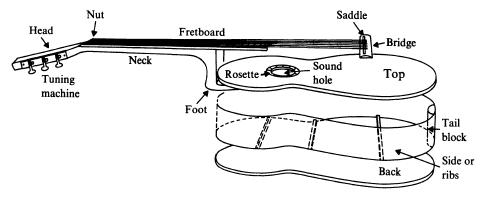
\includegraphics[width=0.85\linewidth]{00_Images/01_chapter/img59.jpg}
\caption{Exploded view of a classical guitar highlighting the main components}
\label{fig:guitar_exploded_view}
\end{figure}

Some construction features that are commonly specified are the following:

\begin{itemize}
    \item The instrument has six strings, about \SI{65}{\centi\meter} in length, tuned to \( E_2 \), \( A_2 \), \( D_3 \), \( G_3 \), \( B_3 \), and \( E_4 \), with fundamental frequencies
    \[
    f = \{\SI{82}{\hertz}, \SI{110}{\hertz}, \SI{147}{\hertz}, \SI{196}{\hertz}, \SI{247}{\hertz}, \SI{330}{\hertz}\}
    \]
    \item The top plate is usually cut from spruce or redwood, with thickness of about \SI{2.5}{\milli\meter}.
    \item The back plate is usually a hardwood, such as rosewood, mahogany, or maple, with thickness of about \SI{2.5}{\milli\meter}.
\end{itemize}

A key internal element of the soundboard is the bracing, namely a set of wooden strips glued to the inner side of the top plate. Bracing patterns alter the stiffness distribution of the soundboard and, as a consequence, strongly influence the vibrational behavior and the acoustic properties of the instrument. Several bracing layouts are commonly encountered or have been proposed over the years. Typical examples include traditional fan bracing, the Bouchet pattern (France), the Ramirez pattern (Spain), and crossed bracing, which uses intersecting braces to create an X-like reinforcement of the top plate. Representative bracing layouts are compared in figure \ref{fig:guitar_bracing_patterns}.

\begin{figure}[!htb]
\centering
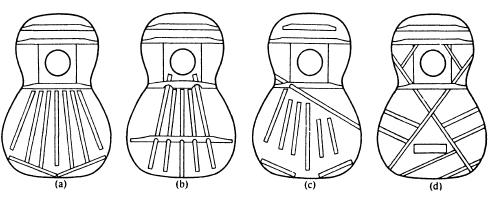
\includegraphics[width=0.95\linewidth]{00_Images/01_chapter/img77.jpg}
\caption{Examples of common soundboard bracing patterns for classical guitars}
\label{fig:guitar_bracing_patterns}
\end{figure}

\section{Excitation Mechanism in the Guitar: Plucking}

\subsection{Phases of the Plucking}

The excitation mechanism is crucial in plucked instruments because the first few milliseconds of the sound carry strong timbral cues: if this initial transient is removed, it becomes difficult to distinguish one instrument from another. Plucking can be described in terms of two main phases:

\begin{itemize}
    \item Stick phase: The string is displaced from its equilibrium position by an external force that can be idealized as concentrated at the plucking point \( x_0 \),
    \[
    F(x,t) = F_0\delta(x-x_0)
    \]
    As long as the applied force remains below a threshold \( F_{\mathrm{m}} \), the string stays stuck to the finger. In this phase a torsional component may also be present.
    \item Slip phase: When the restoring force reaches the threshold \( F_{\mathrm{m}} \), the string starts to slip under the finger. During slip, the finger or plectrum exerts a frictional force that introduces damping.
\end{itemize}

\subsection{Finger Articulation Model}

The finger can be modeled as a nonlinear spring with force-displacement relationship
\[
S(\xi)=
\begin{cases}
\dfrac{\sigma_1\xi}{\sigma_2-\xi} & \text{for } 0 \le \xi < \sigma_2 \\
\dfrac{\sigma_1\xi}{\sigma_2+\xi} & \text{for } -\sigma_2 < \xi < 0
\end{cases}
\]
This model captures an asymmetric, strongly nonlinear stiffness that increases rapidly as \( \xi \) approaches \( \pm\sigma_2 \), which is consistent with the limited range of finger articulation. The corresponding geometry and the nonlinear force-displacement characteristic are summarized in figure \ref{fig:finger_articulation_model}.

\begin{figure}[!htb]
\centering
\subfloat[]{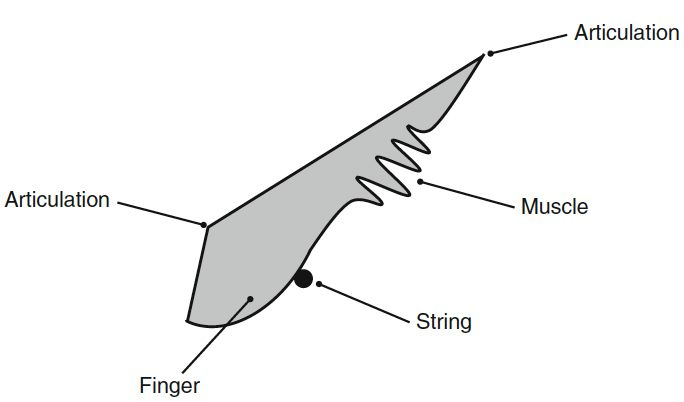
\includegraphics[width=0.45\linewidth]{00_Images/01_chapter/img127.jpg}}\hfill
\subfloat[]{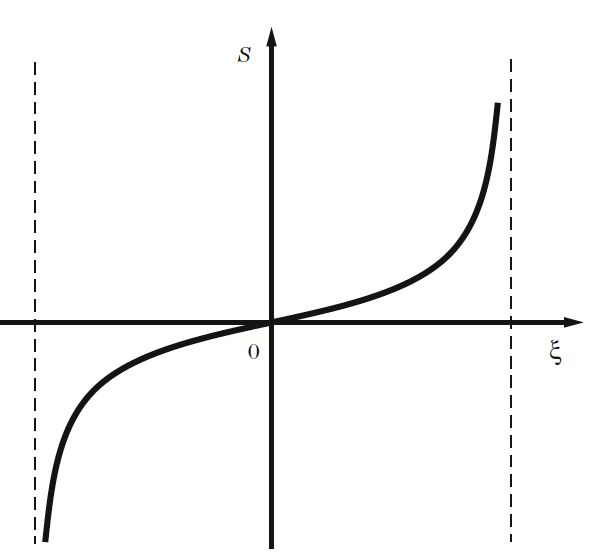
\includegraphics[width=0.45\linewidth]{00_Images/01_chapter/img129.jpg}}
\caption{Finger articulation model: schematic representation and nonlinear stiffness law}
\label{fig:finger_articulation_model}
\end{figure}

\subsection{Dynamic Friction Model of the Finger}

A dynamic description of the finger-string interaction considers different ingredients across the three stages of the motion.

\begin{itemize}
    \item During the stick phase: transversal motion of the string, rotation of the fingertip, torsional motion of the string, and the relative velocity between string and finger, which is ideally zero but may not be exactly so in practice.
    \item During the slip phase: the friction coefficient \( \mu \) depends on the relative velocity \( V_{\mathrm{rel}} \) between the string and the nail, according to
    \[
    \mu =
    \begin{cases}
    -\dfrac{\mu_S V_0 - \mu_d V_{\mathrm{rel}}}{V_{\mathrm{rel}} + V_0} & \text{for } V_{\mathrm{rel}} > 0  \\
    \dfrac{\mu_S V_0 - \mu_d V_{\mathrm{rel}}}{V_0 -    V_{\mathrm{rel}}} & \text{for } V_{\mathrm{rel}} < 0
    \end{cases}
    \]
    \item During free oscillations: the string motion is governed by transversal wave equations with two polarizations, perpendicular and parallel to the bridge, together with torsional dynamics.
\end{itemize}

A typical velocity-dependent friction law and a representative plucking-force time history are shown in figure \ref{fig:dynamic_friction_plucking_force}.

\begin{figure}[!htb]
\centering
\subfloat{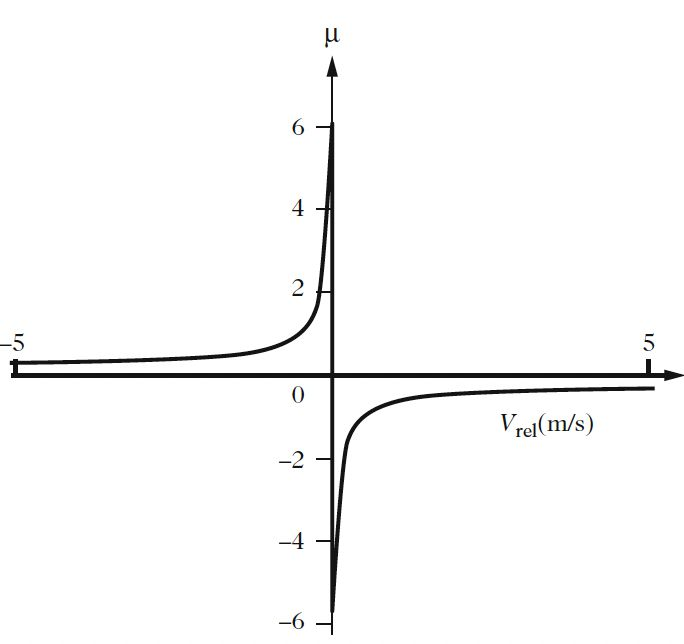
\includegraphics[width=0.45\linewidth]{00_Images/01_chapter/img151.jpg}}\hfill
\subfloat{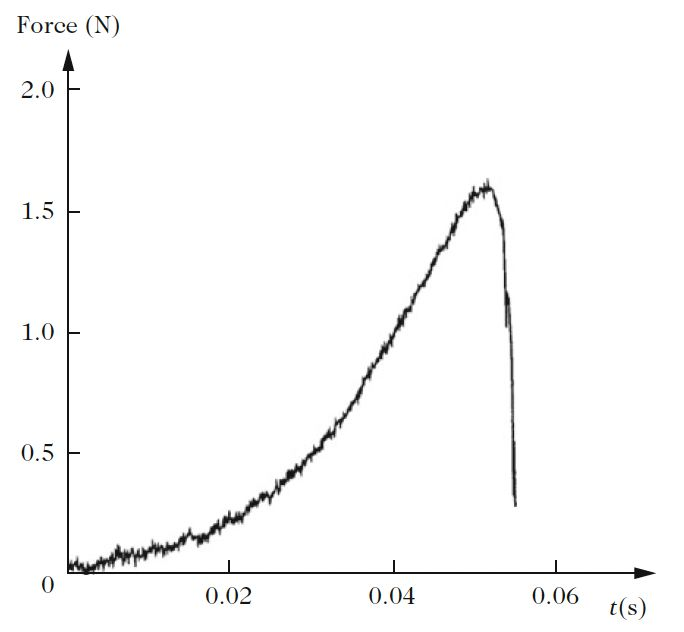
\includegraphics[width=0.45\linewidth]{00_Images/01_chapter/img153.jpg}}
\caption{Dynamic friction in plucking: friction coefficient versus relative velocity and an example force profile}
\label{fig:dynamic_friction_plucking_force}
\end{figure}

\section{The Guitar as a System of Coupled Vibrators}

\subsection{Sound Generation: Energy Flow in the Instrument}

Sound generation can be summarized as a chain of coupled subsystems. The strings mainly provide a driving force that sets the bridge region and the top plate into motion, and energy is then transferred to the enclosed air, the ribs, and the back. A simplified description of the main pathways is the following:

\begin{itemize}
    \item The strings put into vibration the bridge region and the top plate.
    \item Energy is transferred to the air cavity, ribs, and back plate.
    \item Sound is radiated efficiently by the top plate, the air cavity, and the back.
    \item At low frequency the top plate transmits energy to the back through both ribs and air cavity.
    \item At high frequency most of the sound is radiated by the top plate.
    \item At low frequency the bridge can be regarded as transparent, and it can be omitted from a minimal scheme.
\end{itemize}

A compact overview of the coupled subsystems involved in sound generation is shown in figure \ref{fig:guitar_energy_flow}.

\begin{figure}[!htb]
\centering
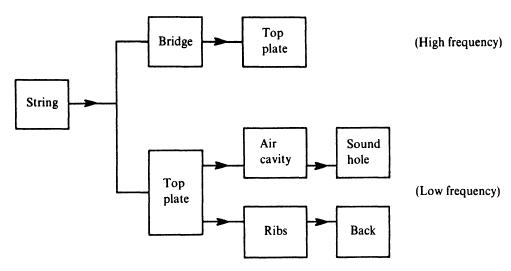
\includegraphics[width=0.9\linewidth]{00_Images/01_chapter/img170.jpg}
\caption{Energy flow and coupling pathways in the guitar body}
\label{fig:guitar_energy_flow}
\end{figure}

In what follows, a sequence of lumped-parameter models is introduced, with increasing complexity, in order to capture the low-frequency coupled behavior.

\subsection{Modeling by a Two-mass System}

If the motion of back and ribs is neglected, the guitar can be modeled as a two-degree-of-freedom vibrating system. The two subsystems are identified as follows:

\begin{itemize}
    \item The top plate, driven by the string force \( F(t) \), characterized by an effective mass \( m_p \) and stiffness \( K_p \).
    \item The Helmholtz resonator, represented by the mass of air \( m_h \) oscillating in the soundhole, while the enclosed air volume \( V \) provides the spring effect through compressibility.
\end{itemize}

An equivalent electrical circuit can be introduced, in which the analogous currents are volume velocities. The mechanical two-mass representation and the corresponding electrical analog are shown in figure \ref{fig:two_mass_electrical_analog}.

\begin{figure}[!htb]
\centering
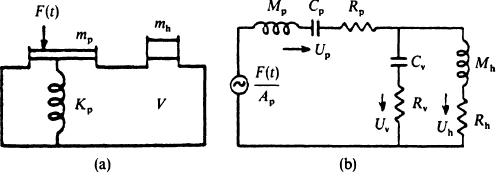
\includegraphics[width=0.95\linewidth]{00_Images/01_chapter/img189.jpg}
\caption{Two-mass guitar model and its electrical analog in terms of volume velocities}
\label{fig:two_mass_electrical_analog}
\end{figure}

\paragraph{Electrical analog and aymbols} In the electrical analog, the main quantities are expressed in terms of inertances and compliances. The symbols used are:

\begin{itemize}
    \item \( M_p = m_p/A_p^{2} \), inertance of the top plate.
    \item \( M_h = m_h/A_h^{2} \), inertance of the air in the soundhole.
    \item \( C_p = A_p^{2}/K_p \), compliance of the top plate.
    \item \( C_v = V/(\rho c^{2}) \), compliance of the enclosed air.
    \item \( U_p \), volume velocity of the top plate.
    \item \( U_h \), volume velocity of the air in the soundhole.
    \item \( U_v \), volume velocity associated with the air in the cavity.
    \item \( R_p \), losses (mechanical and radiative) associated with the top plate.
    \item \( R_h \), losses due to radiation from the soundhole.
    \item \( R_v \), losses associated with the enclosure.
\end{itemize}

\paragraph{Resonances and antiresonance} The coupled system exhibits two resonances with an antiresonance between them. Their qualitative interpretation can be summarized as follows:

\begin{itemize}
    \item At the lower resonance, the air flow through the soundhole is approximately in phase with the inward motion of the top plate, so that \( U_p \) and \( U_h \) are nearly in phase.
    \item At the upper resonance, air moves into the soundhole when the plate moves inward, leading to an out-of-phase relation between \( U_p \) and \( U_h \).
    \item The antiresonance corresponds to the Helmholtz resonance of the enclosure: \( U_v \) and \( U_h \) are equal and opposite, and consequently \( U_p \) reaches a minimum.
\end{itemize}

This circuit is able to capture the low-frequency response of a real guitar, for example when back plate and ribs are effectively immobilized. An example of measured low-frequency response consistent with the two-oscillator description is shown in figure \ref{fig:low_frequency_response_example}.

\begin{figure}[!htb]
\centering
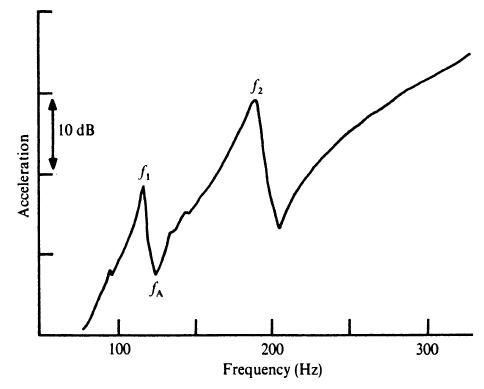
\includegraphics[width=0.7\linewidth]{00_Images/01_chapter/img204.jpg}
\caption{Example of low-frequency response captured by a minimal coupled model}
\label{fig:low_frequency_response_example}
\end{figure}

\subsection{Coupling at Low Frequencies between the Top Plate and the Cavity}

At low frequencies the interaction between the first (lowest) mode of the soundboard and the lowest acoustic mode of the cavity can be captured by a two-degree-of-freedom model. The soundboard is represented by a rigid body with mass \( m_p \), area \( A_p \), and intrinsic stiffness \( k_p \), subject to the vertical string force \( F \). Its vertical displacement is denoted by \( \xi_p \), interpreted as a mean displacement associated with the first structural mode. The soundbox is represented as a Helmholtz resonator with one moving wall. The inertial part is the mass of air \( m_h \) oscillating through holes of total area \( A_h \), with displacement \( \xi_h \). The volume change in the cavity is
\[
\Delta V = A_p \xi_p + A_h \xi_h
\]
Air compressibility produces a pressure change
\[
\Delta p = -\rho c^{2}\frac{\Delta V}{V} = -\mu\left(A_p \xi_p + A_h \xi_h\right)
\]
where
\[
\mu = \frac{\rho c^{2}}{V}
\]
Losses are modeled through a diagonal damping matrix with constants \( R_p \) for the plate and \( R_h \) for the soundbox, assumed approximately constant with frequency. The equations of motion can be written in matrix form as
\[
\begin{bmatrix}
m_p & 0 \\
0   & m_h
\end{bmatrix}
\begin{bmatrix}
\ddot{\xi}_p \\
\ddot{\xi}_h
\end{bmatrix}
+
\begin{bmatrix}
R_p & 0 \\
0   & R_h
\end{bmatrix}
\begin{bmatrix}
\dot{\xi}_p \\
\dot{\xi}_h
\end{bmatrix}
+
\begin{bmatrix}
k_p + \mu A_p^{2} & \mu A_h A_p \\
\mu A_h A_p       & \mu A_h^{2}
\end{bmatrix}
\begin{bmatrix}
\xi_p \\
\xi_h
\end{bmatrix}
=
\begin{bmatrix}
F \\
0
\end{bmatrix}
\]
Three limiting cases are useful to interpret the parameters:

\begin{itemize}
    \item With a closed hole, \( A_h = 0 \), the box acts on the board as an added stiffness \( \mu A_p^{2} \), and the undamped eigenfrequency becomes
    \[
    \omega_p = \sqrt{\frac{k_p + \mu A_p^{2}}{m_p}}
    \]
    \item If the board stiffness is negligible, the corresponding angular frequency becomes
    \[
    \omega_a = \sqrt{\frac{\mu A_p^{2}}{m_p}}
    \]
    \item If the board is held fixed, \( \xi_p = 0 \), the soundbox reduces to a Helmholtz resonator with
    \[
    \omega_h = \sqrt{\frac{\mu A_h^{2}}{m_h}}
    \]
\end{itemize}

The eigenfrequencies of the associated conservative coupled system satisfy
\[
\det\left(K - \omega^{2}M\right)=0
\]
which leads to
\[
\left(\omega_p^{2}-\omega^{2}\right)\left(\omega_h^{2}-\omega^{2}\right)-\omega_{ph}^{4}=0
\]
with
\[
\omega_{ph}^{4}=\omega_a^{2}\omega_h^{2}
\]
With typical guitar values, one finds for instance \( f_h \approx \SI{100}{\hertz} \) and \( f_a \approx \SI{200}{\hertz} \), leading to two split coupled resonances around \( f_1 \approx \SI{86}{\hertz} \) and \( f_2 \approx \SI{206.5}{\hertz} \). In this interpretation, \( f_1 \) is the Helmholtz resonance with non-rigid walls and \( f_2 \) is associated with the first top-plate mode \( T_1 \). The coupling therefore separates the original uncoupled frequencies, and it also holds that
\[
\omega_1^{2}+\omega_2^{2}=\omega_p^{2}+\omega_h^{2}
\]

\subsection{The Three-mass Model}

If the back plate is allowed to move, a three-oscillator model is obtained. In this case the ribs are assumed immobilized, and the coupling between top and back is enabled primarily by the air in the cavity. In the electrical analog, the back plate is represented by an inertance \( M_b \), a compliance \( C_b \), a loss \( R_b \), and a corresponding volume velocity \( U_b \). The response of this system is characterized by three resonances \( f_1 \), \( f_2 \), and \( f_3 \), and by two antiresonances \( f_A \) and \( f_B \). The three-oscillator electrical analog and its characteristic resonance/antiresonance pattern are shown in figure \ref{fig:three_mass_model}.

\begin{figure}[!htb]
\centering
\subfloat{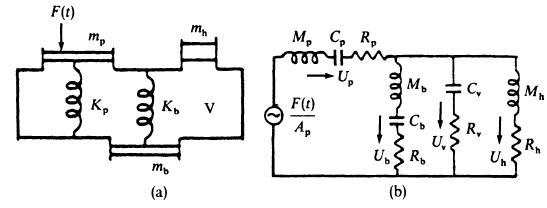
\includegraphics[width=0.58\linewidth]{00_Images/01_chapter/img300.jpg}}\hfill
\subfloat{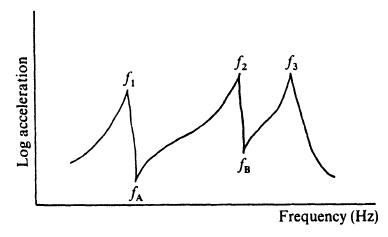
\includegraphics[width=0.38\linewidth]{00_Images/01_chapter/img319.jpg}}
\caption{Three-mass model: electrical analog and typical low-frequency response}
\label{fig:three_mass_model}
\end{figure}

\section{Structural Modifications of the Instrument}

Examples of construction differences and their impact on the vibrational/acoustical balance are illustrated in figure \ref{fig:structural_modifications_example}.

\begin{figure}[!htb]
\centering
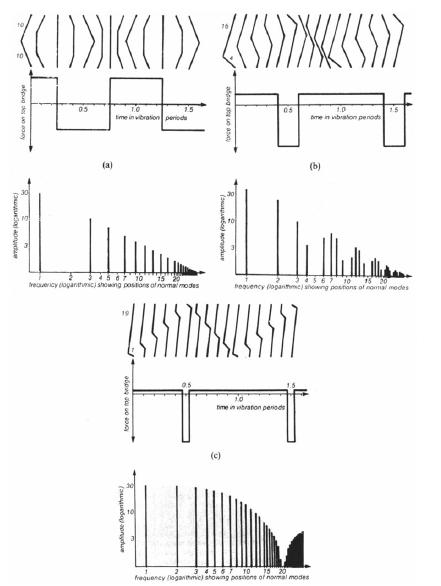
\includegraphics[width=0.7\linewidth]{00_Images/01_chapter/img481.jpg}
\caption{Illustrative example of structural modifications and associated spectral consequences}
\label{fig:structural_modifications_example}
\end{figure}

\subsection{Sensitivity of Eigenvalues to Structural Parameters}

To study how construction changes affect the low-frequency coupled behavior, it is convenient to consider the undamped generalized eigenvalue problem
\[
K \phi = \lambda M \phi
\]
where \( K \) is the stiffness matrix, \( M \) is the mass matrix, \( \phi \) is an eigenvector, and the eigenvalue is related to the angular eigenfrequency by
\[
\lambda = \omega^{2}
\]
Let \( a \) be a physical or geometrical parameter, such as a mass, a cavity volume, or the area of an opening. Differentiating the eigenvalue equation with respect to \( a \) gives
\[
\frac{\partial K}{\partial a}\phi + K\frac{\partial \phi}{\partial a}
=
\frac{\partial \lambda}{\partial a}M\phi + \lambda \frac{\partial M}{\partial a}\phi + \lambda M\frac{\partial \phi}{\partial a}
\]
From this relation, one obtains the sensitivity of the eigenvalues
\[
\frac{\partial \lambda}{\partial a}
=
\frac{\phi^{T}\dfrac{\partial K}{\partial a}\phi - \lambda \phi^{T}\dfrac{\partial M}{\partial a}\phi}{\phi^{T}M\phi}
\]
This expression links the frequency shifts directly to how the matrices \( K \) and \( M \) depend on the chosen parameter.

\subsection{Effect of Soundboard Mass}

Consider the two-degree-of-freedom model introduced earlier, with soundboard mass \( m_p \) and air mass in the soundhole \( m_h \). Setting \( a=m_p \), only the mass matrix is affected, and
\[
\frac{\partial M}{\partial m_p}
=
\begin{bmatrix}
1 & 0 \\
0 & 0
\end{bmatrix}
\]
If the mode shapes are assumed not to change significantly with a small modification of \( m_p \), the \( i \)-th eigenvalue sensitivity can be written as
\[
\frac{\partial \lambda_i}{\partial m_p}
=
-\frac{\lambda_i \phi_{i1}^{2}}{m_p\phi_{i1}^{2}+m_h\phi_{i2}^{2}}
\]
An increase of soundboard mass therefore reduces the eigenvalues and lowers the corresponding eigenfrequencies.

\subsection{Effect of Cavity Volume}

Setting \( a=V \), only the stiffness matrix changes through the cavity compliance. With \( \mu=\rho c^{2}/V \), one obtains
\[
\frac{\partial K}{\partial V}
=
-\frac{c^{2}\rho}{V^{2}}
\begin{bmatrix}
A_p^{2} & A_hA_p \\
A_hA_p  & A_h^{2}
\end{bmatrix}
\]
and the sensitivity becomes
\[
\frac{\partial \lambda_i}{\partial V}
=
-\frac{\dfrac{c^{2}\rho}{V^{2}}\left(A_p^{2}\phi_{i1}^{2}+2A_pA_h\phi_{i1}\phi_{i2}+A_h^{2}\phi_{i2}^{2}\right)}{m_p\phi_{i1}^{2}+m_h\phi_{i2}^{2}}
\]
An increase of the soundbox volume lowers the eigenfrequencies, which is consistent with the historical trend toward larger-bodied instruments.

\subsection{Effect of Soundhole Area and Thickness}

The mass of air in the opening can be written as
\[
m_h = \rho h A_h
\]
where \( h \) is an effective thickness of the opening. A change in opening area \( A_h \) affects both stiffness and mass:
\[
\frac{\partial K}{\partial A_h}
=
\mu
\begin{bmatrix}
0   & A_p \\
A_p & 2A_h
\end{bmatrix}
\quad
\frac{\partial M}{\partial A_h}
=
\begin{bmatrix}
0 & 0 \\
0 & \rho h
\end{bmatrix}
\]
leading to
\[
\frac{\partial \lambda_i}{\partial A_h}
=
\frac{2\mu\left(A_p\phi_{i1}\phi_{i2}+A_h\phi_{i2}^{2}\right)-\lambda_i\rho h\phi_{i2}^{2}}{m_p\phi_{i1}^{2}+m_h\phi_{i2}^{2}}
\]
In this simplified setting, increasing the total area of the openings tends to increase the eigenfrequencies, while increasing the effective thickness \( h \) has the opposite effect through the added air mass.

\subsection{Effect of Soundboard Thickness and Bracing}

Makers commonly modify the overall stiffness of the soundboard either by varying its thickness or by adding stiffeners (bracing), or both. If the thickness \( e \) is varied, the mass scales approximately in proportion to \( e \), whereas the bending stiffness scales approximately as \( e^{3} \), so stiffness changes can dominate. For simplicity, one may isolate the effect of an effective plate stiffness \( k_p \), keeping \( m_p \) fixed. With \( a=k_p \), the sensitivity becomes
\[
\frac{\partial \lambda_i}{\partial k_p}
=
\frac{\phi_{i1}^{2}}{m_p\phi_{i1}^{2}+m_h\phi_{i2}^{2}}
\]
An increase of \( k_p \) raises the eigenfrequencies, while a decrease of thickness, which typically reduces effective stiffness, lowers them.

\section{Modeling of Plucked Strings}

\subsection{Force Exerted by the Strings}

When a string is plucked, the tension \( T \) applies a force to the bridge that can be decomposed into a component normal to the top plate and a component parallel to it. Let \( \theta \) be the plucking angle. The two components are
\[
T\sin\theta \quad \text{(normal to the plate)}, \qquad T\cos\theta \quad \text{(parallel to the plate)}
\]
During the vibration cycle the string length changes slightly, which induces a time-varying tension. If \( A \) is the string cross-section, \( E \) its Young's modulus, and \( L_0 \) the nominal length, the tension can be written as
\[
T = T_0 + \Delta T = T_0 + \frac{EA}{L_0}\Delta L
\]
For small \( \theta \), the transverse and longitudinal force components at the bridge become
\[
F_T = (T_0+\Delta T)\sin\theta
\]
\[
F_L = (T_0+\Delta T)\cos\theta \simeq T_0+\Delta T = T_0 + \frac{EA}{L_0}\Delta L
\]
Consider a string displaced by a distance \( d \) at a point located at \( \beta L_0 \) from the bridge and then released. The two string segments form angles \( \theta_1 \) and \( \theta_2 \) with
\[
\sin\theta_1 \simeq \frac{d}{\beta L_0}
\qquad
\sin\theta_2 = \frac{d}{(1-\beta)L_0}
\]
The longitudinal force component \( F_L \) has a slight time dependence due to the change in string length during the cycle. The maximum elongation can be estimated from the two-segment geometry as
\[
\Delta L_{\max}
=
\sqrt{\beta^{2}L_{0}^{2}+d^{2}}
+
\sqrt{(1-\beta)^{2}L_{0}^{2}+d^{2}}
-
L_{0}
\]
A minimum elongation is reached when the bend is located at \( 2\beta L_0 \), leading to
\[
\Delta L_{\min}
=
\sqrt{4\beta^{2}L_{0}^{2}+\frac{(1-2\beta)^{2}}{(1-\beta)^{2}}d^{2}}
+
\sqrt{(1-2\beta)^{2}L_{0}^{2}+\frac{(1-2\beta)^{2}}{(1-\beta)^{2}}d^{2}}
-
L_{0}
\]
Some qualitative consequences follow from the previous relations:

\begin{itemize}
    \item For nylon strings and small \( d \), the transverse component can largely dominate the longitudinal one, \( F_T \gg F_L \).
    \item The coupling between transverse string motion and top-plate motion is typically more effective than the coupling associated with the parallel component.
    \item Increasing \( d \) increases the relevance of the component parallel to the plate.
    \item For steel strings the difference between \( F_L \) and \( F_T \) is generally less pronounced.
\end{itemize}

The plucking position also matters. As \( \beta \) decreases, both transverse and longitudinal forces increase, while at the same time a larger applied effort is required to reach the same deflection \( d \). This is reflected in the waveform and in the corresponding spectrum, which change noticeably when the pluck is moved closer to the bridge. Typical changes in waveform and spectrum as the plucking point approaches the bridge are shown in figure \ref{fig:pluck_position_waveform_spectrum}.

\begin{figure}[!htb]
\centering
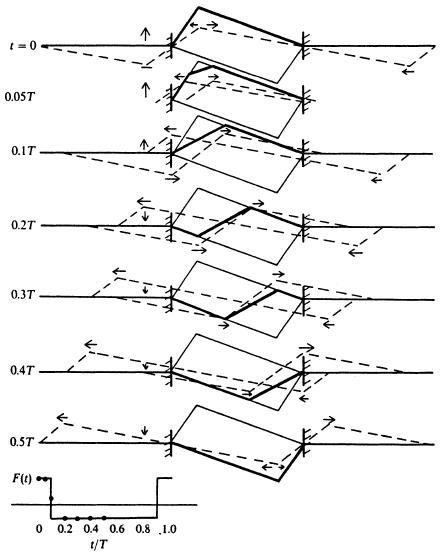
\includegraphics[width=0.7\linewidth]{00_Images/01_chapter/img495.jpg}
\caption{Influence of plucking position on time waveform and corresponding spectrum}
\label{fig:pluck_position_waveform_spectrum}
\end{figure}

\subsection{Modeling}

In the coupled models introduced earlier, attention was focused on transfer functions, without explicitly describing the excitation. For a plucked string, the initial condition produced by the pluck strongly shapes the waveform and therefore the radiated sound. A standard description of string motion is based on the superposition of two traveling waves propagating in opposite directions and reflecting at the terminations. Under the assumption that, during autonomous vibration, the string can be regarded as a linear time-invariant system, this leads to efficient computational models. A widely used representation is the bidirectional digital waveguide: two delay lines implement the propagation in the two directions, while reflection filters \( R_f(z) \) and \( R_b(z) \) account for phase inversion and frequency-dependent losses at the terminations. In this view, input and output signals may represent different wave variables, such as displacement, velocity, acceleration, or slope. Choosing acceleration as the wave variable is convenient, because an idealized pluck can be treated as an impulse-like excitation. For sound synthesis, it is often advantageous to commute propagation, losses, and dispersion into a single delay-loop structure. In this simplified single delay-loop model, the effects of losses and dispersion are lumped into a loop filter \( H_l(z) \). A particularly simple special case uses a two-point averaging loop filter and random initial conditions in the delay line, yielding the Karplus-Strong algorithm. This extreme simplification is computationally efficient but generally insufficient for high-quality synthesis or detailed physical interpretation. To connect the bidirectional waveguide description to an efficient single-loop form while preserving excitation and observation positions, it is useful to derive an equivalent linear transfer function for a given output, such as the transverse force at the bridge. In the Laplace domain, an equivalent single excitation at point \( E_1 \) can be introduced as
\[
X_{E_1,\mathrm{eq}}(s)
=
\frac{1}{2}\left[1+H_{E_2,E_1}(s)\right]X(s)
=
H_E(s)X(s)
\]
The bridge output of interest is the transverse force \( F(s) \), which can be related to the bridge impedance \( Z(s) \) and to the difference of the counter-propagating velocity components. Using accelerations \( A_1(s) \) and \( A_2(s) \),
\[
F(s)=Z(s)\frac{A_1(s)-A_2(s)}{s}
\]
If the backward-traveling component is expressed through a reflection \( R_b(s) \), this becomes
\[
F(s)=Z(s)\frac{\left[1-R_b(s)\right]A_1(s)}{s}=H_B(s)A_1(s)
\]
The acceleration at the bridge satisfies a recursion of the form
\[
A_1(s)=H_{E_1,R_1}(s)X_{E_1,\mathrm{eq}}(s)+H_{\mathrm{loop}}(s)A_1(s)
\]
with a loop transfer function
\[
H_{\mathrm{loop}}(s)=R_b(s)H_{R_2,E_2}(s)H_{E_2,E_1}(s)H_{E_1,R_1}(s)
\]
Solving for \( A_1(s) \) yields
\[
A_1(s)=H_{E_1,R_1}(s)\frac{1}{1-H_{\mathrm{loop}}(s)}X_{E_1,\mathrm{eq}}(s)
=
H_{E_1,R_1}(s)S(s)X_{E_1,\mathrm{eq}}(s)
\]
where \( S(s) \) represents the recursion around the loop. The overall transfer function from excitation to bridge force is then obtained by cascading the equivalent excitation, propagation, loop recursion, bridge coupling, and integration. A perceptually equivalent block diagram can be constructed by grouping the effects of excitation position, bridge coupling, and the integrator into a small set of filters around a delay-loop. In this interpretation, excitation position produces a comb-filter-like effect on the harmonic amplitudes, which is stronger as the pluck is moved away from the midpoint.

\subsection{Modeling of High-frequency Resonances}

The lumped analogs introduced for the body capture the low-frequency coupled behavior well, but they become insufficient at higher frequencies. To extend the validity, the body response can be analyzed in the frequency domain and each significant resonance can be rendered by a separate damped oscillator. Low-frequency oscillators retain a clear physical interpretation from the coupled models, while higher-frequency resonances are introduced by fitting the measured or computed frequency response.

\subsection{Coupling of Different Components}

A complete model can be assembled by coupling the string model to an electrical analog of the guitar body. In this representation, a resonant branch associated with the top plate is combined with elements representing the soundbox resonance and additional losses. The resulting network can reproduce both magnitude and phase of the body frequency response over a wider band when parameters are chosen consistently with measurements. A representative electrical analog for the guitar body used in coupled simulations is shown in figure \ref{fig:complete_body_model} and an example of agreement in both magnitude and phase for the body frequency response is shown in figure \ref{fig:body_frf_mag_phase}. The integration of the string model with the body analog is summarized in figure \ref{fig:string_body_integration}.

\subsection{Waveforms and Spectrograms}

Once string and body models are integrated, time-domain signals such as bridge velocity and force can be synthesized and compared with recorded quantities. Waveforms and corresponding spectrograms provide a compact way to verify whether the temporal evolution and the spectral envelope produced by the model are consistent with the measured excitation force and the recorded sound. A representative set of waveforms and the corresponding spectrograms is shown in figure \ref{fig:waveforms_spectrograms}.

\begin{figure}[!htb]
\centering
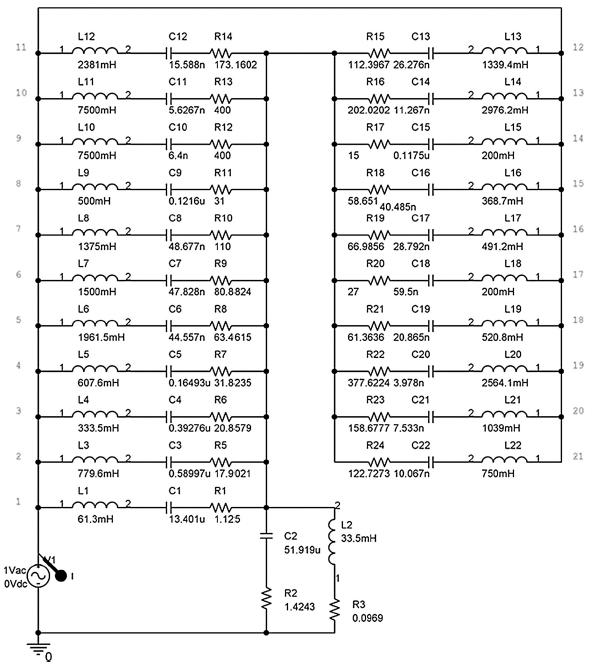
\includegraphics[width=0.8\linewidth]{00_Images/01_chapter/img554.jpg}
\caption{Electrical analog of the guitar body for broadband modeling}
\label{fig:complete_body_model}
\end{figure}

\begin{figure}[!htb]
\centering
\subfloat{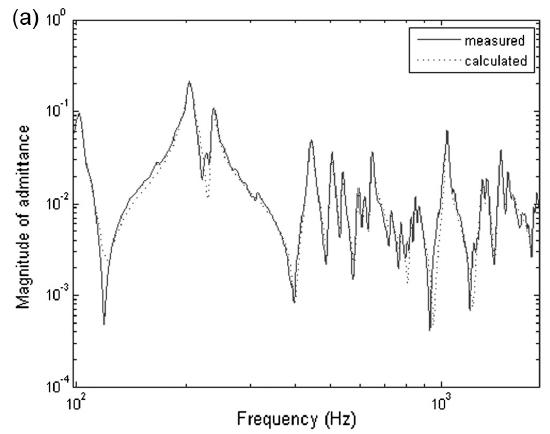
\includegraphics[width=0.45\linewidth]{00_Images/01_chapter/img568.jpg}}\hfill
\subfloat{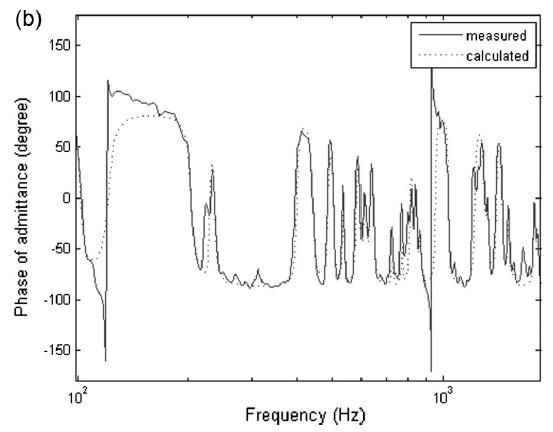
\includegraphics[width=0.45\linewidth]{00_Images/01_chapter/img578.jpg}}
\caption{Body frequency response function: magnitude and phase comparison}
\label{fig:body_frf_mag_phase}
\end{figure}

\begin{figure}[!htb]
\centering
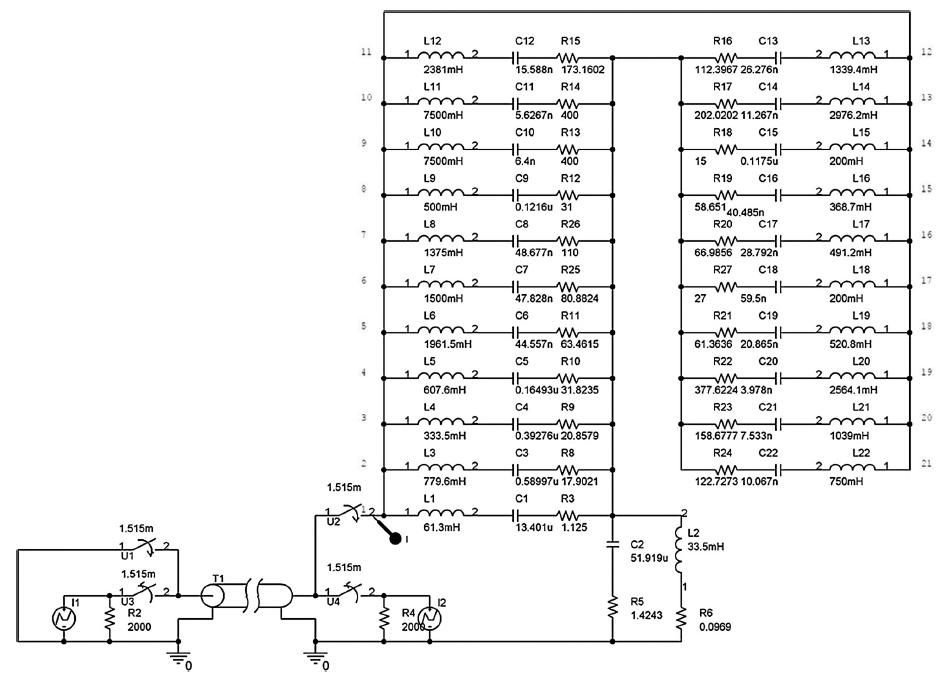
\includegraphics[width=0.7\linewidth]{00_Images/01_chapter/img592.jpg}
\caption{Integration of string and body models within a unified network representation}
\label{fig:string_body_integration}
\end{figure}

\begin{figure}[!htb]
\centering
\subfloat{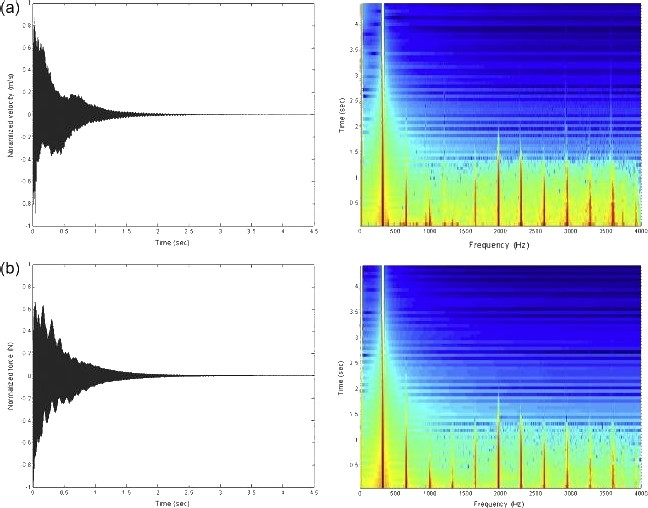
\includegraphics[width=0.45\linewidth]{00_Images/01_chapter/img606_1.jpg}}\hfill
\subfloat{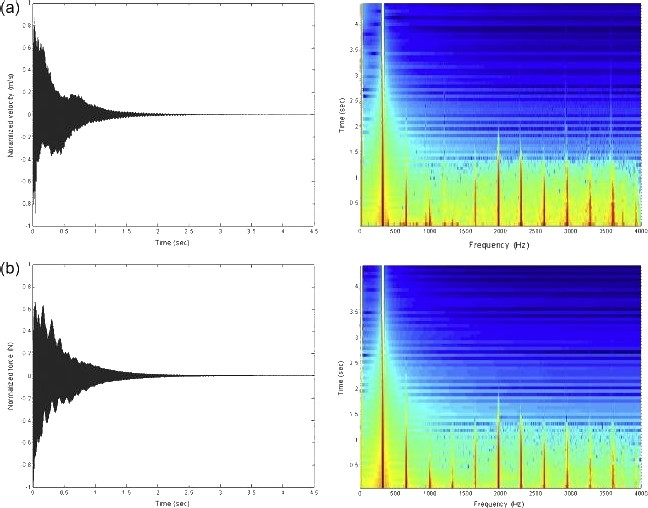
\includegraphics[width=0.45\linewidth]{00_Images/01_chapter/img606_1.jpg}}
\caption{Simulated or measured waveforms and corresponding spectrograms for model validation}
\label{fig:waveforms_spectrograms}
\end{figure}

\section{Response to String Forces}

The string action at the bridge can be decomposed into components that are parallel and orthogonal with respect to the bridge line. These components couple differently to the low-order vibration shapes of the soundboard. The main qualitative effects can be summarized as follows:

\begin{itemize}
    \item The force component parallel to the bridge is typically smaller in magnitude, but it promotes a rocking motion of the bridge, especially when the excitation is applied on one side of the bridge.
    \item The soundboard mode that is most efficiently excited by the horizontal, bridge-parallel action is the \( (1,0) \) mode.
    \item A force component orthogonal to the bridge can strongly excite the fundamental \( (0,0) \) resonance.
    \item If the orthogonal component is applied preferentially toward the treble or bass side, it can also excite the \( (1,0) \) mode.
\end{itemize}

\paragraph{Evidence from holographic interferometry} The different coupling mechanisms can be visualized through holographic interferograms of the top plate under controlled static actions. Distinct deformation patterns are observed when applying a lateral force parallel to the bridge, a force perpendicular to the bridge, a longitudinal force, or a twisting torque, confirming that the direction and point of application of the string-induced loading select different families of soundboard motion. Representative holographic interferograms illustrating the dependence on loading direction are shown in figure \ref{fig:holographic_interferograms}.

\begin{figure}[!htb]
\centering
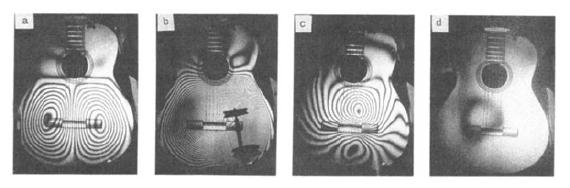
\includegraphics[width=0.8\linewidth]{00_Images/01_chapter/img622.jpg}
\caption{Holographic interferograms of the soundboard under different static actions at the bridge}
\label{fig:holographic_interferograms}
\end{figure}

\paragraph{Compound decay in normal plucking} In normal playing, the pluck direction is neither purely parallel nor purely orthogonal to the bridge, so both components are present at once. The orthogonal component tends to excite modes that are strong but decay rapidly, while the parallel component activates modes that are weaker but decay more slowly. As a result, the observed vibration envelope often shows a compound decay, with a fast initial reduction followed by a longer-lasting tail. An example of compound decay resulting from the coexistence of fast and slow modal components is shown in figure \ref{fig:compound_decay}.

\begin{figure}[!htb]
\centering
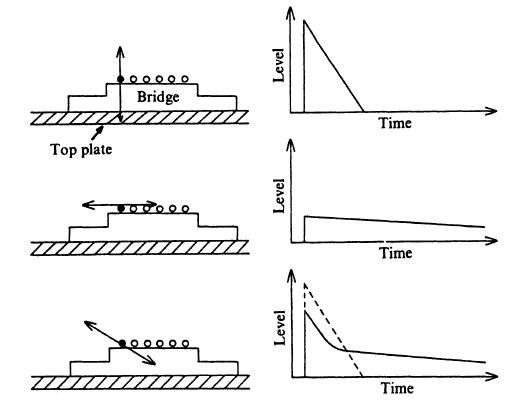
\includegraphics[width=0.6\linewidth]{00_Images/01_chapter/img636.jpg}
\caption{Example of compound decay envelope in normal plucking}
\label{fig:compound_decay}
\end{figure}

\section{Sound Radiation}

Sound radiation from the guitar is the result of a complex superposition of the radiation contributions associated with many structural and acoustic modes. Some low-frequency modes can radiate efficiently even when the instrument is driven well above their natural frequency, producing a smoothing effect on the resulting spectrum.

\paragraph{Mechanical response and radiated spectrum} A representative comparison can be made by considering a Martin D-28 guitar driven by a sinusoidal force of \SI{0.15}{\newton} applied at the treble side of the bridge, and observing the sound spectrum at \SI{1}{\meter} in front of the instrument. The measured acceleration level at the driving point highlights the mechanical resonances, while the radiated sound spectrum follows the overall trend but does not replicate it one-to-one, because radiation efficiency varies with frequency and mode shape. A representative comparison between mechanical response at the driving point and the radiated sound spectrum is shown in figure \ref{fig:mech_vs_radiated_spectrum}.

\begin{figure}[!htb]
\centering
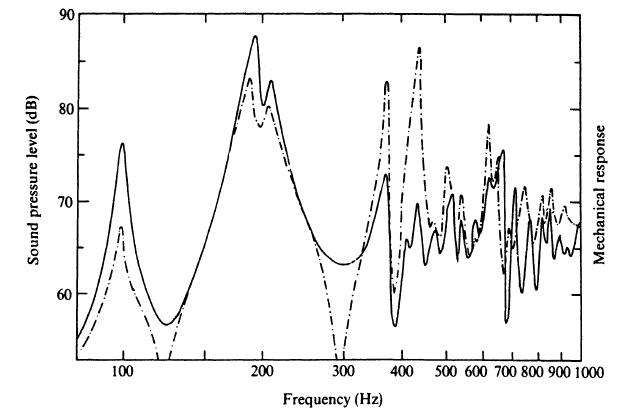
\includegraphics[width=0.45\linewidth]{00_Images/01_chapter/img654.jpg}
\caption{Driving-point mechanical response and radiated sound spectrum under sinusoidal forcing}
\label{fig:mech_vs_radiated_spectrum}
\end{figure}

\paragraph{Radiation patterns at resonances} Radiation directivity changes significantly across resonances. At lower frequencies, the patterns tend to be comparatively smooth, whereas at higher resonances the angular distribution becomes more structured, with multiple lobes and nulls. For instance, radiation patterns reported around \SI{102}{\hertz}, \SI{204}{\hertz}, \SI{376}{\hertz}, and \SI{436}{\hertz} show an evolution from simpler to more complex directivity shapes as frequency increases. Examples of measured radiation directivity at selected resonances are shown in figure \ref{fig:radiation_patterns_resonances}.

\begin{figure}[!htb]
\centering
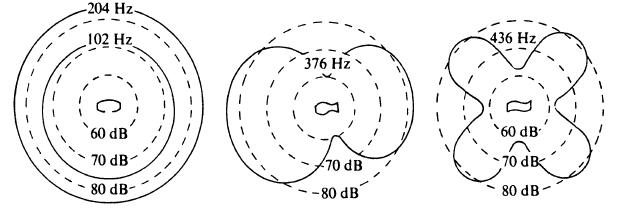
\includegraphics[width=0.7\linewidth]{00_Images/01_chapter/img668.jpg}
\caption{Radiation patterns at selected resonances illustrating the evolution of directivity with frequency}
\label{fig:radiation_patterns_resonances}
\end{figure}

    %! TEX rootmain.tex

\chapter{Piano}

The piano combines a percussive excitation mechanism with a large resonant structure. A key press triggers a sequence of mechanical events that culminates in string vibration, energy transfer through the bridge, and sound radiation by the soundboard. Following the course outline, the discussion starts from the instrument anatomy and then moves to the piano action, strings and hammers, the role of the soundboard, sound decay, and finally tuning and inharmonicity.

\section{Anatomy of the Instrument}

A simplified scheme of the piano highlights four main subsystems: the keyboard and action, the strings, the soundboard, and the structural frame. Their interaction determines both the mechanical response and the acoustic output. A simplified block diagram of the piano highlights the main coupled subsystems, as shown in figure \ref{fig:piano_simplified_scheme}.

\begin{figure}[!htb]
\centering
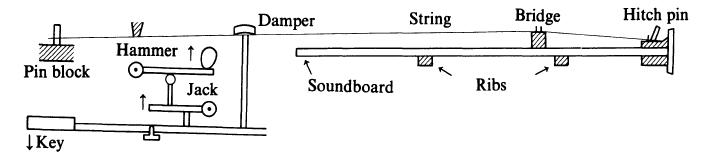
\includegraphics[width=0.9\linewidth]{00_Images/02_chapter/img37.jpg}
\caption{Simplified scheme of the piano as coupled subsystems from key to soundboard}
\label{fig:piano_simplified_scheme}
\end{figure}

\subsection{From Key Press to Soundboard Vibration}

When a key is depressed, the sound production chain can be described as a sequence of coupled events. In compact form, the process is the following:

\begin{itemize}
    \item The damper is raised, allowing the string to vibrate.
    \item The action throws the hammer against the strings.
    \item The strings are set into vibration.
    \item The string vibration is transmitted to the soundboard through the bridge.
\end{itemize}

Each step has been progressively refined in historical development, because small improvements in the action and in the structural design strongly affect controllability, repeatability, and tonal result.

\subsection{Strings Layout in a Grand Concert}

A grand concert piano contains a large number of strings, with geometrical and material variations across the compass. Typical figures are as follows:

\begin{itemize}
    \item The total number of strings is about 243, with lengths ranging from about \SI{2}{\meter} in the bass to about \SI{5}{\centi\meter} in the treble.
    \item 68 notes are produced by triplets of unwrapped strings.
    \item 7 notes are produced by three wrapped strings.
    \item 5 notes are produced by pairs of wrapped strings.
    \item 8 notes are produced by single strings wrapped with one or two layers of wire.
\end{itemize}

A relevant construction detail is that bass strings overlap middle strings in order to locate their action closer to the center of the soundboard. A representative layout of strings and soundboard in a grand concert is shown in figure \ref{fig:grand_strings_layout}.

\begin{figure}[!htb]
\centering
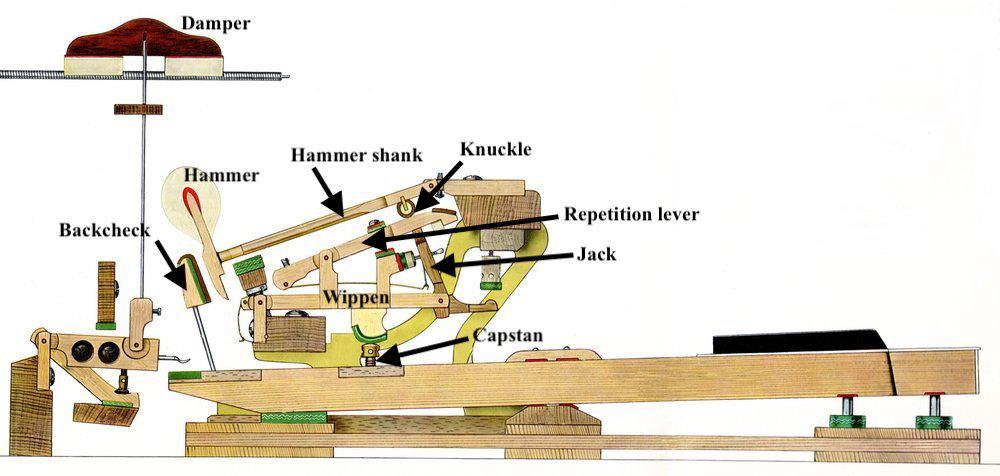
\includegraphics[width=0.8\linewidth]{00_Images/02_chapter/img43.jpg}
\caption{Typical strings layout and soundboard arrangement in a grand concert piano}
\label{fig:grand_strings_layout}
\end{figure}

\subsection{Soundboard and Frame}

The soundboard is typically made from spruce, with thickness up to about \SI{1}{\centi\meter} and grain running along the length of the piano. Ribs beneath the board stiffen it in the cross-grain direction. Besides its radiating role, the soundboard assembly has an important static function, because the total string tension can be very large. In a grand piano the overall force may exceed \SI{20}{\tonne}, and robust cast-iron frames are required to withstand the load while maintaining tuning stability.

\subsection{Upright Piano Variants and Striking Mechanism}

Upright pianos may vary considerably in design, mainly because the striking mechanism differs from the grand. The hammer motion is horizontal, so the return of parts to their rest position depends on springs. Three representative arrangements are commonly distinguished:

\begin{itemize}
    \item In a full-size upright, the striking mechanism is located above the keys and connected to them through sticks.
    \item In a studio upright, the action is mounted directly over the keys, without sticks.
    \item In a small spinet, the action is below the keys, and drop sticks transmit the key motion to the action.
\end{itemize}

Common upright variants and their main geometric differences are compared in figure \ref{fig:upright_variants}.

\begin{figure}[!htb]
\centering
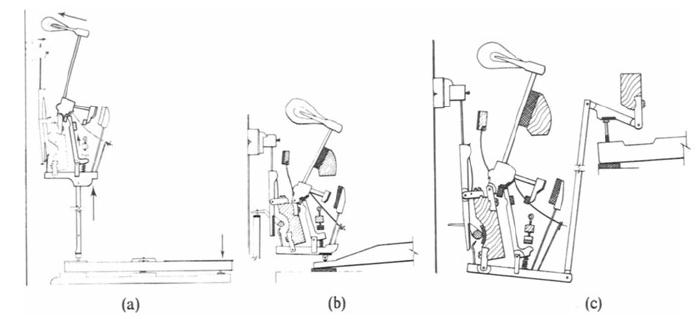
\includegraphics[width=0.8\linewidth]{00_Images/02_chapter/img58.jpg}
\caption{Examples of upright piano variants and corresponding construction differences}
\label{fig:upright_variants}
\end{figure}

\section{Piano Action}

\subsection{Kinematic Sequence During a Keystroke}

When a key is pressed down, the piano action converts the finger force into a fast hammer motion through a sequence of constrained movements and releases. The main stages can be summarized as follows:

\begin{itemize}
    \item The wippen, jack, and hammer are raised.
    \item The key begins to raise the damper, freeing the string.
    \item The jack engages the regulator and rotates away from the knuckle.
    \item After impact, the hammer rebounds and is caught by the backcheck, while the knuckle depresses the repetition lever.
    \item If the key is released slightly, the backcheck releases the hammer and the repetition lever lifts it until the jack returns below the knuckle, enabling repetition.
\end{itemize}

The main phases of the action motion during a keystroke are summarized in figure \ref{fig:piano_action_sequence}.

\begin{figure}[!htb]
\centering
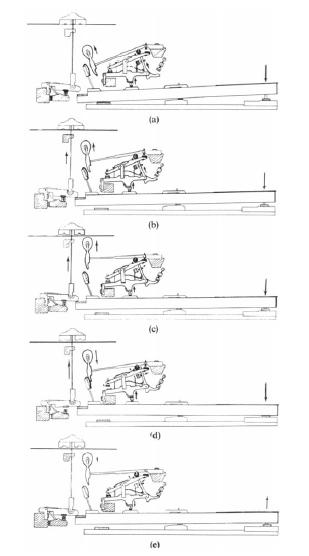
\includegraphics[width=0.7\linewidth]{00_Images/02_chapter/img85.jpg}
\caption{Kinematic sequence of the piano action during a keystroke}
\label{fig:piano_action_sequence}
\end{figure}

\subsection{Simplified Lever Model}

To connect the player input to the mechanical outcome, a simplified diagram models the action as two levers transmitting a key depression force \( F \) applied at the touch point \( P \). During the acceleration phase, the touch point moves with velocity \( v_p(t) \), while the hammer velocity is \( v_h(t) \). A typical effective velocity ratio is approximately constant for most of the touch, and then the hammer swings free. A simplified lever representation of the action is shown in figure \ref{fig:simplified_lever_model}.

\begin{figure}[!htb]
\centering
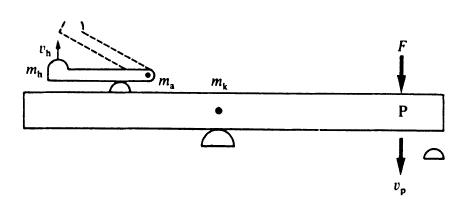
\includegraphics[width=0.6\linewidth]{00_Images/02_chapter/img117.jpg}
\caption{Simplified lever model relating key motion, contact point, and hammer motion}
\label{fig:simplified_lever_model}
\end{figure}

\subsection{Equation of Motion and Touch Acceleration}

During about \SI{70}{\percent} of the touch, the velocity ratio is approximately
\[
\frac{v_h}{v_p} = 5.5
\]
The static force needed to raise the key is about
\[
F_s = \SI{0.44}{\newton}
\]
which is equivalent to raising a mass of about \SI{45}{\gram}. In addition to \( F_s \), the applied force must accelerate the moving parts of the key and action. With \( m_k \) the effective key mass, \( m_a \) the equivalent mass of other action parts, \( m_h \) the hammer mass, and \( a_p \) the acceleration at the touch point, the equation of motion is written as
\[
F - F_s = m_k(0.018a_p) + m_a(0.72a_p) + m_h(5.5a_p)
\]
By substituting typical numerical values, the touch acceleration becomes
\[
a_p = \frac{dv_p}{dt} = 3.3(F-\SI{0.44}{\newton})
\]

\subsection{Key Travel Time and Hammer Striking Velocity}

If the depressing force is assumed constant over the key travel, the time \( T_s \) needed to move through a distance \( s \) to the stop is
\[
T_s = \sqrt{\frac{2s}{a_p}}
\]
For a typical travel \( s=\SI{9}{\milli\meter} \), this yields
\[
T_s = 0.074\sqrt{(F-\SI{0.44}{\newton})}
\]
The hammer striking velocity \( V_0 \) follows from the velocity ratio during the constrained phase,
\[
V_0 = 5.5a_pT_s = 1.34\sqrt{(F-\SI{0.44}{\newton})}
\]
A plot of \( V_0 \) and \( T_s \) as a function of \( F \) shows that increasing force produces a larger striking velocity and a shorter key depression time, with indicative regions corresponding to dynamic levels from \( pp \) to \( ff \). The dependence of striking velocity and travel time on applied force is illustrated in figure \ref{fig:striking_velocity_travel_time}.

\begin{figure}[!htb]
\centering
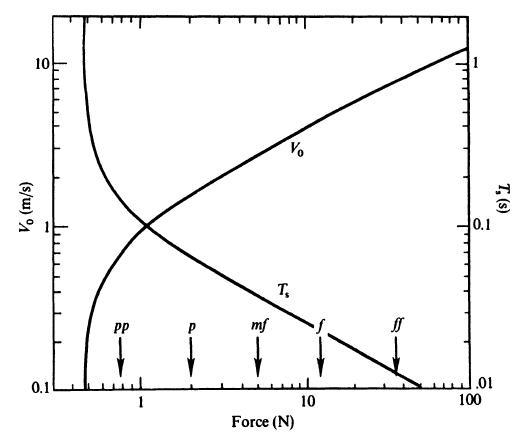
\includegraphics[width=0.6\linewidth]{00_Images/02_chapter/img132.jpg}
\caption{Hammer striking velocity and key travel time versus applied force}
\label{fig:striking_velocity_travel_time}
\end{figure}

\subsection{Non-constant Force Profiles and Timing Control}

If the applied force is not constant in time, the same striking velocity, and therefore a comparable impact strength on the strings, can be obtained with different key depressing times. Skilled players can exploit this by controlling timing within a chord, making one note sound slightly earlier or later than the others while maintaining similar intensity.

\subsection{Pedals and Their Functions}

Pianos typically have two or three pedals, modifying sustain and excitation conditions.

\begin{itemize}
    \item The right pedal is the sustaining pedal and lifts the dampers, so struck strings continue vibrating after the keys are released.
    \item The left pedal differs between grand and upright designs. In most grands it shifts the action sideways so that treble hammers strike two strings instead of three, called the una corda pedal. In many uprights, and in some grands, it moves the hammers closer to the strings, reducing travel and striking force, often called the soft pedal.
    \item The third pedal may act as a sostenuto pedal, sustaining only notes already depressed when the pedal is engaged. In some instruments it lifts only bass dampers, while in some uprights it functions as a practice pedal by inserting felt between hammers and strings to mute the tone.
\end{itemize}

\section{Piano Strings}

Strings have the fundamental task of capturing the energy brought by the hammer, converting it into vibrational energy, storing it in their normal modes, and transmitting this energy to the bridge and soundboard.

\subsection{Materials, Tension, and Construction} 

Piano strings are high-strength steel wires. In order to produce tones with the expected loudness, high tensions are used: the tensile stress is around
\[
\sigma \approx \SI{1000}{\newton\per\milli\meter\squared}
\]
For steel, this corresponds to an elongation of about
\[
\varepsilon \approx \SI{0.5}{\percent}
\]
Treble strings are solid wire, while lower strings are wound with copper wire. The winding diameter varies widely across the compass, from about twice the core diameter for the lowest string to about one fourth for the highest wrapped string. The winding is mainly used to increase mass per unit length while minimizing bending stiffness. Strings are clamped on one side and pinned on the other, so the normal modes are expected to lie between those of clamped-clamped and pinned-pinned stiff strings. In practice, expressions for pinned stiff strings are commonly used as a workable approximation. Typical trends of tension and inharmonicity along the keyboard are summarized in figure \ref{fig:string_scales_trends}.

\begin{figure}[!htb]
\centering
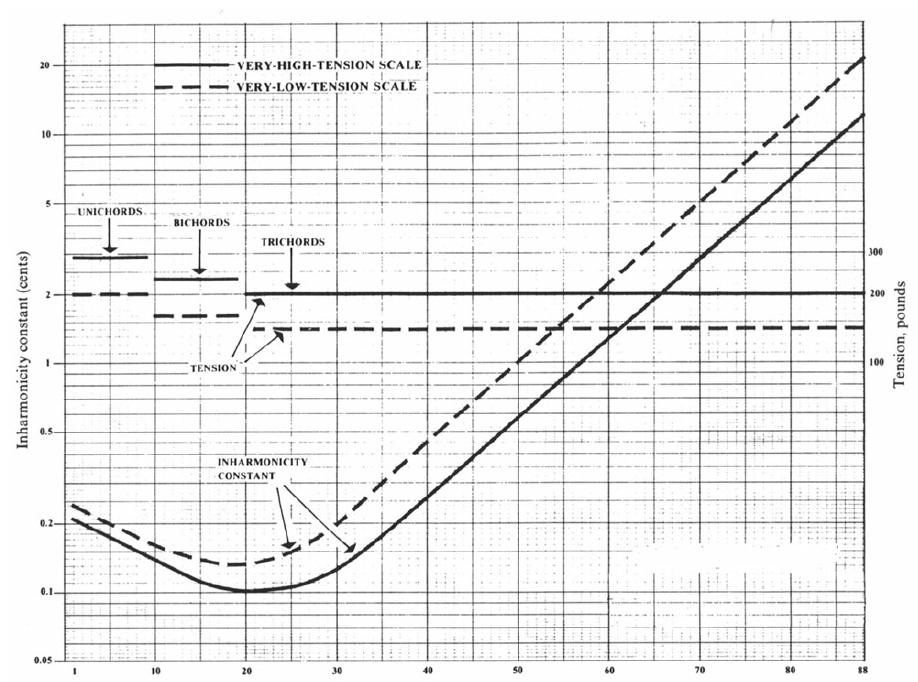
\includegraphics[width=0.6\linewidth]{00_Images/02_chapter/img147.jpg}
\caption{Typical string-scale trends along the keyboard: tension and inharmonicity evolution}
\label{fig:string_scales_trends}
\end{figure}

\subsection{Stiff-string Partials and Inharmonicity} 

For a pinned stiff string, the \( n \)-th partial can be expressed as
\[
f_n = n f_1 \left[\frac{1+n^{2}B}{1+B}\right]^{1/2}
\]
where \( B \) is the inharmonicity coefficient. A representative value for piano strings is
\[
B = 0.0004
\]
With this value, the \( 17 \)-th partial is shifted by about one partial position, namely close to the frequency of the \( 18 \)-th partial of an ideal flexible string. The inharmonicity can be expressed in cents as
\[
I_n = 1200\log_2\left[1+n^{2}B\right]^{1/2} \approx 866\,n^{2}B = b n^{2}
\]
where
\[
b = 866 B
\]

\subsection{Variation Along the Scale} 

Piano string scales show a systematic variation of tension and inharmonicity with note number. The reported trend highlights that different design choices (for instance very-high-tension versus very-low-tension scales) lead to different inharmonicity levels across the keyboard, while keeping the overall musical compass.

\subsection{Transmission-line Representation} 

Strings can be modeled by electrical transmission lines. Mass and compliance per unit length are represented by inductance and capacitance per unit length, respectively, while the transverse displacement is represented by current. In this analogy, the hammer can be represented by an inductance with a voltage across its terminals, and different switch configurations describe the contact condition between hammer and string. A transmission-line representation of the string and its coupling to excitation/termination is shown in figure \ref{fig:string_transmission_line_model}.

\begin{figure}[!htb]
\centering
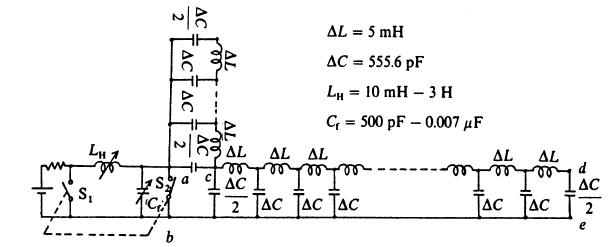
\includegraphics[width=0.8\linewidth]{00_Images/02_chapter/img162.jpg}
\caption{Transmission-line model of the string with excitation and termination elements}
\label{fig:string_transmission_line_model}
\end{figure}

\section{Piano Hammers}

Piano hammers are typically made of a hardwood core covered by one or two layers of felt. Modern bass hammers are larger than treble ones, so typical hammer masses range from about \SI{10}{\gram} in the bass down to about \SI{3.8}{\gram} in the treble. The felt covering is a key element in determining the tone.

\begin{itemize}
    \item The thickness of the outer felt layer increases from treble to bass, and its density is typically in the range
    \[
    \rho_f \in \SIrange{0.6}{0.7}{\gram\per\centi\meter\cubed}
    \]
    \item Hard hammers tend to produce a brilliant but potentially harsh sound, while soft hammers produce a duller tone.
\end{itemize}

A crucial point is that felt does not behave as a linear spring. Instead of Hooke's law, a nonlinear relation is used,
\[
F = K \xi^{p}
\]
where \( \xi \) is the compression. For used hammers, the exponent is typically in the range
\[
p \in \SIrange{2.2}{3.5}{}
\]
while for unused hammers it is often smaller,
\[
p \in \SIrange{1.5}{2.8}{}
\]
Moreover, \( K \) and \( p \) may differ between compression and relaxation, resulting in hysteresis. An important consequence of this nonlinearity is that the felt is effectively harder at high impact velocity than at low velocity, which contributes to a brighter sound at stronger dynamics. The striking point and the hammer mass influence the spectral envelope of the excited string motion. If an idealized hammer strikes the string at a fraction \( \beta \) of the string length, harmonics for which the striking point coincides with a node are strongly attenuated. This is consistent with the standard dependence of harmonic amplitudes on the factor \( \sin(n\pi\beta) \), which vanishes when \( n\beta \) is an integer. If the hammer mass is not negligible compared to the string mass, the spectrum shows a progressively stronger high-frequency roll-off above a certain partial number. For heavier hammers, the hammer may remain in contact with the string long enough for several reflected pulses to return, attenuating the motion and reducing clarity. Computer simulations indicate that, for a hard hammer, the high-frequency energy spectrum envelope can exhibit an approximate slope of \SI{-6}{\decibel} per octave. For treble strings, where the hammer mass can exceed the string mass, the slope may reach about \SI{-12}{\decibel} per octave. Experimental waveforms illustrate that hammer-string contact time must be interpreted relative to the fundamental period, and that reflections from the agraffe may appear as distinct features in the measured string velocity. Representative waveforms and spectra for different registers, together with typical contact-time values, are shown in figure \ref{fig:waveforms_spectra_contact_time}.

\begin{figure}[!htb]
\centering
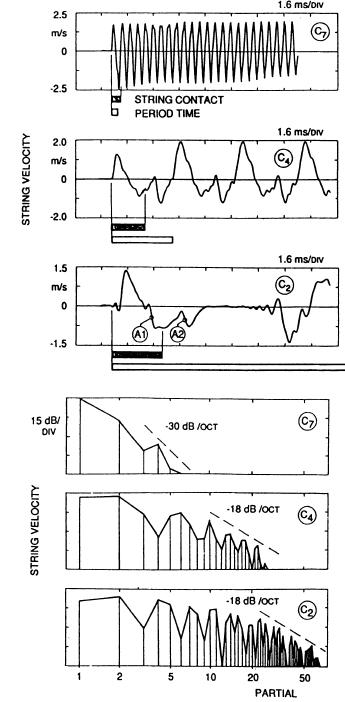
\includegraphics[width=0.6\linewidth]{00_Images/02_chapter/img190.jpg}
\caption{Waveforms and spectra for different registers and corresponding contact-time indications}
\label{fig:waveforms_spectra_contact_time}
\end{figure}

\subsection{Voicing}

Voicing is the set of operations used to adjust hammer hardness, its gradient, and related properties in order to obtain a desired tone. Typical interventions are the following:

\begin{itemize}
    \item If the hammer is too soft, it can be hardened by removing soft felt or by chemical hardening processes.
    \item If the hammer is too hard, it can be softened by piercing the felt with needles.
\end{itemize}

Voicing is typically applied differently depending on the desired dynamic range, with distinct regions of the hammer surface associated with loud, medium, and soft playing. The qualitative effect of hammer voicing on tone color is summarized in figure \ref{fig:hammer_voicing} and the influence of hammer hardness on the radiated spectrum is illustrated in figure \ref{fig:hammer_hardness_spectra}.

\begin{figure}[!htb]
\centering
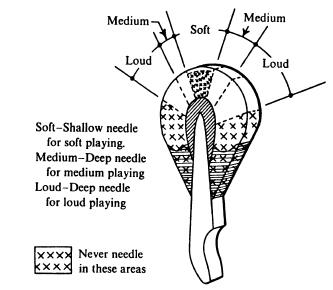
\includegraphics[width=0.6\linewidth]{00_Images/02_chapter/img204.jpg}
\caption{Hammer voicing and its influence on spectral balance across playing levels}
\label{fig:hammer_voicing}
\end{figure}

\begin{figure}[!htb]
\centering
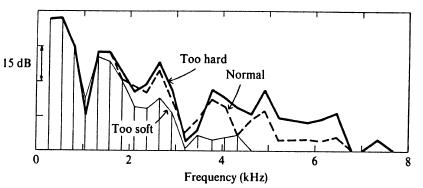
\includegraphics[width=0.7\linewidth]{00_Images/02_chapter/img223.jpg}
\caption{Effect of hammer hardness on the spectrum for a representative note}
\label{fig:hammer_hardness_spectra}
\end{figure}

\subsection{Striking Point Ratio}

Let \( d \) be the distance between the agraffe and the hammer contact point, and \( L \) the total string length. The ratio \( d/L \) is a relevant design parameter. In modern pianos, the ratio \( d/L \) is more constant along the keyboard than in older instruments. The choice of striking point reflects a compromise between fundamental strength and tone quality.

\begin{itemize}
    \item Reducing \( d/L \) tends to make the sound thinner because the fundamental becomes weaker.
    \item Too large a ratio can reduce clarity because the hammer dwell time becomes excessive.
\end{itemize}

Typical striking-point ratios along the keyboard, and their historical evolution, are shown in figure \ref{fig:striking_point_ratio}.

\begin{figure}[!htb]
\centering
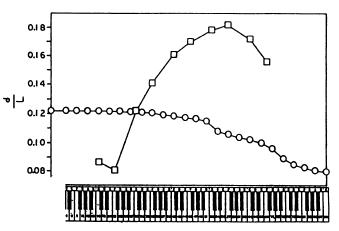
\includegraphics[width=0.7\linewidth]{00_Images/02_chapter/img238.jpg}
\caption{Striking point ratio along the keyboard for historical and modern designs}
\label{fig:striking_point_ratio}
\end{figure}

\section{Sound Board}

The soundboard of the piano is made of glued strips of spruce. Under the board, ribs run in the cross-grain direction: their main role is to stiffen the soundboard across the grain, bringing the cross-grain stiffness closer to the along-grain one. The soundboard has two distinct functions:

\begin{itemize}
    \item A static function: it must bear the load transferred from strings and bridges, typically between \SI{900}{\newton} and \SI{1800}{\newton}.
    \item An acoustic function: it is the main radiating component of the instrument and it converts vibrational energy coming from bridges and strings into acoustic energy.
\end{itemize}

Modern pianos have two bridges, a main (treble) bridge and a bass bridge. The bass bridge is typically \SIrange{2}{3}{\centi\meter} taller than the treble bridge, so that bass strings can pass over the treble ones. Bridges act as impedance transformers: they present to the strings an input impedance much higher than the one that would be obtained if strings were attached directly to the soundboard. Moreover, bridges enable the soundboard to respond to string vibration both normal to the board and in the plane of the board, including contributions associated with longitudinal string motion.

\subsection{Treble and Bass Bridges}

The relative placement of bass and treble bridges is arranged to accommodate overlapping string groups and to drive the soundboard over a large region, rather than concentrating excitation close to one edge. The treble and bass bridges and their placement on the soundboard are shown in figure \ref{fig:treble_bass_bridges}.

\begin{figure}[!htb]
\centering
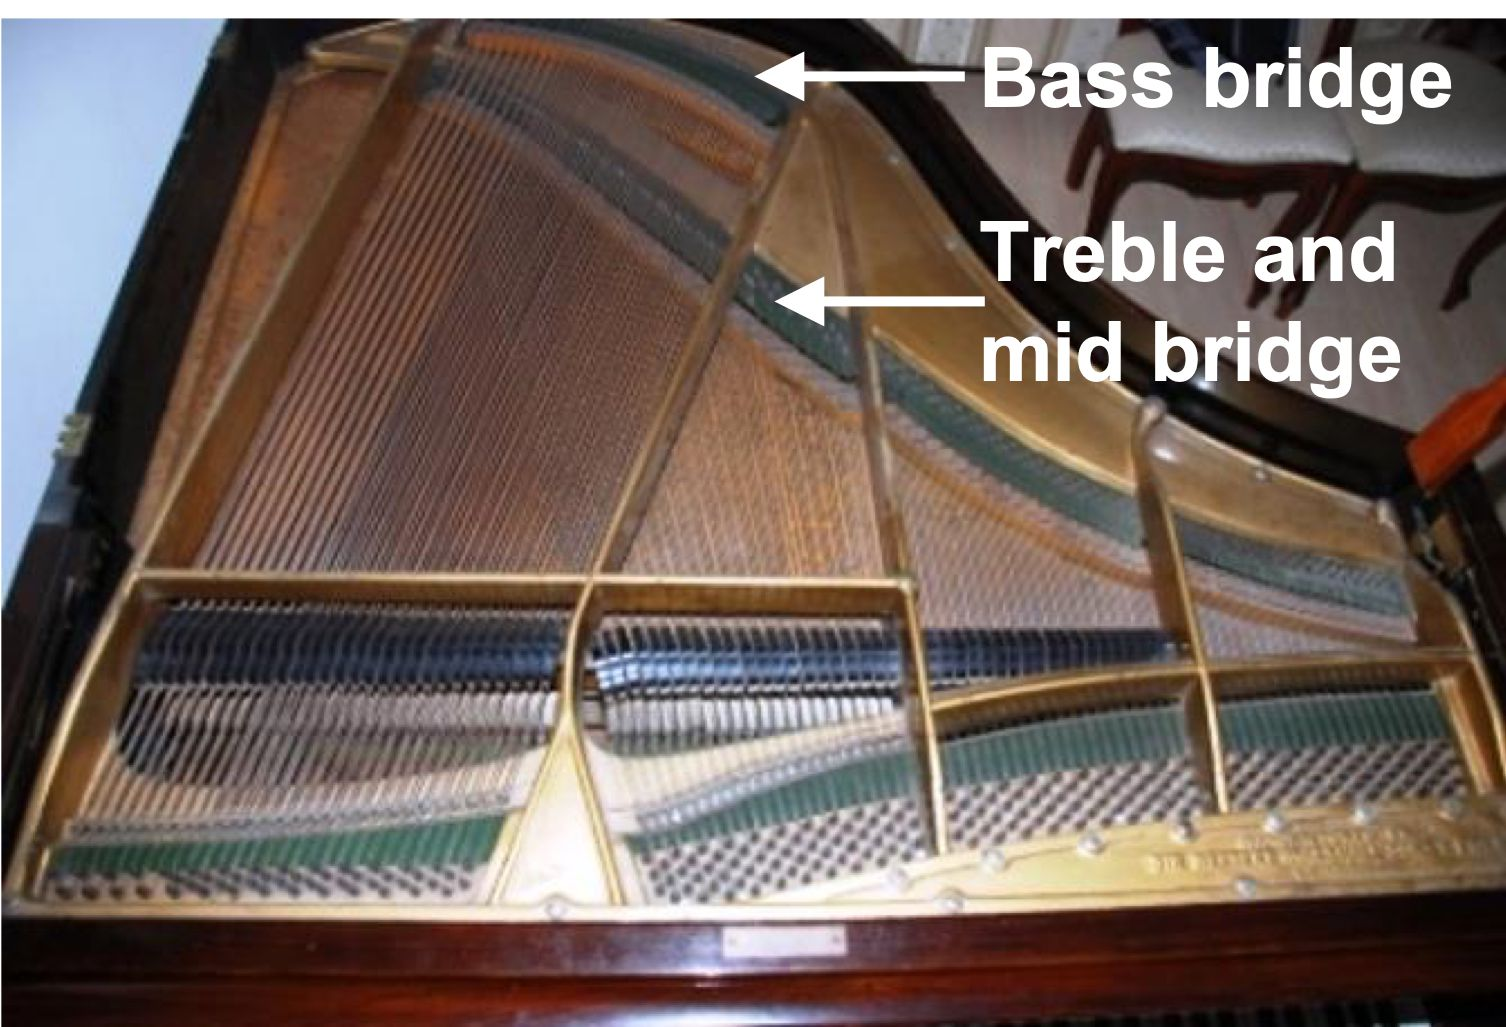
\includegraphics[width=0.7\linewidth]{00_Images/02_chapter/img249.jpg}
\caption{Treble and bass bridges on the piano soundboard}
\label{fig:treble_bass_bridges}
\end{figure}

\subsection{Cantilevered Bridges}

In small pianos, bridges may be cantilevered to shift the soundboard driving point away from the stiff perimeter zone while still allowing the longest possible string lengths. The cantilever region separates the string-bridge attachment point from the bridge-board attachment point, so that the board is driven more effectively in its vibratory area. A schematic representation of cantilevered bridge solutions is shown in figure \ref{fig:cantilevered_bridges}.

\begin{figure}[!htb]
\centering
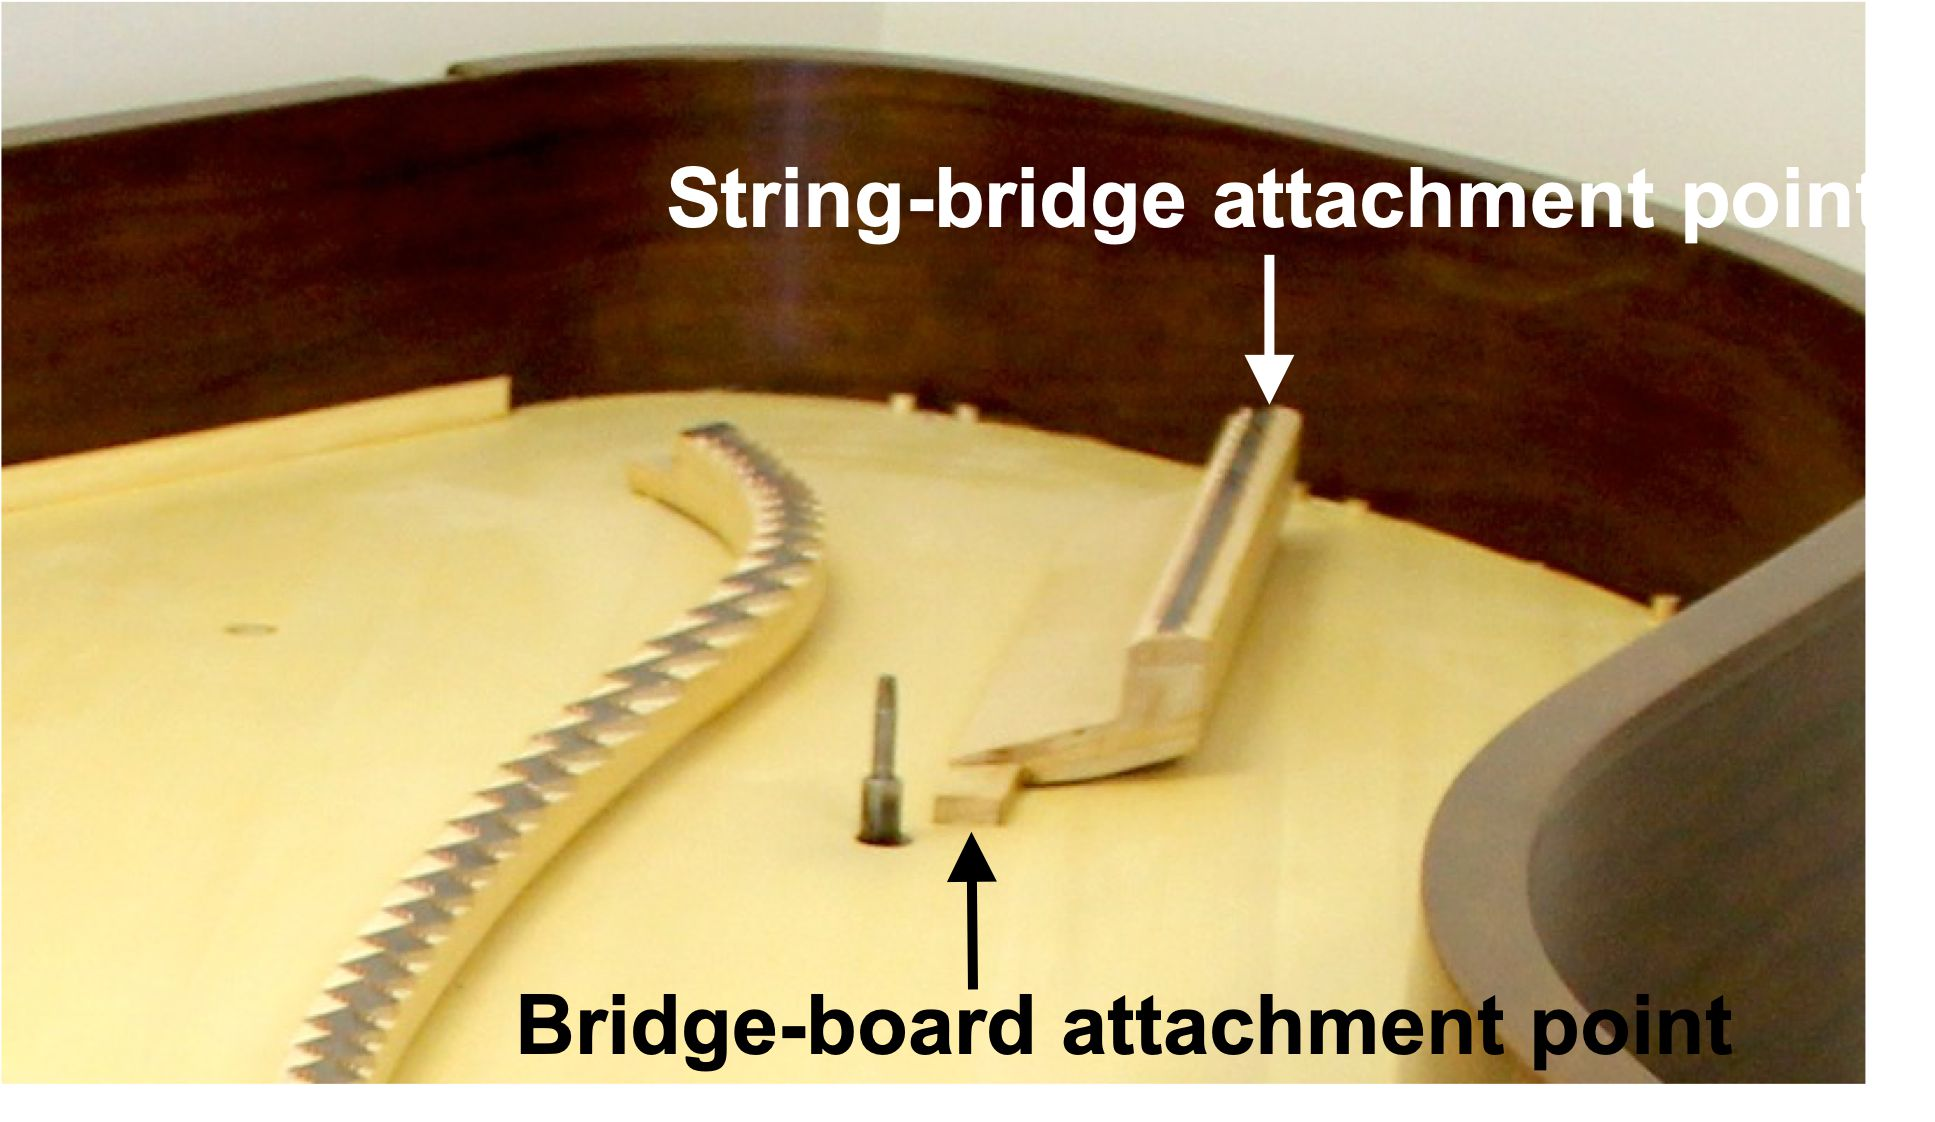
\includegraphics[width=0.7\linewidth]{00_Images/02_chapter/img256.jpg}
\caption{Cantilevered bridge concept for string-to-soundboard coupling}
\label{fig:cantilevered_bridges}
\end{figure}

\subsection{Sound Board}

For an upright piano, the soundboard can be idealized as a rectangular plate on which the treble and bass bridges are mounted. Trimming rims delimit the area effectively subject to vibration to an approximately trapezoidal region, while bridges run diagonally across it. This geometry is useful when comparing measurements performed on a simplified rectangular board without trimming rims. An upright soundboard and its simplified rectangular representation used for measurements are shown in figure \ref{fig:upright_soundboard_rectangular}.

\begin{figure}[!htb]
\centering
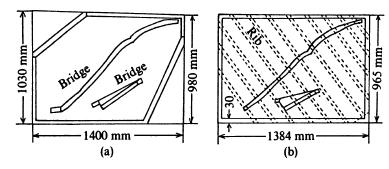
\includegraphics[width=0.7\linewidth]{00_Images/02_chapter/img271.jpg}
\caption{Upright soundboard and simplified rectangular representation for modal studies}
\label{fig:upright_soundboard_rectangular}
\end{figure}

Chladni figures measured on a rectangular soundboard illustrate the progression of mode shapes with frequency. Examples of Chladni patterns measured on a simplified soundboard are shown in figure \ref{fig:chladni_patterns_soundboard}.

\begin{figure}[!htb]
\centering
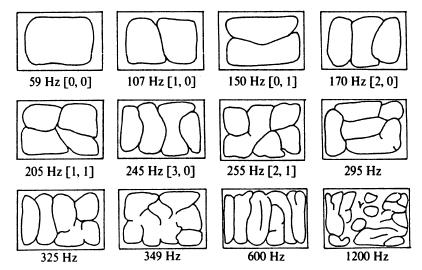
\includegraphics[width=0.7\linewidth]{00_Images/02_chapter/img285.jpg}
\caption{Chladni figures illustrating soundboard mode shapes}
\label{fig:chladni_patterns_soundboard}
\end{figure}

Low-order patterns can be associated with modal indices \( (m,n) \), for instance around
\[
\SI{59}{\hertz}\ (0,0), \quad \SI{107}{\hertz}\ (1,0), \quad \SI{150}{\hertz}\ (0,1), \quad \SI{170}{\hertz}\ (2,0), \quad \SI{205}{\hertz}\ (1,1)
\]
with increasingly complex nodal structures at higher frequencies, for example around \SI{600}{\hertz} and \SI{1200}{\hertz}. The observed modal frequencies lie between those expected for a board with clamped edges and a board with hinged edges. Since the bridge extends over a relevant fraction of the board length, the driving-point impedance measured on the bridge is expected to depend on the measurement location. A set of bridge points can be associated with the fundamental frequencies of the corresponding strings, spanning from low notes in the bass to very high notes in the treble. The measurement locations along the bridges, referenced to the corresponding string fundamentals, are shown in figure \ref{fig:bridge_measurement_points}. As a consequence, the mechanical impedance encountered by different string groups is not uniform along the bridge. Driving-point impedance measurements at different bridge locations show that minima of impedance often occur near the fundamental frequencies of the corresponding notes, which is a desirable feature for energy transfer and tonal balance. It is also observed that, above about \SI{1000}{\hertz}, the decrease of driving-point impedance is not particularly rapid in a grand piano. This behavior is often indicated as one reason for acoustic differences between grand and upright instruments. Radiation efficiency is strongly frequency dependent. Below the critical frequency of the soundboard, radiation efficiency drops because bending waves produce evanescent acoustic fields. Above a certain frequency, radiation resistance increases and can approach the characteristic impedance of air, although internal losses limit the effective radiation efficiency at high frequency. As a practical consequence, the frequency region that is favored for acoustic radiation is typically between \SI{200}{\hertz} and \SI{2000}{\hertz}. Driving-point impedance measured at different bridge locations is shown in figure \ref{fig:driving_point_impedance_locations}.

\begin{figure}[!htb]
\centering
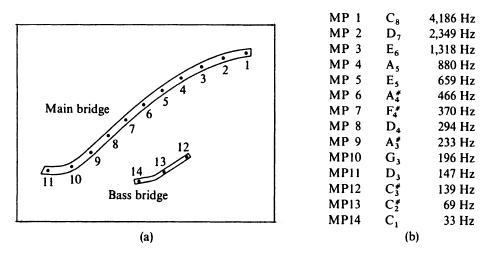
\includegraphics[width=0.65\linewidth]{00_Images/02_chapter/img299.jpg}
\caption{Bridge measurement points and corresponding string fundamental frequencies}
\label{fig:bridge_measurement_points}
\end{figure}

\begin{figure}[!htb]
\centering
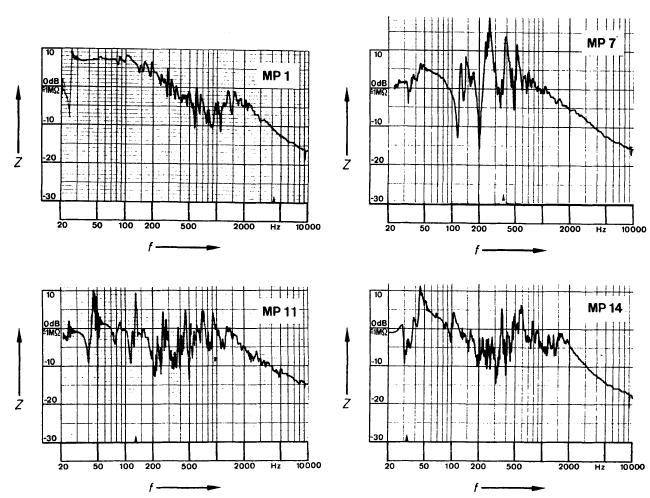
\includegraphics[width=0.65\linewidth]{00_Images/02_chapter/img313.jpg}
\caption{Driving-point impedance at different points along the bridge}
\label{fig:driving_point_impedance_locations}
\end{figure}

A comparison between the driving-point impedance and the radiated sound shows that impedance peaks do not always coincide with the dominant peaks in the radiated spectrum. One reason is that efficient radiation requires bending-wave speeds at those frequencies to be close to the speed of sound in air, which is satisfied only in a band near the critical frequency. Internal damping broadens this band and smooths the correspondence between mechanical peaks and radiated peaks. Overall radiation efficiency is affected by several factors, among which the position of the lid in a grand piano plays a relevant role. A representative comparison between mechanical impedance trends and radiated sound is shown in figure \ref{fig:impedance_vs_radiation}.

\begin{figure}[!htb]
\centering
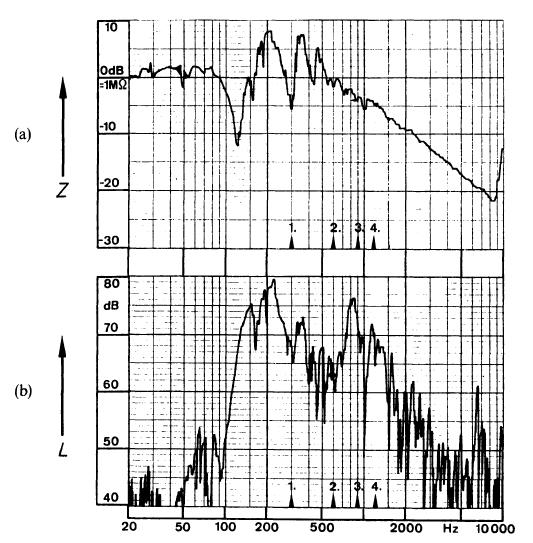
\includegraphics[width=0.6\linewidth]{00_Images/02_chapter/img329.jpg}
\caption{Comparison between driving-point impedance behavior and radiated sound level trends}
\label{fig:impedance_vs_radiation}
\end{figure}

Radiation patterns in a vertical plane show increased radiation over a range of angles when the lid is open. At low frequency it is desirable to increase bending-wave speed to improve radiation efficiency. This is attained by stiffening the board through ribs, while keeping the corresponding mass increase as small as possible. Since rib stiffness increases approximately with the square of rib height while rib mass is approximately proportional to height, a practical guideline is to use ribs that are narrow and high. Measured radiation patterns for different registers and lid configurations are shown in figure \ref{fig:radiation_patterns_lid_register}.

\begin{figure}[!htb]
\centering
\subfloat{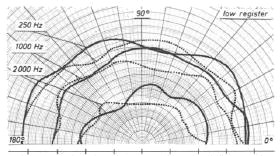
\includegraphics[width=0.3\linewidth]{00_Images/02_chapter/img349_1.jpg}}\hfill
\subfloat{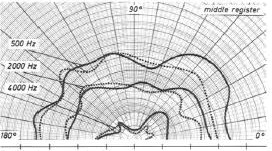
\includegraphics[width=0.3\linewidth]{00_Images/02_chapter/img349_2.jpg}}\hfill
\subfloat{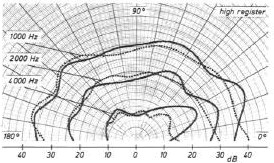
\includegraphics[width=0.3\linewidth]{00_Images/02_chapter/img349_3.jpg}}
\caption{Radiation patterns for different registers with lid open and closed}
\label{fig:radiation_patterns_lid_register}
\end{figure}

Sound levels across the full keyboard depend on playing force and illustrate that the radiated output varies substantially with register and excitation strength. The vibrational and radiative properties of a grand piano are markedly different from those of other piano types, particularly at low frequency. Overall sound levels across the full keyboard for different playing forces are shown in figure \ref{fig:sound_levels_88_notes}.

\begin{figure}[!htb]
\centering
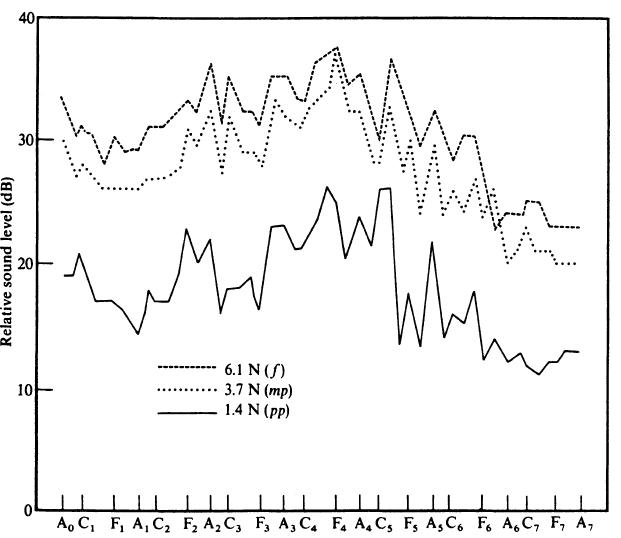
\includegraphics[width=0.55\linewidth]{00_Images/02_chapter/img367.jpg}
\caption{Sound levels across the 88 keys for different playing forces}
\label{fig:sound_levels_88_notes}
\end{figure}

Frequency responses obtained by exciting the soundboard at multiple points show that a small number of low-frequency modal peaks are consistently present in the measured spectra, and corresponding mode shapes can be identified. In addition, radiation efficiency can be large at several frequencies that are not at or near structural resonances. Two mechanisms are highlighted: cancellation of sound from different vibrating areas of the soundboard surface, and large volume velocity arising when two modes interfere strongly. Finally, when strings are mounted, the mobility (velocity/force) normal to the soundboard at bridge termination points decreases by about \SIrange{10}{15}{\decibel}. This is attributed to the high tension introduced by the strings, which limits soundboard mobility in the normal direction. A representative set of soundboard response spectra is shown in figure \ref{fig:soundboard_frequency_response}. Modal peaks and the link to corresponding mode shapes are summarized in figure \ref{fig:modal_peaks_mode_shapes}. Examples of soundboard mode shapes are shown in figure \ref{fig:soundboard_mode_shapes_1}. Additional mode-shape examples are shown in figure \ref{fig:soundboard_mode_shapes_2}.

\begin{figure}[!htb]
\centering
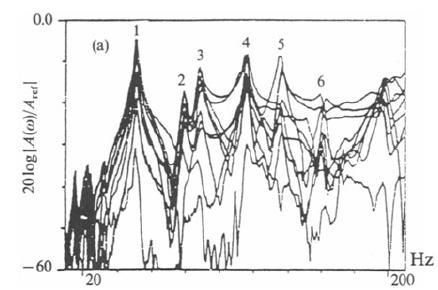
\includegraphics[width=0.55\linewidth]{00_Images/02_chapter/img381.jpg}
\caption{Soundboard frequency response showing multiple spectra overlaid}
\label{fig:soundboard_frequency_response}
\end{figure}

\begin{figure}[!htb]
\centering
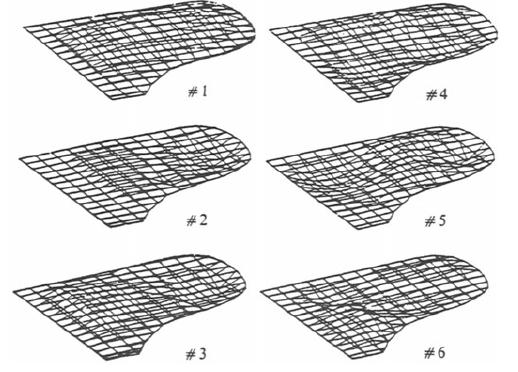
\includegraphics[height=0.27\textheight]{00_Images/02_chapter/img395.jpg}
\caption{Modal peaks in the response and corresponding mode-shape indications}
\label{fig:modal_peaks_mode_shapes}
\end{figure}

\begin{figure}[!htb]
\centering
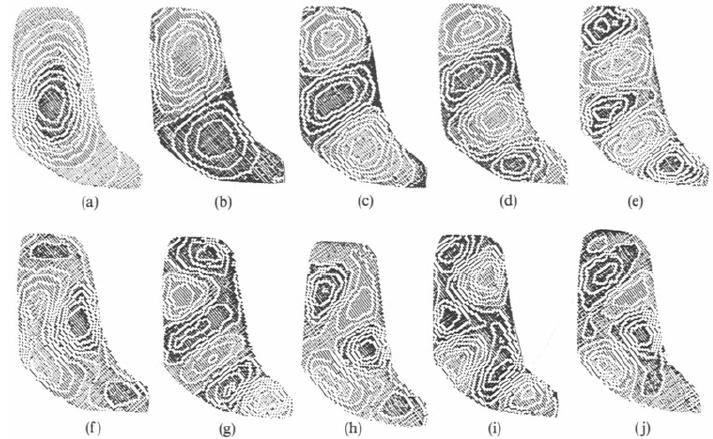
\includegraphics[height=0.27\textheight]{00_Images/02_chapter/img409.jpg}
\caption{Examples of soundboard mode shapes at selected resonant frequencies}
\label{fig:soundboard_mode_shapes_1}
\end{figure}

\begin{figure}[!htb]
\centering
\subfloat{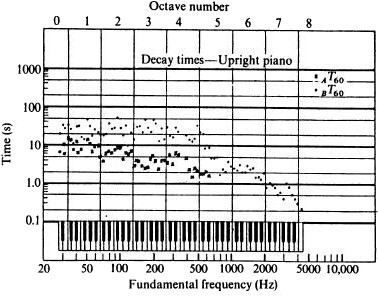
\includegraphics[width=0.45\linewidth]{00_Images/02_chapter/img435_1.jpg}}\hfill
\subfloat{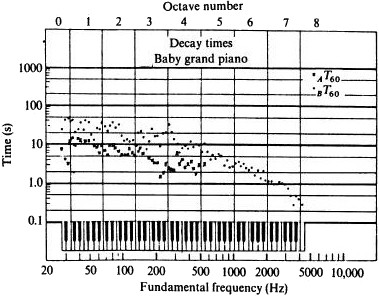
\includegraphics[width=0.45\linewidth]{00_Images/02_chapter/img435_2.jpg}}
\caption{Additional soundboard mode shapes illustrating the modal family over frequency}
\label{fig:soundboard_mode_shapes_2}
\end{figure}

\section{Sound Decay}

\subsection{Compound Decay and Decay Times}

The envelope of a piano tone typically exhibits a compound decay: an initial portion with a relatively high decay rate, followed by a second portion with a slower decay. Two phenomena are mainly responsible for this behavior: the change of polarization of the string motion during vibration and the coupling among strings within an unison group. To describe the decay in a compact way, two time measures are introduced:

\begin{itemize}
    \item \( AT_{60} \) is the reverberation time that would be observed if the faster initial decay continued unchanged.
    \item \( BT_{60} \) is the decay time associated with the overall tone, including the slower second part.
\end{itemize}

An example of compound decay and the definition of decay-time descriptors is shown in figure \ref{fig:compound_decay_AT_BT}.

\begin{figure}[!htb]
\centering
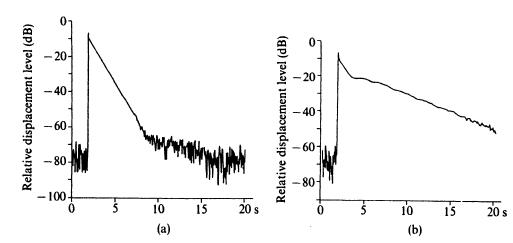
\includegraphics[width=0.7\linewidth]{00_Images/02_chapter/img454.jpg}
\caption{Compound decay and definition of \(AT_{60}\) and \(BT_{60}\)}
\label{fig:compound_decay_AT_BT}
\end{figure}

\subsection{Polarization-dependent Coupling to the Soundboard}

The soundboard impedance is not the same for different directions of string motion at the bridge. In particular, the impedance encountered for horizontal vibration is greater than for vertical vibration, because the soundboard is typically stiffer to tangential displacement than to orthogonal displacement. This difference can be observed by comparing decay curves measured on a single string, for instance for a \( D \sharp 4 \) string with fundamental frequency \( f=\SI{311}{\hertz} \), where the decay is markedly different for perpendicular and parallel polarizations. Polarization-dependent decay behavior for a representative note is shown in figure \ref{fig:polarization_dependent_decay}.

\begin{figure}[!htb]
\centering
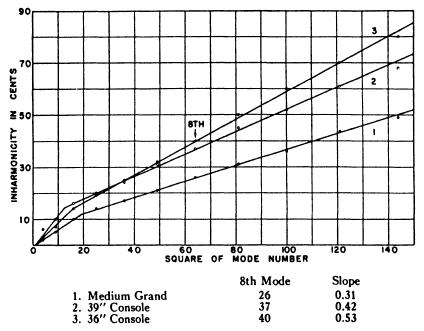
\includegraphics[width=0.6\linewidth]{00_Images/02_chapter/img469.jpg}
\caption{Decay curves for perpendicular and parallel polarizations of string motion}
\label{fig:polarization_dependent_decay}
\end{figure}

\subsection{Depolarization Mechanism During a Note}

When the hammer strikes the strings, the initial vibration polarization is mainly vertical. In the early stage of the note, the dominant impedance mismatch is therefore that between the string and the soundboard response to vertical displacement. For most strings, the spiral-like winding induces a net transfer of energy from the vertical polarization to the horizontal one. Since the vertical and horizontal displacements are out of phase, the motion can evolve toward a circular polarization. During the second part of the vibration, energy is then transmitted to the bridge also through the horizontal component. Because the mismatch between the string impedance and the soundboard impedance is much greater for horizontal than for vertical displacements, the energy transfer rate becomes smaller as the motion depolarizes. As a result, the tone tends to start with a rapid decay and then slow down over time.

\subsection{Unison Coupling and Phase Dispersion}

In unison groups, when the hammer strikes, the strings start vibrating approximately in phase. They therefore transfer energy to the soundboard in phase, which increases the effective transfer rate and contributes to the faster initial decay. Due to small tuning differences, after a few vibration cycles the strings gradually get out of phase. The resulting reduction in coherent energy transfer decreases the decay rate, producing a longer-lasting second part of the note. This depolarization-related effect can also be exploited in tuning practice to influence the perceived length of the aftersound.

\section{Tuning and Inharmonicity}

\subsection{Octave Stretching}

In a tuned piano, octaves are slightly stretched with respect to the ideal \( 2:1 \) frequency ratio, so that the octave note is set a bit higher than \( 2f \). There are two main reasons for adopting this practice.

\paragraph{Inharmonicity and beat reduction} Because of string stiffness, partials are stretched upward with respect to integer multiples of the fundamental. As a consequence, if an exact \( 2:1 \) octave is enforced, upper partials of the lower note can fall close to prominent partials of the upper note and produce audible beating. A slight octave stretch reduces such beats by improving the coincidence between relevant partials across the octave. This effect is stronger for short strings, which tend to exhibit larger inharmonicity. For this reason, octave stretching is typically more pronounced in upright pianos than in grand pianos.

\paragraph{Psychoacoustic motivation} A second contribution is perceptual: when two notes are several octaves apart, listeners tend to judge them as being in tune when a certain amount of stretch is present. For example, if a melody is about two octaves higher than the accompaniment, a stretching on the order of a semitone may be needed for the interval to be perceived as correctly tuned.

\subsection{Comparison Across Different Pianos}

A comparison of inharmonicity expressed in cents shows that smaller instruments generally exhibit higher inharmonicity than larger ones. The reported plot of inharmonicity versus the square of the mode number displays steeper trends for console pianos than for a medium grand, consistent with the stronger stiffness effects expected for shorter strings.


    %! TEX rootmain.tex

\chapter{Violin}

The violin is a bowed-string instrument in which sustained excitation is provided by frictional interaction between bow and strings. The string motion is transmitted to the body through the bridge, and the vibrating structure radiates sound through a combination of structural and air-coupled mechanisms. Following the course outline, the discussion starts from the instrument anatomy and then moves to historical notes, bowed-string motion, body vibrations and transient response, internal components such as soundpost and bass bar, the bridge and its coupling to the soundboard, sound radiation, wolf notes, and electrical analog models.

\section{Anatomy of the Violin}

A reference view of the violin and its main components is shown in figure \ref{fig:violin_anatomy}.

\begin{figure}[!htb]
\centering
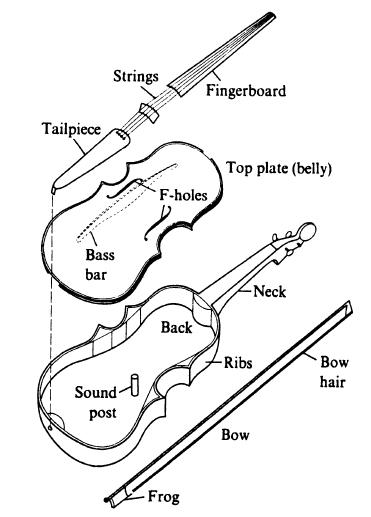
\includegraphics[width=0.6\linewidth]{00_Images/03_chapter/img53.jpg}
\caption{Anatomy of the violin and main components}
\label{fig:violin_anatomy}
\end{figure}

\subsection{Main Components and Materials}

A violin can be described by its strings, the carved wooden body, and a small set of internal components that strongly influence vibration transfer. The strings are typically steel, gut, or nylon, tuned to \( G_3 \), \( D_4 \), \( A_4 \), and \( E_5 \). The top plate is commonly carved from spruce, such as Picea abies or Picea excelsis, while back, ribs, and neck are commonly made from maple, such as Acer platanoides. The fingerboard is made from ebony and the bow stick from Pernambuco. Under the top plate, the bass bar provides local stiffening. The soundpost is positioned near the treble foot of the bridge and provides a mechanical coupling between top and back plates. 

\subsection{Geometry, Thicknesses, and Static Loads}

Typical violin dimensions are about \SI{35}{\centi\meter} in body length, with upper and lower bout widths of about \SIrange{16}{20}{\centi\meter}. Ribs are about \SIrange{30}{32}{\milli\meter} high. Plate thickness varies across the instrument. Representative values are \SIrange{2.0}{3.5}{\milli\meter} for the top plate and \SIrange{2.0}{6.0}{\milli\meter} for the back, while the maximum arch height of both plates is about \SI{15}{\milli\meter}. Exact thickness and arching depend on the violin-maker choices and on the vibroacoustic behavior of the specific wood piece. On the top plate, a channel is cut along the edge and filled with strips of wood called purfling. This detail promotes a boundary behavior closer to hinged than clamped, allowing larger plate mobility near the edge. The total string tension is about \SI{220}{\newton}. The resulting downward force on the bridge is about \SI{90}{\newton}, supported by the arching and internally by the bass bar and the soundpost.

\subsection{Sound Production in Brief}

Sound production can be summarized as a short chain of coupled events:

\begin{itemize}
    \item The violinist draws the bow across the strings, setting them into vibration.
    \item The vibrating strings exert forces on the bridge and excite the body motion.
    \item The body vibration produces acoustic radiation.
\end{itemize}

While the sequence appears simple, many subtleties are hidden in the excitation and in the coupled structural response, which is why the violin is among the most studied musical instruments. 

\section{Motion of Bowed Strings}

In bowed-string excitation, the frictional interaction between bow and string produces a stick-slip motion that generates one or more traveling bends. These bends run around a curved envelope, whose maximum amplitude depends on the bow speed and on the bowing position. Bowing at a single point divides the string into two segments. The basic kinematics of bowed-string motion, including sticking and slipping phases, is summarized in figure \ref{fig:bowed_string_motion_basic}.

\begin{figure}[!htb]
\centering
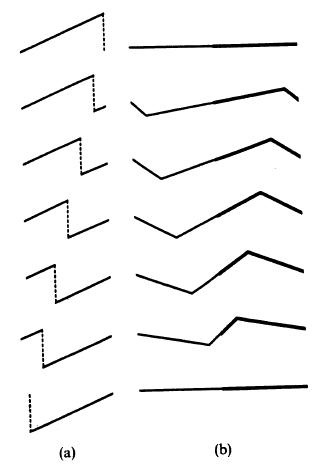
\includegraphics[width=0.6\linewidth]{00_Images/03_chapter/img80.jpg}
\caption{Basic description of bowed-string motion over a cycle}
\label{fig:bowed_string_motion_basic}
\end{figure}

If \( x_b \) is the distance from the bridge to the bowing point and \( L \) is the string length, the segment lengths are in the ratio
\[
\frac{L-x_b}{x_b} = p
\]
The resulting velocity pattern can be interpreted as the superposition of a positive and a negative traveling wave of the same form. When the two waves are coincident, the velocity diagram becomes a straight line passing through one end of the string, with a discontinuity at the other. A modal representation of the transverse displacement is
\[
y(x,t) = \sum_{n = 1}^{\infty} a_n \sin\left(\frac{n\pi x}{L}\right)\sin(n\omega t)
\]
In inappropriate bowing conditions, in particular when the bowing force is not sufficient in relation to the bowing position, more than a single bend can be generated. This may lead to double-slip or multiple-flyback regimes, producing force waveforms at the bridge that differ markedly from the regular Helmholtz motion. Examples of non-ideal periodic regimes such as double-slip and multiple-flyback motion are shown in figure \ref{fig:bowed_string_nonideal}.

\begin{figure}[!htb]
\centering
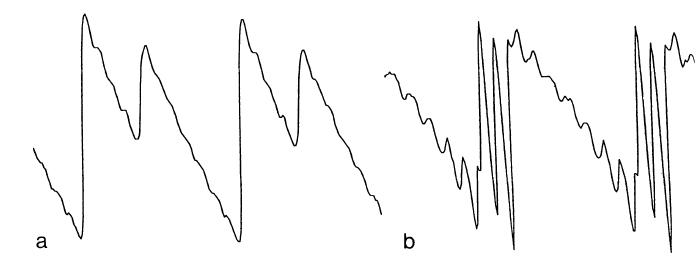
\includegraphics[width=0.7\linewidth]{00_Images/03_chapter/img105.jpg}
\caption{Non-ideal bowed-string regimes: double slip and multiple flyback}
\label{fig:bowed_string_nonideal}
\end{figure}

Louder playing requires both higher bow speed and bowing closer to the bridge. A compact estimate links these parameters to the maximum displacement and to the maximum transverse force at the bridge,
\[
y_m = \frac{1}{8f}\frac{v_b}{x_b}
\]
\[
F_m = \mu c \frac{v_b}{x_b}
\]
where \( v_b \) is the bowing speed, \( f \) is the playing frequency, \( \mu \) is the string mass per unit length, and \( c \) is the transverse wave speed. Due to string stiffness, the Helmholtz corner is not perfectly sharp. Two consequences are commonly observed: the pitch can flatten as bow force increases, and the period can show jitter, with variations up to about \SI{30}{cent} between minimum and maximum values. Besides transverse motion, bowed strings can support additional wave types. Longitudinal vibrations generate sounds that are not harmonically related to the transverse partials. Representative longitudinal-mode frequencies are around \SI{1350}{\hertz} and \SI{2700}{\hertz} for the \( G \) and \( D \) strings. Torsional waves are also excited by the bowing action, with propagation speed
\[
c_T = \sqrt{\frac{G K_T}{\rho I}}
\]
where \( G \) is the shear modulus, \( K_T \) is a torsional stiffness factor, \( \rho \) is the density, and \( I \) is the polar moment of inertia. The ratio between torsional and longitudinal wave speeds is
\[
\frac{c_T}{c_L} = \frac{1}{\sqrt{2(1+\nu)}}
\]
It typically ranges from about \( 1/7.7 \) to \( 1/2 \), depending on the material, and torsional damping is usually much higher than transverse damping. The bow hair alone does not provide sufficient friction to trigger a stable stick-slip regime, so rosin plays a central role. Rubbing the bow with rosin deposits fragments of various sizes: larger ones tend to detach after a few strokes, while smaller ones adhere more firmly. During playing, rosin warms up, its static friction coefficient increases, and its sliding coefficient decreases. As a consequence, during slip the rosin tends to act as a lubricant, while during stick it increases bow-string friction and promotes a longer stick phase. A typical velocity-dependent friction characteristic used in dynamic bowing models is shown in figure \ref{fig:bow_friction_characteristic}.

\begin{figure}[!htb]
\centering
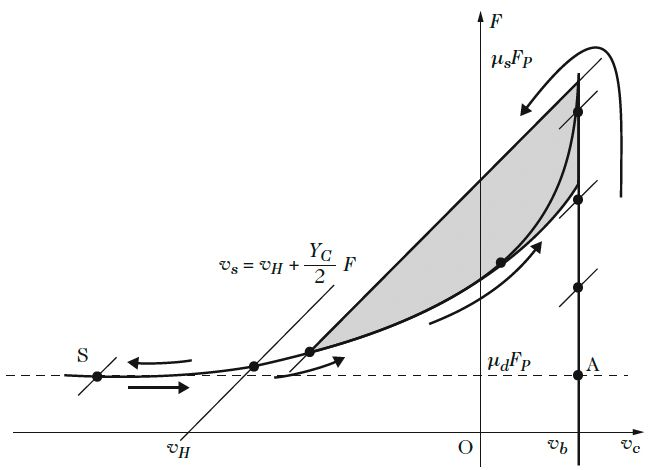
\includegraphics[width=0.7\linewidth]{00_Images/03_chapter/img127.jpg}
\caption{Velocity-dependent friction characteristic for bow-string interaction}
\label{fig:bow_friction_characteristic}
\end{figure}

\subsection{Dynamic Model}

A compact dynamic model can be written in terms of the string velocity at the bowing point \( v_s(t) \), the bow velocity \( v_b \) (assumed constant during the observation window), and the bow-string interaction force \( F(t) \),
\[
v_s(t) = \left[F \star v_{\delta}\right](t)
\]
\[
F(t) = F_{NL}\!\left[v_s(t) - v_b\right]
\]
where \( v_{\delta}(t) \) is the string velocity response to an impulsive force at the bowing point and \( F_{NL} \) is the friction curve as a function of relative velocity. It is useful to decompose the velocity as
\[
v_s(t) = v_h(t) + v_{\infty,\infty}(t)
\]
where \( v_h(t) \) is due to the history of traveling waves on the finite string and \( v_{\infty,\infty}(t) \) is due to the instantaneous action of the bow, obtained by assuming the string infinite in both directions. Introducing the characteristic admittance \( Y_c \) of an equivalent infinite string, one obtains
\[
v_{\infty,\infty}(t) = \frac{Y_c}{2}F(t)
\]
The friction law must account for different static and dynamic friction coefficients, with \( \mu_s>\mu_d \). Representative values may be \( \mu_s = 0.7 \) and \( \mu_d = 0.2 \), and experiments indicate a transition region between the two regimes. In the \( (v_s,F) \) plane, the system state is found as the intersection between the straight line
\[
v_s(t) = v_h(t) + \frac{Y_c}{2}F(t)
\]
and the friction curve. When the pressing force is small enough, the slope of the friction curve remains below \( 2/Y_c \) and only one intersection exists. When the pressing force exceeds a threshold, \( 2/Y_c \) becomes smaller than the steepest slope of the friction curve and two intersections may appear, corresponding to a sticking point and a sliding point, with the force at the sticking point larger than at the sliding point.

\subsection{Schelleng's Diagram}

For each bowing position there exists a minimum and a maximum bowing force for which the bend can trigger the beginning and end of slippage between bow and string. This is summarized by Schelleng's diagram, which provides the admissible range of bow forces as a function of the bow-to-bridge distance. As the bowing point approaches the bridge, the distance between the minimum and maximum admissible forces becomes smaller. Bowing closer to the bridge therefore requires a considerably larger and more precisely controlled force, while also leaving a reduced margin before irregular regimes such as multiple slips occur. The admissible bowing range in terms of bow force and distance from the bridge is summarized by Schelleng's diagram in figure \ref{fig:schelleng_diagram}.

\begin{figure}[!htb]
\centering
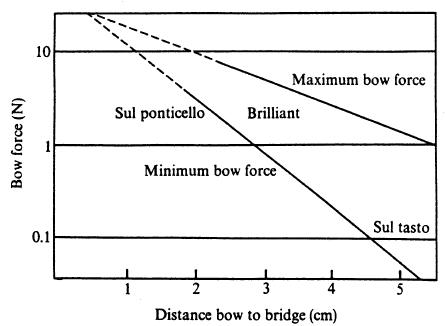
\includegraphics[width=0.7\linewidth]{00_Images/03_chapter/img144.jpg}
\caption{Schelleng's diagram for bowing limits}
\label{fig:schelleng_diagram}
\end{figure}

The combined transverse and torsional components of bowed-string motion can be visualized as in figure \ref{fig:lissajous_torsion_helmholtz}.

\begin{figure}[!htb]
\centering
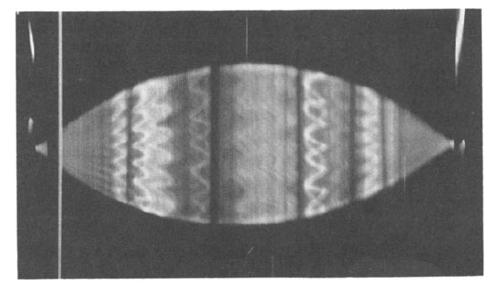
\includegraphics[width=0.7\linewidth]{00_Images/03_chapter/img159.jpg}
\caption{Lissajous representation highlighting torsional and Helmholtz components}
\label{fig:lissajous_torsion_helmholtz}
\end{figure}

\section{Violin Body Vibrations}

Violin vibrations are mainly due to the coupled motions of the top and back plates and to the enclosed air. Motions of fingerboard and ribs may be present, but they are not considered acoustically relevant in a first approximation. For modeling purposes, low-frequency behavior can be represented by a network analog, but this becomes rapidly complex because of the coupling introduced by the soundpost. For this reason, finite element modeling is often adopted to describe the vibrational response over a wider frequency range. A comparison of bridge admittance measured on different violins shows that modal frequencies vary from one instrument to another, while the overall admittance trend remains qualitatively similar. This shared trend is one of the features that makes different instruments recognizable as violins. Measured bridge admittance curves for different violins are compared in figure \ref{fig:bridge_admittance_multiple_violins}.

\begin{figure}[!htb]
\centering
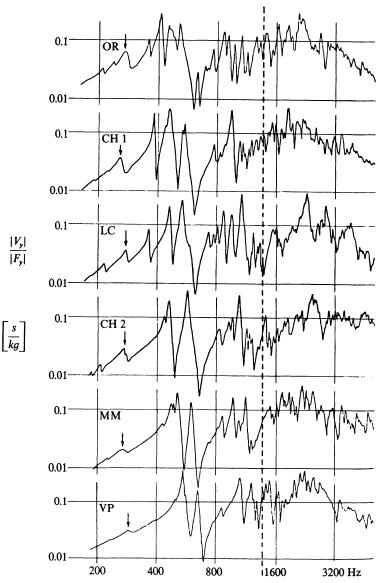
\includegraphics[width=0.5\linewidth]{00_Images/03_chapter/img174.jpg}
\caption{Bridge admittance measured on several violins}
\label{fig:bridge_admittance_multiple_violins}
\end{figure}

Even when resonance frequencies shift, modes can still be categorized according to their deformation shapes, which are comparatively invariant. Different nomenclatures exist for violin modes. In the following, mode labels are reported as \( \text{Name 1 [Name 2]} \), where the two names refer to two commonly used naming conventions.

\paragraph{Low-frequency bending modes} The mode \( C1[B^-] \) is a one-dimensional bending resembling the first bending mode of a bar. It features one nodal line near the bridge and another about halfway toward the neck, and it occurs on average around \SI{185}{\hertz}. A second bending mode (not shown) is sometimes denoted \( N \) and involves motion of neck and fingerboard. These bending-type modes are not associated with strong radiation. The first mode of major acoustical importance is the f-hole resonance \( A0[A0] \), in which a substantial amount of air moves in and out of the f-holes. It is often referred to as a Helmholtz resonance, with the caveat that the violin walls are not rigid. Its frequency is on average around \SI{275}{\hertz}. A two-dimensional flexural mode \( C2 \) is typically observed around \SI{405}{\hertz}. The mode \( T1[B1^-] \) is mainly a motion of the top plate, with average frequency around \SI{460}{\hertz}. The mode \( C3[B1^+] \) is a two-dimensional motion involving both plates and is typically around \SI{530}{\hertz}. Another important two-dimensional mode \( C4 \) occurs around \SI{700}{\hertz}. Among these, the modes designated \( A0 \), \( T1 \), \( C3 \), and \( C4 \) are often treated as the most relevant in the low-frequency range. Instruments judged best in quality tend to show a uniformly high admittance level associated with these modes. In addition, the increase in admittance between about \SIrange{1.4}{3}{\kilo\hertz}, known as the bridge hill, is commonly regarded as an important quality factor. The main low-frequency body modes (often referred to as signature modes) are illustrated in figure \ref{fig:violin_signature_modes}.

\begin{figure}[!htb]
\centering
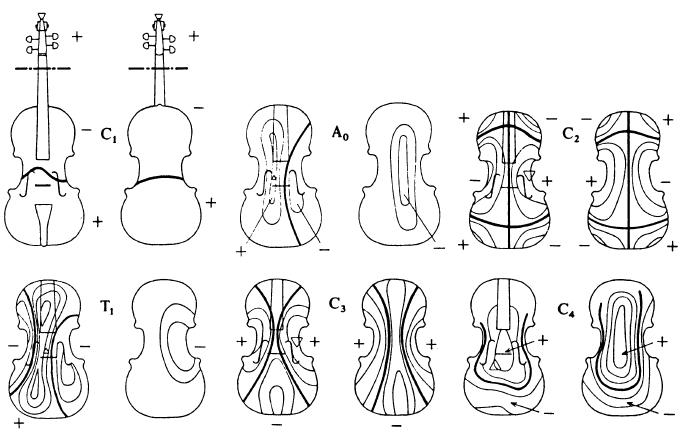
\includegraphics[width=0.7\linewidth]{00_Images/03_chapter/img189.jpg}
\caption{Representative violin body modes at low frequency}
\label{fig:violin_signature_modes}
\end{figure}

\paragraph{Component analysis in lutherie} In practical making and setup, it is useful to analyze the vibrational modes of different components separately, to obtain hints on the assembled outcome. Air modes can be estimated by building rigid-wall cavities with violin-like shape, by immersing the instrument in sand, or by finite element analysis, with results that are generally in good agreement. A schematic view related to cavity (air) modes and their identification is shown in figure \ref{fig:violin_air_modes}.

\begin{figure}[!htb]
\centering
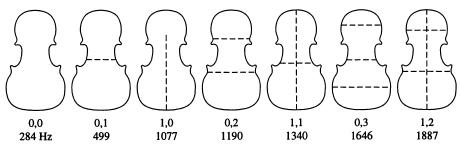
\includegraphics[width=0.7\linewidth]{00_Images/03_chapter/img206.jpg}
\caption{Illustration related to violin cavity (air) modes}
\label{fig:violin_air_modes}
\end{figure}

\paragraph{Free plates and assembled body} The modal frequencies of free plates are not directly related to those of the assembled body, because complex coupling arises when plates are mounted together with back and ribs. Tuning selected free-plate modes, such as the X-mode (mode \#2) and the ring mode (mode \#5), approximately one octave apart in the two plates are proposed by some studies. Given the X-mode frequencies, it has been suggested that the intended use of the instrument can be anticipated. For cellos, mode \#1 can be tuned about one octave below mode \#2 in both plates, while in violins the corresponding interval should be less than an octave in the back plate. Examples of free-plate mode shapes (often visualized via Chladni patterns) are shown in figure \ref{fig:free_plate_modes_chladni}.

\begin{figure}[!htb]
\centering
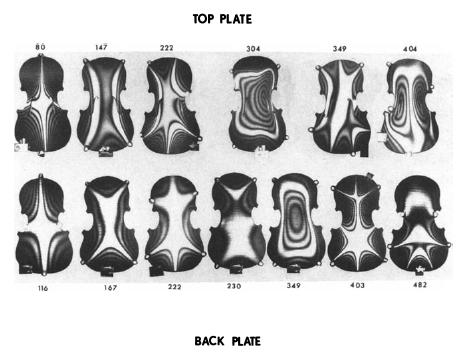
\includegraphics[width=0.7\linewidth]{00_Images/03_chapter/img220.jpg}
\caption{Free-plate mode shapes for top and back plates}
\label{fig:free_plate_modes_chladni}
\end{figure}

\section{Transient Wave Response of the Violin Body}

\subsection{Impulse Excitation at the Bridge}

Besides steady-state admittance and modal shapes, it is important to study the short-time response of the violin body to impulsive forces applied at the bridge. In particular, both transversal and longitudinal impulsive excitations are relevant, because they correspond to different directions of the string-bridge interaction and they trigger different wave-like motions in the plates. Transient wave propagation following impulsive excitation is illustrated by interferograms in figure \ref{fig:violin_transient_interferograms}.

\begin{figure}[!htb]
\centering
\subfloat{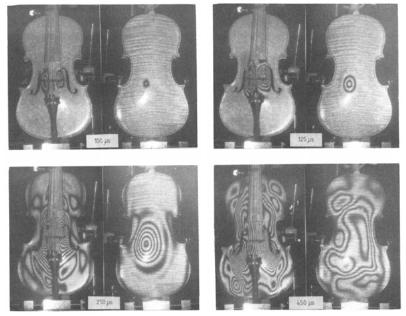
\includegraphics[height=0.3\textheight]{00_Images/03_chapter/img236.jpg}}\hfill
\subfloat{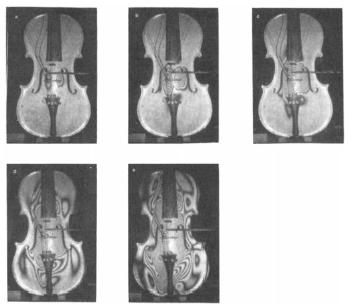
\includegraphics[height=0.3\textheight]{00_Images/03_chapter/img250.jpg}}
\caption{Interferograms after impulsive excitation in two directions}
\label{fig:violin_transient_interferograms}
\end{figure}

\subsection{Impulse Parallel to the Top Plate}

When an impulsive force is applied parallel to the top plate at the bridge, interferograms of top and back plates show the development of transient deformation patterns on microsecond time scales. Representative snapshots reported at \( t = \SI{100}{\micro\second} \), \( \SI{125}{\micro\second} \), \( \SI{250}{\micro\second} \), and \( \SI{450}{\micro\second} \) highlight how the disturbance propagates away from the bridge region and excites coupled motion of both plates. 

\subsection{Impulse Orthogonal to the Top Plate}

If the impulsive force is orthogonal to the top plate, the transient response differs markedly. Interferograms at \( t = \SI{70}{\micro\second} \), \( \SI{120}{\micro\second} \), \( \SI{150}{\micro\second} \), \( \SI{230}{\micro\second} \), and \( \SI{300}{\micro\second} \) show patterns that are distinct from the parallel-force case, indicating that the initial loading direction selects different families of plate motion and coupling mechanisms. 

\subsection{Phase Relation Between Bridge Feet}

A key qualitative difference between the two excitations concerns the phase relation of the impulses transmitted through the bridge feet.

\begin{itemize}
    \item For a force parallel to the plate, the pulses transmitted to the treble and bass feet are equal in magnitude but opposite in phase.
    \item For a transversal input, the original pulses have the same phase on the two sides of the bridge.
\end{itemize}

This difference explains why the observed interferometric patterns for the two loading directions are not simply scaled versions of each other, but instead exhibit different spatial organizations from the earliest instants after the impulse. 

\section{Soundpost and Bass Bar}

The vibroacoustic behavior of the violin body is rendered asymmetrical by the presence of the soundpost and the bass bar, located approximately beneath the treble and bass feet of the bridge, respectively. Strings are excited mainly parallel to the top plate, thus inducing a rocking motion of the bridge. Below the first resonance of the bridge, typically around \SI{2500}{\hertz} for a violin, the forces exerted on the two bridge feet are approximately equal in magnitude and opposite in phase. In a perfectly symmetric instrument, such a loading would preferentially excite only antisymmetric body modes, while strongly radiating symmetric modes would be driven only weakly. In practice, the asymmetry introduced by soundpost and bass bar alters this selection mechanism and contributes to the excitation of efficiently radiating motions. 

\subsection{Role of the Bass Bar}

The main function of the bass bar is to stiffen the top plate, both statically and dynamically. In many valuable historical instruments the bass bar has been modified over time, because modern strings exert higher tension than in the past and a stiffer support of the top plate becomes necessary.

\subsection{Role of the Soundpost} 

The soundpost mechanically couples the top and back plates. To clarify its effect, several investigators have compared violins with and without a soundpost. One reported set of observations found that removing the soundpost produced the following changes: 

\begin{itemize}
    \item It lowered the frequencies of the \( A0 \) and \( T1[B1] \) modes by \( 8\% \) and \( 13\% \), respectively.
    \item It made the \( T1 \) mode comparatively more symmetric.
    \item It raised the frequency of the \( C3 \) mode by about \( 2\% \).
    \item It left the \( A1 \) internal air mode essentially unchanged.
    \item It introduced a \( T2 \) mode, consisting largely of antisymmetric bending of the top plate.
\end{itemize}

As a consequence, in the presence of the soundpost, the strongly radiating \( T1 \) mode can be interpreted as a combination of a symmetric \( T1 \)-type motion and an antisymmetric \( T2 \)-type contribution. Another study suggests that removing the soundpost may leave the frequencies of \( T1 \) and \( C3 \) virtually unchanged while significantly modifying the corresponding mode shapes, with a dramatic decrease in radiation efficiency (estimated from measured mode shapes via boundary element methods) in the \SIrange{500}{800}{\hertz} range. These results are consistent with practical experience: violin makers and performers observe that moving the soundpost by a small distance can cause marked changes in the perceived sound of the instrument. 

\section{The Bridge}

The bridge transforms the motion of the vibrating strings into periodic driving forces applied to its feet and then to the top plate. Because it sits at the main mechanical interface between strings and body, any modification to the bridge can alter the instrument response and, consequently, the perceived sound. A convenient frequency-domain description uses the input impedance at the string notch and the force transfer from the notch to the two feet. If \( F_{\mathrm{in}}(\omega) \) and \( V_{\mathrm{in}}(\omega) \) are the force and velocity at the notch, and \( F_i(\omega) \) is the force delivered to foot \( i \), one may write
\[
Z_{\mathrm{in}}(\omega) = \frac{F_{\mathrm{in}}(\omega)}{V_{\mathrm{in}}(\omega)}, \quad H_i(\omega) = \frac{F_i(\omega)}{F_{\mathrm{in}}(\omega)}
\]
Measured curves show that the transfer to the two feet is not identical: the foot on the soundpost side and the foot on the bass bar side can exhibit different resonant features, reflecting the asymmetry of the coupled bridge-body system. The bridge mechanical response, including input impedance and force transfer, is shown in figure \ref{fig:bridge_impedance_force_transfer}.

\begin{figure}[!htb]
\centering
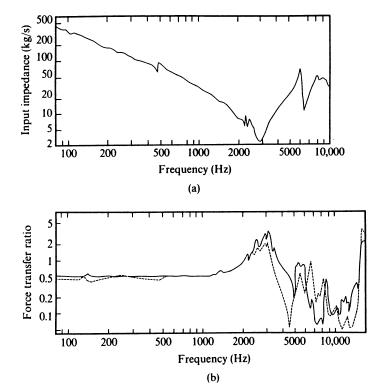
\includegraphics[width=0.7\linewidth]{00_Images/03_chapter/img267.jpg}
\caption{Bridge response: input impedance and force transfer ratio versus frequency}
\label{fig:bridge_impedance_force_transfer}
\end{figure}

\paragraph{First bridge resonances and mode shapes} The first two vibrational modes of a violin bridge occur in the kilohertz range and have distinct deformation patterns. The first resonance is mainly a rotation of the upper part of the bridge, while the second mode is efficiently excited by a vertical force. A comparison with a cello bridge highlights a different behavior: in the cello, the first modes are more strongly related to bending of the legs. This is attributed to the different bridge shape, characterized by more slender legs than the violin bridge. The first bridge modes and a comparison between violin and cello bridges are shown in figure \ref{fig:bridge_modes_violin_cello}.

\begin{figure}[!htb]
\centering
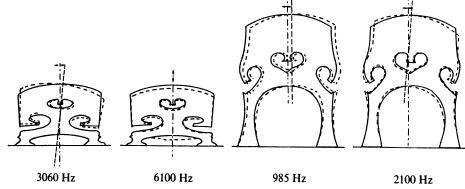
\includegraphics[width=0.7\linewidth]{00_Images/03_chapter/img281.jpg}
\caption{First bridge modes: comparison between violin and cello bridges}
\label{fig:bridge_modes_violin_cello}
\end{figure}

\paragraph{Practical modifications: added mass and added stiffness} Sometimes players modify the bridge response using simple interventions:

\begin{itemize}
    \item A mute, which acts mainly as a small added mass, tends to darken the sound by shifting bridge resonances toward lower frequencies.
    \item Small wedges pushed into bridge slits increase local stiffness and tend to raise modal frequencies.
\end{itemize}

A reported comparison of force transfer functions shows how an additional mass of about \SI{1.5}{\gram} and additional stiffness produce distinct shifts of the bridge resonances, confirming that relatively small changes at the bridge can have audible consequences. The effect of adding mass or stiffness to the bridge on force transfer is shown in figure \ref{fig:bridge_modifications_effect}.

\begin{figure}[!htb]
\centering
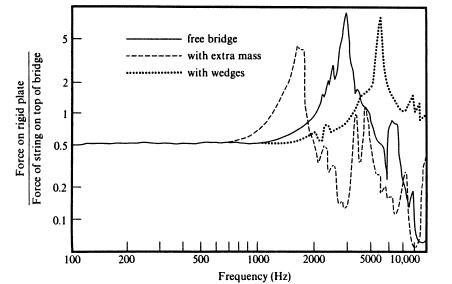
\includegraphics[width=0.7\linewidth]{00_Images/03_chapter/img295.jpg}
\caption{Effect of added mass and stiffness on bridge force transfer}
\label{fig:bridge_modifications_effect}
\end{figure}

\section{Coupling Between Bridge and Soundboard}

\subsection{Filtering Effect and Simplified Translation Model}

The coupling between bridge and soundboard can be described in terms of the input admittance seen by the strings at the bridge. Even a very simple coupled model already highlights an important consequence: the bridge does not transmit string forces uniformly with frequency, but introduces a filtering effect that shapes the response. A schematic model for the coupling between bridge motion and soundboard dynamics is shown in figure \ref{fig:bridge_soundboard_coupling_model}. A first approximation models the bridge as a lumped mass-spring system \( (m,k) \) loaded by the board admittance \( Y(\omega) \) at the attachment point. Denoting by \( V_b \) the bridge velocity at the string junction and by \( V_t \) the velocity of the board translation, the equations of motion are
\[
\begin{aligned}
&-m\omega^{2}V_b + k(V_b - V_t) = j\omega F \\
&V_t = Y(\omega)F_t = \frac{kY(\omega)}{j\omega}(V_b - V_t)
\end{aligned}
\]
The input admittance at the bridge is defined as
\[
Y_b(\omega) = \frac{V_b}{F}
\]
and it can be written as
\[
Y_b(\omega) = \frac{kY(\omega)+j\omega}{k-m\omega^{2}+j\omega k m Y(\omega)}
\]
If the bridge base is fixed, \( Y(\omega) = 0 \), the system reduces to a series resonance corresponding to the bridge eigenmode. In all other cases, the input admittance depends on the board mobility \( Y(\omega) \) and the resulting modulus \( |Y_b| \) can exhibit a pronounced peak in the kilohertz range, consistent with the bridge-hill feature observed in violin measurements.

\begin{figure}[!htb]
\centering
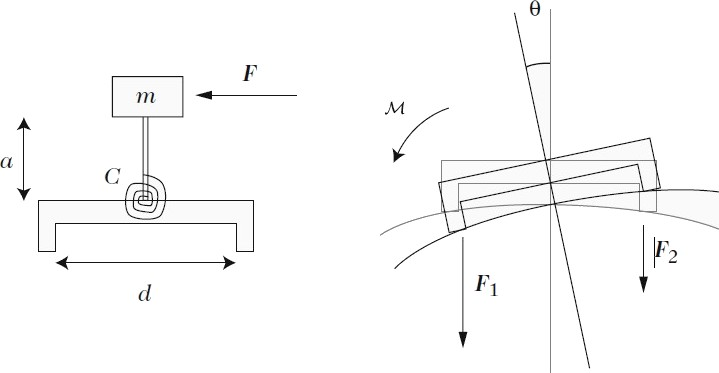
\includegraphics[width=0.7\linewidth]{00_Images/03_chapter/img385.jpg}
\caption{Model of coupling between bridge and soundboard}
\label{fig:bridge_soundboard_coupling_model}
\end{figure}

\subsection{Refined Model Including Bridge Rotation}

The previous model captures the existence of a bridge-related filtering peak, but it does not include any bridge geometry. A more realistic description accounts for the bridge rotation driven by the horizontal string force. Let the string apply a horizontal force \( F \) at a mean lever arm \( a \), generating a moment
\[
M = Fa
\]
The bridge rotation \( \theta \) is described by a torsional stiffness \( C \) and an effective rotational inertia \( ma^{2} \), so that
\[
M = ma^{2}\ddot{\theta}+C\theta
\]
and the corresponding angular eigenfrequency is
\[
\omega_b = \sqrt{\frac{C}{ma^{2}}}
\]
The bridge is connected to the soundboard through two feet separated by a distance \( d \). Under the forces \( (F_1,F_2) \), the foot velocities \( (V_1,V_2) \) satisfy an admittance-matrix relation
\[
\begin{bmatrix}
V_1 \\
V_2
\end{bmatrix}
 = 
\begin{bmatrix}
Y_{11} & Y_{12} \\
Y_{21} & Y_{22}
\end{bmatrix}
\begin{bmatrix}
F_1 \\
F_2
\end{bmatrix}
\]
With one foot fixed, a moment \( M \) can be represented by the equivalent force couple
\[
F_1 = \frac{M}{d^{2}}, \quad F_2 = -\frac{M}{d^{2}}
\]
leading to
\[
\begin{bmatrix}
\dot{\theta}_1 \\
\dot{\theta}_2
\end{bmatrix}
 = 
\begin{bmatrix}
Y_{11} & Y_{12} \\
Y_{21} & Y_{22}
\end{bmatrix}
\begin{bmatrix}
\dfrac{M}{d^{2}} \\
-\dfrac{M}{d^{2}}
\end{bmatrix}
\]
The bridge rotational velocity is \( \dot{\theta} = \dot{\theta}_1-\dot{\theta}_2 \), hence the rotational admittance is
\[
Y_r(\omega) = \frac{\dot{\theta}}{M} = \frac{Y_{11}+Y_{22}-2Y_{12}}{d^{2}}
\]

\subsection{Rotational Admittance in Modal Form and Bridge Input Admittance}

The rotational admittance can be expressed in modal form in terms of soundboard eigenshapes \( \phi_n \), evaluated at the two foot locations \( (x_1,y_1) \) and \( (x_2,y_2) \),
\[
Y_r(\omega) = j\omega\frac{1}{d^{2}}
\sum_{n}
\frac{\left[\phi_n(x_1,y_1)-\phi_n(x_2,y_2)\right]^{2}}
{m_n\left(\omega_n^{2}+2j\omega\omega_n\zeta_n-\omega^{2}\right)}
\]
where \( m_n \) is the modal mass, \( \omega_n \) the eigenfrequency, and \( \zeta_n \) the modal damping ratio. Finally, the bridge input admittance follows by noting that the bridge velocity at the string notch is \( V_b = a\dot{\theta} \) and \( M = Fa \), so
\[
Y_b(\omega) = \frac{V_b}{F} = a^{2}\frac{\dot{\theta}}{M}
\]
and substituting the bridge rotational dynamics yields
\[
Y_b(\omega) = 
\frac{a^{2}\left[CY_r(\omega)+j\omega\right]}
{C-ma^{2}\omega^{2}+j\omega Cma^{2}Y_r(\omega)}
\]
This refined model is more accurate than the translational one and explicitly shows how manufacturing parameters, such as the bridge height \( a \) and the foot spacing \( d \), influence the filtering action of the bridge-soundboard coupling.

\section{Sound Radiation}

\subsection{Radiated Sound Pressure Level and Spectral Decay}

Sound radiation can be characterized by measuring the sound pressure level (SPL) at a set of microphones placed around the instrument and averaging the results. For a violin driven by a sinusoidal excitation at the bridge and measured at \SI{1}{\meter}, the averaged radiated spectrum shows a clear decay above about \SI{700}{\hertz}. In particular, the total radiated power decreases at approximately \SI{9}{\decibel} per octave. If the excitation is instead provided by normal bowing, a steeper overall decrease is expected, around \SI{15}{\decibel} per octave. This can be interpreted as the combination of the bow-excitation spectral decay (about \SI{6}{\decibel} per octave) and the \SI{9}{\decibel} per octave trend associated with the instrument radiation. A representative radiated sound pressure level spectrum is shown in figure \ref{fig:violin_spl_spectrum}.

\begin{figure}[!htb]
\centering
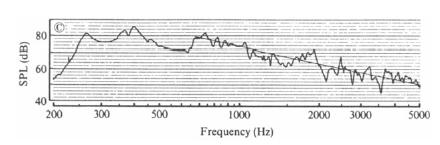
\includegraphics[width=0.9\linewidth]{00_Images/03_chapter/img402.jpg}
\caption{Radiated sound pressure level versus frequency}
\label{fig:violin_spl_spectrum}
\end{figure}

\subsection{Directivity and Frequency Dependence}

A directional analysis of the radiated sound highlights a change of behavior above a characteristic frequency on the order of \SI{1000}{\hertz}. 

\begin{itemize}
    \item Below that frequency, the radiation pattern is smooth and the instrument is approximately omnidirectional, especially below \SI{500}{\hertz}.
    \item Above about \SI{1000}{\hertz}, the instrument becomes progressively more directive.
    \item Near a resonance, small changes in frequency can produce dramatic changes in the radiation pattern.
\end{itemize}

\subsection{Directional Characteristics at Selected Frequencies}

Polar radiation plots measured on different violins driven sinusoidally at the bridge illustrate how the directivity evolves across frequency. Representative patterns reported at frequencies such as \SI{695}{\hertz}, \SI{875}{\hertz}, \SI{625}{\hertz}, and \SI{650}{\hertz} show that even in a relatively narrow band, the radiated field can differ substantially between instruments and between nearby frequencies. Directional characteristics of violin radiation at a representative frequency are shown in figure \ref{fig:violin_directivity_comparison}.

\begin{figure}[!htb]
\centering
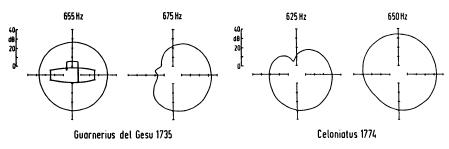
\includegraphics[width=0.8\linewidth]{00_Images/03_chapter/img418.jpg}
\caption{Directional characteristics of radiated sound for two violins}
\label{fig:violin_directivity_comparison}
\end{figure}

\subsection{Principal Radiation Directions}

If directivity characteristics are averaged over wider frequency ranges and over multiple instruments, one obtains a set of principal radiation directions. These can be summarized by showing the angular regions within \SI{3}{\decibel} of the maximum on selected planes, for instance on horizontal and vertical planes for the cello, and on the horizontal plane for the violin. A compact summary of the main radiation directions (in terms of \SI{3}{\decibel} regions) is shown in figure \ref{fig:violin_radiation_3db_regions}.

\begin{figure}[!htb]
\centering
\subfloat{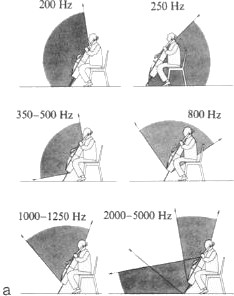
\includegraphics[width=0.3\linewidth]{00_Images/03_chapter/img442_1.jpg}}\hfill
\subfloat{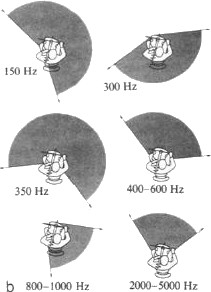
\includegraphics[width=0.3\linewidth]{00_Images/03_chapter/img442_2.jpg}}\hfill
\subfloat{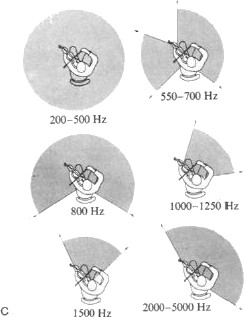
\includegraphics[width=0.3\linewidth]{00_Images/03_chapter/img442_3.jpg}}
\caption{Main radiation directions summarized as \SI{3}{\decibel} regions}
\label{fig:violin_radiation_3db_regions}
\end{figure}
 
\section{The Wolf Notes}

A wolf note is an unstable regime that arises from a strong coupling between the bowed string and a prominent body resonance. An example illustrating the temporal behavior during a wolf note is shown in figure \ref{fig:wolf_note_oscillograms}.

\begin{figure}[!htb]
\centering
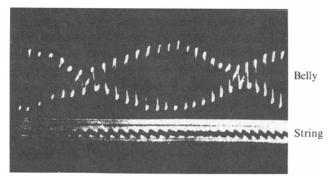
\includegraphics[width=0.7\linewidth]{00_Images/03_chapter/img457.jpg}
\caption{Example oscillograms during a wolf note}
\label{fig:wolf_note_oscillograms}
\end{figure}

\paragraph{Impedance mismatch and cyclic energy transfer} In normal conditions, the characteristic impedance of a string is about \( 1/10 \) of the bridge impedance as seen by the string. This mismatch is usually large enough to treat the bridge as effectively rigid, providing the strong reflection needed for oscillations to build up on the string. At the frequency of a strong body resonance, however, the bridge impedance is greatly reduced. The resulting reflection can become too weak to compensate the losses inherent to the string motion. The interaction can then proceed as follows:

\begin{itemize}
    \item Initially, the bridge still provides a sufficiently strong reflection for the string oscillation to build up.
    \item As the body vibration builds up near the resonance, the bridge appears comparatively soft to the string and absorbs energy, causing the string oscillation to die down.
    \item When the string oscillation weakens, the body vibration is deprived of its energy source and decays as well, enabling the cycle to start again.
\end{itemize}

\paragraph{Amplitude exchange and perceived roughness} The net result is an alternation in which string and body vibrations grow and diminish in amplitude in turn. The perceived tone varies strongly and harshly at an exchange frequency that is typically about \SI{5}{\hertz}.

\paragraph{Why cello and viola are more prone} The instruments most prone to wolf notes are the cello and the viola. Their dimensions are not scaled proportionally to the wavelength of the sounds they produce, so the impedance mismatch between bridge and string is reduced with respect to the violin. In addition, the larger bridge height acts as a longer lever, further reducing the impedance seen by the string. The wolf note is most likely to be triggered under light bowing, because the exerted force may be insufficient to compensate the losses.

\paragraph{Simulation evidence} A simple simulation can reproduce the phenomenon by adding a single body resonance at the same frequency as the fundamental of the string. The time histories show a visible modulation of the string velocity, associated with an alternation between Helmholtz motion and a double-slipping regime. In the simulated behavior, Helmholtz motion breaks down when body motion reaches a high value and resumes when body motion becomes sufficiently small.

\section{Electric Analog of the Violin}

The violin can be interpreted as a broadband radiator obtained by distributing many relatively narrow resonances across frequency, rather than by relying on one or two nearly aperiodic bands. In the upper octaves the wooden body provides a sufficiently dense set of resonances to yield a quasi-uniform response, while in the lower octaves the series ends and a prominent resonance in the vicinity of \SI{460}{\hertz} is often identified as the main body resonance. Without additional reinforcement below this region, the response would tend to decrease rapidly with frequency. The air resonance associated with the cavity breathing through the f-holes supports the response over part of the next octave. A further point is that subjective uniformity is not solely determined by the objective frequency response. A strengthened harmonic can increase the perceived strength of the corresponding fundamental, reducing the perceptual impact of dips in the measured curve and contributing to tone-color differences. An overview of an electrical analog representation of the violin is shown in figure \ref{fig:violin_electric_analog_overview}. 

\begin{figure}[!htb]
\centering
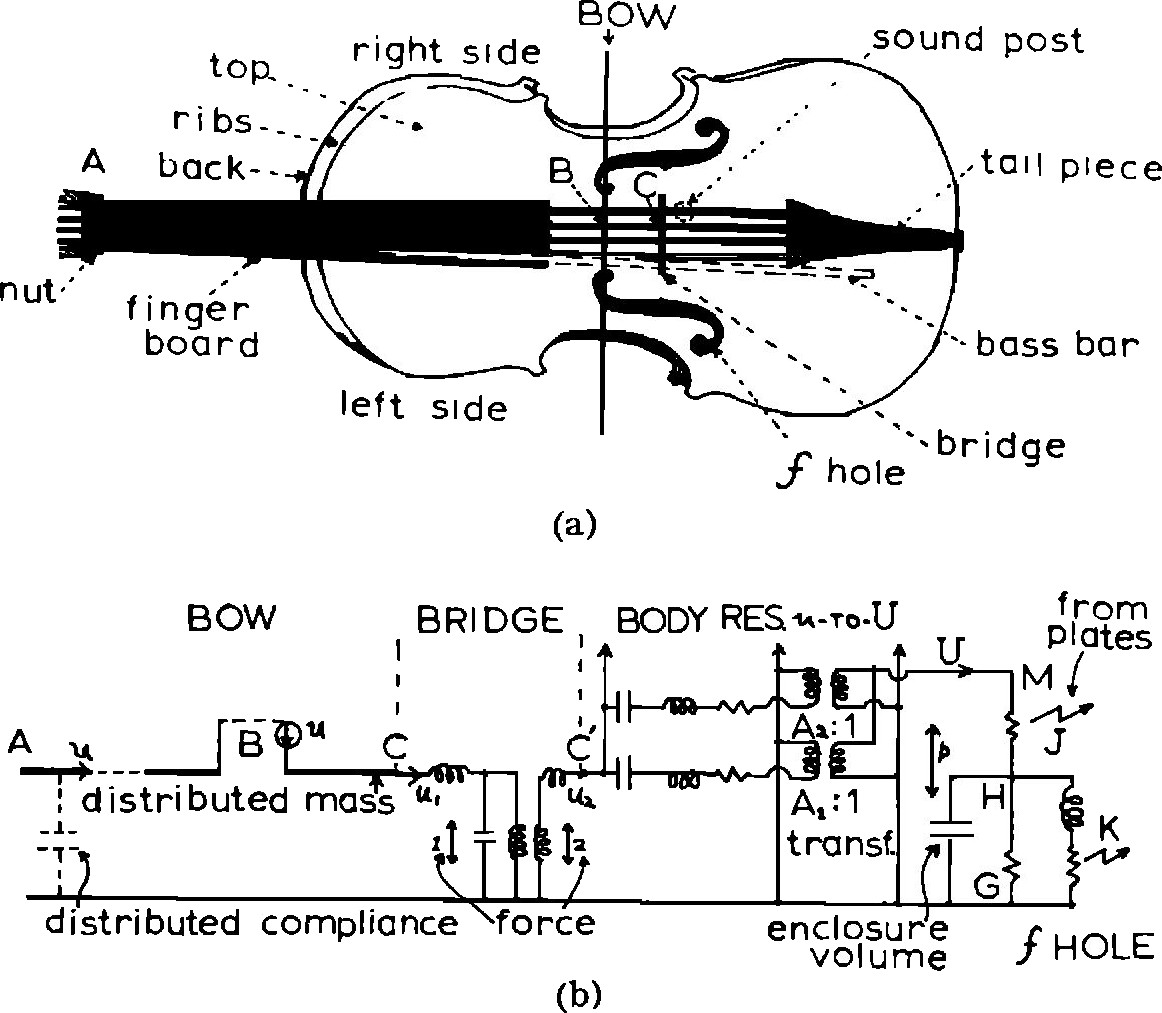
\includegraphics[width=0.7\linewidth]{00_Images/03_chapter/img476.jpg}
\caption{Overview of an electrical analog of the violin}
\label{fig:violin_electric_analog_overview}
\end{figure}

\subsection{String}

In an electrical analogy based on the impedance (force-velocity) convention, the circuit begins at the bow-string contact, which can be represented by a negative resistance. Under the Helmholtz model of bowed-string motion, the bow-string contact behaves as a velocity generator, and the contact point is in series with the two string segments it defines. The two segments have different reactive characters: the segment toward one end can be treated as a positive mechanical reactance, while the other appears as a negative reactance, except as modified by the bridge. Taken together, the two parts form a distributed resonant system. Since the traveling-wave wavelength on the string is comparable with the string length, a transmission-line representation is appropriate.

\subsection{The Bridge}

The bridge is the transducer that accepts power from the string and conveys it to the body, which then excites both the surrounding air and the internal cavity air. Since bridge resonances occur at frequencies high with respect to the lower octaves of the string, the bridge can be regarded as effectively rigid in that range and modeled mainly as a transformer, without introducing a dominant filtering effect there. 

\subsection{The Soundpost}

At low frequencies, the soundpost can be approximated as an element that connects top and back plates together with the ribs. In addition, the soundpost is a main source of asymmetry in mode shapes, which contributes to more efficient radiation than would be expected for a perfectly symmetric structure excited in a purely antisymmetric manner.

\subsection{The Body Modes}

The f-holes, even if narrowed through historical evolution, remain relevant in sound emission, especially for the breathing-type air motion. In the impedance view, the body response exhibits alternating resonances and antiresonances. Due to losses and radiation, resonant impedances do not reach zero. A key observation is that body resonances do not necessarily correspond to maxima in the acoustic response, because many structural modes radiate poorly. Modes with efficient radiation properties play a disproportionate role in the radiated output. In the circuit representation, plate modes can be rendered as a parallel set of resonant branches connected at the bridge coupling point. 

\subsection{The Air Mode}

Air modes represent efficient radiators and form a notable exception to the previous observation. In the circuit, this contribution is described in terms of volume velocity and coupled through a mechanical-to-acoustical transformer with ratio \( A:1 \), where \( A \) depends on the mode considered. The radiation through the f-holes is represented by the branch associated with the apertures. Since the apertures are not circular and the violin walls are not rigid, the resonance frequency is not expected to coincide exactly with the ideal Helmholtz value. Nevertheless, experiments indicate that the deviation remains limited even with non-rigid walls, and it stays small for approximately elliptical apertures with modest eccentricity. 

\subsection{Simplified Circuit: Air Resonance and One Body Resonance}

If only the air resonance and the main body resonance are retained, a simplified network is obtained in which one resonant body branch is combined with the air branch, and the coupling is referred to the bridge. This reduced description is useful to interpret how the lower register can be strengthened by matching the air resonance and the main body resonance, rather than treating them as isolated phenomena.

\subsection{Loss Mechanisms}

Within the simplified circuit, a transient associated with the air branch suffers from losses due to thermal and viscous effects in air, losses within the wood, and radiation losses. It is found that wood-related losses are typically much larger than those associated with air viscosity, so the dominant contributions are radiation and wood losses. As the air volume of the enclosure increases, radiation losses increase while wall-related losses decrease, leading to a trade-off that can be explored by varying geometric parameters. 

\subsection{Rib Height and Loss Balance}

By fixing top and back plates and varying rib height, the combined losses show a minimum at an intermediate rib height. The reported trend indicates that the rib height that minimizes the total losses is close to the rib height found in standard violin construction. 

    %! TEX rootmain.tex

\chapter{Reed and Lip Excitation}

In many wind instruments, sound is produced by the interaction between a quasi-steady air supply and a vibrating element that behaves as a valve. Reeds and lips can be treated as pressure-controlled valves, whose motion is driven by the pressure difference across the valve and whose vibration is shaped by the coupling with the instrument air column. The chapter first introduces a practical classification of these valves and a qualitative overview of the sound-generation mechanism. It then moves to reed modeling, discusses the role of nonlinearities in enabling self-oscillations, and interprets the reed as an acoustic generator coupled to a resonator. Finally, the large-amplitude regime is addressed, where the valve motion and the resulting flow modulation depart significantly from small-signal behavior.

\section{Valve Categories}

\subsection{Pressure-controlled Valves}

Several wind-instrument exciters can be regarded as pressure-controlled valves. Examples include single-reed systems such as the clarinet or saxophone, double reeds such as the oboe or bassoon, organ-reed pipes, and the player’s lips in brass instruments. In all cases, the valve motion is controlled by the pressure difference across the valve. The vibration frequency is controlled partly by the natural frequency of the reed and partly by the resonances of the instrument air column to which it is connected. A compact overview of common pressure-controlled valves is shown in figure \ref{fig:valve_categories_overview}.

\begin{figure}[!htb]
\centering
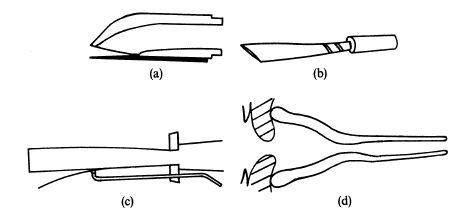
\includegraphics[width=0.7\linewidth]{00_Images/04_chapter/img28.jpg}
\caption{Examples of pressure-controlled valves used in wind instruments}
\label{fig:valve_categories_overview}
\end{figure}

\paragraph{Valve classification} A compact classification is obtained by introducing the doublet symbol \( (\sigma_1,\sigma_2) \), defined by the effect of steady pressure applied at the inlet and at the outlet:
\[
\begin{aligned}
\sigma_1 &= +1 && \text{if a pressure excess at the inlet tends to open the valve} \\
\sigma_1 &= -1 && \text{otherwise} \\
\sigma_2 &= +1 && \text{if a pressure excess at the outlet tends to open the valve} \\
\sigma_2 &= -1 && \text{otherwise}
\end{aligned}
\]
The classification can be visualized schematically as in figure \ref{fig:valve_classification_sigma}.

\begin{figure}[!htb]
\centering
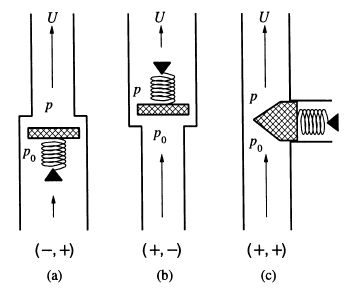
\includegraphics[width=0.7\linewidth]{00_Images/04_chapter/img63.jpg}
\caption{Valve classification based on the doublet \((\sigma_1,\sigma_2)\)}
\label{fig:valve_classification_sigma}
\end{figure}

\paragraph{Three valve types} Within this framework, three relevant valve types are distinguished:

\begin{itemize}
    \item \( (-,+) \): inward-striking valve, associated with woodwind reeds
    \item \( (+,-) \): outward-striking valve, associated with the player’s lips in one brass instrument model
    \item \( (+,+) \): sideways-striking valve, associated with the player’s lips in an alternative brass instrument model
\end{itemize}

The combination \( (-,-) \) is not useful in this context. The three relevant valve types are illustrated in figure \ref{fig:three_valve_types}.

\begin{figure}[!htb]
\centering
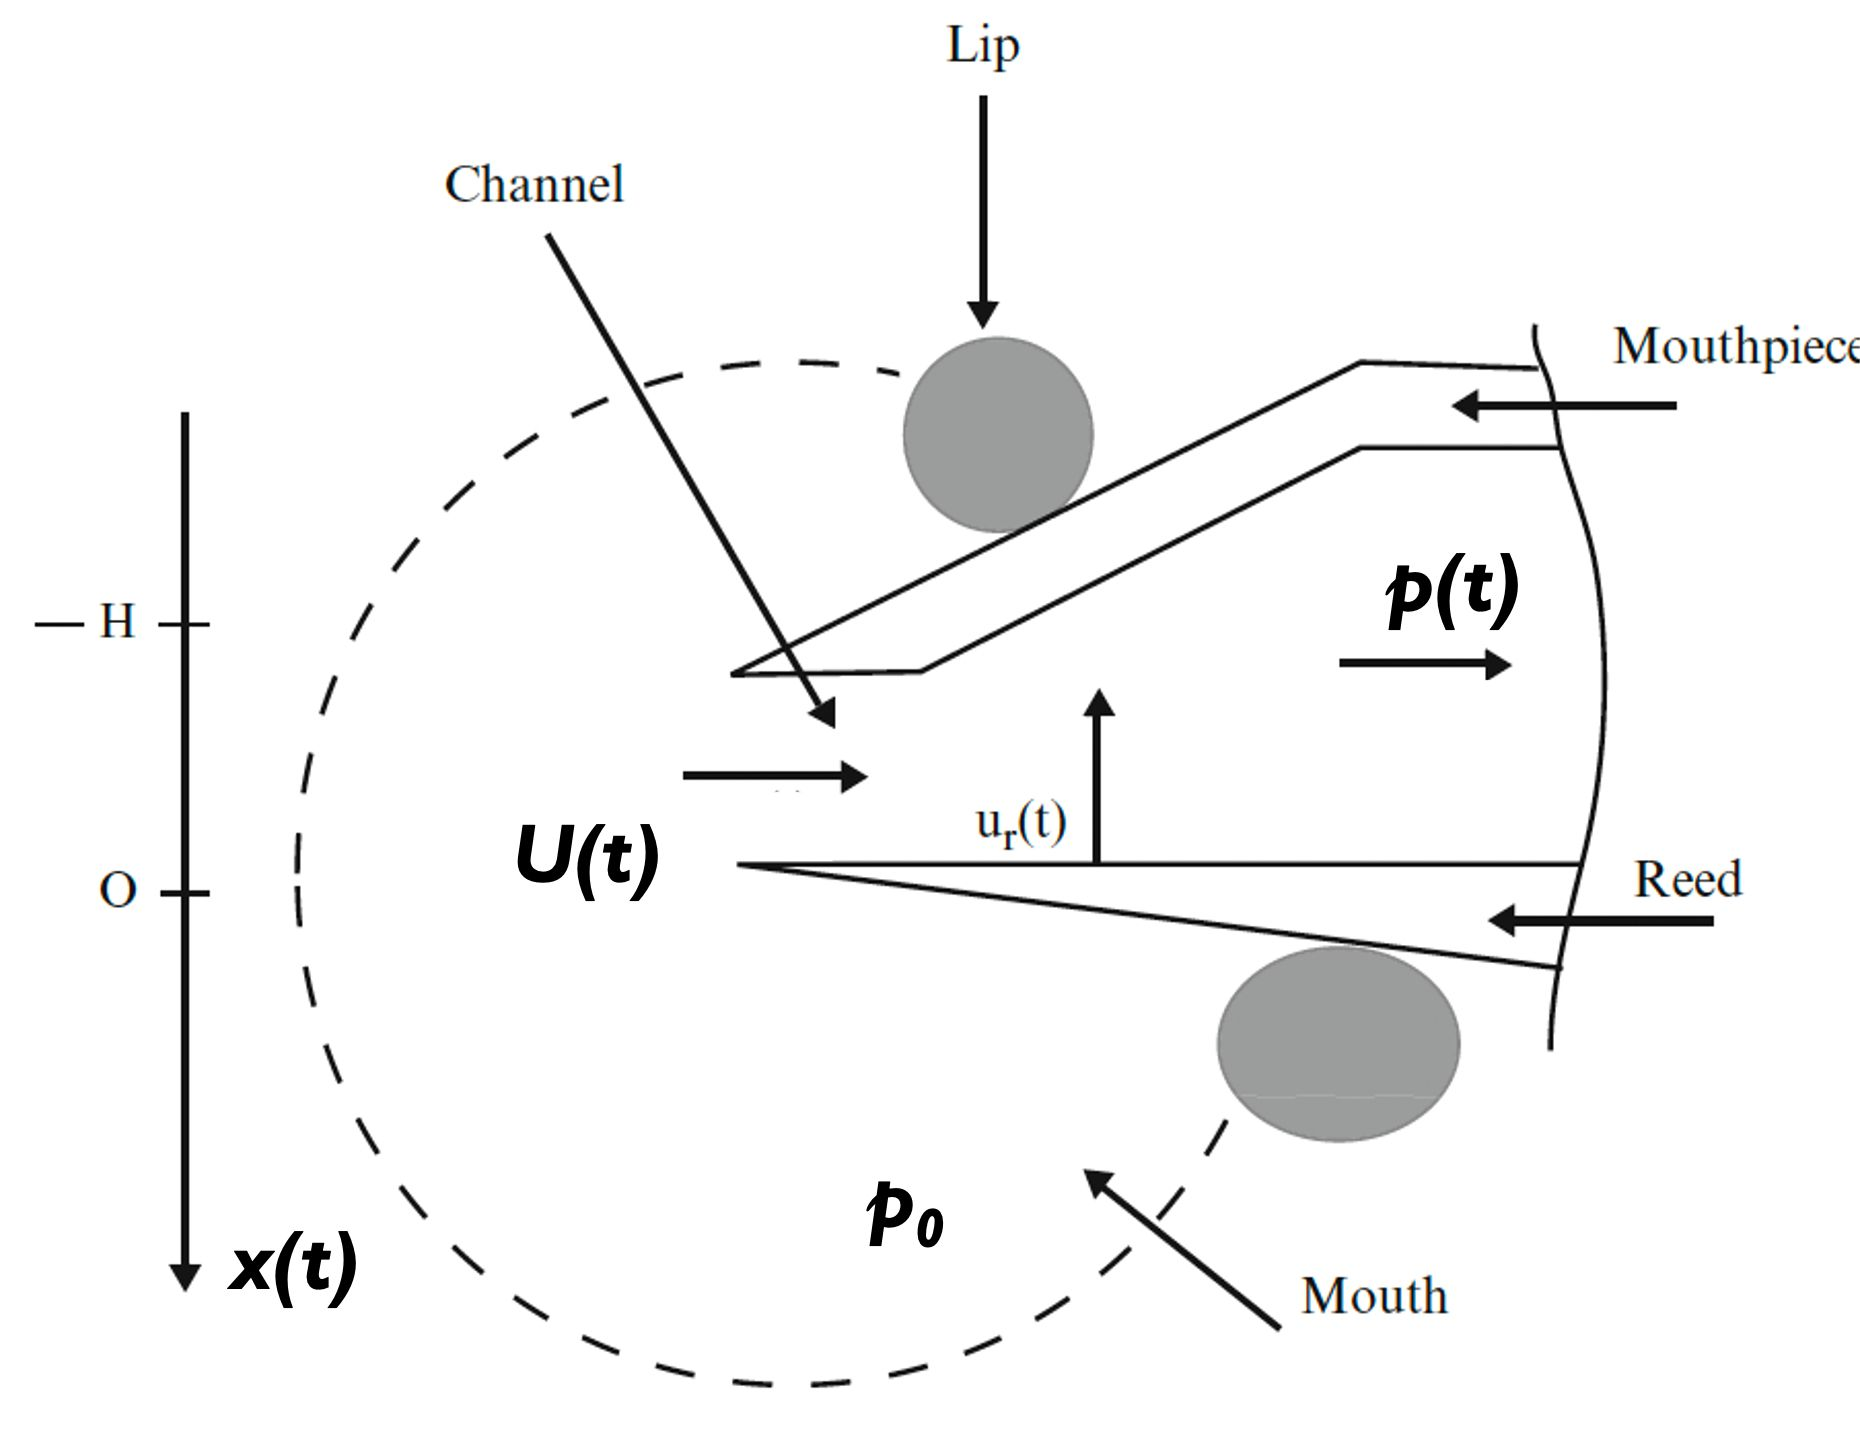
\includegraphics[width=0.7\linewidth]{00_Images/04_chapter/img73.jpg}
\caption{Inward-, outward-, and sideways-striking valve configurations}
\label{fig:three_valve_types}
\end{figure}

\subsection{Sound Generation in a Nutshell}

Blowing into the mouthpiece displaces the reed from its rest position. Because the reed is elastic, it tends to restore the displacement and can exhibit a complex oscillatory motion. This oscillation perturbs the air column in the reed channel and in the resonator. The resonance frequency is determined jointly by the elastic properties of the reed and the air column, indicating strong coupling between the mouthpiece and the resonator.

\subsection{Clarinet Reed}

The clarinet reed configuration is illustrated through lateral and top or bottom views, highlighting the reed geometry and its placement relative to the mouthpiece. Representative views of the clarinet reed geometry are given in figure \ref{fig:clarinet_reed_views}.

\begin{figure}[!htb]
\centering
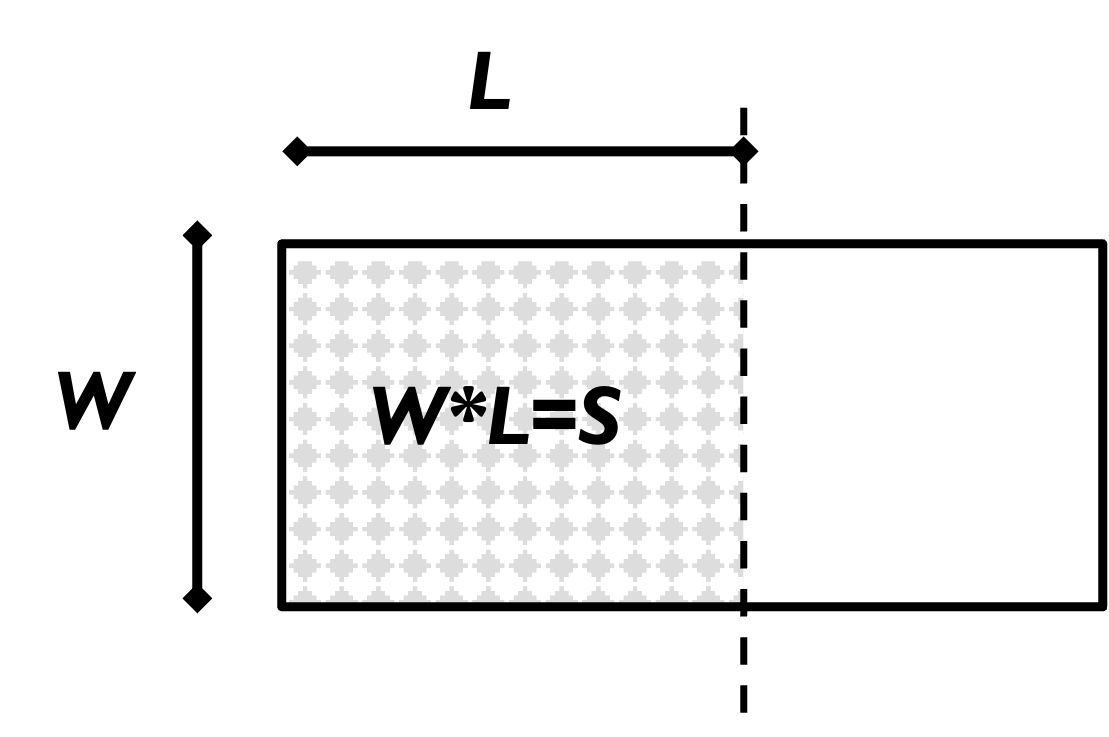
\includegraphics[width=0.6\linewidth]{00_Images/04_chapter/img75.jpg}
\caption{Clarinet reed geometry and placement relative to the mouthpiece}
\label{fig:clarinet_reed_views}
\end{figure}

\subsection{Lip Valves}

For lip valves, an excess of pressure at the inlet determines an opening of the valve, corresponding to \( \sigma_1 = +1 \). An excess of pressure at the outlet also determines an opening of the valve, corresponding to \( \sigma_2 = +1 \). A schematic representation of lip-valve operation is shown in figure \ref{fig:lip_valves_scheme}.

\begin{figure}[!htb]
\centering
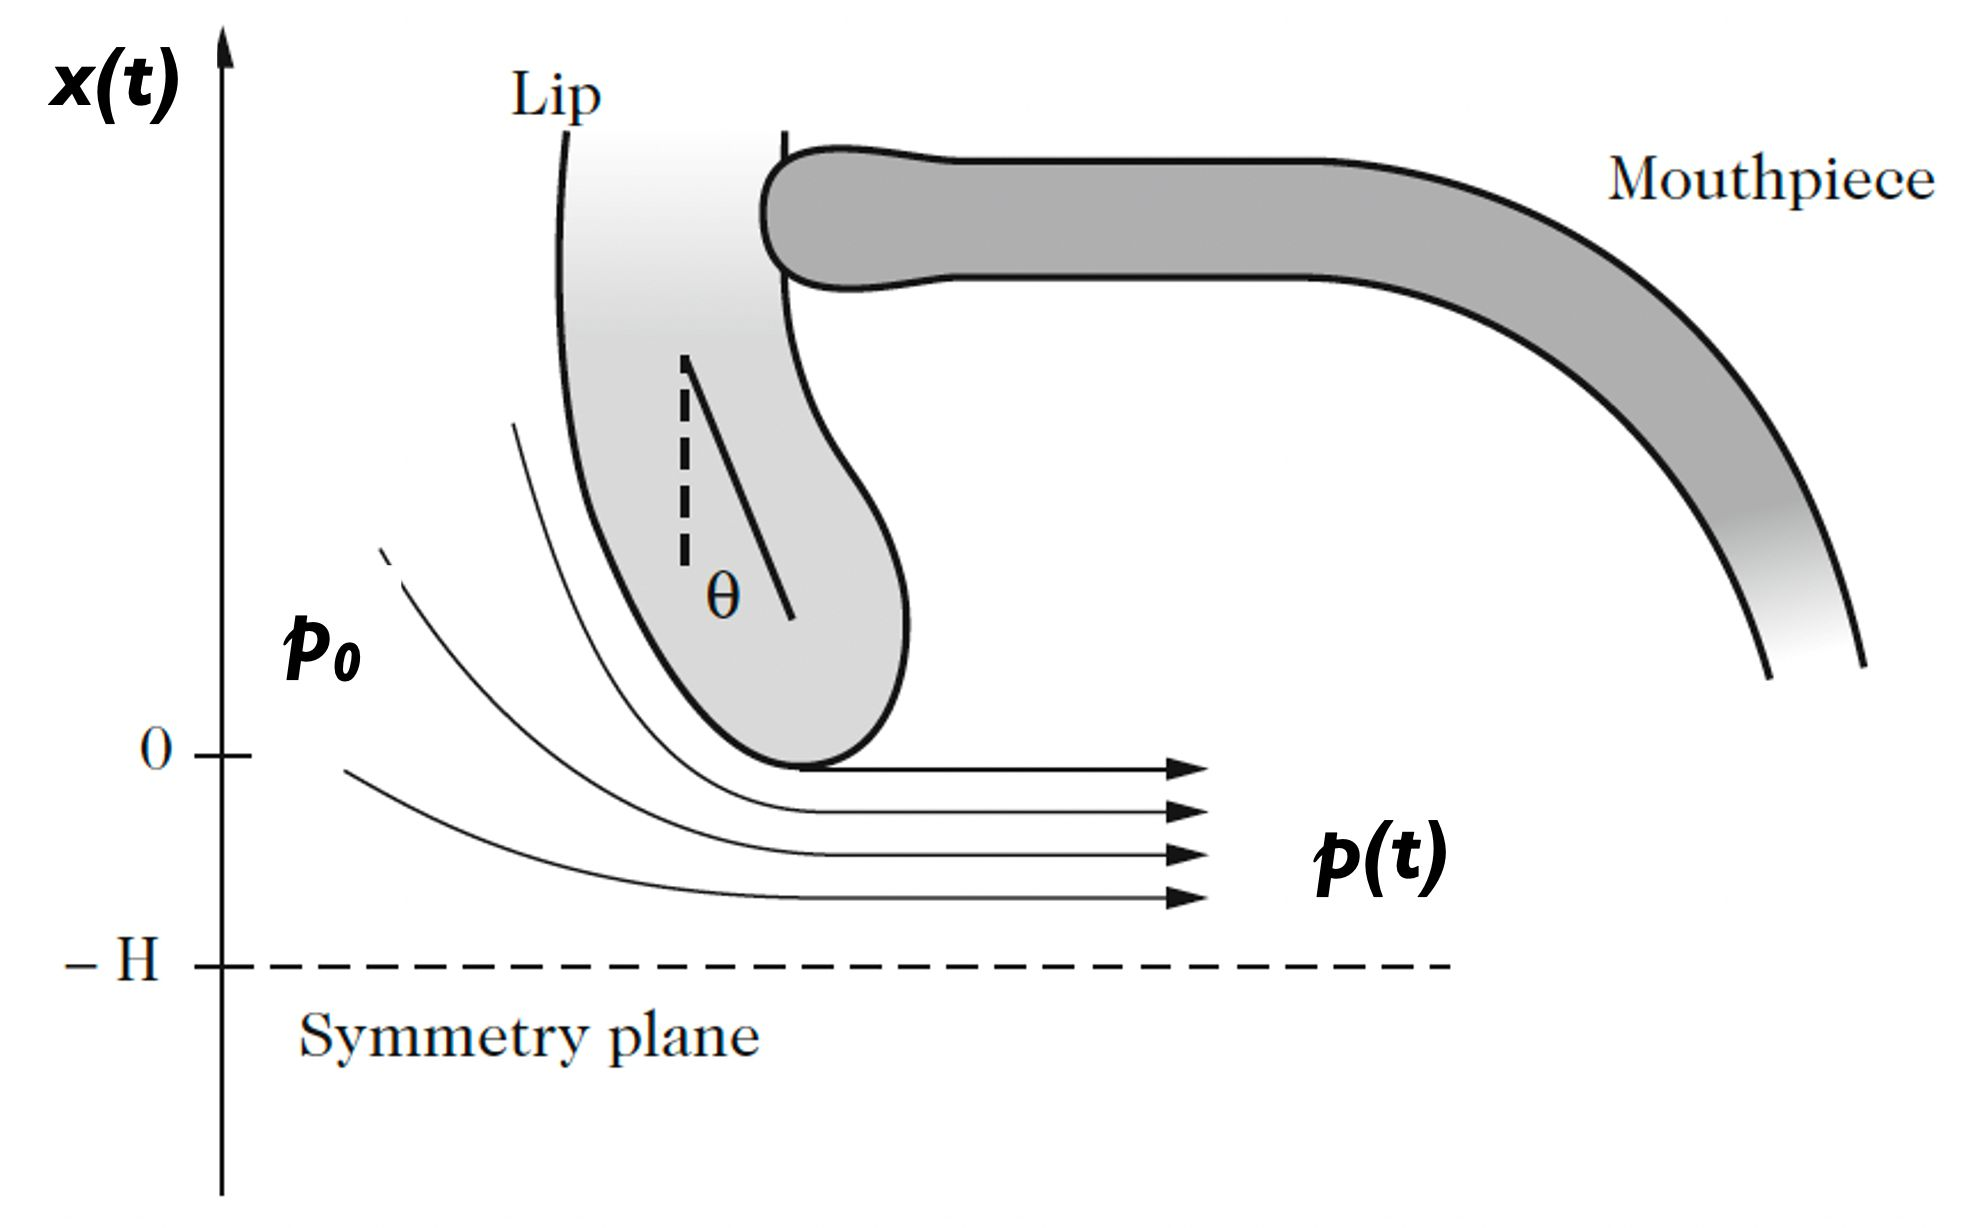
\includegraphics[width=0.6\linewidth]{00_Images/04_chapter/img82.jpg}
\caption{Lip valve as a pressure-controlled valve}
\label{fig:lip_valves_scheme}
\end{figure}

\section{Reed Quasi-static Modeling}

A first description of reed excitation can be built from a quasi-static flow model. Under the assumption of incompressible flow, Bernoulli’s principle relates flow speed and pressure along a streamline through
\[
\frac{v^2}{2} + gz + \frac{p}{\rho} = \text{const}
\]
where \( v \) is the flow speed, \( p \) the static pressure, \( \rho \) the fluid density, \( g \) the gravitational acceleration, and \( z \) the elevation. 

\paragraph{Flow through a valve} Consider a steady flow through a valve driven by an upstream pressure \( p_0 \) and an outlet pressure \( p \). Let \( x \) be the valve opening and \( W \) its width. After standard simplifications, the pressure drop \( p_0 - p \) can be related to the flow speed as
\[
p_0 - p = \frac{\rho v^2}{2}
\qquad
\Rightarrow
\qquad
v = \sqrt{\frac{2(p_0 - p)}{\rho}}
\]
so that the acoustic volume flow becomes
\[
U = Wxv = Wx\sqrt{\frac{2(p_0 - p)}{\rho}}
\]

\paragraph{Static reed opening} To close the model, the reed is represented as a spring with compliance \( C \). Denoting by \( x_0 \) the opening at rest and by \( S \) the effective reed area, the static deflection is written as
\[
x_0 - x = (\sigma_1 p_0 + \sigma_2 p)SC
\]
so that, after substitution into the expression for \( U \),
\[
U = W\left[x_0 - (\sigma_1 p_0 + \sigma_2 p)SC\right]\sqrt{\frac{2(p_0 - p)}{\rho}}
\]
This construction includes only a static force balance, and therefore defines a static reed model. 

\paragraph{Woodwind reed characteristic} For a woodwind reed, \( \sigma_1 = -1 \) and \( \sigma_2 = 1 \), which yields a characteristic of the form
\[
U = \sqrt{\alpha(p_0 - p)} - \sqrt{\beta(p_0 - p)^3}
\]
with constants \( \alpha \) and \( \beta \) collecting the geometric and mechanical parameters of the valve. The resulting \( (p_0 - p, U) \) characteristic is typically represented as a curve with distinct operating regions. A typical static characteristic for a woodwind reed, with the usual operating points, is shown in figure \ref{fig:woodwind_characteristic_OABC}.

\begin{figure}[!htb]
\centering
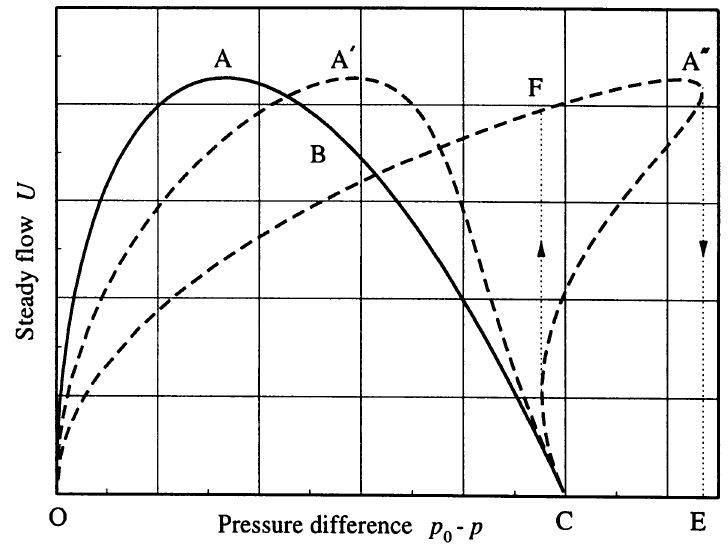
\includegraphics[width=0.7\linewidth]{00_Images/04_chapter/img99.jpg}
\caption{Woodwind reed quasi-static characteristic with operating regions}
\label{fig:woodwind_characteristic_OABC}
\end{figure}

\paragraph{Low-frequency admittance and negative resistance} The acoustic admittance presented by the reed to the instrument, at very low frequency, can be inferred from the characteristic curve through the slope
\[
G = \frac{\partial U}{\partial p}
\]
Where this slope is negative, the reed behaves as a negative resistance, namely as a flow generator. In the characteristic construction discussed in the slides, the negative-resistance region extends from A to C, with \( p_A = p_C/3 \), and a convenient operating point is B, for which \( p_B = 2p_C/3 \). 

\paragraph{Double reeds and additional flow resistance} In double-reed instruments such as oboe or bassoon, the narrow passage between the two reeds introduces an additional flow resistance \( R \). Changing \( R \) modifies the \( (p_0 - p, U) \) characteristic: the negative-resistance region can become narrower and steeper, and in some cases hysteresis may appear. The influence of an additional flow resistance on the static characteristic, including possible hysteresis, is illustrated in figure \ref{fig:double_reeds_resistance_effect}.

\begin{figure}[!htb]
\centering
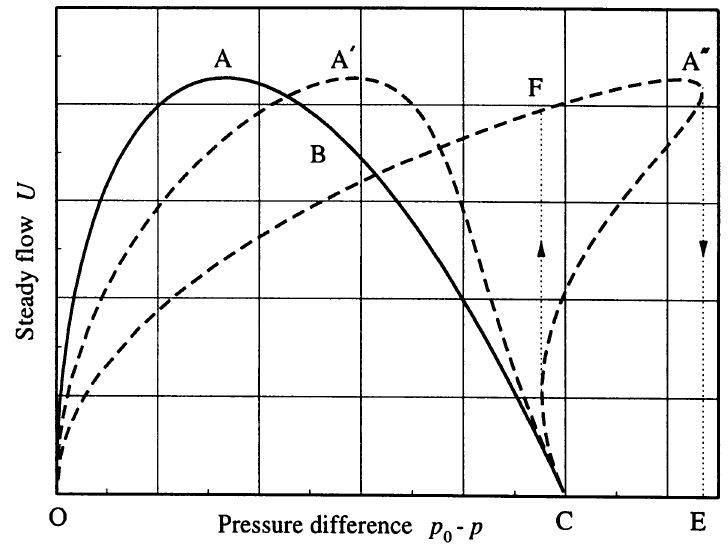
\includegraphics[width=0.7\linewidth]{00_Images/04_chapter/img109.jpg}
\caption{Effect of added flow resistance on the double-reed static characteristic}
\label{fig:double_reeds_resistance_effect}
\end{figure}

\section{Nonlinearities and Self-oscillations}

In instruments with continuous energy input, such as wind and bowed-string instruments, sound generation depends on specific conditions in the exciter-resonator interaction. A central point is that the exciter is typically governed by nonlinear dynamics, so that its input depends on its own state and on the coupled acoustic field. 

\subsection{Nonlinear Dynamic Model}

A generic nonlinear model for the exciter displacement \( y(t) \) can be written as
\[
m\ddot y + R\dot y + Ky = F(y,\dot y,t)
\]
so that the forcing depends on the output \( y \), on its time derivative, and possibly on additional external inputs. Typical examples include bowed strings, where the bow force depends on the relative velocity between bow and string, and reed instruments, where the pressure depends on the reed displacement, which is the unknown function of the differential equation. In addition, \( m \), \( R \), and \( K \) may also depend on \( y \). It is convenient to rewrite the dynamics in the normalized form
\[
\ddot y + \omega_0^2 y = g(y,\dot y,t)
\]
where \( \omega_0 \) is the linear natural frequency and \( g \) collects damping, nonlinearity, and forcing contributions.

\subsection{Slowly Varying Amplitude and Phase}

If damping, nonlinearity, and external forcing are small, the response is approximately sinusoidal,
\[
y(t) = a\sin(\omega_0 t + \phi)
\]
If \( g \neq 0 \) but remains small compared to the linear restoring term, a standard assumption is that amplitude and phase vary slowly in time,
\[
y(t) = a(t)\sin\!\bigl(\omega_0 t + \phi(t)\bigr)
\]
Differentiation yields
\[
\dot y
= \dot a \cos(\omega_0 t + \phi)
+ a(\omega_0 + \dot \phi)\cos\!\bigl(\omega_0 t + \phi(t)\bigr)
\]
A simplification is obtained by imposing the constraint
\[
\dot a \sin(\omega_0 t + \phi) + a\dot \phi \cos(\omega_0 t + \phi) = 0
\]
which leads to
\[
\dot y = a\omega_0 \cos(\omega_0 t + \phi)
\]
Substituting the assumed form for \( y \) and \( \dot y \) into the normalized equation gives
\[
a\omega_0 \dot a \cos(\omega_0 t + \phi) - a\omega_0 \dot \phi \sin(\omega_0 t + \phi) = g
\]
and combining the two relations yields evolution equations for amplitude and phase,
\[
\dot a = \frac{g}{\omega_0}\cos(\omega_0 t + \phi)
\qquad
\dot \phi = -\frac{g}{a\omega_0}\sin(\omega_0 t + \phi)
\]
Neglecting terms whose frequency is comparable with \( \omega_0 \), and retaining only the slowly varying components \( \langle \dot a \rangle \) and \( \langle \dot \phi \rangle \), the instantaneous frequency and amplitude can be expressed as
\[
\omega = \omega_0 + \langle \dot \phi \rangle
\qquad
a(t) = a(t_0) + \int_{t_0}^{t} \langle \dot a \rangle dt
\]
These relations provide a practical characterization once the state at \( t_0 \) is known.

\subsection{Duffing Oscillator}

As an instructive nonlinear example, consider a system with stiffness that changes with displacement, representing a progressively stiffer or weaker spring. In this setting, the normalized model can be interpreted as
\[
\ddot y + \omega_0^2 y = g(y,\dot y,t)
\qquad
g = f(t) - 2\alpha \dot y - \beta y^3
\]
If the external force \( f(t) \) is sinusoidal at frequency \( \omega \), the resulting frequency-amplitude response differs depending on the sign of \( \beta \). A hysteretic behavior may appear in the forced response, with jump phenomena between branches when sweeping frequency. Typical amplitude frequency responses of the Duffing oscillator are shown in figure \ref{fig:duffing_response}.

\begin{figure}[!htb]
\centering
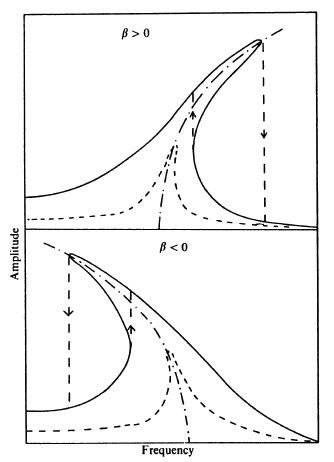
\includegraphics[width=0.6\linewidth]{00_Images/04_chapter/img118.jpg}
\caption{Duffing oscillator: forced response and hysteresis for different nonlinear stiffness signs}
\label{fig:duffing_response}
\end{figure}

\subsection{Self-excitation: Van der Pol Oscillator}

A prototypical self-excited oscillator is obtained with
\[
\ddot y + \omega_0^2 y = g(y,\dot y)
\qquad
g(y,\dot y) = a\dot y(1-y^2)
\]
No external input force is present; yet, oscillations can be sustained. In this model, the effective damping is negative for \( |y|<1 \) and positive for \( |y|>1 \), so that small-amplitude oscillations tend to grow while large-amplitude oscillations are attenuated. For sufficiently small \( a \), the oscillations remain close to sinusoidal. Examples of time histories and phase portraits for the Van der Pol oscillator are shown in figure \ref{fig:vanderpol_examples}.

\begin{figure}[!htb]
\centering
\subfloat{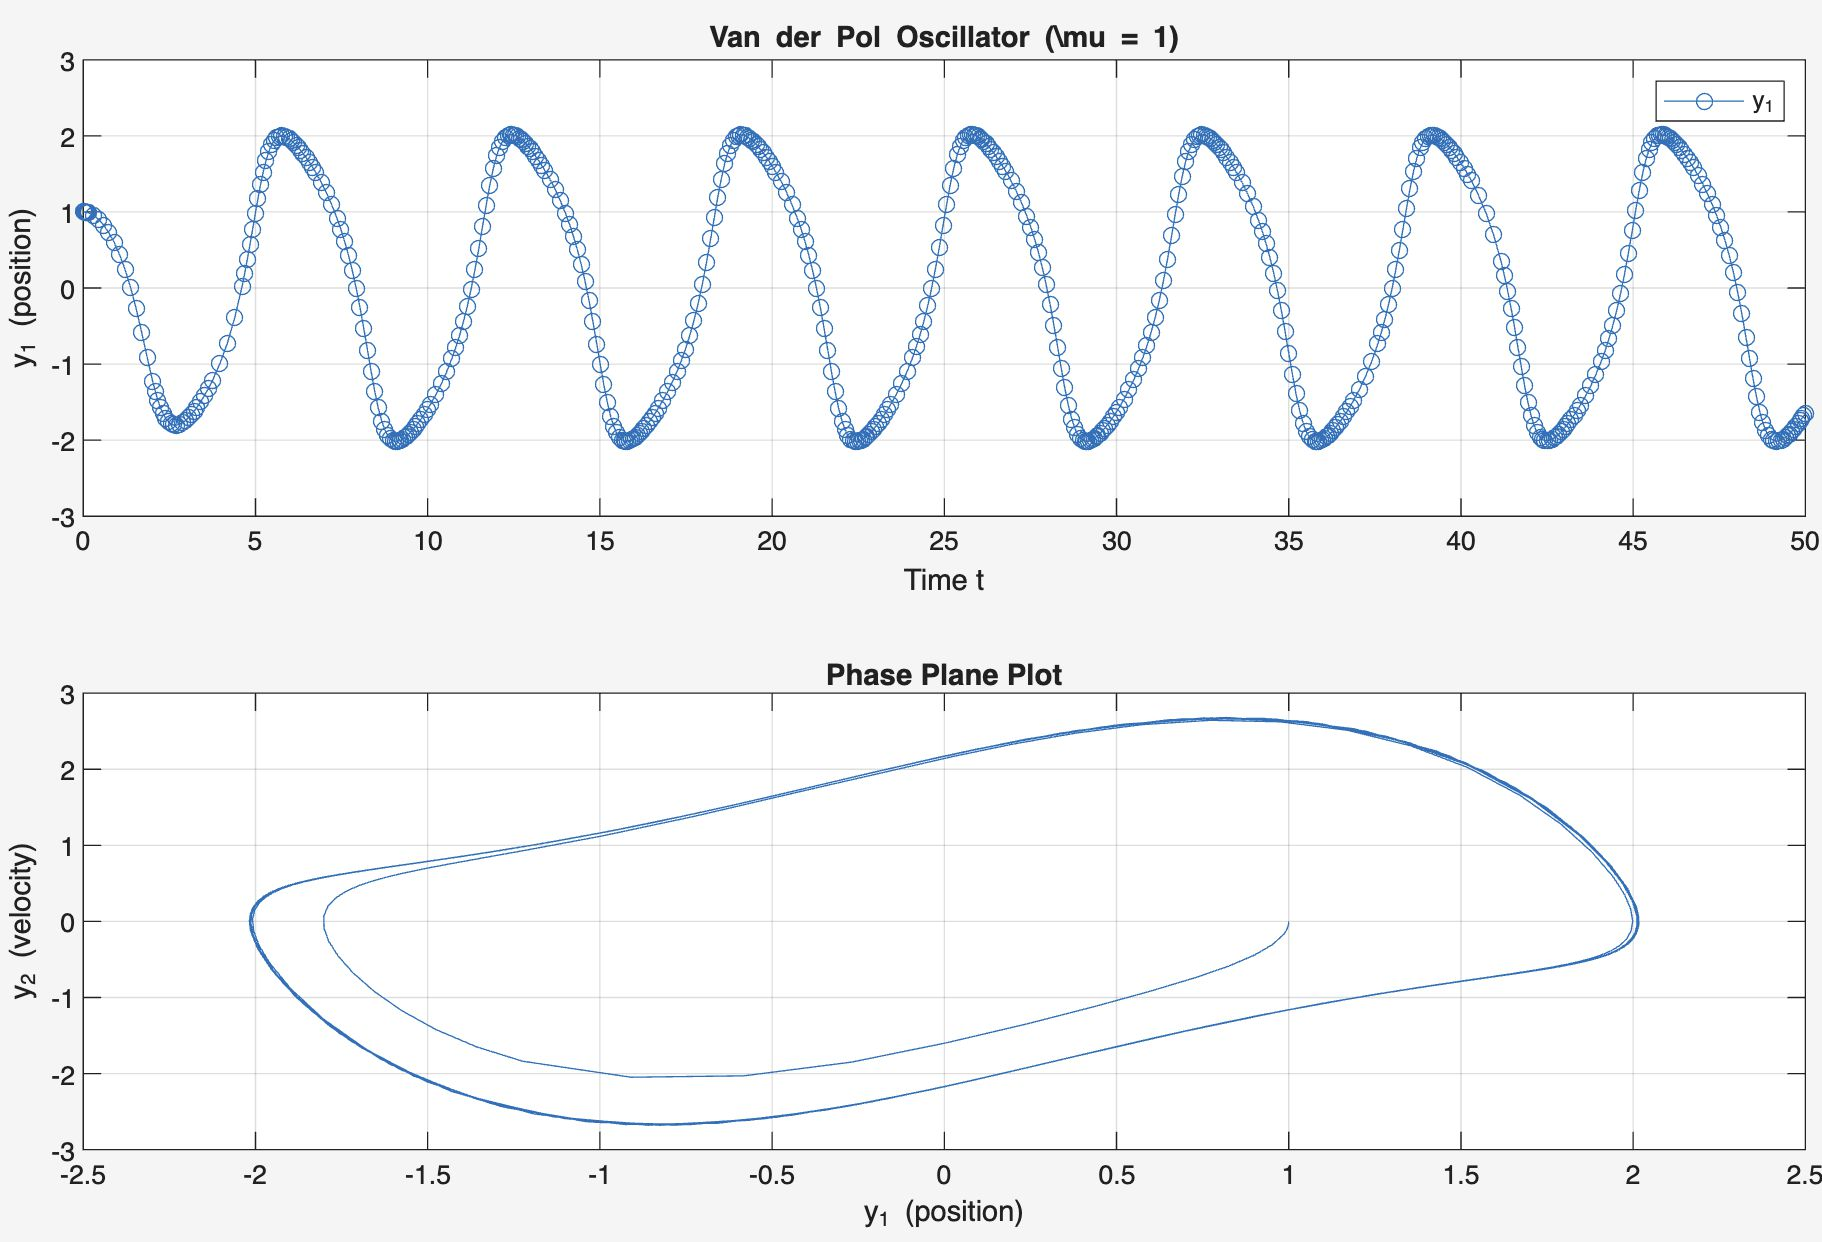
\includegraphics[width=0.45\linewidth]{00_Images/04_chapter/img125.jpg}}\hfill
\subfloat{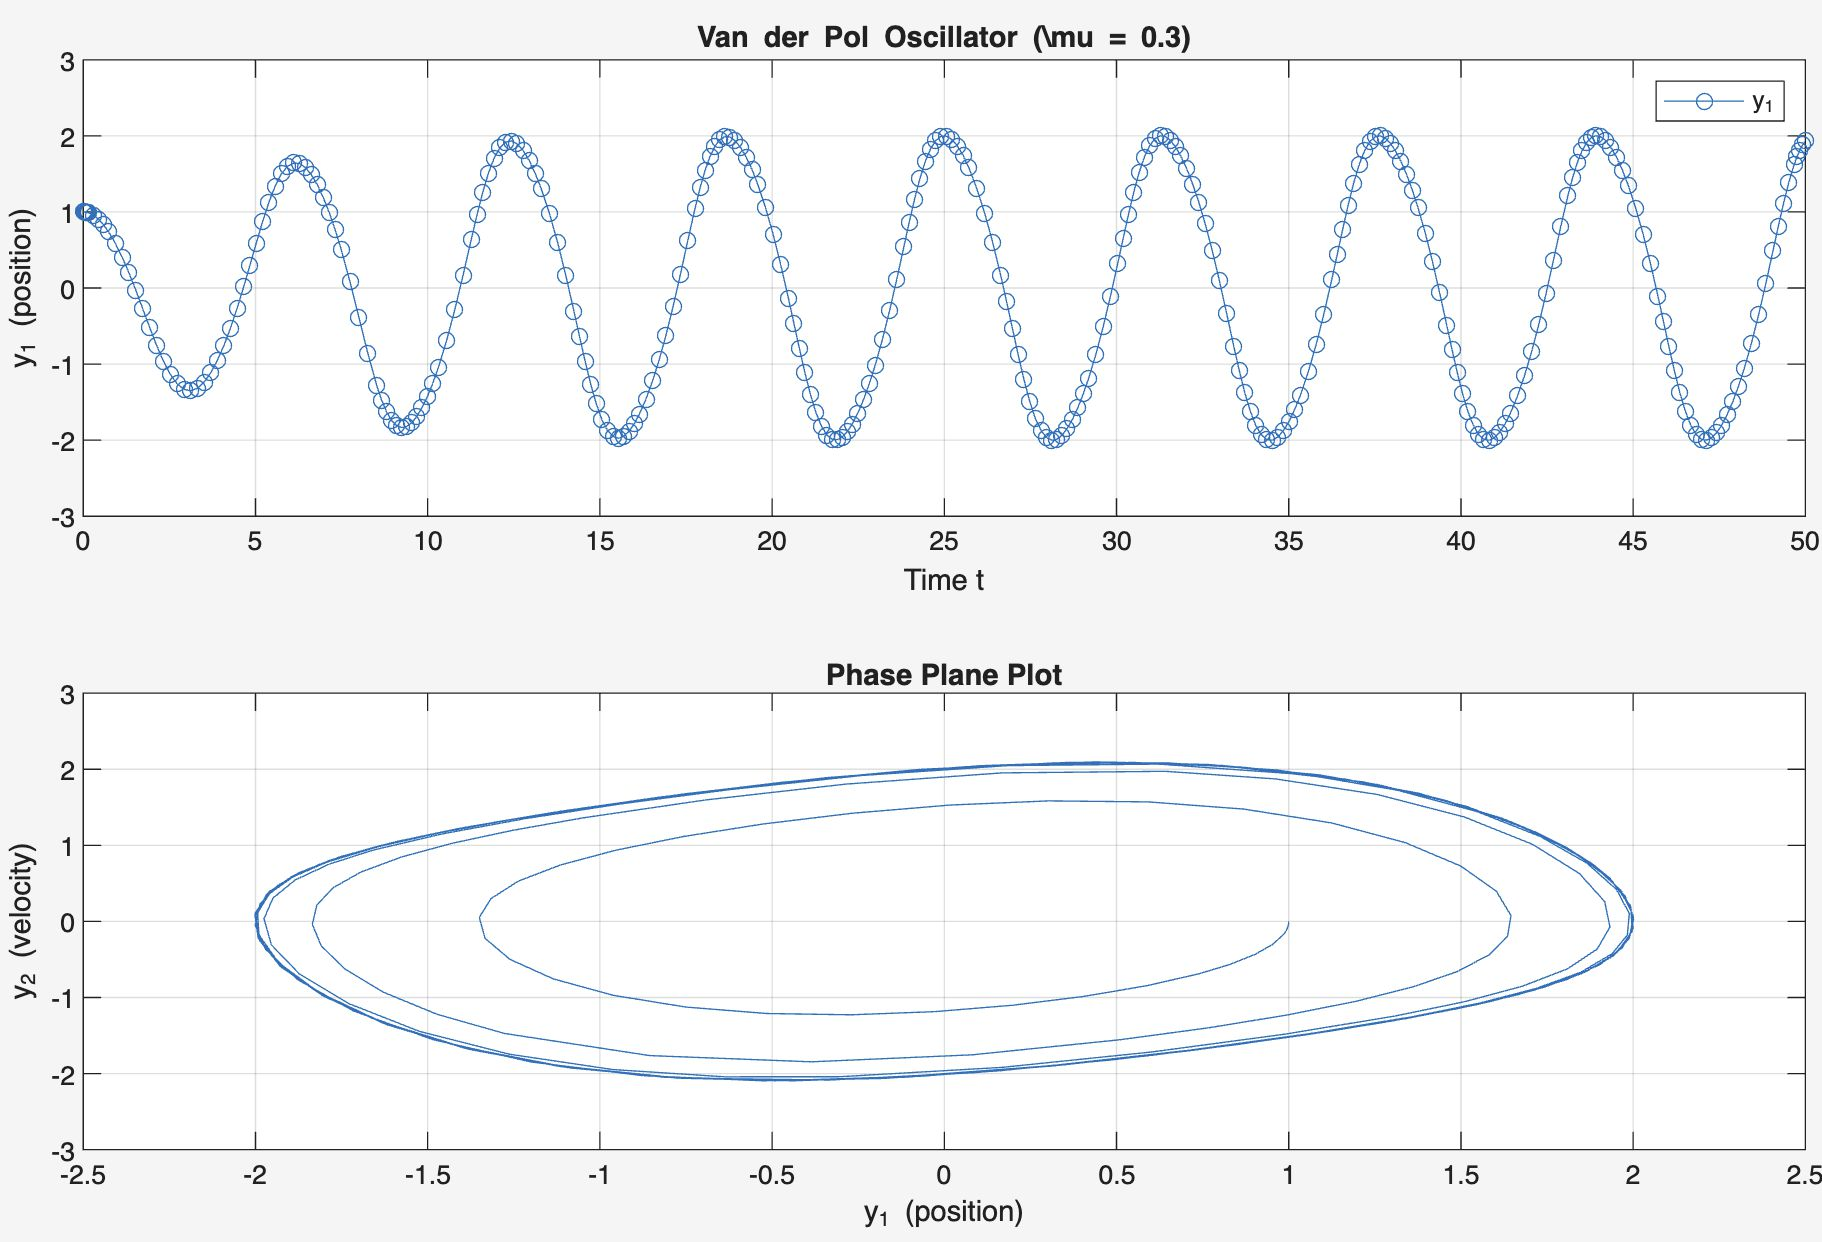
\includegraphics[width=0.45\linewidth]{00_Images/04_chapter/img127.jpg}}
\caption{Van der Pol oscillator: representative waveforms and phase portraits for two parameter settings}
\label{fig:vanderpol_examples}
\end{figure} 

\section{Reed as a Generator}

\subsection{Generator Behavior at Playing Frequency}

The quasi-static description is limited to very low frequencies. Introducing reed dynamics leads to
\[
\frac{d^2 x}{dt^2} + 2\gamma \frac{dx}{dt} + \omega_r^2 (x - x_0)
= \frac{S}{m}(\sigma_1 p_1 + \sigma_2 p_2)
\]
where \( \omega_r \) is the reed resonance frequency. The pressures \( p_1 \) and \( p_2 \) depend nonlinearly on the aperture \( x \), hence the exciter behaves as a nonlinear oscillator. The equilibrium (operating-point) opening follows from the static balance
\[
x = x_0 + (\sigma_1 p_1 + \sigma_2 p_2)\frac{S}{m\omega_r^2}
\]
At playing conditions, flow and pressure vary approximately sinusoidally around this operating point. 

\paragraph{Onset conditions} For oscillations to start, the following conditions must hold:
\[
(-,+): \ \omega < \omega_r
\qquad
X_1 + X_2 > 0
\]
\[
(+,-): \ \omega > \omega_r
\qquad
X_1 + X_2 < 0
\]
\[
(+,+): \ \frac{\omega - \omega_r}{X_1^2 - X_2^2} > 0
\qquad
X_1 - X_2 < 0
\]
where \( X_1 \) and \( X_2 \) are the reactances of the player mouth and the instrument tube, respectively. 

\subsection{Clarinet-type Reed}

For a clarinet-type reed \( (-,+) \), the playing frequency must lie below \( \omega_r \), and the total reactance must be positive. In practice, the largely negative mouth reactance must be compensated by a positive tube reactance, which requires playing sufficiently close to a tube resonance.

\subsection{Brass Instruments}

In a brass instrument played in the \( (+,-) \) configuration, the playing frequency must be above the lip resonances, and the mouth cavity compliance \( X_1 < 0 \) assists the oscillation. In the \( (+,+) \) configuration, the playing frequency will generally be below the lip and horn resonances. 

\subsection{Free Reeds}

Free reeds are a useful model for harmoniums and mouth organs. An idealized free reed consists of a curved metal tongue attached to a thin plate containing an aperture through which the tongue can just pass, and practical realizations exhibit tongue curvature and a plate of appreciable thickness. Their static flow characteristic can be represented by a curve with a preferred operating region. A schematic view of a free reed and a representative static characteristic are shown in figure \ref{fig:free_reed_scheme_characteristic}.

\begin{figure}[!htb]
\centering
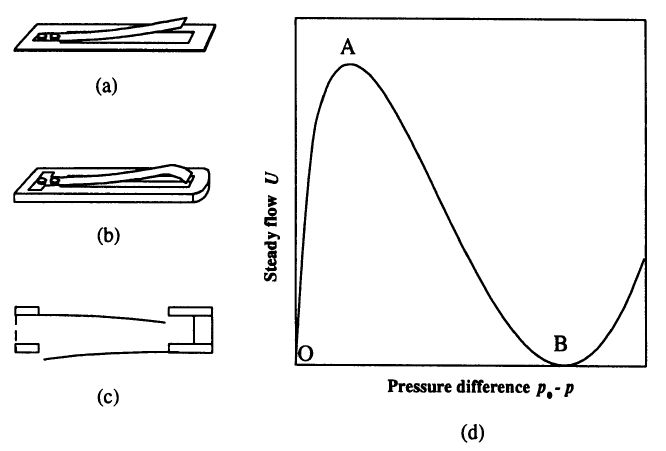
\includegraphics[width=0.8\linewidth]{00_Images/04_chapter/img142.jpg}
\caption{Free reed: geometry and representative static flow characteristic}
\label{fig:free_reed_scheme_characteristic}
\end{figure}

The playing frequency is very close to the reed resonance frequency. The best operating point lies between A and B: for a not too large pressure offset, the admittance is negative and the reed acts as a generator. If the pressure offset becomes large, the working point may move beyond B, decreasing the amplitude of the acoustic volume flow.

\subsection{Mouth Organ}

In a mouth organ, two reeds are coupled by the small air volume between them. The two reeds have opposite behaviors: one operates as \( (-,+) \) and the other as \( (+,-) \), and the resonance frequency of the closing reed is lower than that of the opening reed. When the instrument is blown, the \( (-,+) \) reed sounds, whereas the other reed produces sound when played by suction. 

\begin{figure}[!htb]
\centering
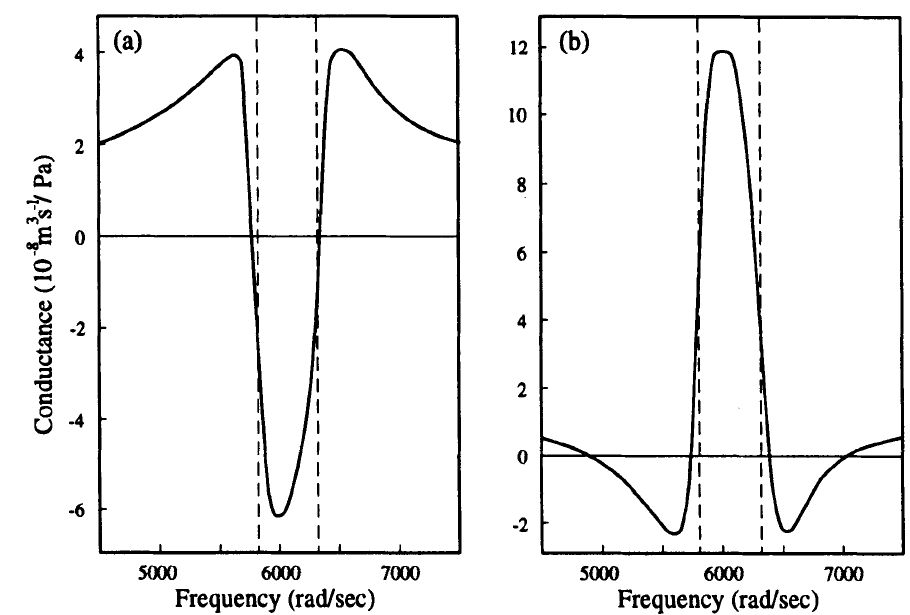
\includegraphics[width=0.8\linewidth]{00_Images/04_chapter/img157.jpg}
\caption{Pitch bending interpreted through the conductance of a coupled-reed model}
\label{fig:pitch_bending_conductance}
\end{figure}

\paragraph{Pitch bending} Pitch bending can be discussed in terms of the acoustic conductance of a coupled-reed model. The conductance behavior underlying pitch bending is illustrated in figure \ref{fig:pitch_bending_conductance}. When the resonance frequency of the closing reed is higher than that of the opening reed, pitch bending becomes possible for the closing reed. Conversely, if the resonance frequency of the closing reed is lower than that of the opening reed, the conductance behavior changes accordingly and pitch bending is not supported in the same way.

\subsection{Generators Coupled to Horns}

For an open cylindrical pipe of length \( L \) and cross-section \( S \), predominantly damped by wall losses, the input impedance can be written as
\[
Z_p = Y_p^{-1}
= \frac{\rho c}{S}
\frac{1 + jH\tan(kL)}{H + j\tan(kL)}
\]
where \( \rho \) is the density, \( c \) is the sound speed, \( k \) is the wavenumber and \( H \) is the height of the impedance maxima relative to \( \rho c/S \). The impedance maxima occur at
\[
\omega_p^{(n)} = \frac{(2n+1)\pi c}{2L}
\]
For an oscillation to grow, the overall system must operate at resonance, meaning that the overall impedance has no imaginary part and the generator overcomes the losses:
\[
\Im(Y_r) = -\Im(Y_p)
\qquad
-\Re(Y_r) > \Re(Y_p)
\]
Since \( \Im(Y_r) > 0 \) for \( (-,+) \) and \( (+,+) \) valves, one needs \( \Im(Y_p) < 0 \), implying an operating frequency slightly below the pipe resonance,
\[
\omega = \omega_p^{(n)} - \delta
\]
Conversely, for a \( (+,-) \) reed, the operating frequency must be slightly above resonance,
\[
\omega = \omega_p^{(n)} + \delta
\]

\section{Large Amplitude Behavior}

The considerations introduced previously are valid when the magnitude of the signal is small enough that a linearized version of the nonlinear reed characteristic can be used. In practice, the pressure excursion in the reed channel can be large, so the linearized characteristic is no longer informative. Even though large-amplitude regimes are generally difficult to treat, useful insights can be gained through an ab initio computation, which follows in time the progressive and regressive pressure waves in the tube and their interaction with the reed.

\subsection{Ab Initio Computation}

A convenient formulation is obtained by introducing dimensionless quantities,
\[
x^{e} = \frac{x}{H}
\qquad
p^{e} = \frac{p}{p_{C}}
\qquad
U^{e} = \frac{U Z_{c}}{p_{C}}
\qquad
Z_{c} = \frac{\rho c}{S_{P}}
\]
together with
\[
y = x^{e} + \gamma
\qquad
\gamma = \frac{p_{0}}{p_{C}}
\]
and the reed parameter
\[
\zeta = \frac{Z_{c} U(p_{A})}{p_{C}}
\]
The parameter \( \zeta \) typically lies between \( 0.3 \) and \( 0.4 \) and influences the attack transient, while the mouth pressure \( p_{0} \) dictates the amplitude and the spectrum. For notational simplicity, the superscripts are omitted in the following.

\paragraph{Progressive and regressive waves} At the pipe entrance, pressure and volume flow can be expressed in terms of progressive and regressive waves,
\[
\begin{aligned}
p &= p^{+} + p^{-} \\
U &= p^{+} - p^{-}
\end{aligned}
\qquad
\begin{aligned}
p^{+} &= \frac{1}{2}(p + U) \\
p^{-} &= \frac{1}{2}(p - U)
\end{aligned}
\]
This corresponds to a \( 45^{\circ} \) rotation of the \((p,U)\) coordinates. Since the reed characteristic provides a nonlinear relation between \( p \) and \( U \), it can be rewritten in the \((p^{+},p^{-})\) coordinates as
\[
p^{+} = G(-p^{-})
\]
where \( G \) is the reed characteristic rotated by \( 45^{\circ} \).

\paragraph{Time-domain formulation} A time-domain analysis of wave propagation in the pipe leads to
\[
p(t) = U(t) + [r \star (p + U)](t)
\]
where \( r(t) \) is the reflection function of the pipe. For a lossless pipe,
\[
r(t) = -\delta(t - \tau)
\]
so that
\[
p(t) = U(t) - p(t - \tau) - U(t - \tau)
\]
Equivalently, the lossless assumption implies
\[
p^{-}(t) = -p^{+}(t - \tau)
\]
and, at the reed,
\[
p^{+}(t) = G(-p^{-}(t)) = G(p^{+}(t - \tau))
\]

\paragraph{Iterative graphical solution} Sampling at \( t = 0, \tau, 2\tau, \ldots \) and denoting the sample index by \( n \), the wave interaction can be obtained iteratively from
\[
p^{-}_{n} = -p^{+}_{n-1}
\qquad
p^{+}_{n} = G(-p^{-}_{n}) = G(p^{+}_{n-1})
\]
A graphical iteration based on these equations yields a sequence converging to a periodic regime, and it captures the emergence of strongly non-sinusoidal waveforms. A graphical construction illustrating the iteration toward the periodic regime is shown in figure \ref{fig:graphical_iteration_solution} and the resulting mouthpiece-pressure waveform can depart strongly from sinusoidal behavior, as illustrated in figure \ref{fig:pressure_vs_square_wave}.

\begin{figure}[!htb]
\centering
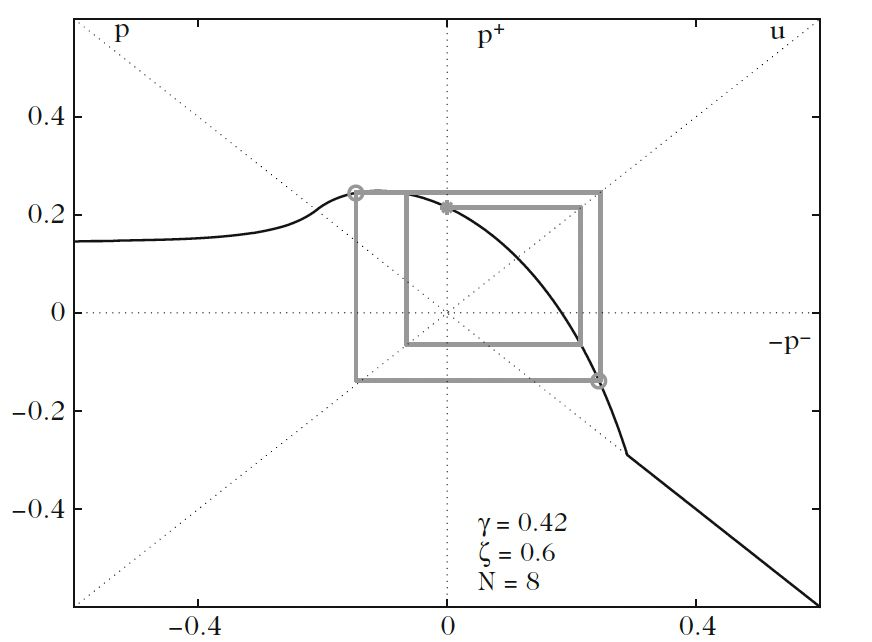
\includegraphics[width=0.6\linewidth]{00_Images/04_chapter/img168.jpg}
\caption{Graphical iteration in rotated coordinates leading to the periodic regime}
\label{fig:graphical_iteration_solution}
\end{figure}

\begin{figure}[!htb]
\centering
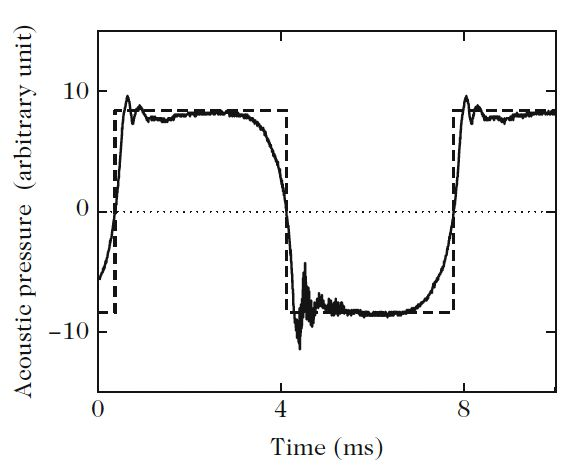
\includegraphics[width=0.6\linewidth]{00_Images/04_chapter/img174.jpg}
\caption{Large-amplitude regime: comparison between computed pressure waveform and an idealized square wave}
\label{fig:pressure_vs_square_wave}
\end{figure}

In the reported examples, increasing \( \zeta \) shortens the transient, while sufficiently small \( \gamma \) leads to convergence toward the static regime. Representative transients of pressure and volume flow for different parameter choices are shown in figure \ref{fig:transients_zeta_gamma}.

\begin{figure}[!htb]
\centering
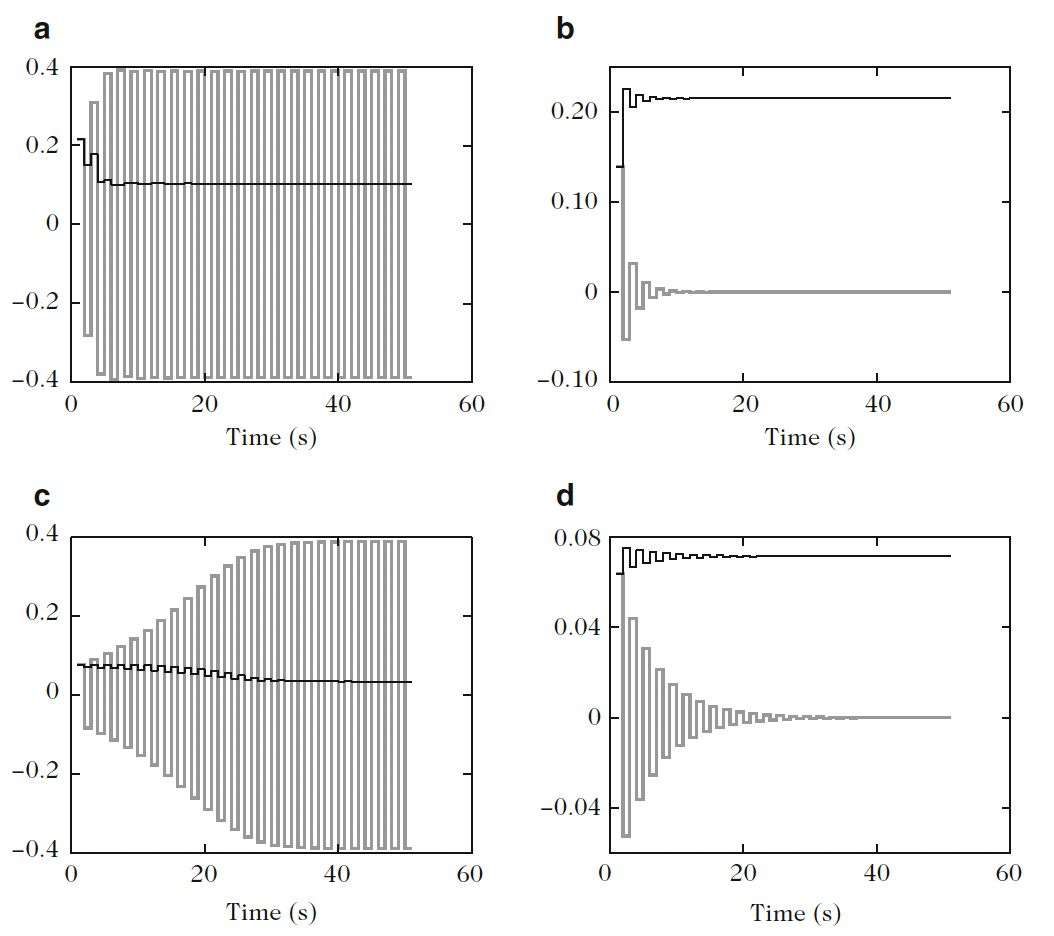
\includegraphics[width=0.7\linewidth]{00_Images/04_chapter/img180.jpg}
\caption{Attack transients of pressure and volume flow for different \(\zeta\) and \(\gamma\)}
\label{fig:transients_zeta_gamma}
\end{figure}

\subsection{Woodwind Single Reeds}

An intuitive view of the large-amplitude regime is obtained by considering the blowing pressure \( p_{0} \). In order for the mouthpiece pressure waveform to be symmetric about \( p_{0} \), the quantity \( p_{0} - p \) must have equal positive and negative excursions, which corresponds to choosing \( p_{0} \) midway between two points on the static characteristic. In this regime, the mouthpiece pressure can switch abruptly between two extreme values, while the volume flow in the two switched states is the same, apart from a finite switching transient. An illustration of switching between two extreme pressure states and the associated transient is shown in figure \ref{fig:single_reed_switching}.

\begin{figure}[!htb]
\centering
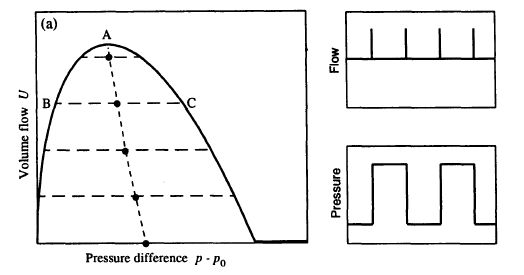
\includegraphics[width=0.7\linewidth]{00_Images/04_chapter/img192.jpg}
\caption{Single-reed large-amplitude regime: switching behavior and switching transient}
\label{fig:single_reed_switching}
\end{figure}

\paragraph{Lossy configuration and load lines} In a lossy configuration, the load lines are not horizontal. The effect of non-horizontal load lines in a lossy configuration is illustrated in figure \ref{fig:lossy_load_lines}.

\begin{figure}[!htb]
\centering
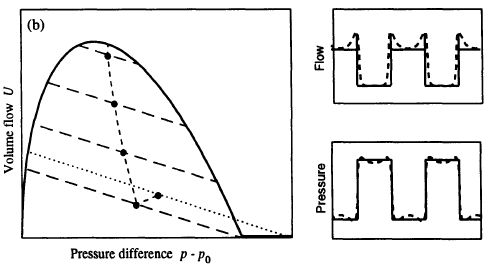
\includegraphics[width=0.7\linewidth]{00_Images/04_chapter/img197.jpg}
\caption{Lossy configuration: load lines and oscillation condition relative to the maximum negative slope}
\label{fig:lossy_load_lines}
\end{figure}

Oscillation can begin only if the load-line slope is smaller than the maximum negative slope of the reed flow characteristic. In that case, the two parts of the flow cycle have different magnitudes, producing a waveform that supplies energy to overcome the losses. Once the reed vibration reaches the beating point, the behavior changes, as indicated by a kink in the blowing-pressure curve.

\subsection{Woodwind Double Reeds}

For woodwind double reeds, the static flow is more complex because of losses in the narrow passage between the two reeds. The resulting characteristic may exhibit hysteresis. A representative hysteretic characteristic and the associated jump in operating point are shown in figure \ref{fig:double_reed_hysteresis_jump}. As the pressure rises from \( O \) to \( A^{\prime\prime} \), the admittance is positive and oscillation cannot begin. When the oscillation reaches \( A^{\prime\prime} \), the flow drops abruptly to \( C \), generating a pulse that propagates along the resonator and returns to the mouthpiece after reflection. The returning pulse lowers \( p_{0} - p \), driving the operating point to \( F \), and the cycle repeats.

\begin{figure}[!htb]
\centering
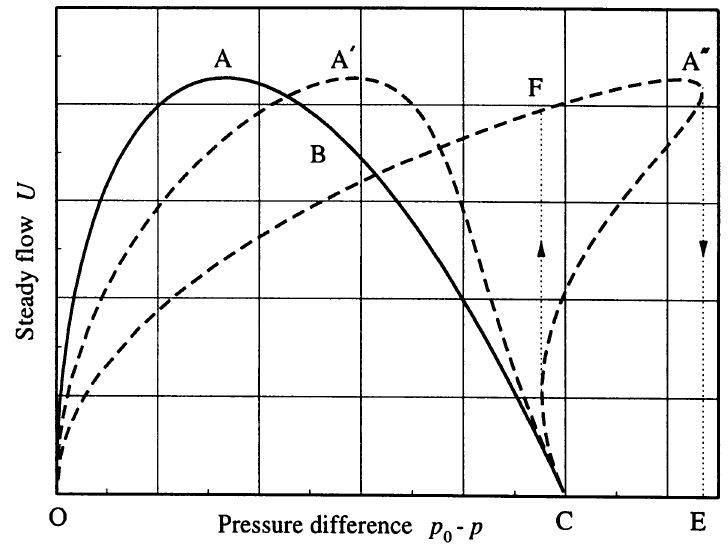
\includegraphics[width=0.7\linewidth]{00_Images/04_chapter/img202.jpg}
\caption{Double reeds: hysteresis in the static characteristic and jump from \(A^{\prime\prime}\) to \(C\)}
\label{fig:double_reed_hysteresis_jump}
\end{figure}

\subsection{Resonant Reeds and Lip Valves}

When a reed is driven at a frequency close to one of its resonances, as in the harmonium, the vibration remains essentially sinusoidal, with the notable exception of an organ pipe, where the reed can strike the shallot. Lip valves also exhibit a fairly sinusoidal behavior. The power produced by the lip generator follows a trend of the form
\[
P \propto p_{0}(p_{0} - p_{T})^{4}
\]
where \( p_{T} \) is the threshold pressure for oscillation onset. The radiated power follows a similar trend, up to losses in the instrument, and in the mid-pressure range, doubling \( p_{0} \) increases the output power by about \( \SI{15}{\decibel} \).

\subsection{Nonlinear Analysis and Harmonic Content}

The relationship between \( p \) and \( U \) is strongly nonlinear. As a consequence, an excitation at angular frequency \( \omega \) generates a flow containing components at \( n\omega \). These components enter the resonator, which behaves linearly, and generate pressure components of the form at the mouthpiece.
\[
p_{n} = Z_{p}(n\omega)U_{n}\sin(n\omega t)
\]
For a given flow, the output pressure is maximized when the system impedance is at a maximum, so instruments excited by pressure-controlled valves tend to operate at frequencies of impedance maxima. In woodwind reeds operating far from reed resonances, multiple pressure components contribute to a rich harmonic spectrum. In a saxophone, with an almost conical bore, the impedance maxima occur at \( n\omega_{1} \), so the returning pressure contains all harmonics. In a clarinet, with an open cylindrical bore, impedance maxima occur at \( (2n-1)\omega_{1} \), so the returning pressure contains only odd harmonics. When reeds operate close to a resonance, the oscillation remains nearly sinusoidal.

    %! TEX rootmain.tex

\chapter{Lip-Driven Brass Instruments}

Lip-driven brass instruments can be viewed as coupled systems in which a self-oscillating lip valve interacts with an acoustic resonator shaped like a horn. The chapter surveys how the geometry of the bore affects resonances and playing behavior, and how mouthpieces contribute to both impedance matching and control. Radiation mechanisms are then discussed, together with practical tone-shaping devices such as slides, valves, and mutes. The treatment concludes by revisiting excitation and nonlinear effects in performance conditions and by outlining less conventional design choices that deviate from standard brass-instrument archetypes.

\section{Horn Profiles}

\begin{figure}[!htb]
\centering
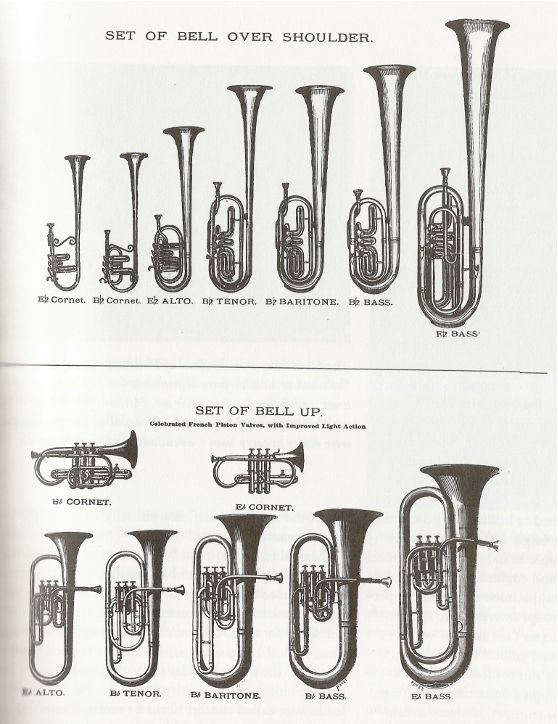
\includegraphics[width=0.5\linewidth]{00_Images/05_chapter/img34.jpg}
\caption{Overview of lip-driven brass instruments}
\label{fig:brass_overview}
\end{figure}

\subsection{Overall Geometrical Features}

Most brass instruments can be idealized as a cylindrical section connected to a flaring part. If the flaring portion is kept relatively short, for instance, not exceeding about one third of the total length, there remains enough geometrical flexibility to adjust the resonance frequencies of the modes through design choices in the profile. A reasonable approximation for many instruments, especially historical ones, is a cylindrical tube connected to a more-or-less conically expanding section of comparable length, terminated at the open end by a short region of more rapid flare. A representative overview of lip-driven brass instruments and their typical geometrical variety is shown in figure \ref{fig:brass_overview}.

\subsection{Conical Expansion And Tone}

Gently toned instruments typically exhibit a conical expansion over a large fraction of their length, up to about two thirds, with a small cone angle. In contrast, brightly toned trumpets and trombones tend to have a shorter expanding section and a more pronounced flare concentrated at the bell. For compound horns, the mode distribution is not described by a simple analytical sequence, although the series of input-impedance maxima remains more-or-less harmonic. 

\subsection{Bessel Horns}

A close approximation to the horn shape of a real brass instrument is provided by the Bessel horn model. If the mouth of the horn is located at \( x_0 \), the bore radius \( a \) as a function of the axial coordinate \( x \) is written as
\[
a = b(x - x_0)^{-\gamma}
\]
where \( \gamma \) controls the flare of the horn and \( b \) is a scaling constant. The effect of the flaring parameter on Bessel-horn profiles is illustrated in figure \ref{fig:bessel_profiles}.

\begin{figure}[!htb]
\centering
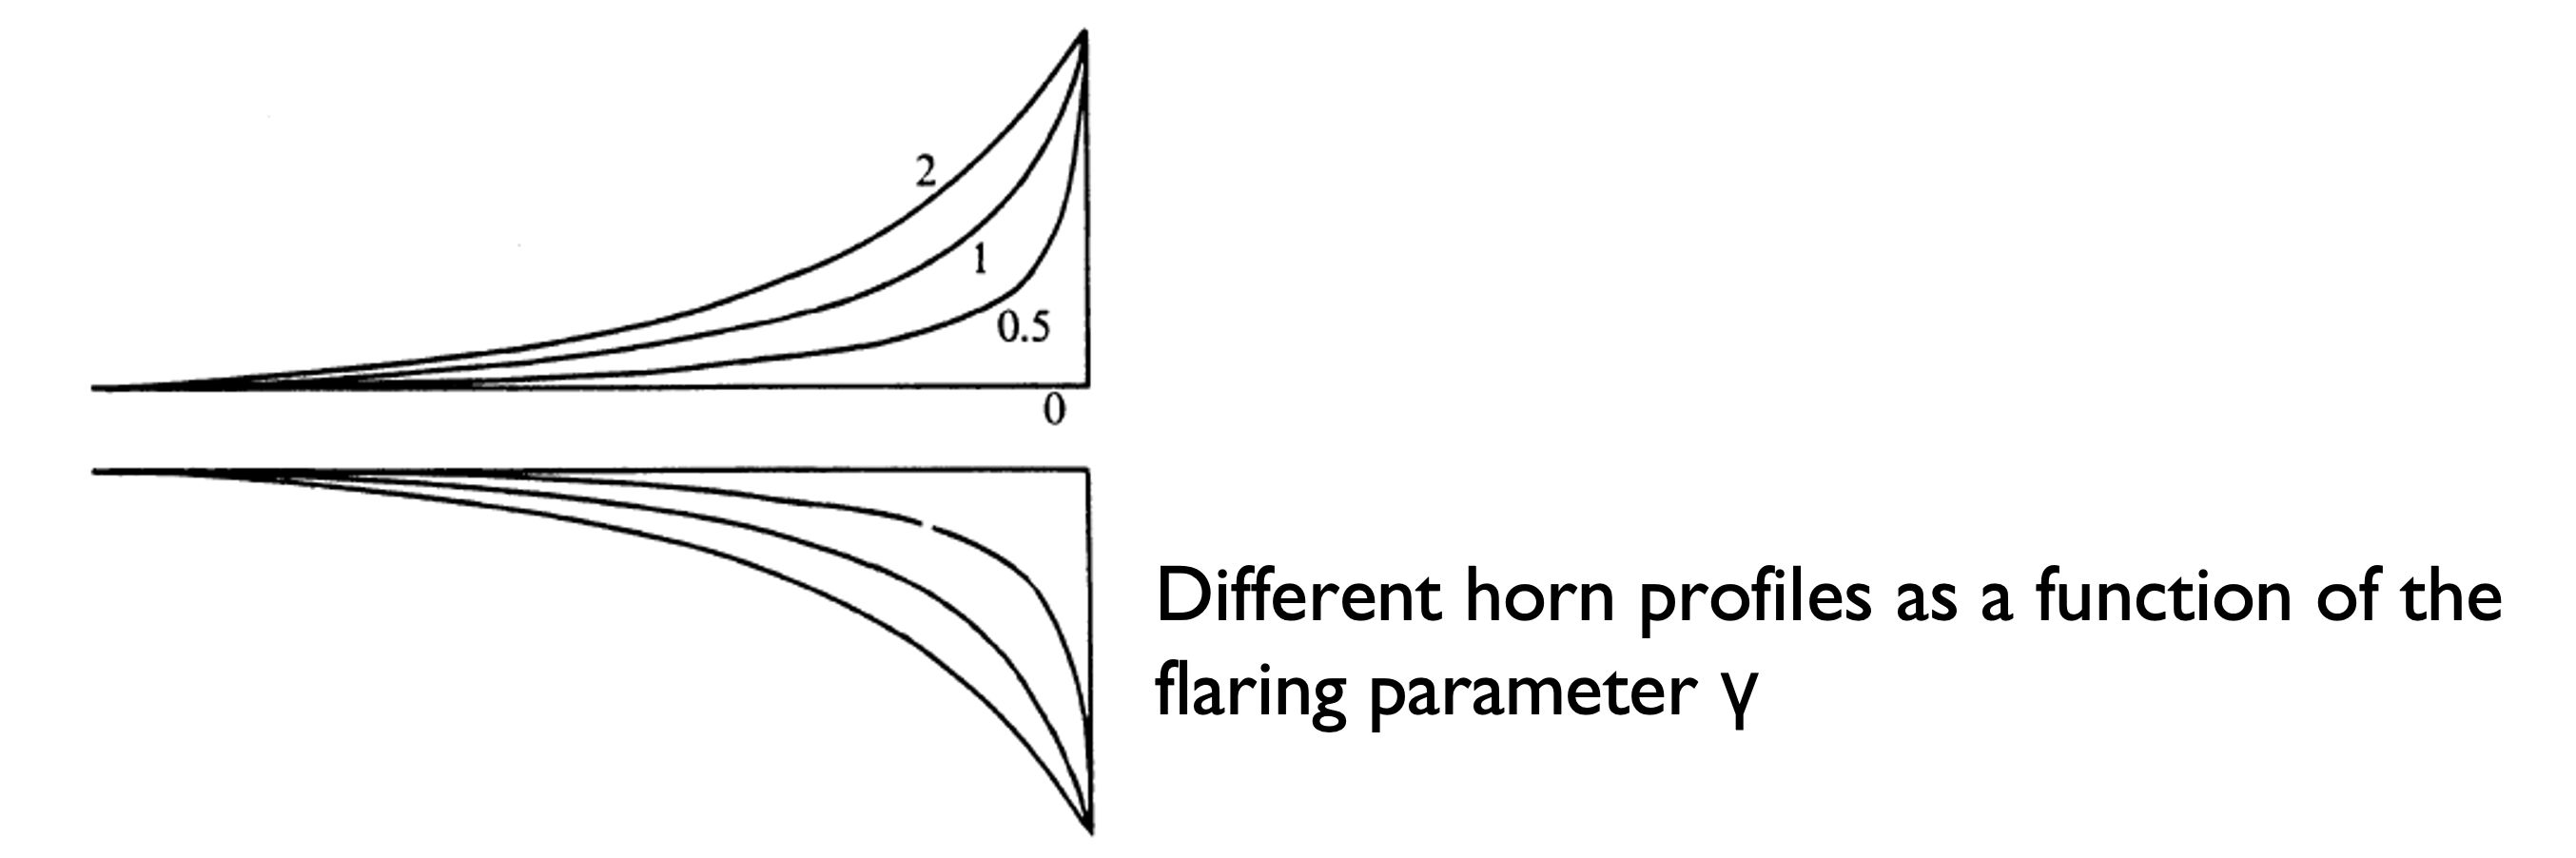
\includegraphics[width=0.7\linewidth]{00_Images/05_chapter/img79.jpg}
\caption{Bessel horn profiles for different values of the flare parameter}
\label{fig:bessel_profiles}
\end{figure}

\subsection{Impedance Maxima And Mode Series}

For a Bessel horn coupled to a tube of length \( l \), the frequencies of the impedance maxima can be approximated by
\[
f_n \approx \frac{c}{4(l + x_0)}
\left[(2n - 1) + \beta\sqrt{\gamma(\gamma + 1)}\right]
\]
where \( c \) is the sound speed and the coefficient \( \beta \) is about \( 0.6 \) for \( \gamma < 0.8 \) and about \( 0.7 \) for \( \gamma > 0.8 \). A few practical consequences follow from this description:

\begin{itemize}
    \item For \( \gamma = 1 \), the resonances are approximately harmonic, with
    \[
    f_n \approx \frac{nc}{2(l + x_0)}
    \]
    \item Instruments in the trumpet and trombone families typically correspond to \( \gamma \approx 0.7 \). Such horns can connect smoothly to cylindrical tubes, but their shape usually needs to be adjusted during design to obtain well-aligned reference resonances.
    \item The intended mode series is often tuned to approximate \( (0.7, 2, 3, 4, \dots)f_0 \). The first resonance is therefore strongly out of alignment, produces a very weak sound, and is not used in normal playing.
    \item Skilled players may nevertheless exploit nonlinear effects to produce a pedal note near \( f_0 \), relying on cooperation with the harmonically related higher resonances.
\end{itemize}

The relation between horn profile and the series of impedance maxima is illustrated in figure \ref{fig:impedance_maxima_series}.

\begin{figure}[!htb]
\centering
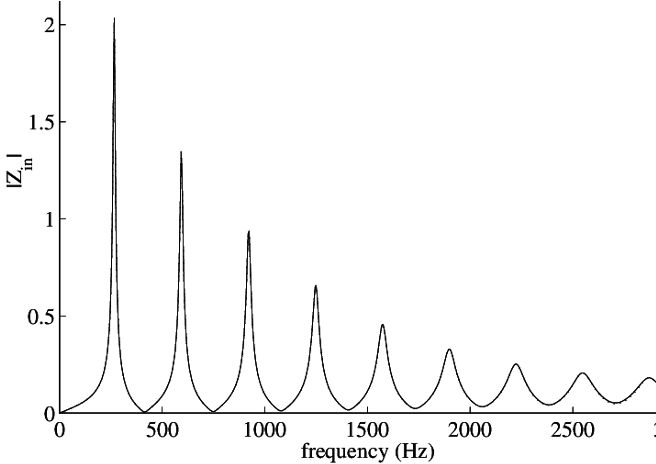
\includegraphics[width=0.7\linewidth]{00_Images/05_chapter/img93.jpg}
\caption{Impedance maxima and mode series in brass instruments}
\label{fig:impedance_maxima_series}
\end{figure}

\section{Mouthpieces}

The mouthpiece cup size roughly follows the size of the instrument as a whole. The player’s lips press against the smooth rim and cup surface, which provides comfortable mechanical support while allowing the lips to vibrate. The cup communicates with the instrument through a constricted passage (the throat), whose diameter is considerably smaller than the main bore. Mouthpieces also differ systematically across instrument families. Typical trumpet mouthpieces exhibit a relatively shallow cup and a narrow throat, while horn mouthpieces tend to have a deeper cup and a different internal contour, reflecting distinct requirements in impedance shaping and playing feel. 

\subsection{Lumped Model}

In acoustic terms, the detailed contour of the mouthpiece is less important than the cup volume and the diameter of the constricted passage. Representative mouthpiece profiles for different brass instruments are shown in figure \ref{fig:mouthpiece_profiles}.

\begin{figure}[!htb]
\centering
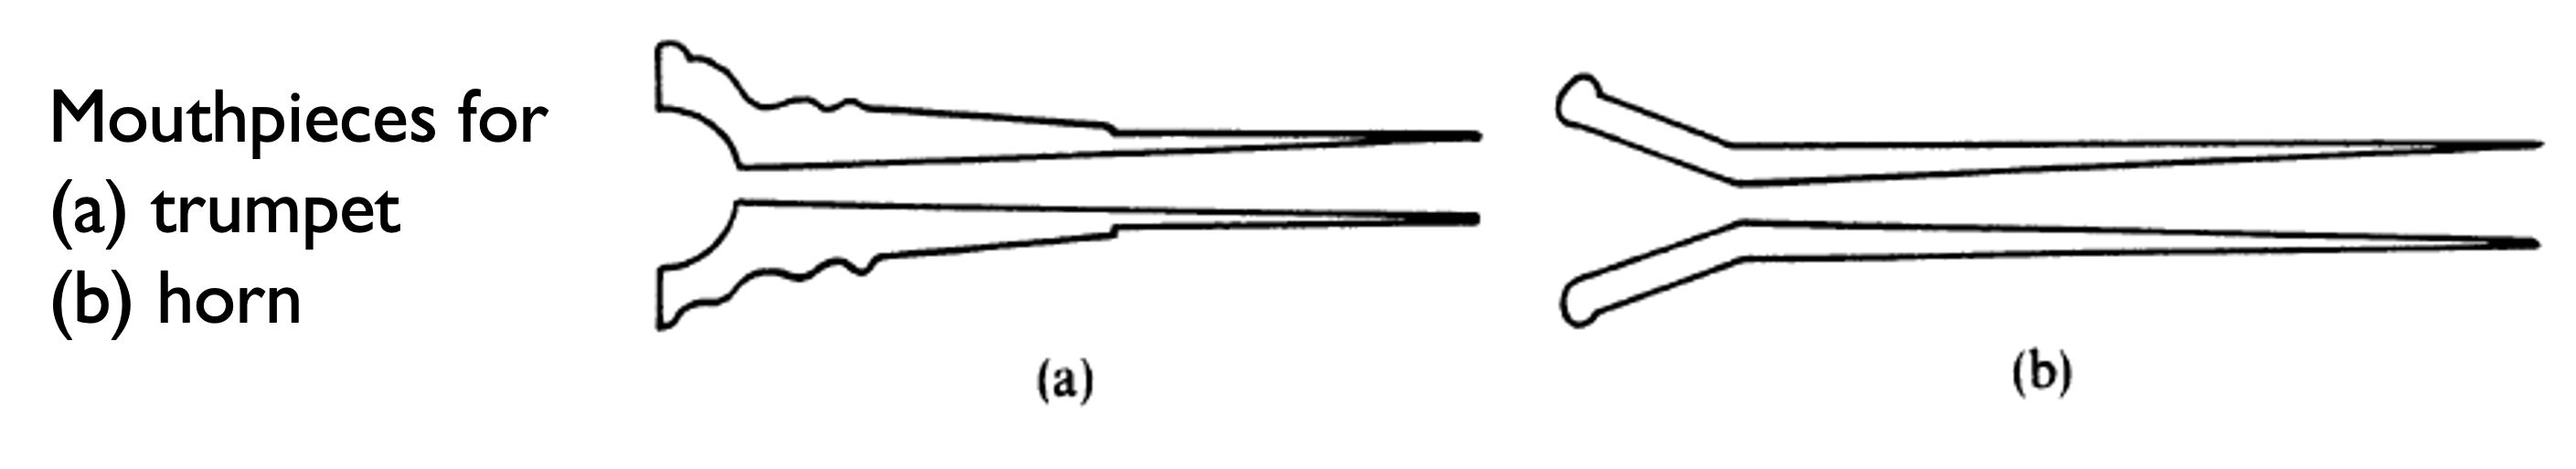
\includegraphics[width=0.7\linewidth]{00_Images/05_chapter/img103.jpg}
\caption{Mouthpiece profiles (e.g., trumpet versus horn)}
\label{fig:mouthpiece_profiles}
\end{figure}

The cup volume \( V \) acts as an acoustic compliance,
\[
C = \frac{V}{\rho c^{2}}
\]
where \( \rho \) is the air density and \( c \) is the speed of sound. The constriction behaves as a series of inertances,
\[
L = \frac{\rho l_c}{S_c}
\]
where \( S_c \) is the cross-sectional area of the constriction and \( l_c \) is its effective length. An additional dissipative element \( R \) in series with \( L \) represents viscous and thermal losses in the narrow passage.

\subsection{Coupling With The Resonator}

A convenient representation of the complete instrument is obtained through an electro acoustic analog: the cup compliance \( C \) loads the input, the constriction contributes the series elements \( L \) and \( R \), and the horn (or tube) contributes its own input impedance. A lumped (electro-acoustic) representation of the mouthpiece and its loading is shown in figure \ref{fig:mouthpiece_lumped_analog}.

\begin{figure}[!htb]
\centering
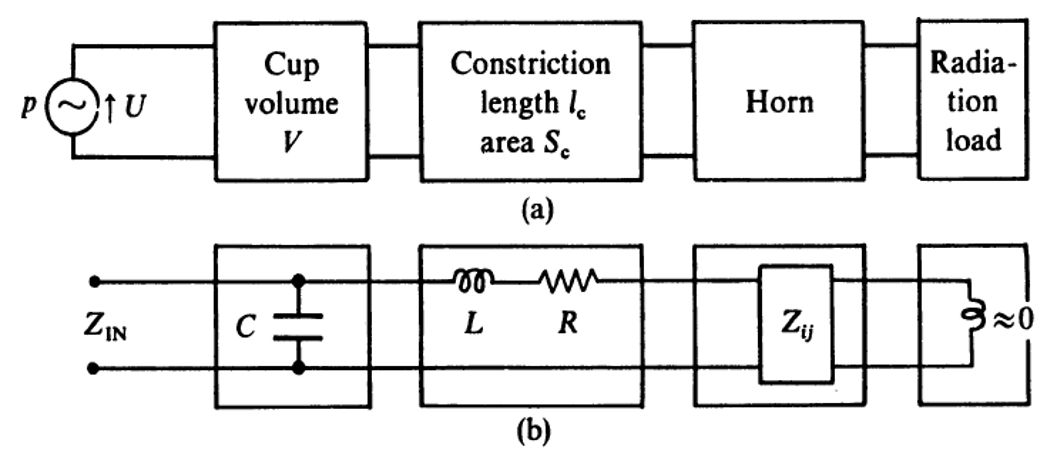
\includegraphics[width=0.7\linewidth]{00_Images/05_chapter/img117.jpg}
\caption{Lumped electro-acoustic analog of the mouthpiece and associated loads}
\label{fig:mouthpiece_lumped_analog}
\end{figure}

In this framework, the radiation impedance at the open end of the horn can be set to zero as a first approximation, since the dominant losses are attributed to wall losses along the horn. To make the coupling explicit, consider a mouthpiece connected to a simple cylindrical tube of length \( l \) and cross-sectional area \( S \). The input impedance of the tube is
\[
Z_{p} = jZ_{0}\tan(kl)
\qquad
Z_{0} = \frac{\rho c}{S}
\]
Wall losses are included by using a complex wavenumber
\[
k = \frac{\omega}{c} - j\alpha
\qquad
\alpha \approx 2\times 10^{-5}\left(\frac{\omega}{S}\right)^{1/2}
\]
with angular frequency \( \omega \). The input impedance presented to the player’s lips is then
\[
Z_{\mathrm{in}} =
\frac{R + Z_{p} + j\omega L}
{1 - \omega^{2}LC + j\omega C(R + Z_{p})}
\]
This expression highlights that the overall input impedance contains contributions associated with the tube and the mouthpiece itself. In particular, the mouthpiece behaves as a Helmholtz resonator, with a peak driving-point impedance near
\[
\omega_{0} = (LC)^{-1/2}
\]
while the peak height and half-width are controlled by the magnitude of the losses in the tube. 

\subsection{Considerations}

A few design consequences follow from the coupled model.

\begin{itemize}
    \item The lip generator is a pressure-controlled system that functions best when working with very high impedance. This motivates matching the mouthpiece to the instrument so that the mouthpiece resonance reinforces impedance peaks over the main playing range.
    \item The mouthpiece impedance also influences, to a smaller extent, the tuning of the horn resonances.
    \item The balance of resonance peak heights over the playing range is important because an easy transition between successive resonances is required for musical flexibility.
\end{itemize}

For a \( (+,-) \) lip valve, the imaginary part of the lip valve admittance is always negative. Therefore, for exact resonance and maximum acoustic pressure in the mouthpiece, the instrument must present a balancing positive acoustic admittance at the open face of the mouthpiece cup. More generally, for a multi-mode passive resonator, the imaginary part of the impedance rises through zero as the frequency passes through each impedance maximum. To satisfy the resonance condition, the operating frequency must lie slightly above the passive resonance frequency of the mode in question. The opposite conclusion applies for a valve in the \( (+,+) \) configuration. Typical impedance curves for the pipe alone, the mouthpiece alone, and the coupled system are shown in figure \ref{fig:impedance_coupling}.

\begin{figure}[!htb]
\centering
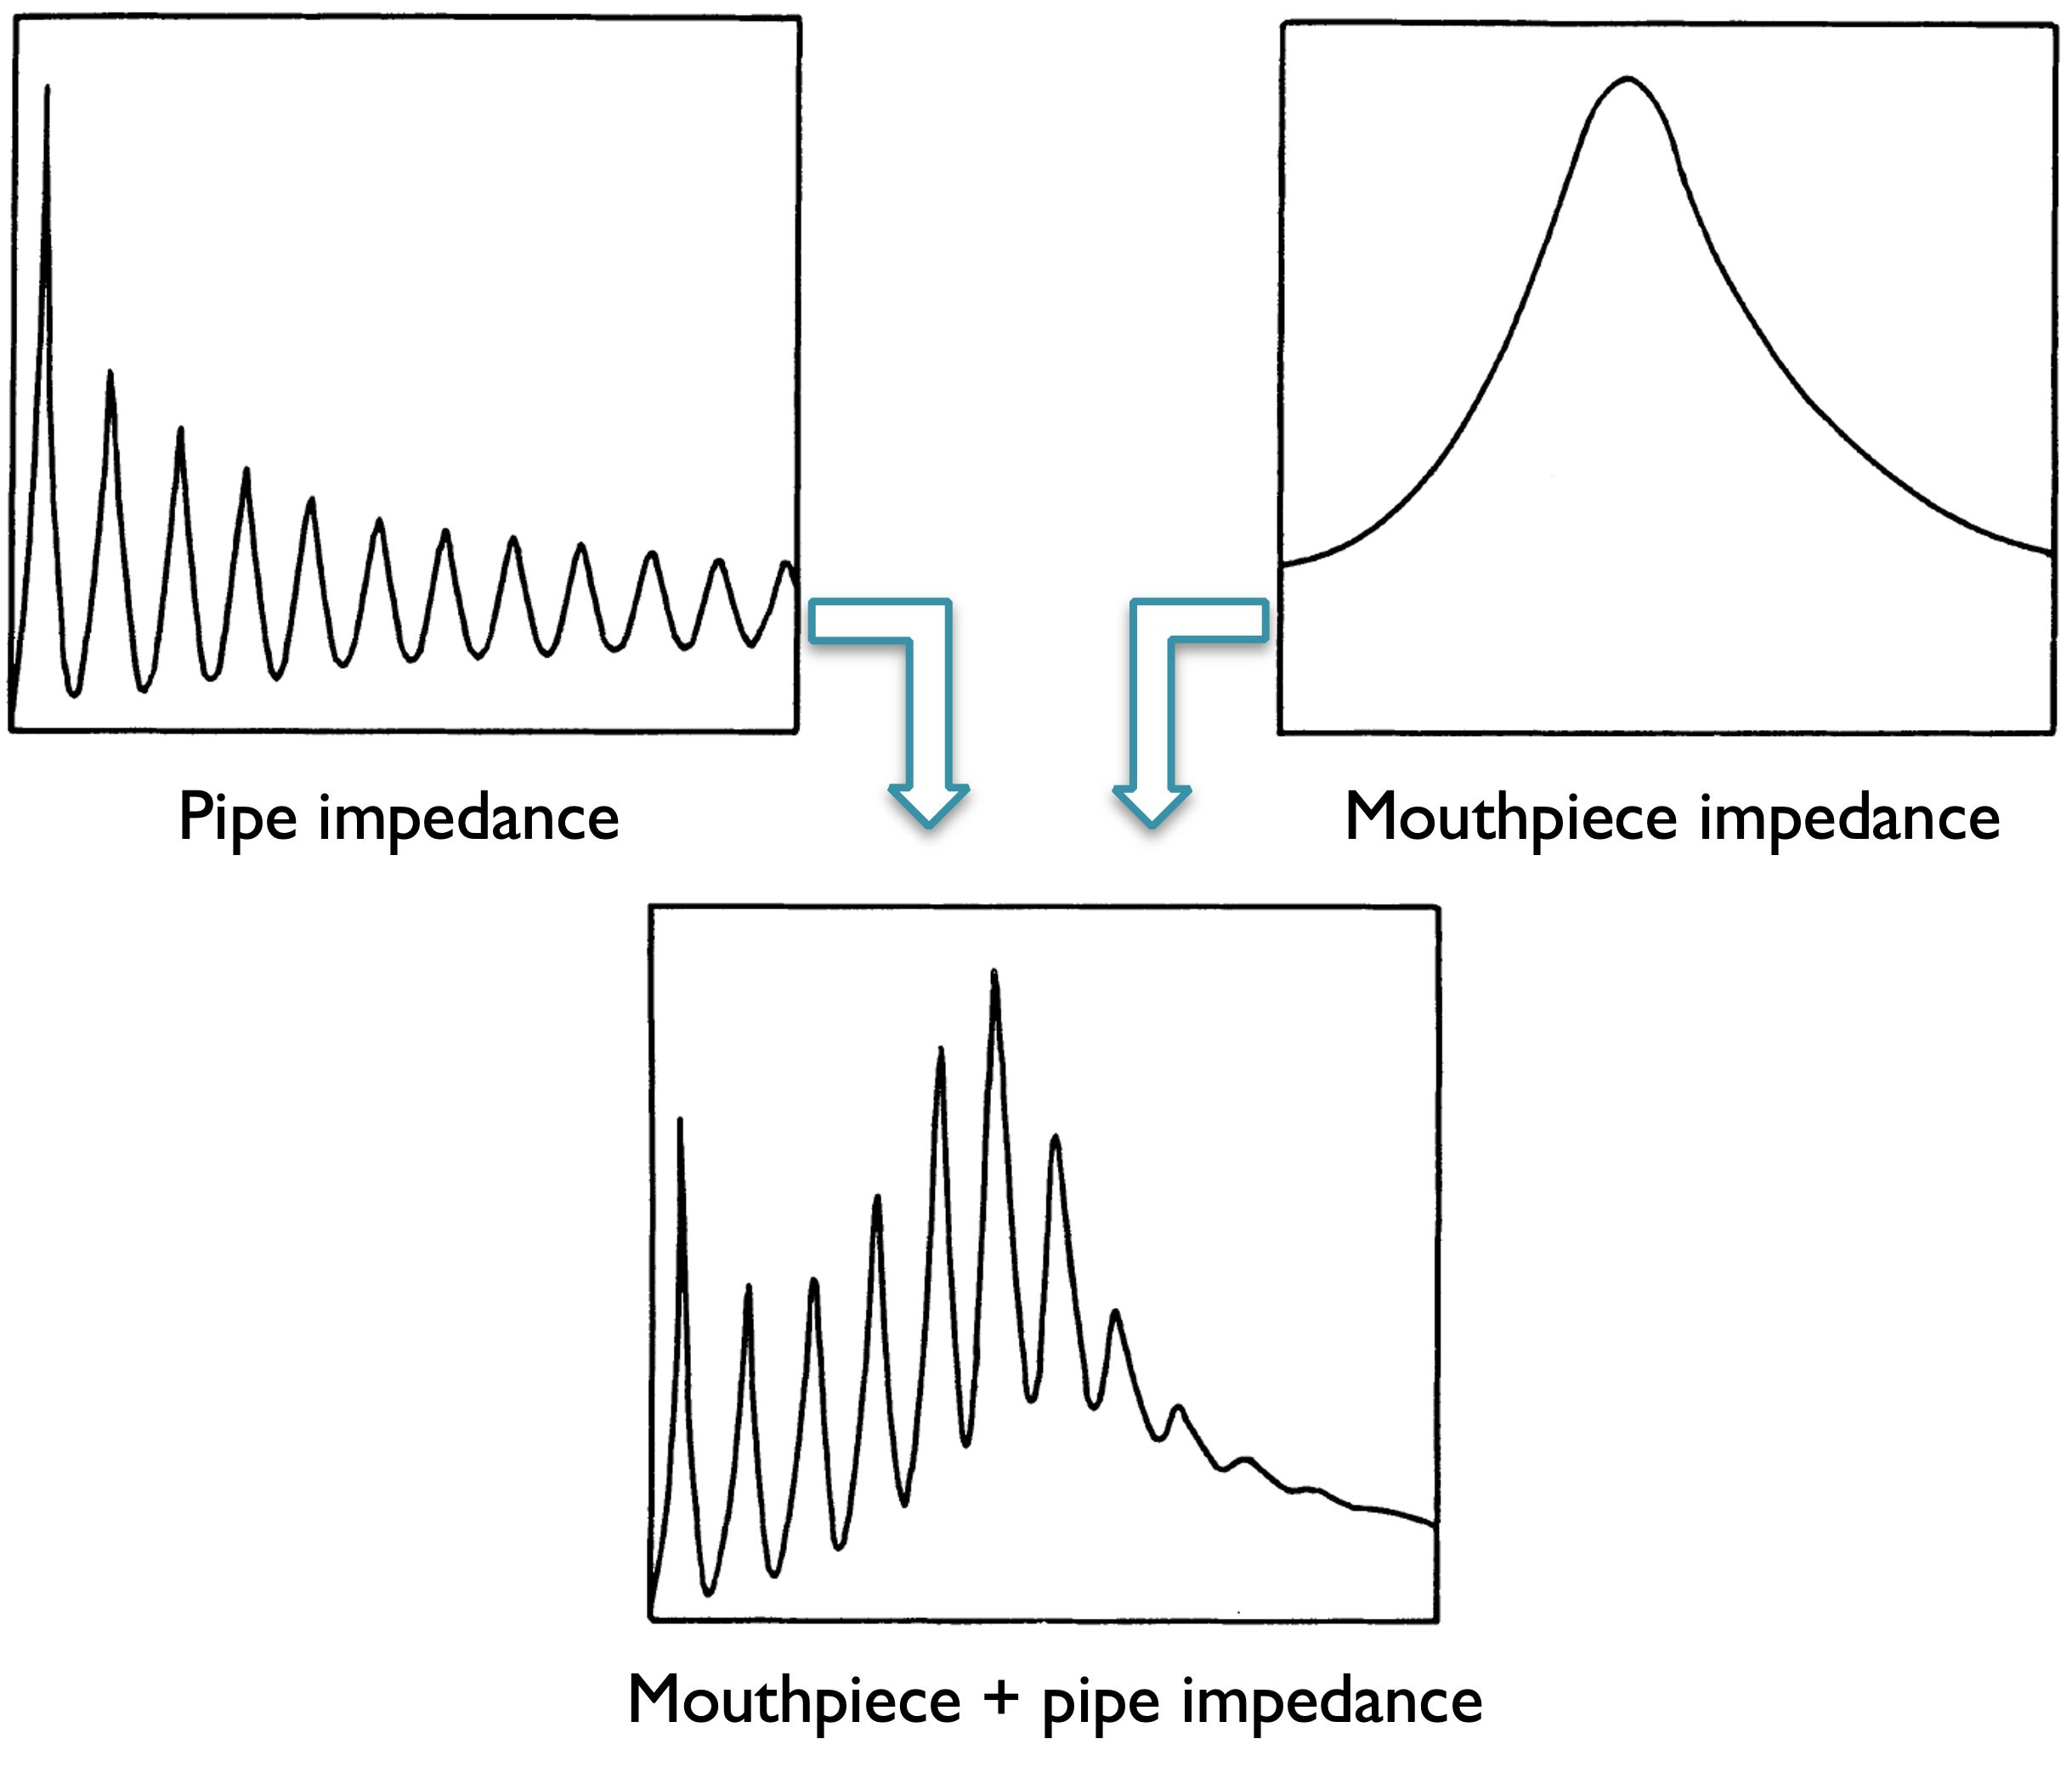
\includegraphics[width=0.7\linewidth]{00_Images/05_chapter/img125.jpg}
\caption{Impedance of pipe, mouthpiece, and coupled system}
\label{fig:impedance_coupling}
\end{figure}

\section{Radiation}

\subsection{Radiated Power}

At the horn mouth, radiation can be described through the radiation impedance \( Z_{\mathrm{rad}} \), whose resistive part \( R \) controls the radiated acoustic power. For a circular opening of radius \( a \), using \( k \) as the wavenumber and \( Z_{0} \) as the characteristic impedance associated with the mouth, the resistive term can be approximated as
\[
R \approx
\begin{cases}
Z_{0}\dfrac{(ka)^{2}}{4} & \text{for } ka \le 2 \\
Z_{0} & \text{for } ka \ge 2
\end{cases}
\]
If the acoustic particle velocity at the mouth is \( u \), the volume flow is
\[
U = \pi a^{2}u
\]
The total radiated power follows the corresponding asymptotic behaviors
\[
P \approx
\begin{cases}
\rho c\left(\pi a^{2}u^{2}\right)\dfrac{(ka)^{2}}{4} & \text{for } ka \le 2 \\
\rho c\left(\pi a^{2}u^{2}\right)(ka)^{2} & \text{for } ka \ge 2
\end{cases}
\]
These relations show that radiation efficiency increases with frequency in the low-frequency range. 

\subsection{Radiation Spectrum}

The radiation process can be viewed as a frequency-dependent transfer function: at low frequencies (relative to the cut-off), radiation is inefficient and the transfer magnitude increases with frequency, while above the cut-off it tends toward a flatter behavior. This trend is commonly summarized by plotting the transfer function versus frequency normalized to the cut-off frequency. A representative radiation spectrum (or radiation transfer) is shown in figure \ref{fig:radiation_spectrum_brass}.

\begin{figure}[!htb]
\centering
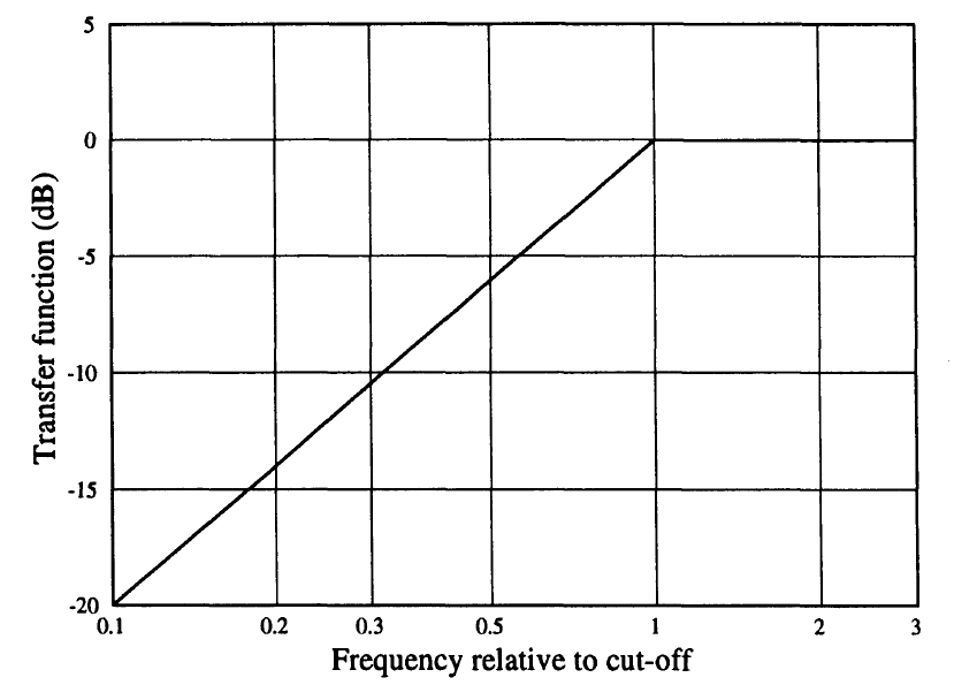
\includegraphics[width=0.7\linewidth]{00_Images/05_chapter/img133.jpg}
\caption{Radiation spectrum / transfer characteristics of a brass instrument}
\label{fig:radiation_spectrum_brass}
\end{figure} 

\subsection{Angular Dependency}

A useful directivity model is that of a baffled piston. The radiation intensity at angle \( \theta \) can be written as 
\[
\left[\frac{2J_{1}(ka\sin\theta)}{ka\sin\theta}\right]^{2}
\]
where \( J_{1} \) is the Bessel function of the first kind of order one. At low frequencies, the angular distribution is almost independent of \( \theta \). As frequency increases, radiation becomes progressively concentrated in the forward direction, and an intensity null appears at
\[
\theta_{0} = \sin^{-1}\left(\frac{3.8}{ka}\right)
\]
A practical rule is that frequencies above roughly \( 200/a \) are strongly concentrated along the horn axis. 

\section{Slides and Valves}

Slides and valves are used to fill the gaps between the lower resonances in order to produce a complete range of notes in the lower compass. 

\begin{itemize}
    \item Natural horns and Baroque trumpets did not include slides or valves. Apart from an extension shank or crook inserted between the mouthpiece and the instrument, the overall pitch could only be shifted to play in a different key. 
    \item A complete scale was therefore available only in the upper register, where adjacent resonances become sufficiently close.
    \item Additional mechanisms were needed to overcome this limitation and access intermediate notes in the lower range.
\end{itemize}

\subsection{Slides}

Ignoring the pedal note, the largest gap to be filled is between the second and third modes, which form a musical fifth and leave six notes in between. Since the frequency ratio of these modes is \( 2:3 \), covering the gap requires changing the effective tube length by about \( 50\% \),
\[
L' \approx \frac{3}{2}L
\]
because resonance frequencies scale approximately as \( f \propto 1/L \). A concrete example is provided by the tenor trombone. When the slide is closed, the bore length is approximately \SI{270}{\centi\meter} and
\[
f_2 \approx \SI{127}{\hertz}
\]
When the slide is fully open, the length increases to about \SI{405}{\centi\meter}, leading to
\[
f_2 \approx \SI{84}{\hertz}
\qquad
f_3 \approx \SI{127}{\hertz}
\]
so that the frequency region between \( f_2 \) and \( f_3 \) can be covered continuously by moving the slide. The main drawback is the large physical movement required between notes, which restricts execution speed and makes a true legato, without an audible gliding tone, nearly impossible. A typical tuning-slide arrangement is shown in figure \ref{fig:tuning_slide}.

\begin{figure}[!htb]
\centering
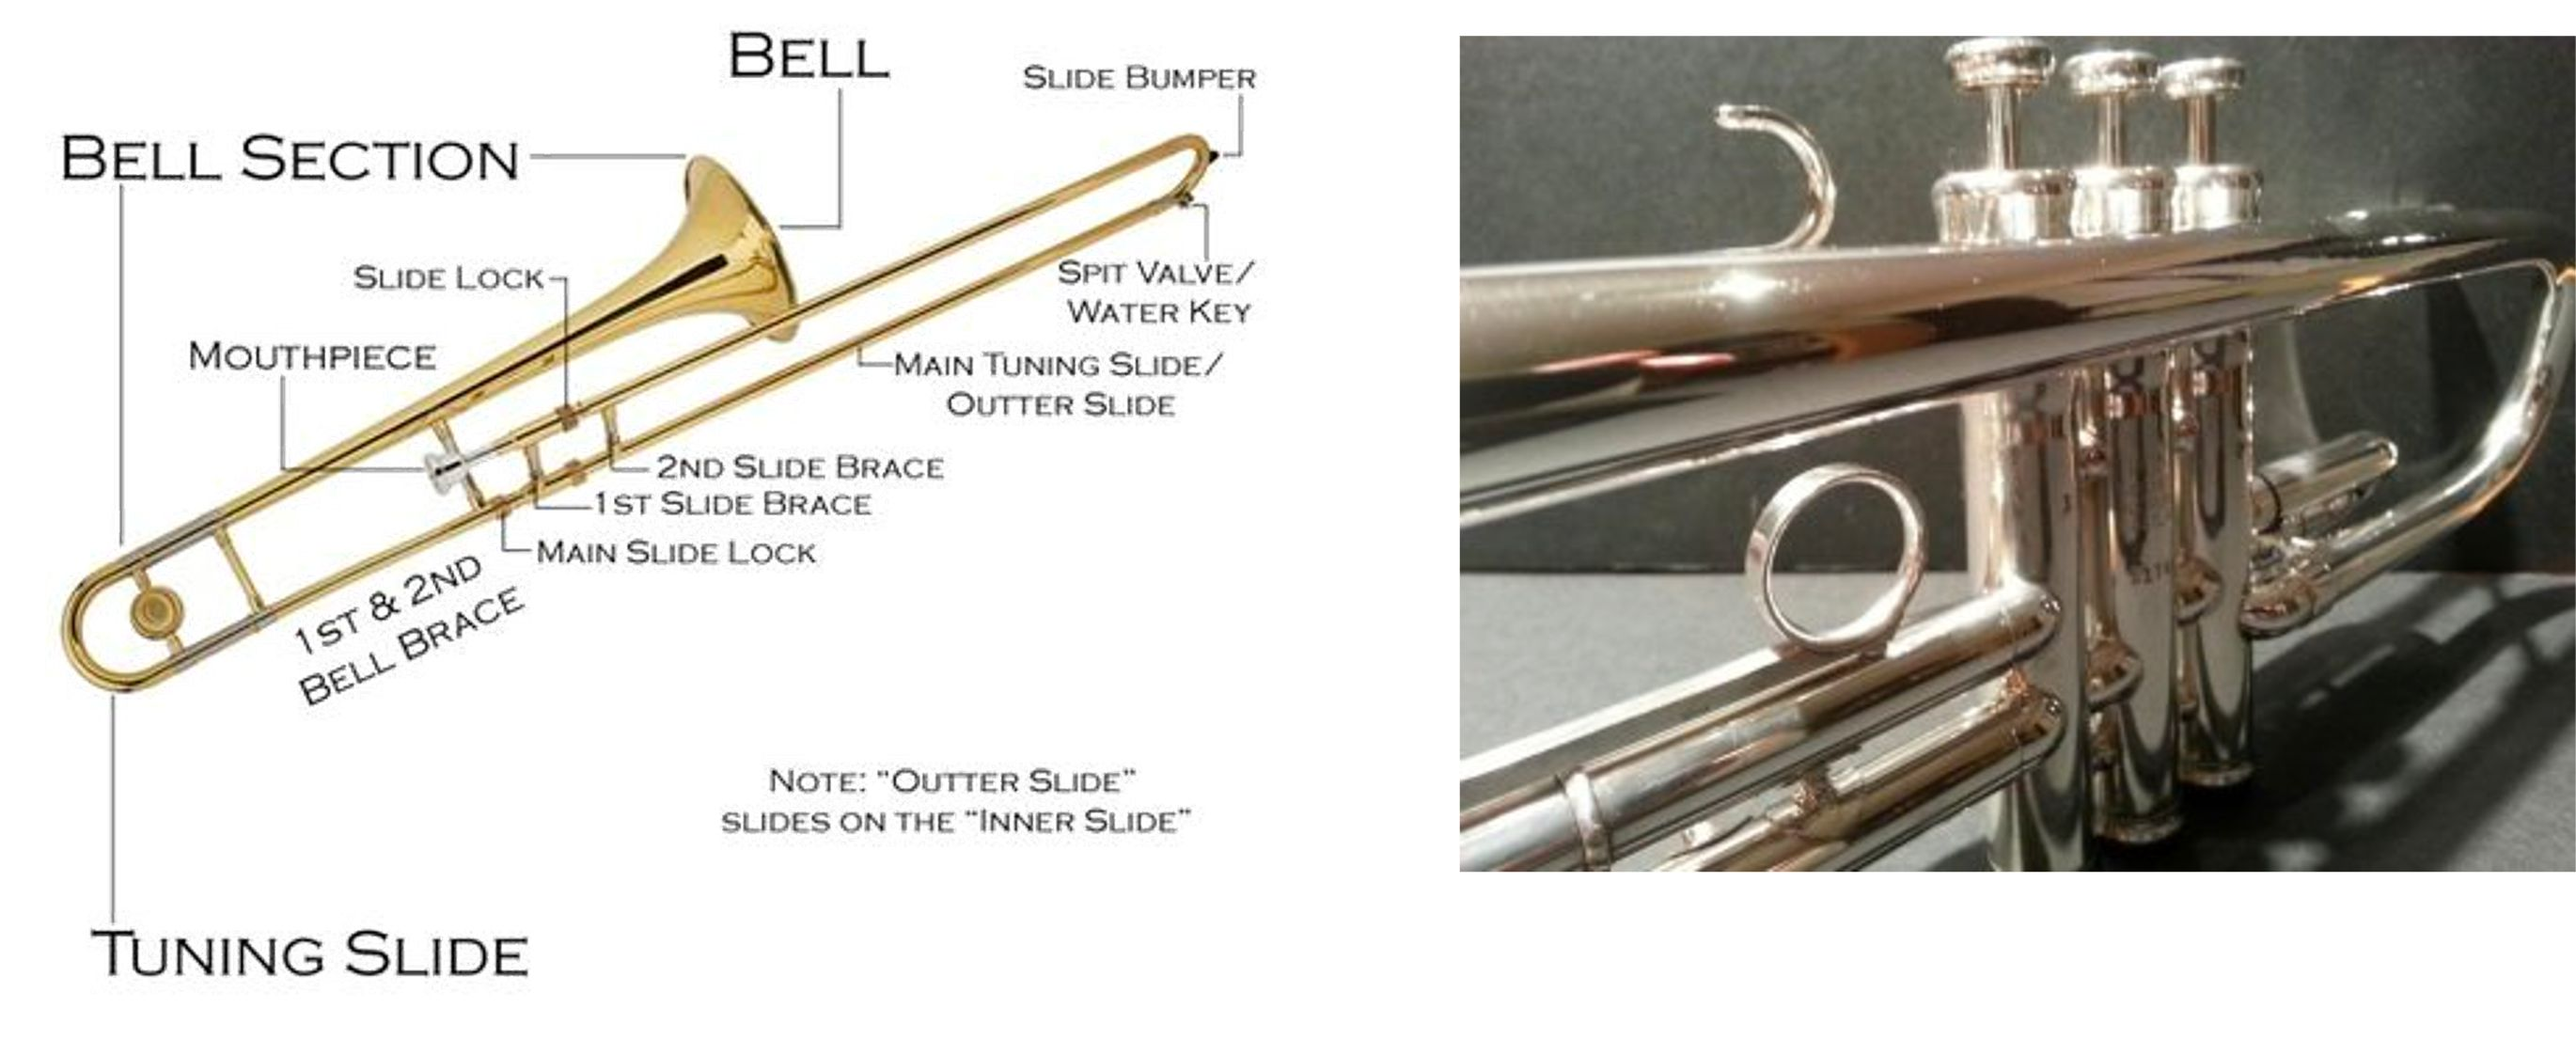
\includegraphics[width=0.7\linewidth]{00_Images/05_chapter/img141.jpg}
\caption{Tuning slide arrangement in brass instruments}
\label{fig:tuning_slide}
\end{figure}

\subsection{Valves}

The most widely adopted alternative to slides uses finger-operated valves to insert extra lengths of tubing into the cylindrical part of the instrument. Since each valve provides only two positions, at least three valves are needed, used in combination, to supply the six intermediate notes required to fill the large gap between modes 2 and 3. The operating principle and common valve configurations are illustrated in figure \ref{fig:valves_principle}.

\begin{figure}[!htb]
\centering
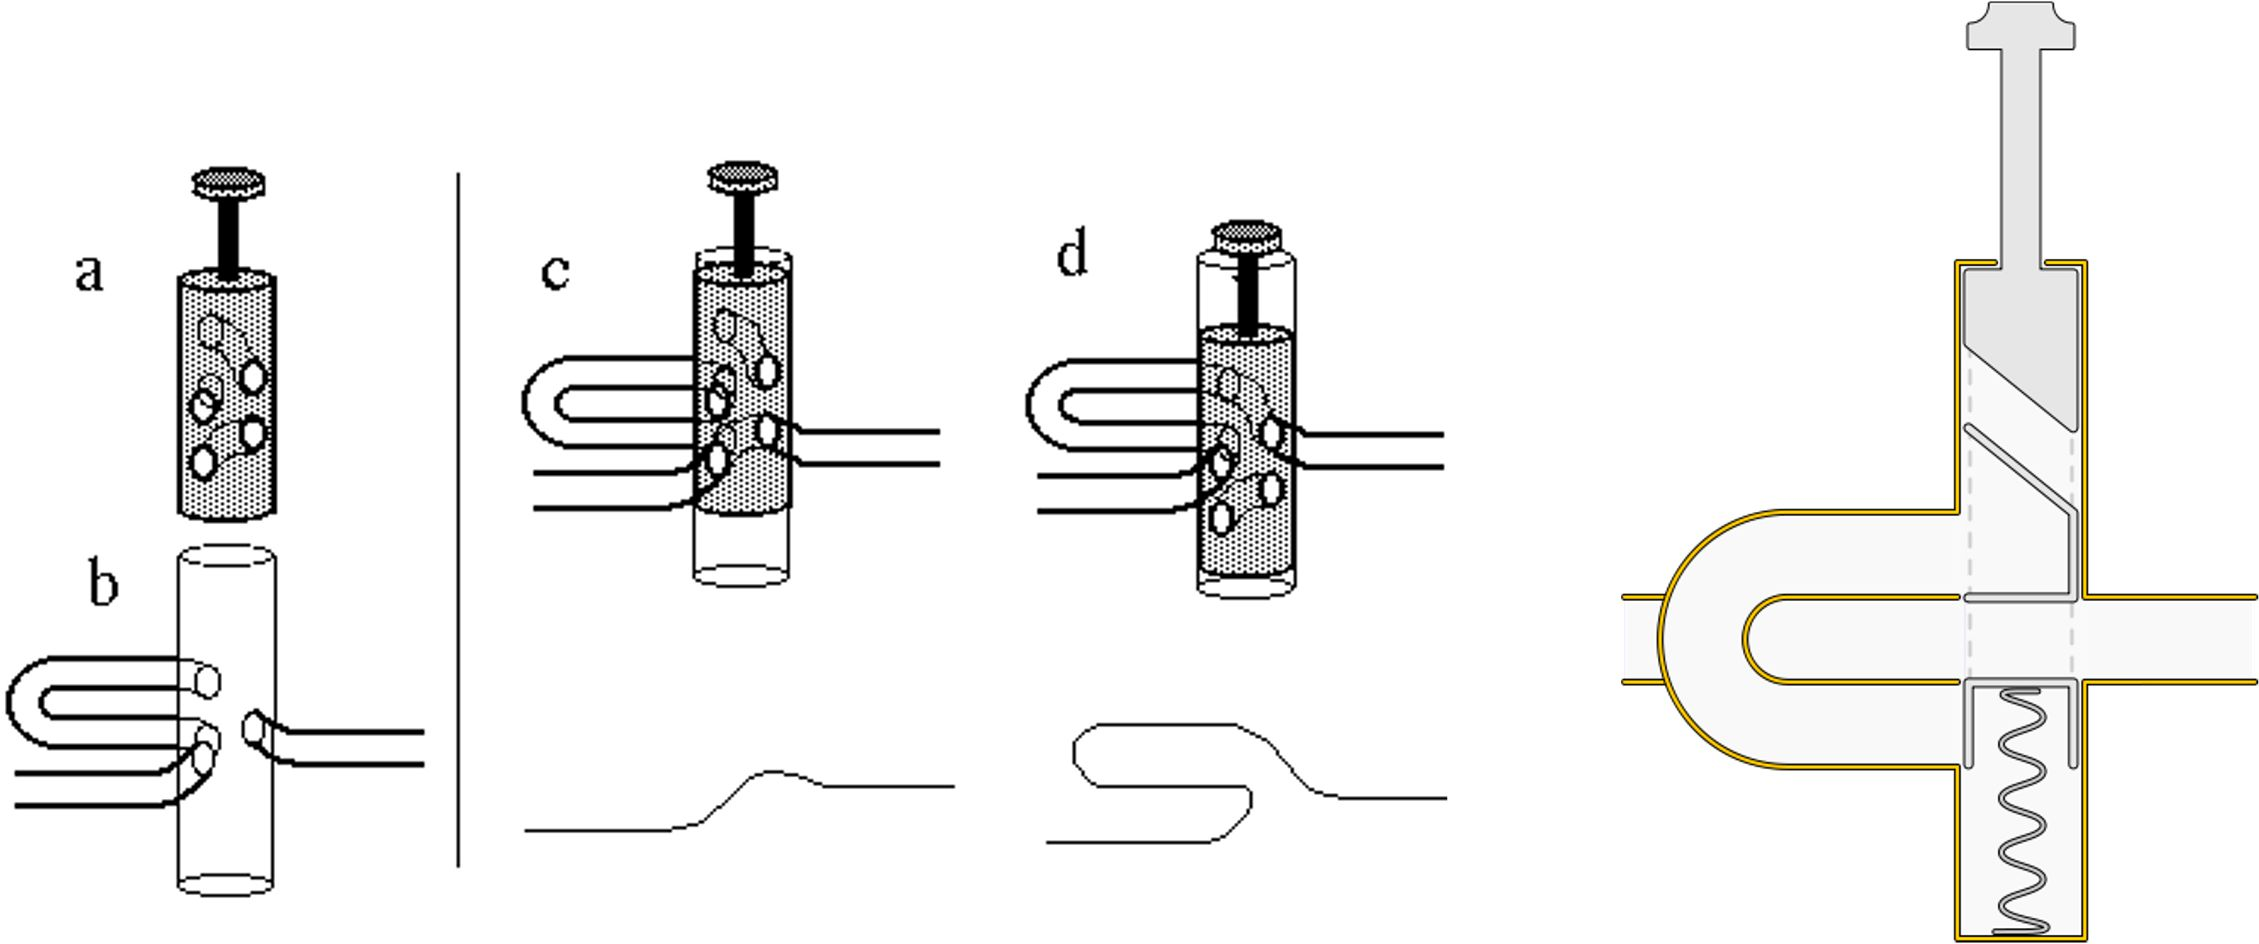
\includegraphics[width=0.7\linewidth]{00_Images/05_chapter/img151.jpg}
\caption{Valve principle and typical configurations}
\label{fig:valves_principle}
\end{figure}

\subsection{Valve Length Increments and Practical Tuning}

An equal-tempered semitone corresponds to a frequency change of about \( 6\% \). Therefore, to lower the frequency of a note by one semitone, the tube length must be increased by roughly a factor \( 1.06 \). If the required length extension for one semitone is written as \( 1 + x \), then a shift of \( n \) semitones requires
\[
(1 + x)^{n}
\]
which is larger than the linear increase \( 1 + nx \) obtained by combining \( n \) identical valves. This creates a tuning compromise for the usual \( 1 \), \( 2 \), and \( 3 \) semitone valves. 

\begin{itemize}
    \item If the three valves are tuned so that the total length equals \( (1 + x)^{n} \) when combined, then the individual semitone shifts become too sharp.
    \item If the valves are tuned so that each one individually produces exactly \( 1 \), \( 2 \), and \( 3 \) semitones, respectively, then pressing all three produces a total tube length that is too long, making the combined shift flat.
    \item A practical compromise is used: for instance, valve 3 may be tuned flat and valves \( 1+2 \) are used for the 3-semitone shift, while valve 3 is reserved for 4, 5, and 6 semitone shifts when combined with valve 1, valve 2, or both. 
\end{itemize}

Practical length increments required for pitch changes are summarized in figure \ref{fig:slide_extension_semitones}.

\begin{figure}[!htb]
\centering
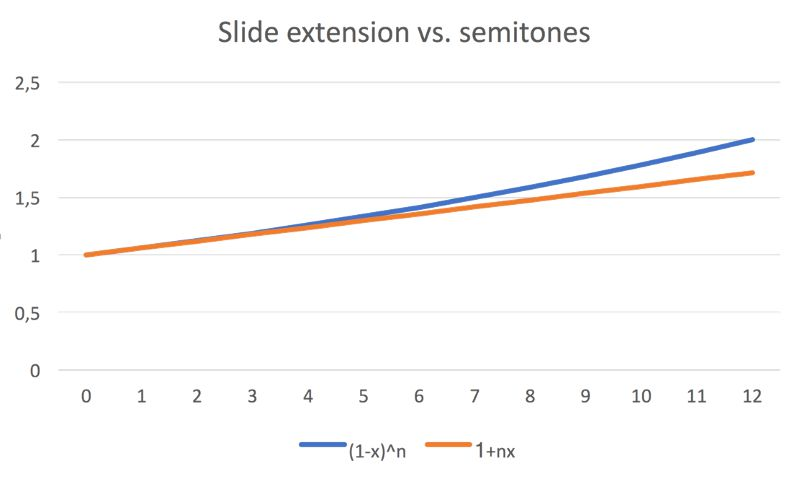
\includegraphics[width=0.7\linewidth]{00_Images/05_chapter/img157.jpg}
\caption{Slide extension (or added length) versus pitch change in semitones}
\label{fig:slide_extension_semitones}
\end{figure}

\section{Excitation and Nonlinearities}

\subsection{Small Amplitude Nonlinearities}

The small-amplitude description applies to gently blown notes. As discussed for reed- and lip-driven generators, the relation between acoustic volume flow and pressure is nonlinear. A convenient representation is a power-series expansion
\[
U = a_{1}p + a_{2}p^{2} + a_{3}p^{3}
\]
where the coefficients \( a_{n} \) are frequency dependent and may also encode a phase shift. Since the pressure is periodic, it can be written as a Fourier series
\[
p = \sum_{n} p_{n}\cos(n\omega t + \phi_{n})
\]
Consider a single flow component \( U \). The \( m \)-th order term in the nonlinear flow relation generates products of harmonics, leading to contributions of the form
\[
p_{i}p_{j}\cdots p_{k}\cos\left[(i \pm j \pm \cdots \pm k)\omega t + (\phi_{i} \pm \phi_{j} \pm \cdots \pm \phi_{k})\right]
\]
Collecting all terms at frequency \( n\omega \), one obtains an expression of the form
\[
U_{n}
= a_{n1}p_{n}
+ \sum_{k} a_{n2}p_{n\pm k}p_{k}
+ \sum_{j,k} a_{n3}p_{n\pm j\pm k}p_{j}p_{k}
+ \cdots
\]
showing explicitly how nonlinearities couple harmonic components. The lip generator is coupled to an instrument with input impedance \( Z(\omega) \). At the throat, the harmonic components satisfy
\[
p_{n} = Z_{n}U_{n}
\]
If only the fundamental is retained and terms above the third order are neglected, the governing relation can be reduced to:
\[
Z_{1}^{-1}p_{1} = a_{11}p_{1} + a_{13}p_{1}^{3}
\]
which yields the amplitude estimate
\[
p_{1} \approx \left[\frac{a_{11} - Z_{1}^{-1}}{-a_{13}}\right]^{1/2}
\]
With \( a_{11} > 0 \), \( a_{13} < 0 \), and \( \Re(Z_{1}) > 0 \), the fundamental pressure reaches its maximum when the instrument input impedance is maximal. The same conclusion applies to the first harmonic, whose pressure is maximized near an impedance maximum at \( 2\omega \).

\subsection{Large Amplitude Nonlinearity}

As the oscillation amplitude increases with blowing pressure, solving the coupled equations for pressure and flow becomes progressively more difficult, and determining the coefficients \( a_{nj} \) in the series description is no longer practical. At the same time, interactions among harmonics and harmonically driven pipe modes become stronger as higher harmonics grow. A more physical viewpoint is therefore required.  Representative large-amplitude waveforms of pressure and volume flow are shown in figure \ref{fig:brass_waveforms_pressure_flow}.

\begin{figure}[!htb]
\centering
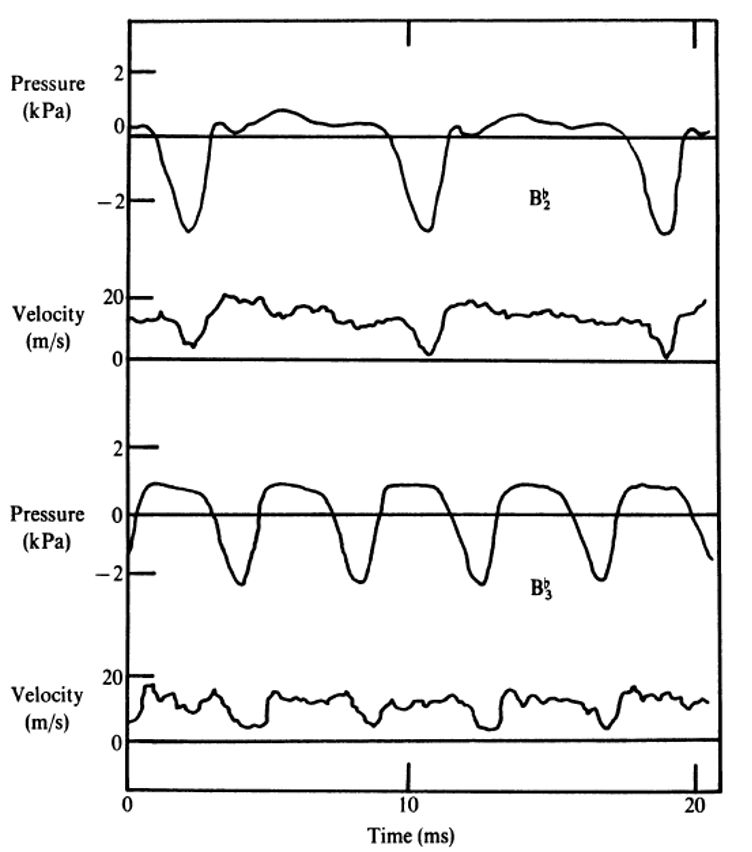
\includegraphics[width=0.7\linewidth]{00_Images/05_chapter/img165.jpg}
\caption{Large-amplitude pressure and volume-flow waveforms in a brass instrument}
\label{fig:brass_waveforms_pressure_flow}
\end{figure}

\paragraph{Pressure and Flow Waveforms}

Measurements of mouth-cup pressure and flow velocity for played trombone notes illustrate that, at high excitation, both waveforms can become strongly non-sinusoidal and noticeably asymmetric over the cycle. A simplified nonlinear relation between volume flow and mouthpiece pressure can be written as
\[
U = \gamma x(p_{0} - p)^{1/2}
\]
where \( x \) is the lip opening and \( \gamma \) is a constant. If the instrument is played at a resonance, it can be approximated by a simple acoustic resistance \( R \), so that \( p \approx UR \). Combining the two relations yields
\[
U \approx \frac{R\gamma^{2}x^{2}}{2}
\left[\left(1 + \frac{4p_{0}}{R^{2}\gamma^{2}x^{2}}\right)^{1/2} - 1\right]
\]

\paragraph{Approximations} Two limiting cases are useful:

\begin{itemize}
    \item If the lip opening is small and the blowing pressure is large, so that \( 4p_{0} \gg R^{2}\gamma^{2}x^{2} \), then
    \[
    U \approx \gamma x p_{0}^{1/2}
    \]
    \item If the lip opening is large and the blowing pressure is moderate, so that \( 4p_{0} \ll R^{2}\gamma^{2}x^{2} \), a second-order expansion gives
    \[
    U \approx \frac{p_{0}}{R} - \frac{p_{0}^{2}}{R^{3}\gamma^{2}x^{2}}
    \]
\end{itemize}

\paragraph{Time Dependent Behavior} Assume the effective lip opening follows an approximately sinusoidal motion,
\[
\gamma x \approx a_{0} + a\sin(\omega t)
\]
In the small-excitation limit,
\[
U \approx a_{0}p_{0}^{1/2} + ap_{0}^{1/2}\sin(\omega t)
\]
and the mouthpiece pressure is approximately \( R \) times this quantity. In the large-excitation case,
\[
U \approx \frac{p_{0}}{R} - \frac{p_{0}^{2}}{R^{3}(a_{0} + a\sin(\omega t))^{2}}
\]
If the lips close just once per cycle, one has \( a \approx a_{0} \), and the second term introduces a strongly distorted component. When \( \sin(\omega t) > 0 \), the correction is small and \( U \) saturates toward \( p_{0}/R \). When \( \sin(\omega t) = -1 \), the correction becomes large and negative and \( U \) drops well below zero. 

\paragraph{Final Considerations} In this simplified picture, the acoustic volume flow oscillates between extremes
\[
\frac{p_{0}}{R}
\qquad
-\frac{p_{0}^{2}}{R^{3}}
\]
leading to asymmetrical flow and pressure waveforms with a negative offset. Once the mouth cup flow waveform is known, it can be used as an input to the instrument impedance in order to determine the acoustic pressure in the mouth cup. At very high playing levels, further effects become relevant. The sound pressure level in the mouthpiece can reach about \SI{175}{\decibel}. At such levels, the wave equation becomes nonlinear, and in long bores, such as trumpets and trombones, shock waves can be produced.

\section{Spectral Features and Mutes}

\subsection{Spectral Features}

Both steady-state and transient properties of brass-instrument spectra can be summarized through a small set of robust trends.

\begin{itemize}
    \item The attack transient typically lasts \( 50 \pm \SI{20}{\milli\second} \), and this duration is approximately independent of the played note and the instrument. 
    \item The steady-state spectral envelope is characterized by a cutoff frequency: below the cutoff, radiated spectral components are roughly equal in amplitude or rise gradually with frequency, while above the cutoff, the amplitude decreases sharply as the frequency increases. 
    \item Typical slopes are in the range \SIrange{2}{4}{\decibel} per octave below the cutoff and \SIrange{15}{25}{\decibel} per octave above the cutoff.
    \item Playing more loudly shifts a larger fraction of radiated power into partials near and above the cutoff. Correspondingly, the slope below the cutoff increases and the slope above the cutoff decreases as intensity increases. 
    \item The cutoff frequency occurs in a comparable part of the frequency range for different instruments, so that spectral envelopes can be scaled and meaningfully superimposed. 
\end{itemize}

The comparison plot illustrates this scaling idea by showing that the mid-frequency envelopes of the trumpet, trombone, and tuba can be brought into close correspondence once the frequency axis is normalized appropriately, while retaining instrument-dependent deviations in level. 

\subsection{Mutes}

Mutes are especially effective in brass instruments because the radiation is dominated by the horn mouth, so the radiated sound can be altered in a controlled and repeatable way. A mute reduces the sound level, but the reduction is generally frequency dependent, so timbre is also modified. Different mute designs exploit this frequency dependence to produce characteristic tone colors. Two broad fitting strategies are commonly distinguished. Open mutes fit tightly in the instrument bell, while closed mutes are supported on cork pads, leaving an annular opening. Common mute types and their basic designs are summarized in figure \ref{fig:mute_types}.

\begin{figure}[!htb]
\centering
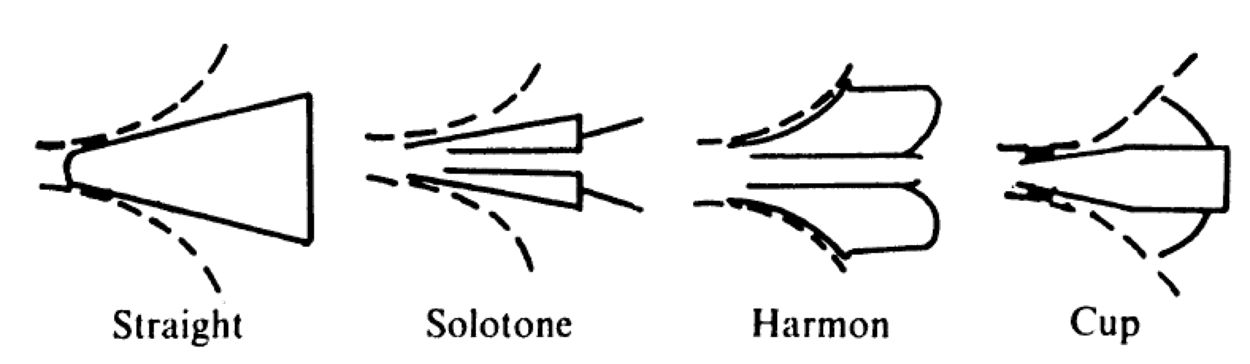
\includegraphics[width=0.7\linewidth]{00_Images/05_chapter/img183.jpg}
\caption{Examples of common brass mutes}
\label{fig:mute_types}
\end{figure}

\paragraph{Spectral Features} The spectrum plot compares the spectral envelopes of a normal B\( ^{\flat} \) cornet note with the same note played using various mutes. The curves show that different designs reshape the envelope in distinct ways across frequency, producing perceptually different brightness and coloration.

\begin{figure}[!htb]
\centering
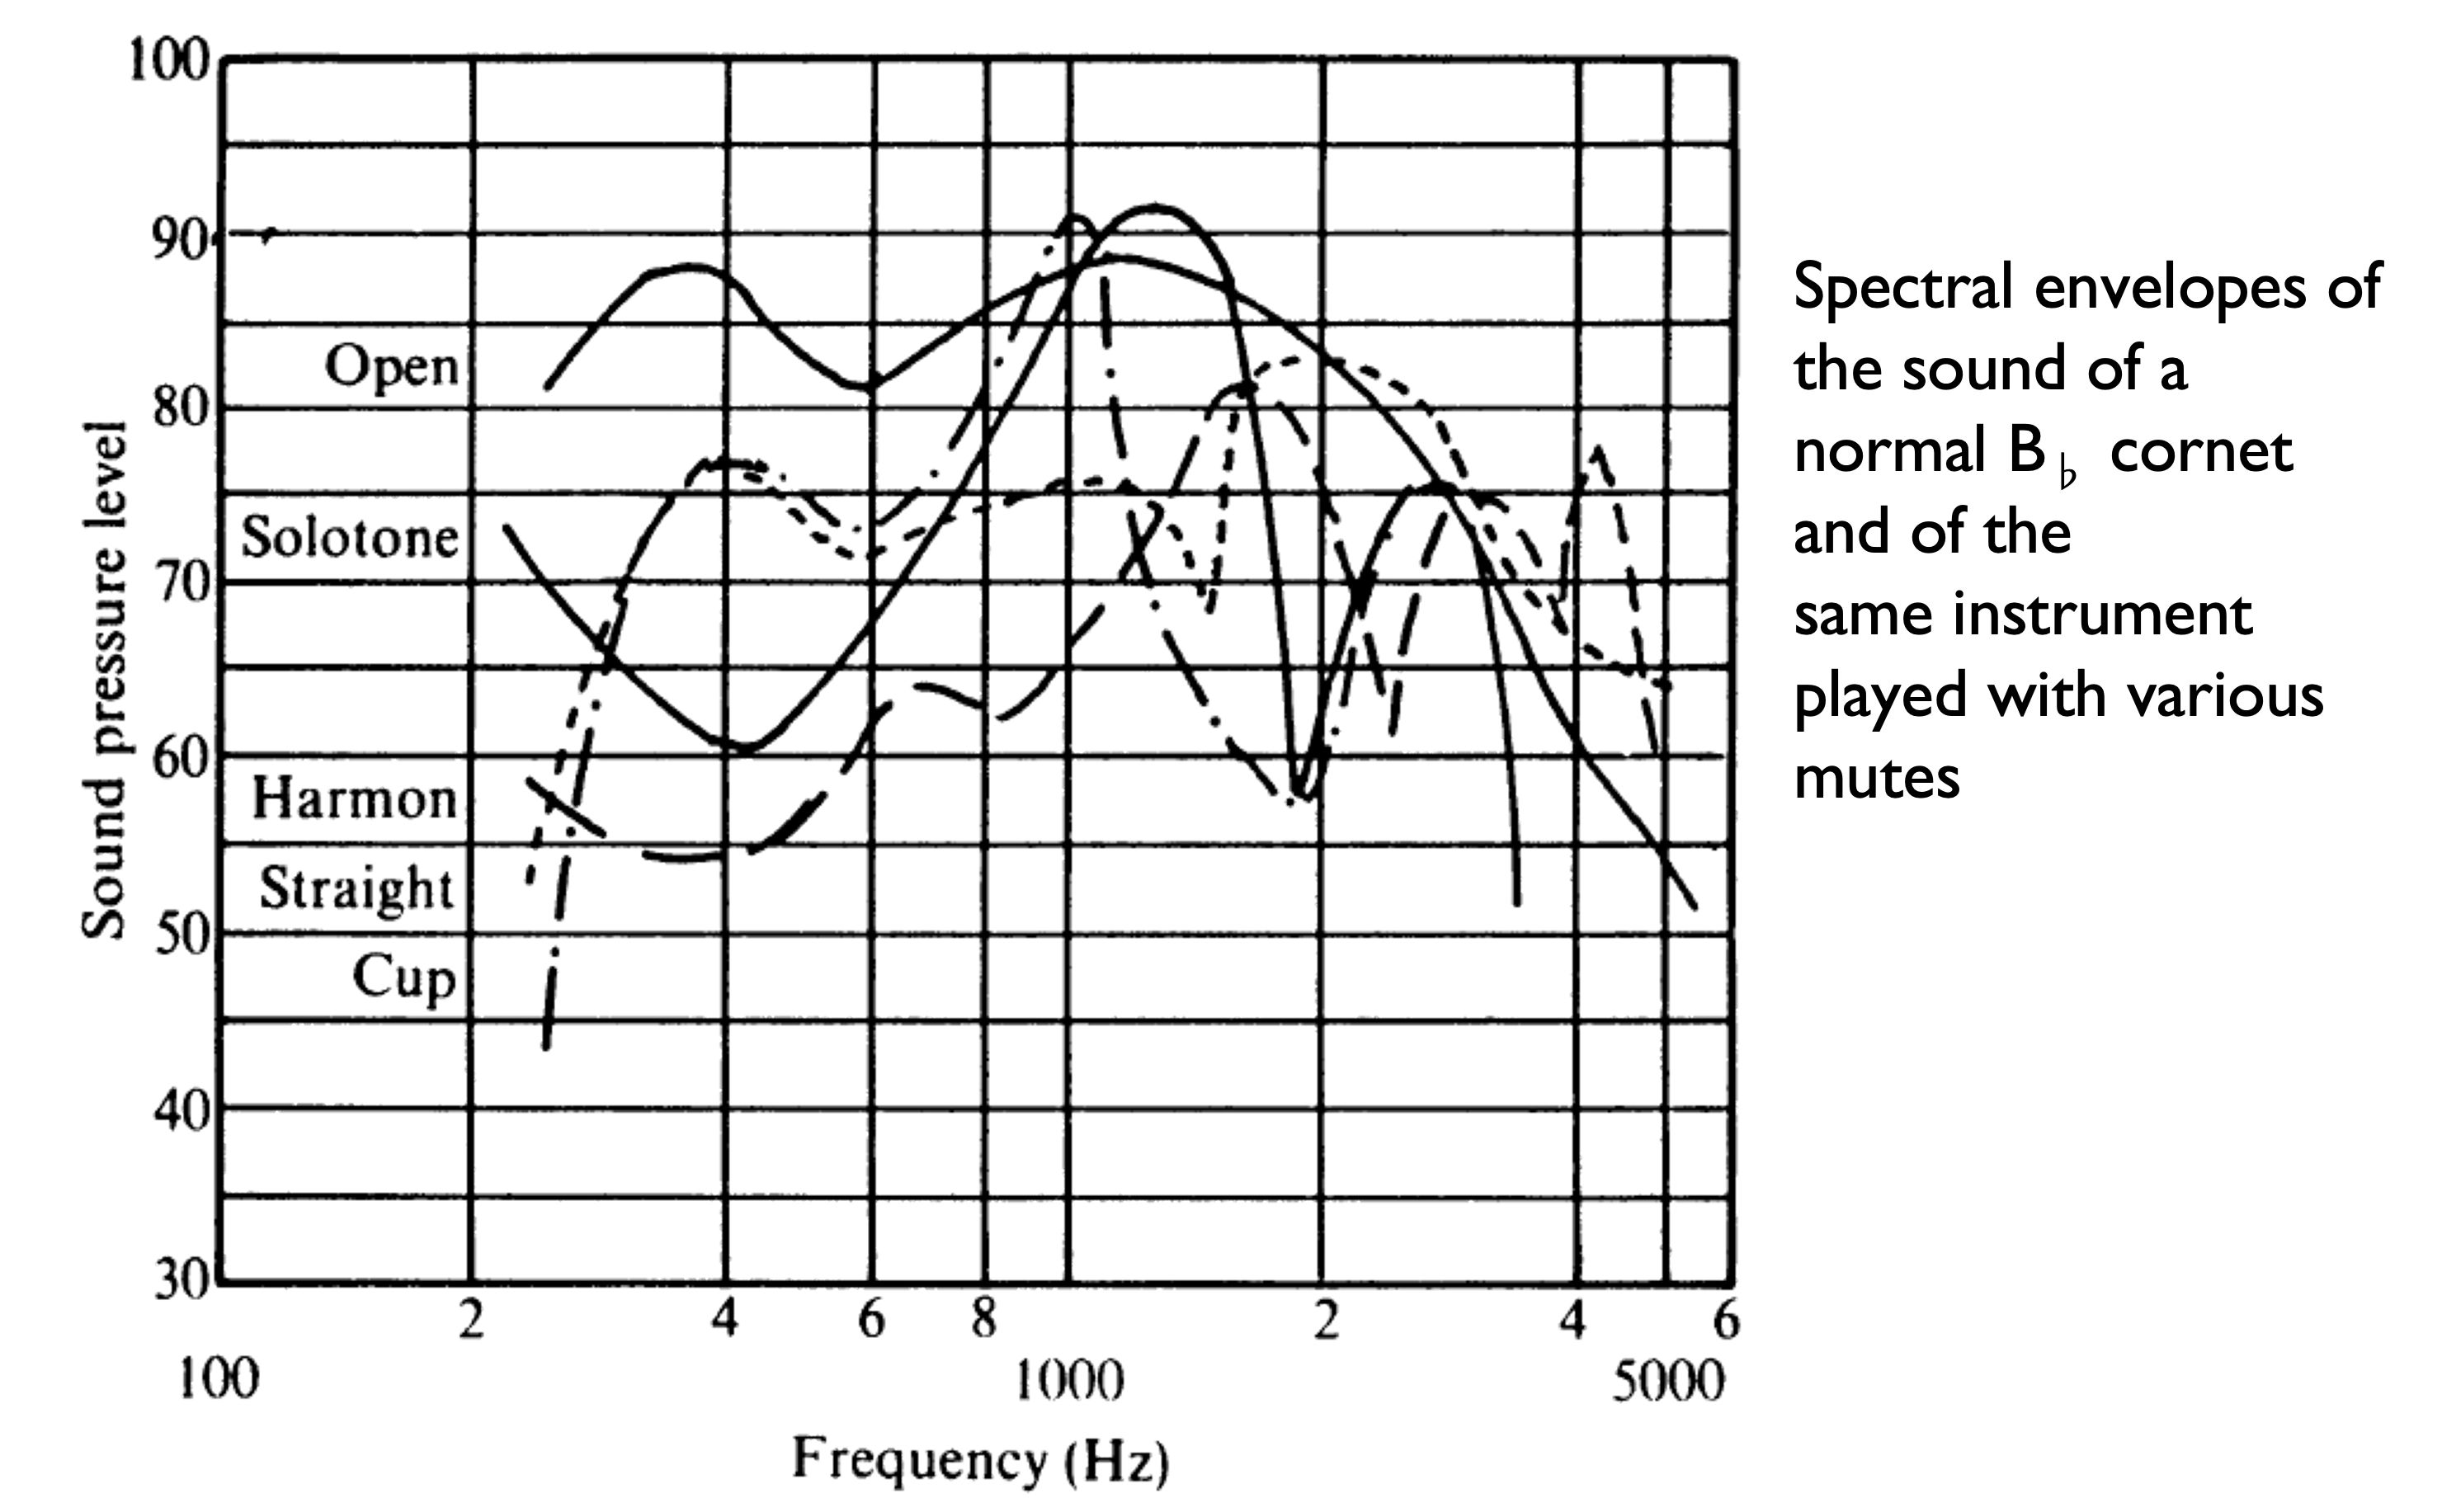
\includegraphics[width=0.7\linewidth]{00_Images/05_chapter/img189.jpg}
\caption{Spectral envelopes with different mutes}
\end{figure}

\paragraph{Considerations} A few recurring acoustic features help to interpret the observed spectral changes.

\begin{itemize}
    \item Most mutes exhibit an admittance maximum, or Helmholtz resonance, associated with their internal cavity, typically in the range \SIrange{200}{300}{\hertz}.
    \item This resonance causes a broad dip in the radiated spectrum around the first and second harmonics over much of the instrument compass, yielding a thinner, reedier, and generally softer sound. 
    \item Additional admittance maxima and minima at higher frequencies are associated with standing waves inside the mute tubes and cavities. 
    \item These higher-frequency resonances and antiresonances lie above about \SI{1000}{\hertz} and contribute strongly to the specific tonal signature of each mute type. 
    \item For some open tube mutes, the radiated sound can be further modified during performance by partially covering the open end with the hand or a cup, producing a wah-wah effect.
\end{itemize}

    %! TEX rootmain.tex

\chapter{Woodwind Instruments}

Woodwind instruments couple a pressure-controlled reed to a resonator whose effective length is adjusted by opening and closing finger holes. The chapter first introduces the bore profiles that best preserve a consistent modal structure under length reduction, then discusses the acoustic role of finger holes and the practical consequences for tuning, temperament, and temperature dependence. Methods for input-impedance computation and for sound radiation are subsequently outlined, and the chapter closes with an overview of common woodwind families, with specific remarks on clarinet, oboe, and saxophone. 

\section{Bore Shapes}

\subsection{Bore Shapes with Finger Holes}

In brass-type instruments nearly the entire horn length, including the flaring bell, is always used as a resonator. For instruments with finger holes the situation is different, because the lower part of the resonator can be partly decoupled by open holes. In this sense, open holes modify the effective acoustic length of the resonator. To preserve a consistent tone quality while the acoustic length is reduced, the resonator should scale as its length changes. A profile that preserves its shape under truncation is described by the power law
\[
S(x) = ax^{\epsilon}
\]
defined for
\[
0 \le x \le L
\]
so that the resonant frequencies \( \omega_n \) scale inversely with the length \( L \). 

\subsection{Power-Law Profiles and Bessel Horns}

For a Bessel horn with parameter \( \epsilon \ge 0 \) extending to \( x = 0 \), the acoustic pressure can be written as
\[
p(x) = Ax^{(1-\epsilon)/2}J_{-(1-\epsilon)/2}(kx)
\]
where \( J_{\nu} \) is a Bessel function of order \( \nu \) and
\[
k = \frac{\omega}{c}
\]
Assuming the bore is essentially open at \( x = L \) and neglecting radiation impedance (ideal open-end condition; radiation reactance can be included via an end correction, and radiation losses affect resonance widths), the normal modes occur at angular frequencies \( \omega_n \) given by the roots of
\[
J_{-(1-\epsilon)/2}\left(\frac{\omega L}{c}\right) = 0
\]
This shows that, when \( \epsilon > 0 \), the mode frequencies \( \omega_n \) scale inversely with \( L \), and that no other horn shape has this property. 

\subsection{Musically Useful Bore Profiles}

The mode frequencies derived from the Bessel condition correspond to input-impedance maxima at the mouthpiece, consistent with driving by a pressure-controlled reed. Based on the root structure of Bessel functions, three candidates are highlighted as musically useful approximations:

\begin{itemize}
    \item \( \epsilon = 0 \) (cylindrical bore), associated with an odd-harmonic series \( 1,3,5,\ldots \)
    \item \( \epsilon = 2 \) (conical bore), associated with a complete harmonic series \( 1,2,3,\ldots \)
    \item \( \epsilon \) slightly larger than \( 7 \), yielding a series close to \( 1,(1!),2,(2!),3,\ldots \), though the large flare rate raises practical difficulties
\end{itemize}

As a consequence, useful bore profiles for reed- or lip-driven instruments using finger holes should approximate cylinders or cones fairly closely. In lip-driven instruments with finger holes (e.g. cornet, serpent), the bore is conical, which supports a complete harmonic series and a true fundamental. Reed-driven woodwinds can be either cylindrical or conical.

\subsection{Input Impedance Review: Cylinder and Cone}

For a cylindrical tube of length \( L \) and cross-sectional area \( S = \pi a^2 \), open at its far end, the input impedance can be approximated as
\[
Z_{\mathrm{in}} \approx jZ_{0}\tan(kL')
\qquad
Z_{0} = \frac{\rho c}{S}
\qquad
L' = L + 0.6a
\]
with impedance maxima at
\[
\omega_n = \left(n - \frac{1}{2}\right)\frac{\pi c}{L'}
\]
For a cone of geometrical length \( L \), with throat area \( S_1 \) at a distance \( x_1 \) from the conical vertex and open at the mouth, the input impedance can be written as
\[
Z_{\mathrm{in}} \approx
jZ_{1}\frac{\sin(kL')}{\sin(k\theta_{1})\sin(k(L' + \theta_{1}))}
\qquad
Z_{1} = \frac{\rho c}{S_{1}}
\]
with
\[
k\theta_{1} = \tan^{-1}(kx_{1})
\qquad
L' = L + 0.6a
\]
Under the hypotheses \( x_{1} \ll L \) and \( \theta_{1} \approx x_{1} \), the modal frequencies become
\[
\omega_n = \frac{n\pi c}{L' + x_{1}}
\]
forming a complete harmonic series. 

\subsection{Cylindrical Versus Conical Bores}

To obtain harmonic behavior, woodwind bores must be close to conical (\( \epsilon = 2 \)) or cylindrical (\( \epsilon = 0 \)). For a cylindrical instrument,
\[
\omega_n = \left(n - \frac{1}{2}\right)\frac{\pi c}{L'}
\]
so the resonance series follows odd harmonics. For a conical instrument,
\[
\omega_n = \frac{n\pi c}{L' + x_{1}}
\]
so the resonance series is fully harmonic. For the same geometrical length \( L \), the fundamental frequency of a cylindrical instrument is about half that of a conical instrument. Typical conical bass instruments (e.g. bassoons) therefore use long pipes, often folded to remain practical in size. 

\begin{table}[!htb]
\centering
\begin{tabular}{lcccccc}
\hline
Instrument  & Musical Range     & Tube Length   & Top Diameter  & Bell Diameter             & Semi-Angle        \\
\hline
Clarinet    & D3--G6            & 664           & 14            & \(16 \rightarrow 60\)     & \(0^{\circ}\)     \\
Oboe        & B\(\flat\)3--G6   & 644           & 3             & \(13 \rightarrow 37\)     & \(0.7^{\circ}\)   \\
Bassoon     & B\(\flat\)1--C5   & 2560          & 4             & 40                        & \(0.4^{\circ}\)   \\
Alto Sax    & D3--A6            & 1062          & 12            & \(70 \rightarrow 123\)    & \(1.6^{\circ}\)   \\
\hline
\end{tabular}
\caption{Representative Bore Dimensions Of Common Woodwinds (Dimensions In Millimetres)}
\end{table}

\section{Finger Holes}

Finger holes change the effective length of the air column, enabling the production of different notes. Early instruments were typically limited to fixed 7-note or 5-note scales, with a small number of holes of simple geometry. Modern instruments support chromatic and extended scales, and use key mechanisms to operate combinations of holes reliably. 

\subsection{Tone Control Through Finger Holes}

Consider a cylindrical tube with one finger hole at a small distance \( D \) from the open end. The open hole has a chimney of height \( l \). The analysis assumes that both \( l \) and \( D \) are small with respect to the wavelength. For a cylindrical pipe of acoustic length \( L' \), the input impedance can be written as
\[
Z = jZ_0 \tan(kL')
\qquad
Z_0 = \frac{\rho c}{S}
\]
where the acoustic length includes the standard open-end correction
\[
L' \approx L + 0.6a
\]
with \( a \) the pipe radius. When the hole is open, the portion of tube from the hole to the open end modifies the overall impedance as if there were an effective change in length. At the position of the hole, the admittance presented to the upstream pipe is the parallel combination
\[
Y = Y_{\mathrm{hole}} + Y_{\mathrm{pipe}}
= -j\frac{S_1}{\rho c}\cot(kl) - j\frac{S}{\rho c}\cot\left(k(D+\Delta)\right)
\]
where \( S_1 \) is the hole cross-sectional area and \( \Delta \) is the end correction at the open end of the main pipe. If \( l \) and \( D \) are small compared to the wavelength, using the first-order approximation \( \cot(x) \approx 1/x \) gives
\[
Y \approx -\frac{j}{\rho\omega}
\left(
\frac{S_1}{l} + \frac{S}{D+\Delta}
\right)
\]
which can be equivalently expressed as
\[
Z \approx j\rho\omega
\left[
\frac{l(D+\Delta)}{S_1(D+\Delta) + Sl}
\right]
\]
A simple continuation of the acoustic tube past the hole position by an amount \( \Delta' \) would present an impedance
\[
Z \approx \frac{j\rho\omega \Delta'}{S}
\]
so that the effective end correction at the hole position is
\[
\Delta' \approx \frac{Sl(D+\Delta)}{S_1(D+\Delta) + Sl}
\]
The acoustic length of the tube with its open hole is therefore reduced below that of the original tube by
\[
\delta = D + \Delta - \Delta'
= \frac{S_1(D+\Delta)^2}{S_1(D+\Delta) + Sl}
\]
In the special case \( S_1 = S \) and \( l \approx \Delta \), the reduction becomes approximately
\[
\delta \approx D + \frac{\Delta^2}{D + 2\Delta}
\]

\paragraph{Considerations} For smaller finger holes, the acoustic-length reduction is considerably less than \( D \). A reduction in \( S_1 \) can be compensated by increasing the distance \( D \) from the open end, implying greater separation between adjacent holes. At higher frequencies, when \( D \) is no longer small compared to the wavelength, the preceding low-frequency approximations no longer hold.

\subsection{Finger Holes Positioning in the Lower Register}

In the lower register of a cylindrical wind instrument, a practical guideline is:

\begin{enumerate}
    \item Start from the hole farthest from the mouthpiece (the instrument foot).
    \item Choose \( S_1 \) and \( D \) so that the pipe undergoes an acoustic-length decrease of \( \SI{12}{\percent} \) (whole tone) or \( \SI{6}{\percent} \) (semitone).
    \item Repeat the same procedure starting from the new acoustic length for the next hole, and so on.
\end{enumerate}

In real instruments, hole placement is more complicated, and must also account for deviations from ideal harmonic relationships caused by the holes themselves, together with constraints on playing comfort.

\subsection{Fingering Systems}

Most wind instruments adopt a fingering system based on a preset configuration. The left hand is placed close to the mouthpiece, and the left thumb supports the instrument from below. Three fingers (excluding thumb and little finger) are used to operate the main finger holes, while other fingers manipulate keys for register changes or for accessing very low or very high notes. The left- and right-hand configuration determines the note produced, and real systems refine this baseline by adding holes and keys that extend the playable range.

\section{Tuning, Temperament, Temperature}

\subsection{Reference Pitch}

A practical reference for orchestral tuning is the standard pitch
\[
A_4 = \SI{440}{\hertz}
\]
which is set by international agreement. Historically, lower references were common, around
\[
A_4 = \SI{435}{\hertz}
\]
while military wind bands in the last century sometimes adopted a pitch nearly one semitone higher. Some major orchestras still tune to
\[
A_4 = \SI{442}{\hertz}
\]
often motivated by a perceived increase in brilliance. In orchestral practice the reference note is typically given by the oboe, not because its pitch is intrinsically stable, but because of its characteristic tone quality. 
\subsection{Tuning Issues Across Registers}

Woodwinds exhibit several tuning difficulties that emerge when one attempts to align the instrument to a single reference. 

\begin{itemize}
    \item If the instrument is tuned to the lowest note and then flattened by half a semitone by lengthening the bore at the reed end by about \( \SI{3}{\percent} \), this lengthening corresponds to about \( \SI{6}{\percent} \) for the top note of the register in an oboe and about \( \SI{9}{\percent} \) in a clarinet.
    \item Going from the top note of the lower register to the first note of the second register can produce an extra half semitone in the oboe and a whole semitone in the clarinet. 
    \item Although skilled players can adjust pitch to some extent, such register jumps are too large to be handled comfortably by embouchure control alone.
\end{itemize}

Historical and practical design responses have been adopted to mitigate these issues. 

\begin{itemize}
    \item In the 18th century, some woodwinds were supplied with two different middle joints to help manage register alignment. 
    \item Modern bassoons are commonly supplied with at least two bocals (crooks) of different taper, providing alternative tuning compromises.
\end{itemize}

\subsection{Temperature Effects And Thermal Gradients}

Since the speed of sound increases with temperature, a cold woodwind tends to play flat and its pitch rises as the instrument warms up. This drift is unfortunate in ensemble contexts because it occurs in the opposite direction to the typical drift of string instruments. A further complication is that warming is generally uneven along the bore. 

\begin{itemize}
    \item The upper bore near the reed tends to reach a higher temperature than the lower bore, and the resulting gradient varies with room temperature. 
    \item If the reed end is at about \SI{35}{\celsius} and the lower end at about \SI{20}{\celsius}, the difference in absolute temperature is about \( \SI{5}{\percent} \) and the corresponding difference in sound speed about \( \SI{2.5}{\percent} \).
    \item Averaged over the bore length, this can make notes with nearly all finger holes closed flat with respect to notes with nearly all holes open by as much as \( \SI{1}{\percent} \), i.e. about one sixth of a semitone.
\end{itemize}

As a consequence, woodwind players cannot treat pitch and temperament as fixed, but must rely on auditory feedback and subtle real-time adjustments during performance.

\section{Impedance Computation}

A first-order description of woodwind acoustics is sufficient to estimate an acoustic length and the resonance frequency of the first one or two modes, but it is not enough to predict real playing conditions. A complete input-impedance curve as a function of frequency is needed at a convenient reference point close to the reed. In this view, the acoustic behavior of a real instrument is characterized by the impedance curve near the reed together with the nonlinear behavior of the reed valve. Two complementary approaches are commonly adopted: measurement-based impedance estimation and numerical impedance computation.

\subsection{Computation}

In measurement-based estimation, the input impedance is obtained from local pressure and volume flow measurements, through
\[
Z = \frac{p}{U}
\]
which requires appropriate transducers to estimate \( p \) and \( U \) at the chosen reference point. In numerical computation, the bore is subdivided into a sequence of short elements whose shape can be approximated as cylindrical or conical. Each element is treated as a four-terminal (two-port) component relating pressures and volume flows at its ends:
\[
\left\{
\begin{aligned}
p_{1} &= Z_{11}U_{1} + Z_{12}U_{2} \\
p_{2} &= Z_{21}U_{1} + Z_{22}U_{2}
\end{aligned}
\right.
\]
Defining
\[
Z_{1} = \frac{p_{1}}{U_{1}}
\qquad
Z_{2} = \frac{p_{2}}{U_{2}}
\]
and using reciprocity \( Z_{21} = Z_{12} \), the input impedance of the element can be expressed as
\[
Z_{1} = Z_{11} + \frac{Z_{12}^{2}}{Z_{2} - Z_{22}}
\]
so that the impedance of the whole instrument can be assembled by cascading sections from the bell toward the reed.

\subsection{Modeling Finger Holes}

An open or closed finger hole can be represented by a section of zero geometric length, described by the same two-port form and inserted in the bore at the hole location. Different parameter values are used depending on whether the hole is open or closed. For a circular finger hole of radius \( b \) and chimney height \( t \) in a tube of radius \( a \), the equivalent network has a shunt element \( Z_{s} \) and two symmetric series elements \( Z_{a}/2 \). The imaginary parts of these elements can be written as
\[
Z_{s} =
\frac{\rho c}{\pi a^{2}}
\left(\frac{a^{2}}{b^{2}}\right)
\left\{
\begin{aligned}
&-j\cot(kl) &\qquad \text{(closed)} \\
&jk t_{e}   &\qquad \text{(open)}
\end{aligned}
\right.
\]
and
\[
Z_{a} =
\frac{\rho c}{\pi a^{2}}
\left(\frac{a^{2}}{b^{2}}\right)
(-jk t_{a})
\]
where \( t \), \( t_{e} \), and \( t_{a} \) depend on the geometrical and structural details of the finger hole or key hole. A practical tone-hole model and its equivalent network representation are shown in figure \ref{fig:tonehole_model_network}.

\begin{figure}[!htb]
\centering
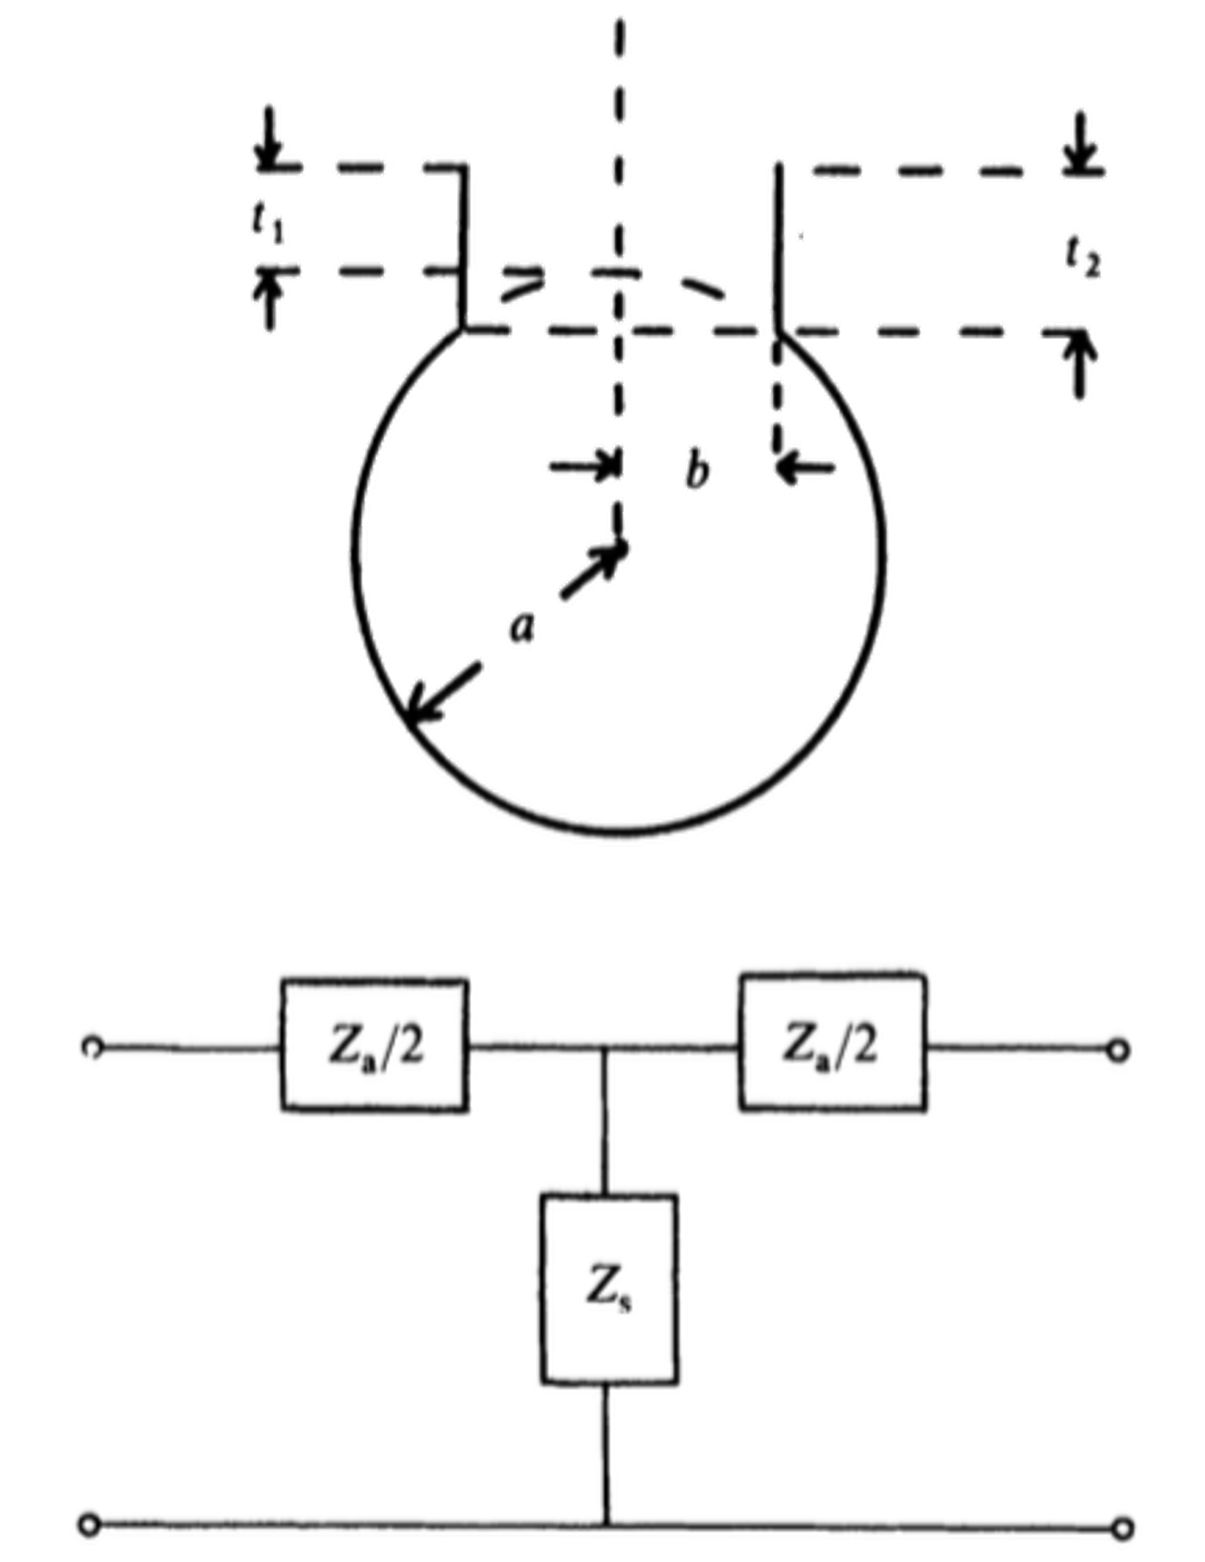
\includegraphics[width=0.7\linewidth]{00_Images/06_chapter/img61.jpg}
\caption{Tone-hole geometry and equivalent network used for impedance computation}
\label{fig:tonehole_model_network}
\end{figure}

\subsection{Impedance Examples}

Measured input-impedance curves illustrate how fingering modifies the resonance pattern.

\paragraph{Clarinet} For a low note and a high note, the frequencies of the fundamental and its harmonics can be marked along the frequency axis. In the higher-note fingering, the first-mode peak is shifted relative to the harmonic grid, indicating that the effective boundary condition created by open holes alters the lowest resonance more strongly than higher ones.

\paragraph{Oboe} For a low note and a high note, the lower impedance peaks exhibit an asymmetric shape, consistent with the influence of a conical bore. In the higher-note fingering, the lower-mode peaks are displaced and reshaped compared to the low-note case.

\section{Sound Radiation}

\subsection{Cutoff Frequency}

The cutoff frequency is the frequency above which sound is radiated freely to the environment without being reflected back into the bore. Above cutoff, the impedance is well coupled to the air characteristic impedance, so pronounced resonances are no longer expected in the radiated spectrum. This aspect contributes strongly to the overall timbre of the instrument. In woodwinds, the cutoff frequency is mostly caused by the presence of finger holes and effectively sets the frequency range over which the instrument behaves as a strongly resonant system. For a pipe of diameter \( 2a \), with holes of diameter \( 2b \) and acoustic length \( l \), separated by \( 2s \), an approximate estimate is
\[
f_c \approx 0.11c\left(\frac{b}{a}\right)\sqrt{\frac{1}{sl}}
\]

\subsection{Sound Radiation Below the Cutoff Frequency}

Sound can radiate from open holes, and the presence of multiple open finger holes makes the radiation pattern complex. The open holes behave like an array of point sources. Below cutoff, several open tone holes can radiate simultaneously; when their phases are similar (typical in the low register), interference leads to a directional pattern that is not purely isotropic, often reduced on-axis and stronger off-axis.

\subsection{Sound Radiation Above the Cutoff Frequency}

Above cutoff, radiation from holes and bell combines. Phase differences between sources produce frequency-dependent lobes and nulls; higher harmonics tend to be more directional, and in practice room reflections partially average these effects.

\subsection{Acoustic Efficiency}

The acoustic output of most woodwind instruments is about \SI{1}{\milli\watt}, corresponding to roughly \SI{80}{\decibel} SPL at \SI{1}{\meter}. The player generates a much greater acoustic pressure than that, on the order of \SIrange{3}{5}{\kilo\pascal}, corresponding to \SIrange{0.3}{0.5}{\watt}. The acoustic efficiency is therefore about \SI{1}{\percent}. The remaining power is mostly absorbed by the reed valve and dissipated by viscous and thermal losses in the pipe.

\subsection{Spectrum Envelope of Reed-Driven Instruments}

The reed strongly influences the radiated sound and can vary greatly with internal nonlinearities, blowing pressure, and playing technique. Tube resonances shape the reed excitation up to the cutoff frequency. Above cutoff, the spectrum exhibits an approximately constant decaying slope of about \SI{-12}{\decibel} for a beating reed and about \SI{-18}{\decibel} for a non-beating reed. An example of how the radiated waveform and spectrum can change with pitch is shown in figure \ref{fig:clarinet_waveform_spectra_example}.

\begin{figure}[!htb]
\centering
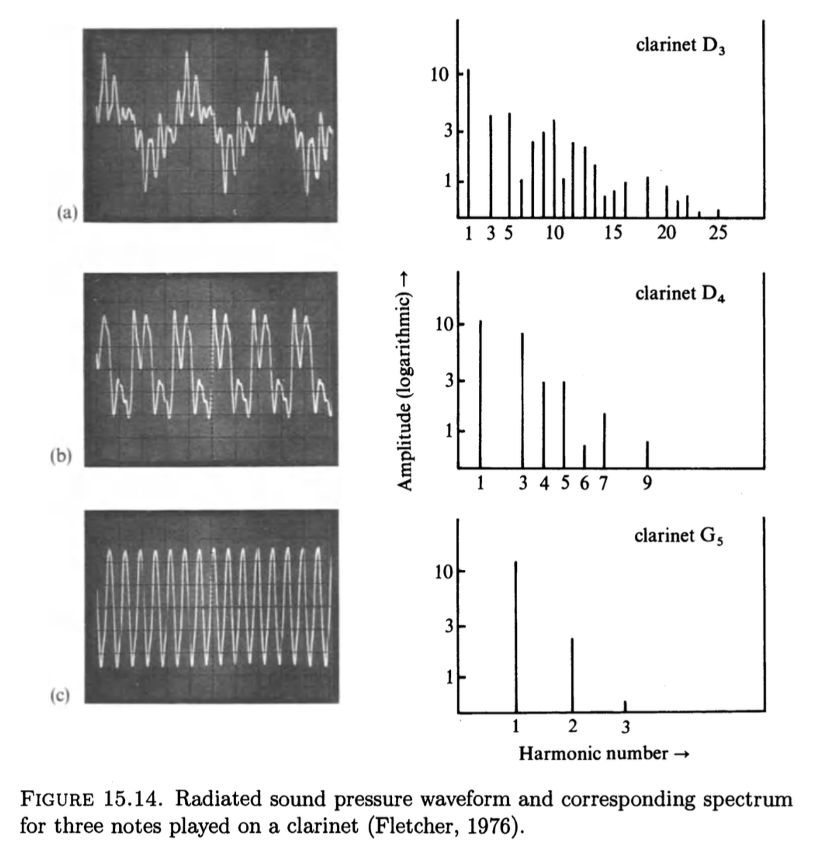
\includegraphics[width=0.7\linewidth]{00_Images/06_chapter/img93.jpg}
\caption{Example of reed-driven waveform and harmonic spectrum across different notes (clarinet)}
\label{fig:clarinet_waveform_spectra_example}
\end{figure}

\section{Woodwind Instrument Overview}

This section summarizes a few representative woodwinds by linking bore geometry, reed type, register mechanism, and spectral features. 

\subsection{Clarinet}

The clarinet is characterized by a cylindrical bore and a single reed. Register changes are achieved through dedicated keys, enabling a wide pitch range: about three octaves organized into two main registers, plus an additional register covering part of the next upper octave. Radiated-pressure waveforms and spectra illustrate how the harmonic content changes across notes, with the low register showing a rich harmonic structure and higher notes exhibiting a different distribution of partials. Representative harmonic spectra for a low and a high clarinet note are shown in figure \ref{fig:clarinet_harmonics_low_high}.

\begin{figure}[!htb]
\centering
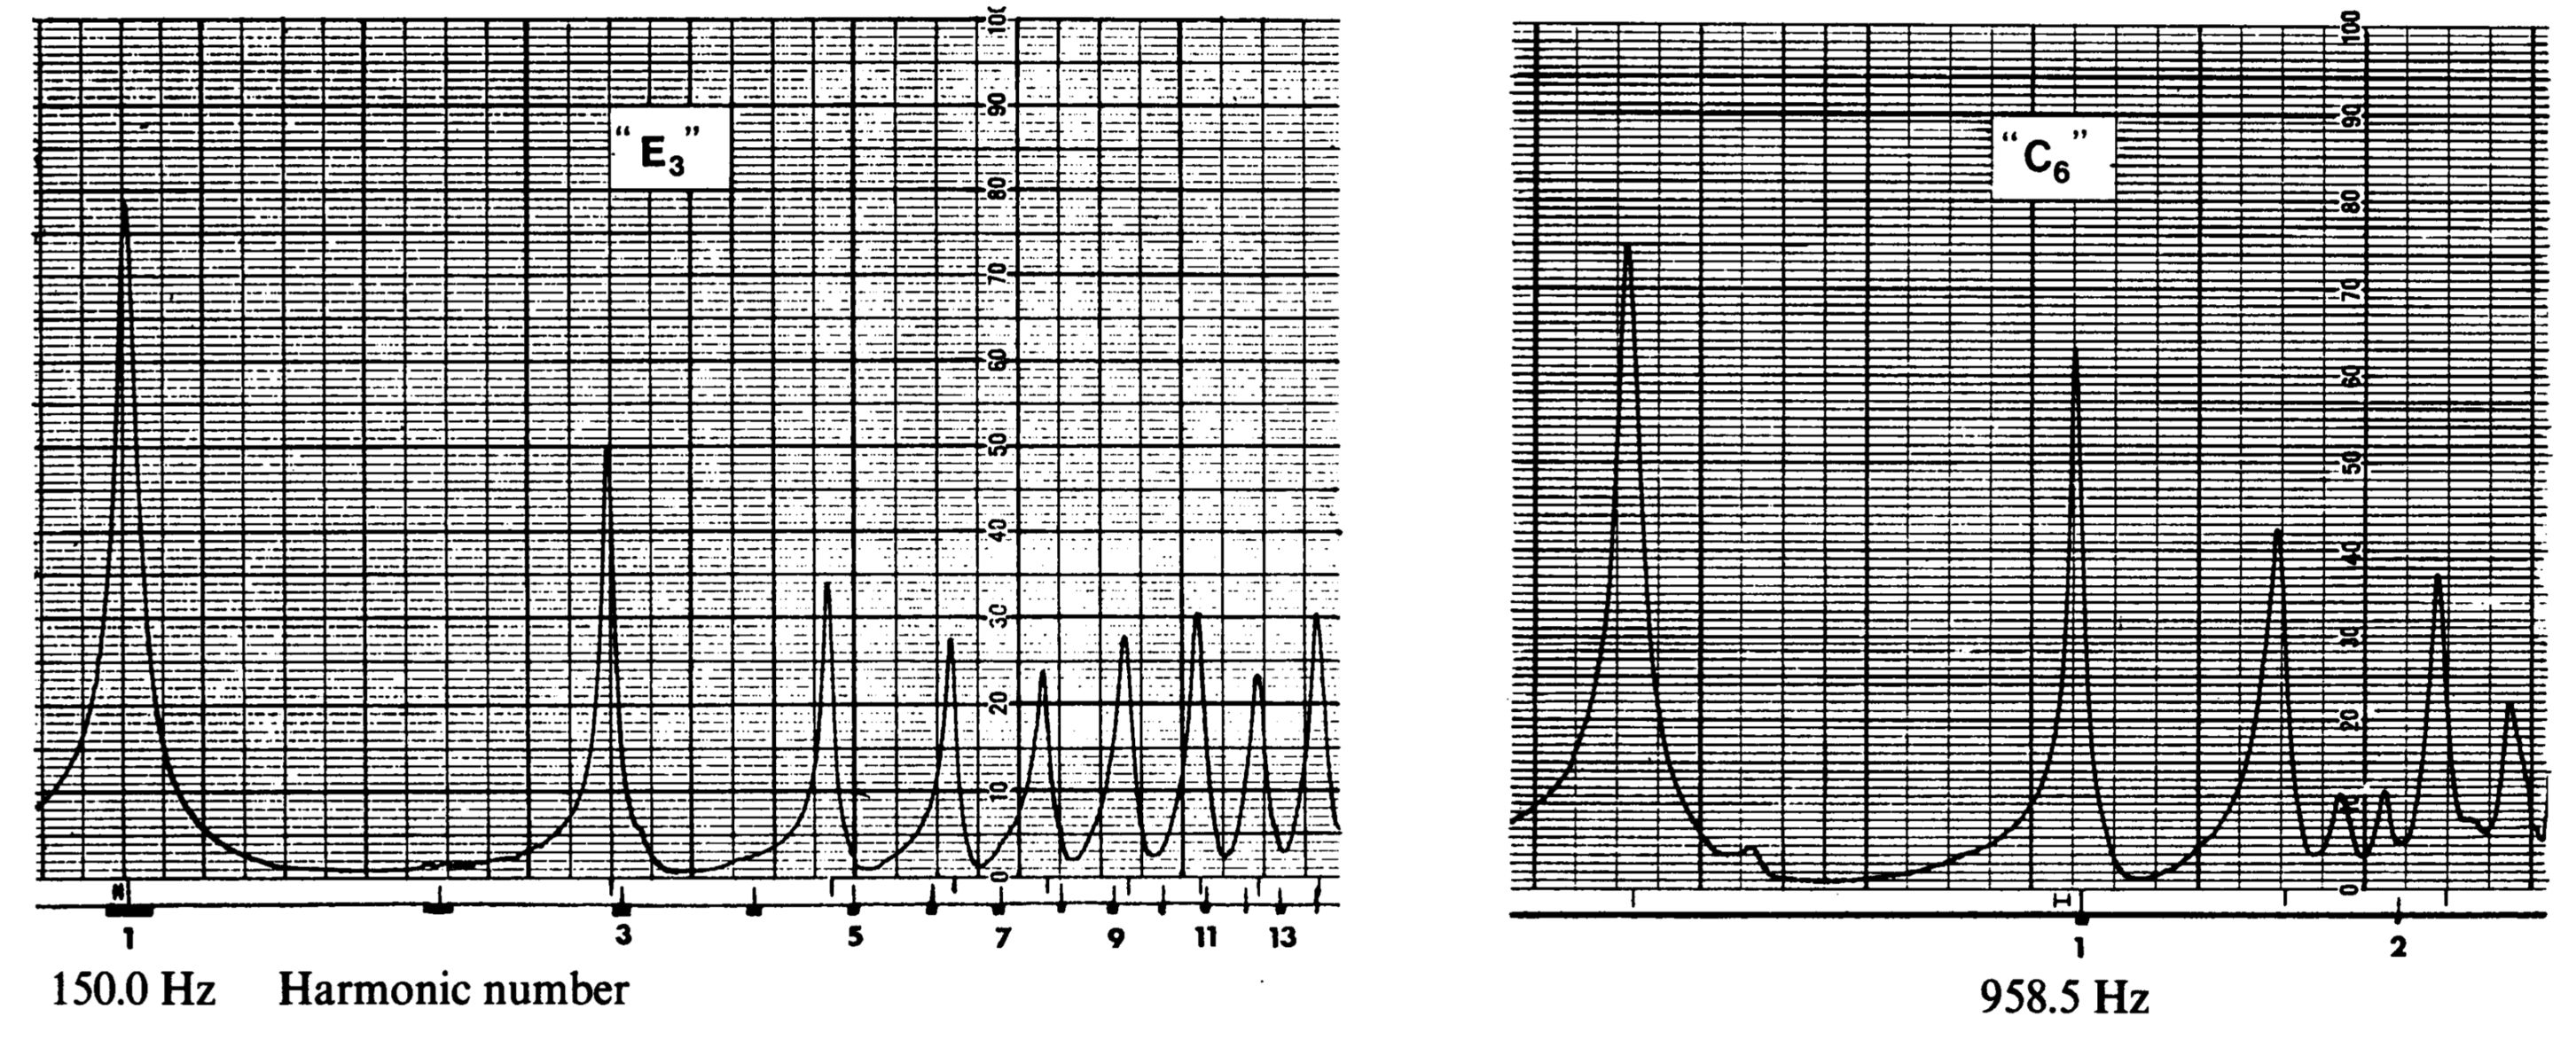
\includegraphics[width=0.7\linewidth]{00_Images/06_chapter/img68.jpg}
\caption{Clarinet harmonic spectra in the low register versus a higher note}
\label{fig:clarinet_harmonics_low_high}
\end{figure}

\subsection{Oboe}

The oboe has approximately the same overall length as the clarinet, but it uses a double reed and a conical bore. A complex keywork allows a large chromatic extension across registers. The conical shape makes the lowest note nearly an octave higher than the clarinet’s lowest note. A relevant playing feature is that the reed always beats, which limits the amount of tone-color variation between soft and loud dynamics compared with non-beating regimes. In spectral terms, lower notes show a strong harmonic spectrum with a comparatively high level of upper harmonics, producing a brighter timbre than the clarinet. The input-impedance peaks and the radiated spectrum initially show peaks rising with frequency, while beyond cutoff the spectrum decreases with a slope of about \SI{-12}{\decibel} per octave, consistent with a beating reed. Representative harmonic spectra for a low and a high oboe note are shown in figure \ref{fig:oboe_harmonics_low_high}.

\begin{figure}[!htb]
\centering
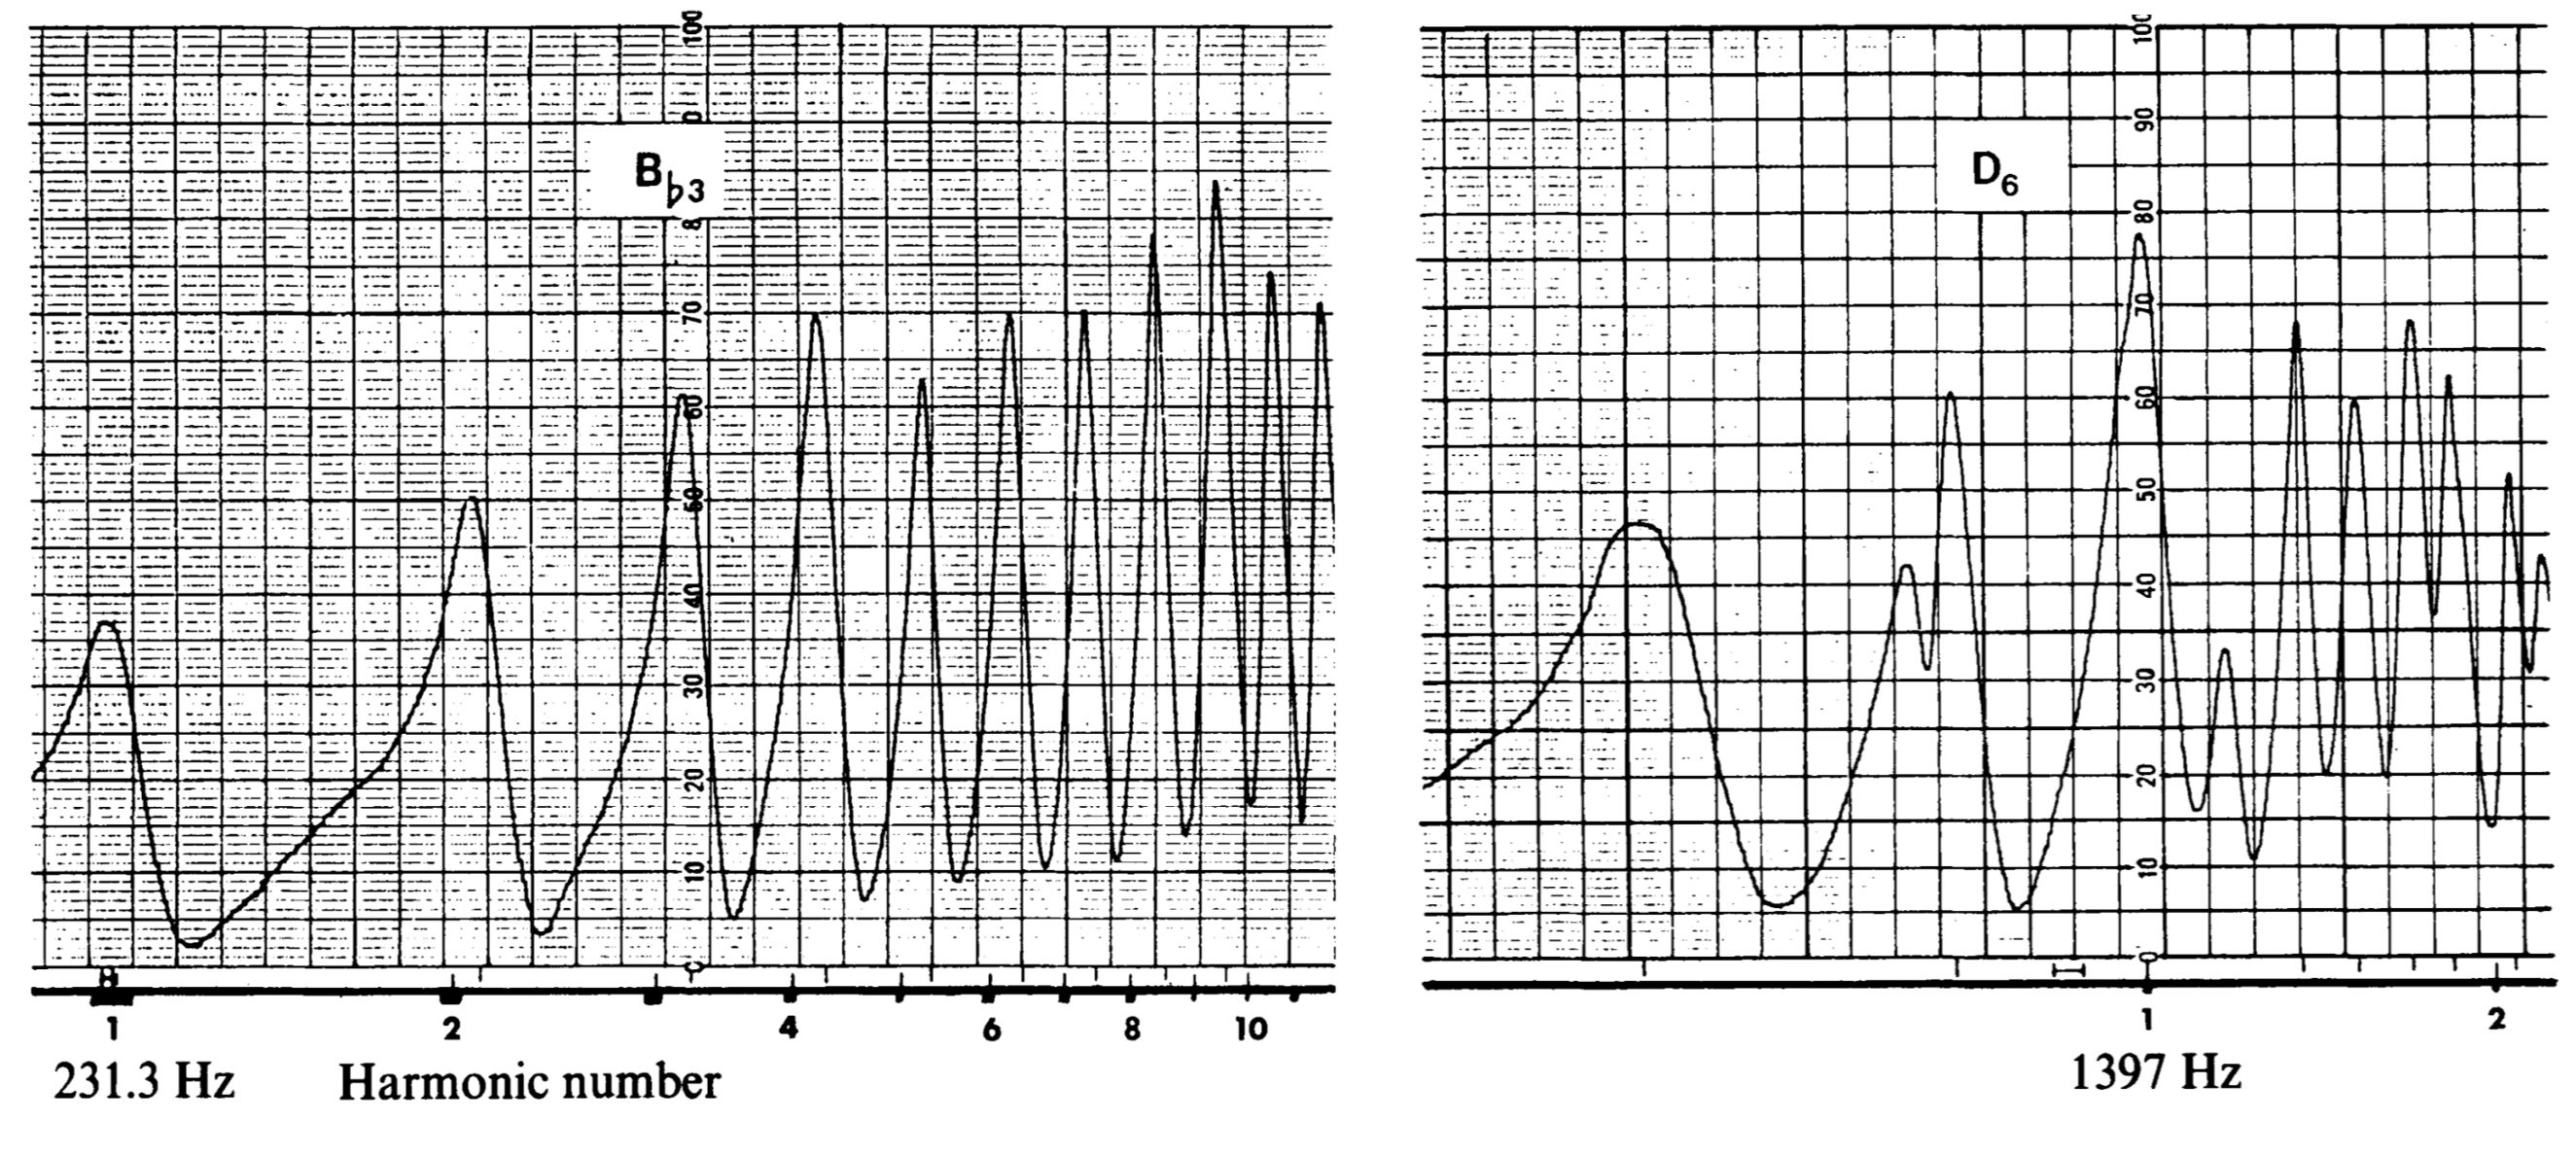
\includegraphics[width=0.7\linewidth]{00_Images/06_chapter/img74.jpg}
\caption{Oboe harmonic spectra in the low register versus a higher note}
\label{fig:oboe_harmonics_low_high}
\end{figure}

\paragraph{Bassoon} The bassoon is also a conical, double-reed instrument. To reach low notes, the tube is folded to obtain a total length of about \SI{2.6}{\meter}. Low notes can have a weak fundamental component because of the tube diameter. The tone is typically mellow and relatively poor in harmonics, which is associated with a low cutoff frequency in the range \SIrange{300}{600}{\hertz}. As for the oboe, the reed always beats, contributing to a limited tone-color change between soft and loud playing. 

\subsection{Saxophone}

The saxophone was designed by Adolphe Sax in the nineteenth century, with characteristics intentionally engineered rather than emerging from a long evolutionary process. It combines a wide conical bore, with flare semiangle around \SI{2}{\degree}, and a clarinet-like single reed. Large tone holes are operated by padded keys. A high cutoff frequency is paired with high radiation efficiency. Reflections are less pronounced than in other woodwinds, so stationary waves are less prominent, and radiation damping is strong for higher partials. A distinctive geometric feature is the sudden truncation of the conical shape at the mouthpiece. To preserve harmonic relationships, the mouthpiece is designed to mimic the acoustic behavior of the cone apex. Consequently, mouthpiece characteristics strongly affect the saxophone spectrum both below and above the cutoff frequency. 

    %! TEX rootmain.tex

\chapter{Jet-Switch Instruments}

Jet-switch instruments (flutes and flue organ pipes) share a common excitation principle: a thin air jet interacts with a sharp edge and an acoustic resonator. The chapter follows the physical chain from jet formation and instability, to jet-resonator coupling and the regenerative mechanism that sustains oscillation. Nonlinear effects, transients, mode transitions and aerodynamic noise are then introduced as natural consequences of the same feedback process, before closing with an overview of flute-type instrument families. 

\section{Dynamics of Air Jet}

\subsection{Jet Impingement on a Sharp Edge}

Even though the physical structure of these instruments varies a great deal, they all rely upon an air jet striking a sharp edge for excitation. The mechanics of a fluid jet entering an infinite body is a problem relevant in several application fields. Though conceptually simple, the underlying physics is complex and a first simplified treatment can be introduced by neglecting viscosity, compressibility and other non-idealities.

\paragraph{High-speed visualization} High-speed recordings of a jet striking a sharp edge show that the jet does not simply split into two steady streams. Instead, the impingement produces an unsteady roll-up of the shear layers and the formation of vortical structures close to the edge, so that the jet alternately feeds one side and then the other. This unsteady ``switching'' at the edge is the physical ingredient that later enables an oscillatory aeroacoustic source when the motion is synchronized with the resonator. This unsteady edge-switching is clearly visible in high-speed flow visualizations, as shown in figure \ref{fig:jet_edge_switching}.

\begin{figure}[!htb]
    \centering
    \subfloat{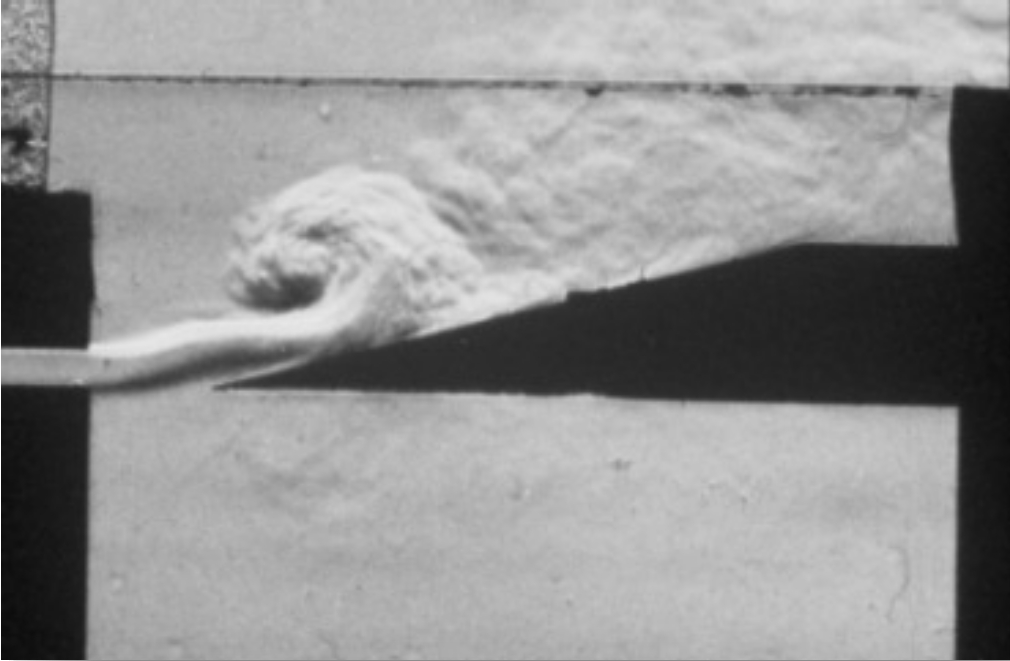
\includegraphics[width=0.3\linewidth]{00_Images/07_chapter/01_1.png}}\hfill
    \subfloat{
\includegraphics[width=0.3\linewidth]{00_Images/07_chapter/01_2.png}}\hfill
    \subfloat{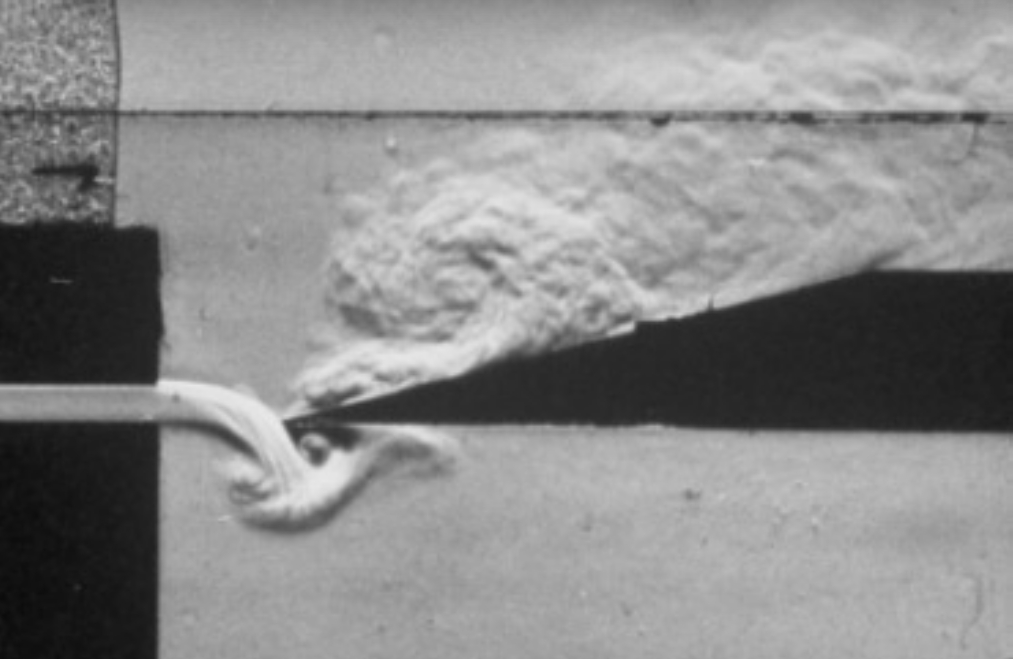
\includegraphics[width=0.3\linewidth]{00_Images/07_chapter/01_3.png}}
    \caption{High-speed visualization of jet switching at a sharp edge}
    \label{fig:jet_edge_switching}
\end{figure}

\subsection{Jet Instability and Convected Perturbations}

A qualitative analogy is provided by cigarette smoke. After a few centimeters, a thin smoke jet bends and oscillates and finally loses its organized structure, ending as a wide cloud. This kind of space-time instability can be observed as soon as two fluids with different velocities are in contact and it is greatly influenced by their relative velocity. In a flute, the air jet is blown across an open end of the pipe resonator. When jet oscillation occurs within the resonator, the jet instability can synchronize with the acoustic oscillation, resulting in a forced oscillation of the jet. The jet perturbation then grows as it is carried by the flow, being convected downstream toward the edge. 

\paragraph{Forced jet perturbation experiment} A clear illustration is obtained by forcing a transverse perturbation using loudspeakers placed a few centimeters apart from the flow, above and under it. In the reported setup the jet exhausts from the end of a \SI{1}{\milli\meter}-thick channel and the forced oscillation becomes visible as a growing waviness of the jet as it travels downstream. 

\subsection{Convection Velocity and Amplification}

Two characteristics of the jet motion are important for flue oscillation:

\begin{enumerate}
    \item the convection velocity of the perturbation, corresponding to the propagation velocity of the perturbation waves on the jet, which to a first approximation is about half the centerline jet velocity
    \item the amplification of the perturbation, corresponding to a characteristic growth factor of the instability waves along the jet
\end{enumerate}

Both characteristics depend on frequency, but the amplification depends strongly on it. The jet instability is stronger in a frequency range that depends on both jet velocity and jet thickness and the strongest amplification appears for frequencies around
\[
\frac{0.3U_j}{h}
\]
where \( U_j \) is the jet velocity and \( h \) is the thickness of the flue channel from which the jet is flowing. 

\section{Sound Generation}

Three main phenomena are involved in sound generation:

\begin{itemize}
    \item the perturbation of the jet by the acoustic field (jet receptivity)
    \item the evolution of the perturbation convected by the jet (jet instability)
    \item the production of acoustic energy by the perturbed flow (aeroacoustic sources)
\end{itemize}

The process can be summarized as a feedback loop: the pipe provides passive resonance and generates an acoustic field that perturbs the jet; the jet supports propagation and amplification of that perturbation while it is convected toward the edge; at the labium the perturbed jet acts as an aeroacoustic source that injects acoustic energy into the resonator, closing the loop. 

\section{Disturbance of an Air Jet}

\subsection{Terminology}

A reference terminology can be introduced using the recorder geometry. The air supply pressure is provided by the player’s mouth and drives a jet through the flue channel. The jet emerges at the flue exit and interacts with the labium, while the downstream pipe constitutes the resonator. The opening between the flue exit and the labium is called the mouth. Different names are adopted for organ pipes and transverse flutes, but the functional elements remain the same. The reference geometry and the associated naming conventions are summarized in figure \ref{fig:recorder_geometry_terms}.

\begin{figure}[!htb]
    \centering
    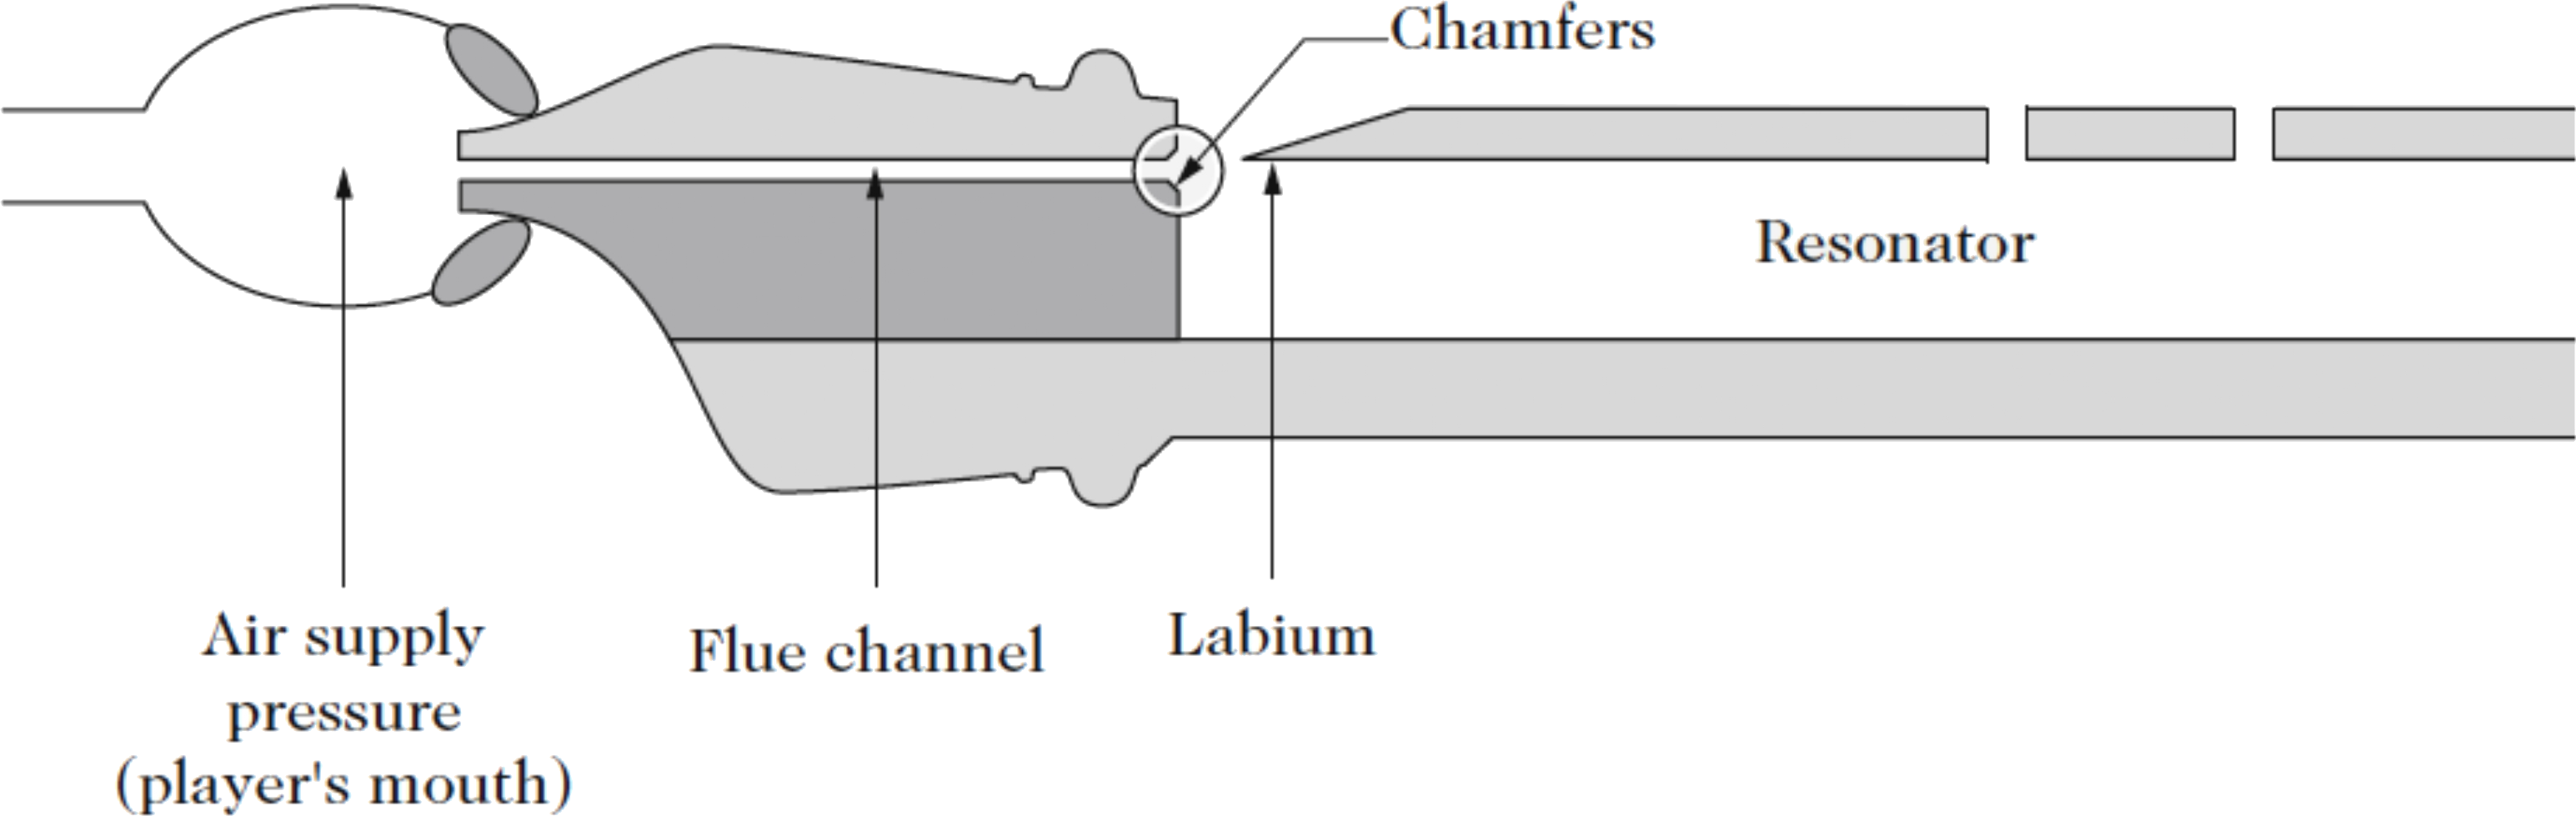
\includegraphics[width=0.7\linewidth]{00_Images/07_chapter/02.png}
    \caption{Recorder-like geometry and terminology for jet-switch instruments}
    \label{fig:recorder_geometry_terms}
\end{figure}

\subsection{Acoustic Sources at the Labium of the Flute}

The acoustic field at the flue exit induces a perturbation of the jet, which is amplified while being convected toward the labium. This process results in a transverse oscillation of the jet from one side of the labium to the other. A loop description makes the coupling more explicit. The acoustic field in the pipe resonator is responsible for the initial jet perturbation. The perturbation is then convected and amplified downstream due to the natural jet instability. The interaction of the perturbed jet with the labium constitutes the aeroacoustic source that feeds acoustic energy into the pipe. As a response to this excitation, the acoustic energy in the pipe is associated with an acoustic flow through the mouth, which in turn produces the jet perturbation at the flue exit, closing the feedback loop. 

\section{The Regenerative Excitation Mechanism}

\subsection{The Self-Sustained Oscillator as a Looped System}

The loop description allows predicting the oscillation frequency. Because the pipe accumulates energy only at resonances, the oscillation takes place at a frequency close to a passive pipe resonance. Stationary oscillations can occur when the total phase shift around the loop is \( 2\pi \) or any multiple of it. In a recorder gently blown, the time delay associated with the convection of perturbations is about half of the oscillation period, so the phase shift of the pipe must provide the complement to \( 2\pi \). For moderate blowing, the jet velocity increases and the convection delay decreases, so the delay associated with the pipe must increase. When blowing harder, the convection delay becomes too small compared to the period of the first pipe resonance and the oscillation jumps to the second pipe resonance, for which the same convection delay represents a larger phase shift. This regime jump is called overblowing. By blowing gently at very low pressures compared to standard playing, very soft tones can be produced at frequencies close to pipe resonances. This playing technique, called whistle-tones or sometimes eolian tones, corresponds to convection delays on the jet that are larger than one oscillation period. Values around one and a half or two and a half periods may be observed, instead of the half period typical of standard playing conditions. 

\subsection{Overblowing}

A simplified representation of the playing frequency of a flute as a function of jet velocity shows that oscillation occurs at a frequency close to one of the passive pipe resonances \( f_{1} \), \( f_{2} \), or \( f_{3} \). Regime changes do not occur at the same jet velocity when the jet velocity is increased versus decreased and a hysteresis appears. Dotted branches indicate whistle-tone oscillations. The typical evolution of the playing regime with jet velocity, including hysteresis and whistle-tone branches, is illustrated in figure \ref{fig:overblowing_hysteresis}.

\begin{figure}[!htb]
    \centering
    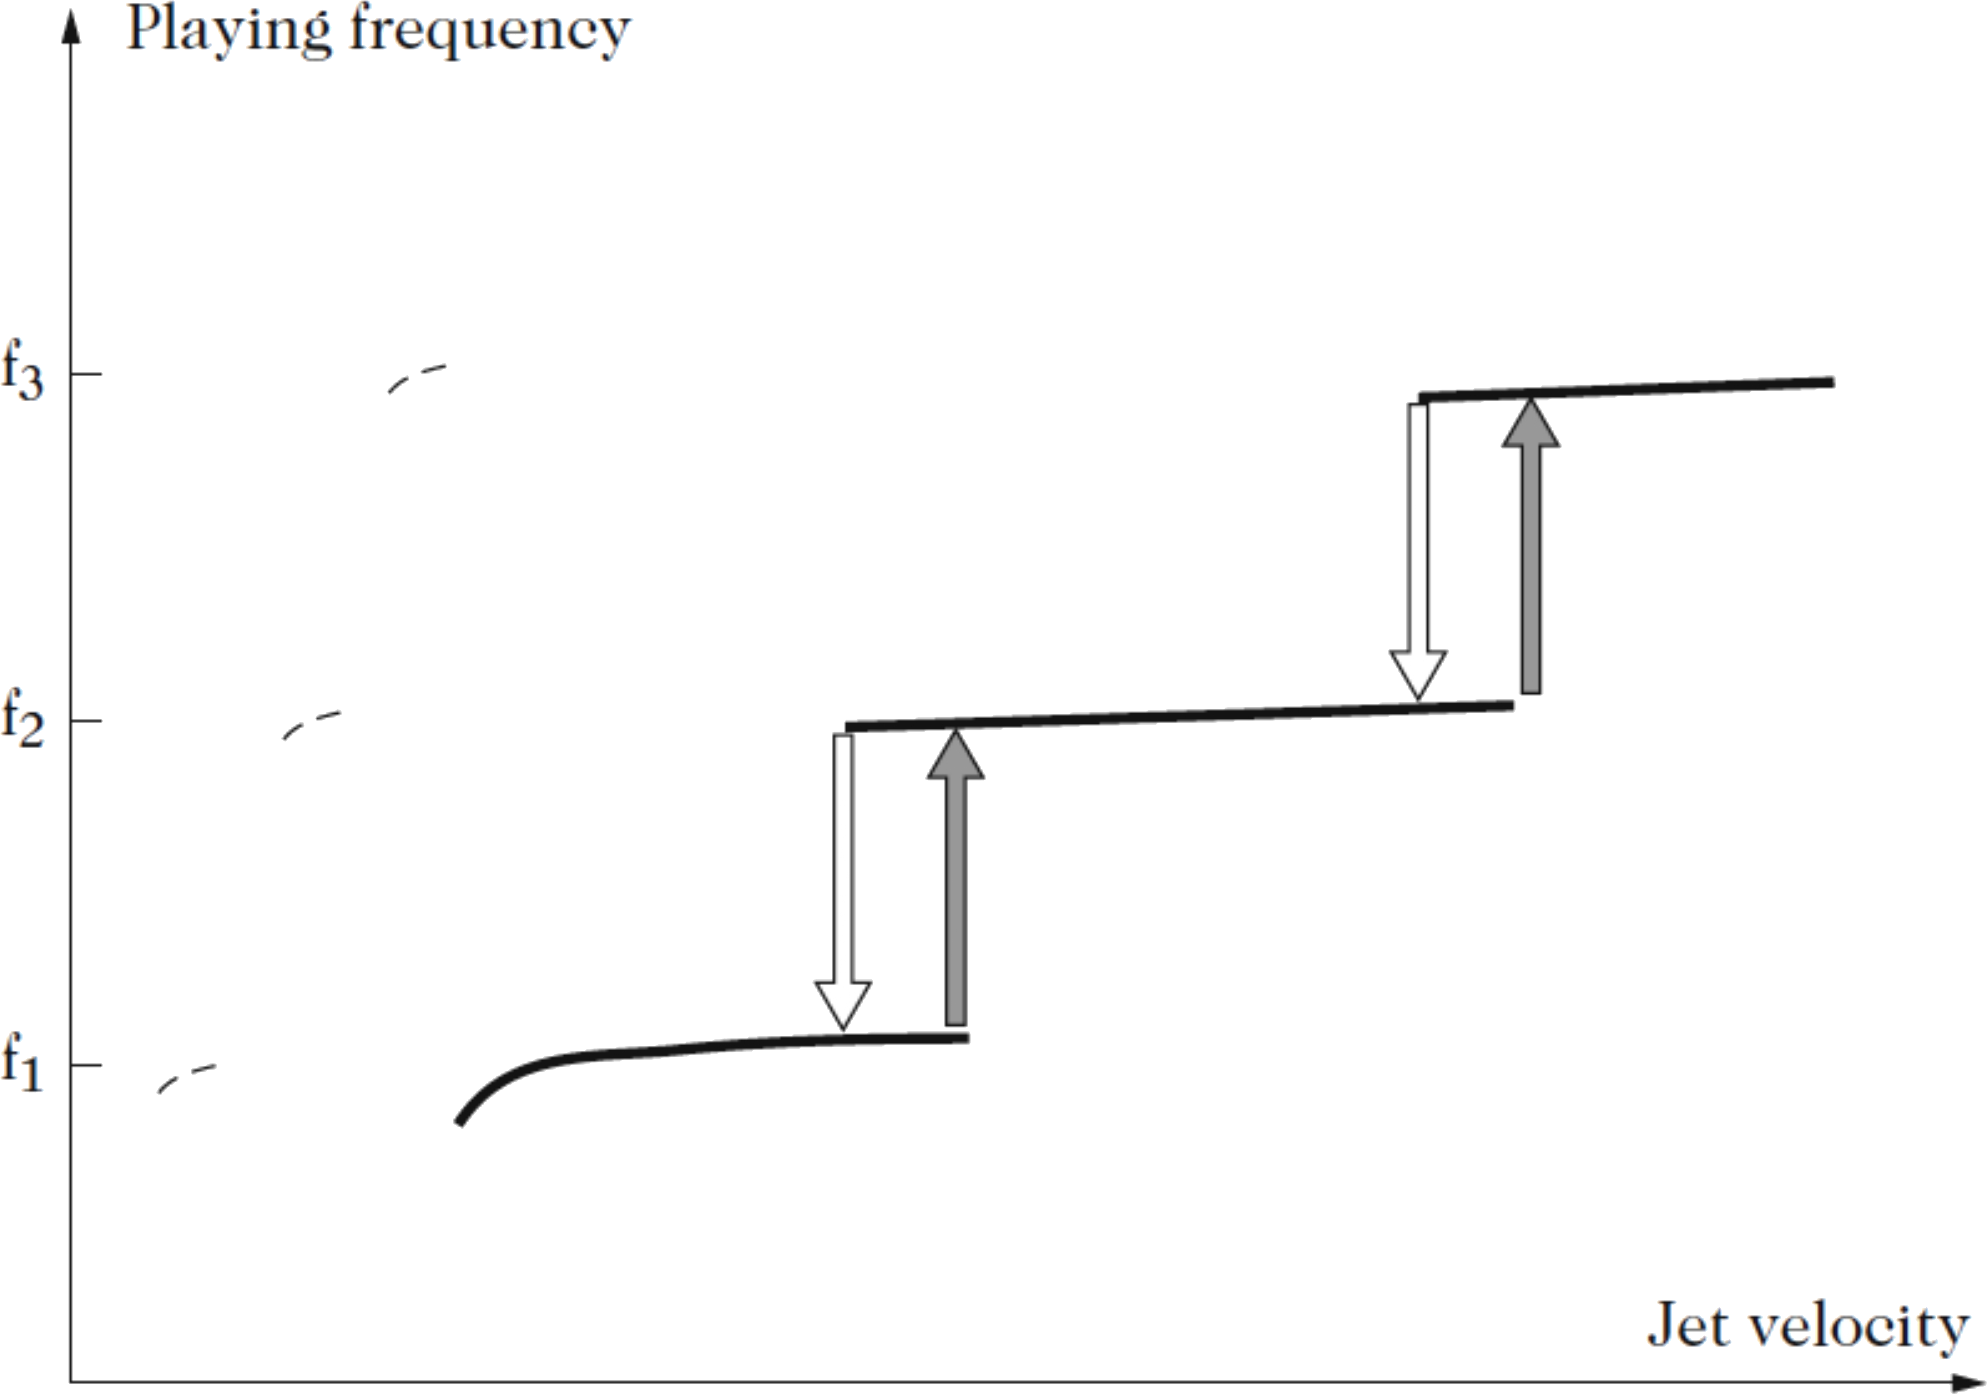
\includegraphics[width=0.7\linewidth]{00_Images/07_chapter/04.png}
    \caption{Overblowing and hysteresis of oscillation regimes versus jet velocity}
    \label{fig:overblowing_hysteresis}
\end{figure}

\section{The Sound of Flutes}

Using a mechanical air supply allows producing a stationary sound, as for an organ. The sound radiated by a pipe blown in this way can be split into two contributions: a deterministic part, analyzed in terms of sine-wave components and a stochastic part generated by turbulence. Turbulence produces broadband noise that is filtered by the pipe acoustical response. FFT analyses of internal pressure and radiated pressure measured at a distance of \SI{30}{\centi\meter} in front of the mouth of a small organ pipe illustrate this separation. At frequencies higher than the fifth harmonic, around \SI{2.5}{\kilo\hertz}, resonances can be identified through their filtering effect on the turbulence noise, because their frequencies do not coincide any more with the harmonic lines. The shift between harmonics and pipe resonances is visible, for example, when the sixth resonance lies between the harmonic lines 6 and 7. When the air supply comes from a player rather than from a mechanical system, pressure fluctuations modulate sound production. Vibrato corresponds to a conscious modulation of blowing, but fluctuations are also observed when the player aims at producing a stable tone. Because of these fluctuations, it is generally not possible to define a stationary part of the tone. Starting transients are also difficult to analyze: the sound components that later become the harmonics of the steady part display changing frequencies and amplitudes during the attack transient. In the reported example of the time evolution of the first three frequency components, the second component, with frequency close to twice that of the later fundamental, increases much faster than the first component. The deterministic harmonic lines and the turbulence-driven broadband component can be distinguished in measured spectra, as shown in figure \ref{fig:pipe_fft_deterministic_stochastic}, where a time evolution of the first three frequency components during an attack transient is also reported.

\begin{figure}[!htb]
    \centering
    \subfloat[Spectra]{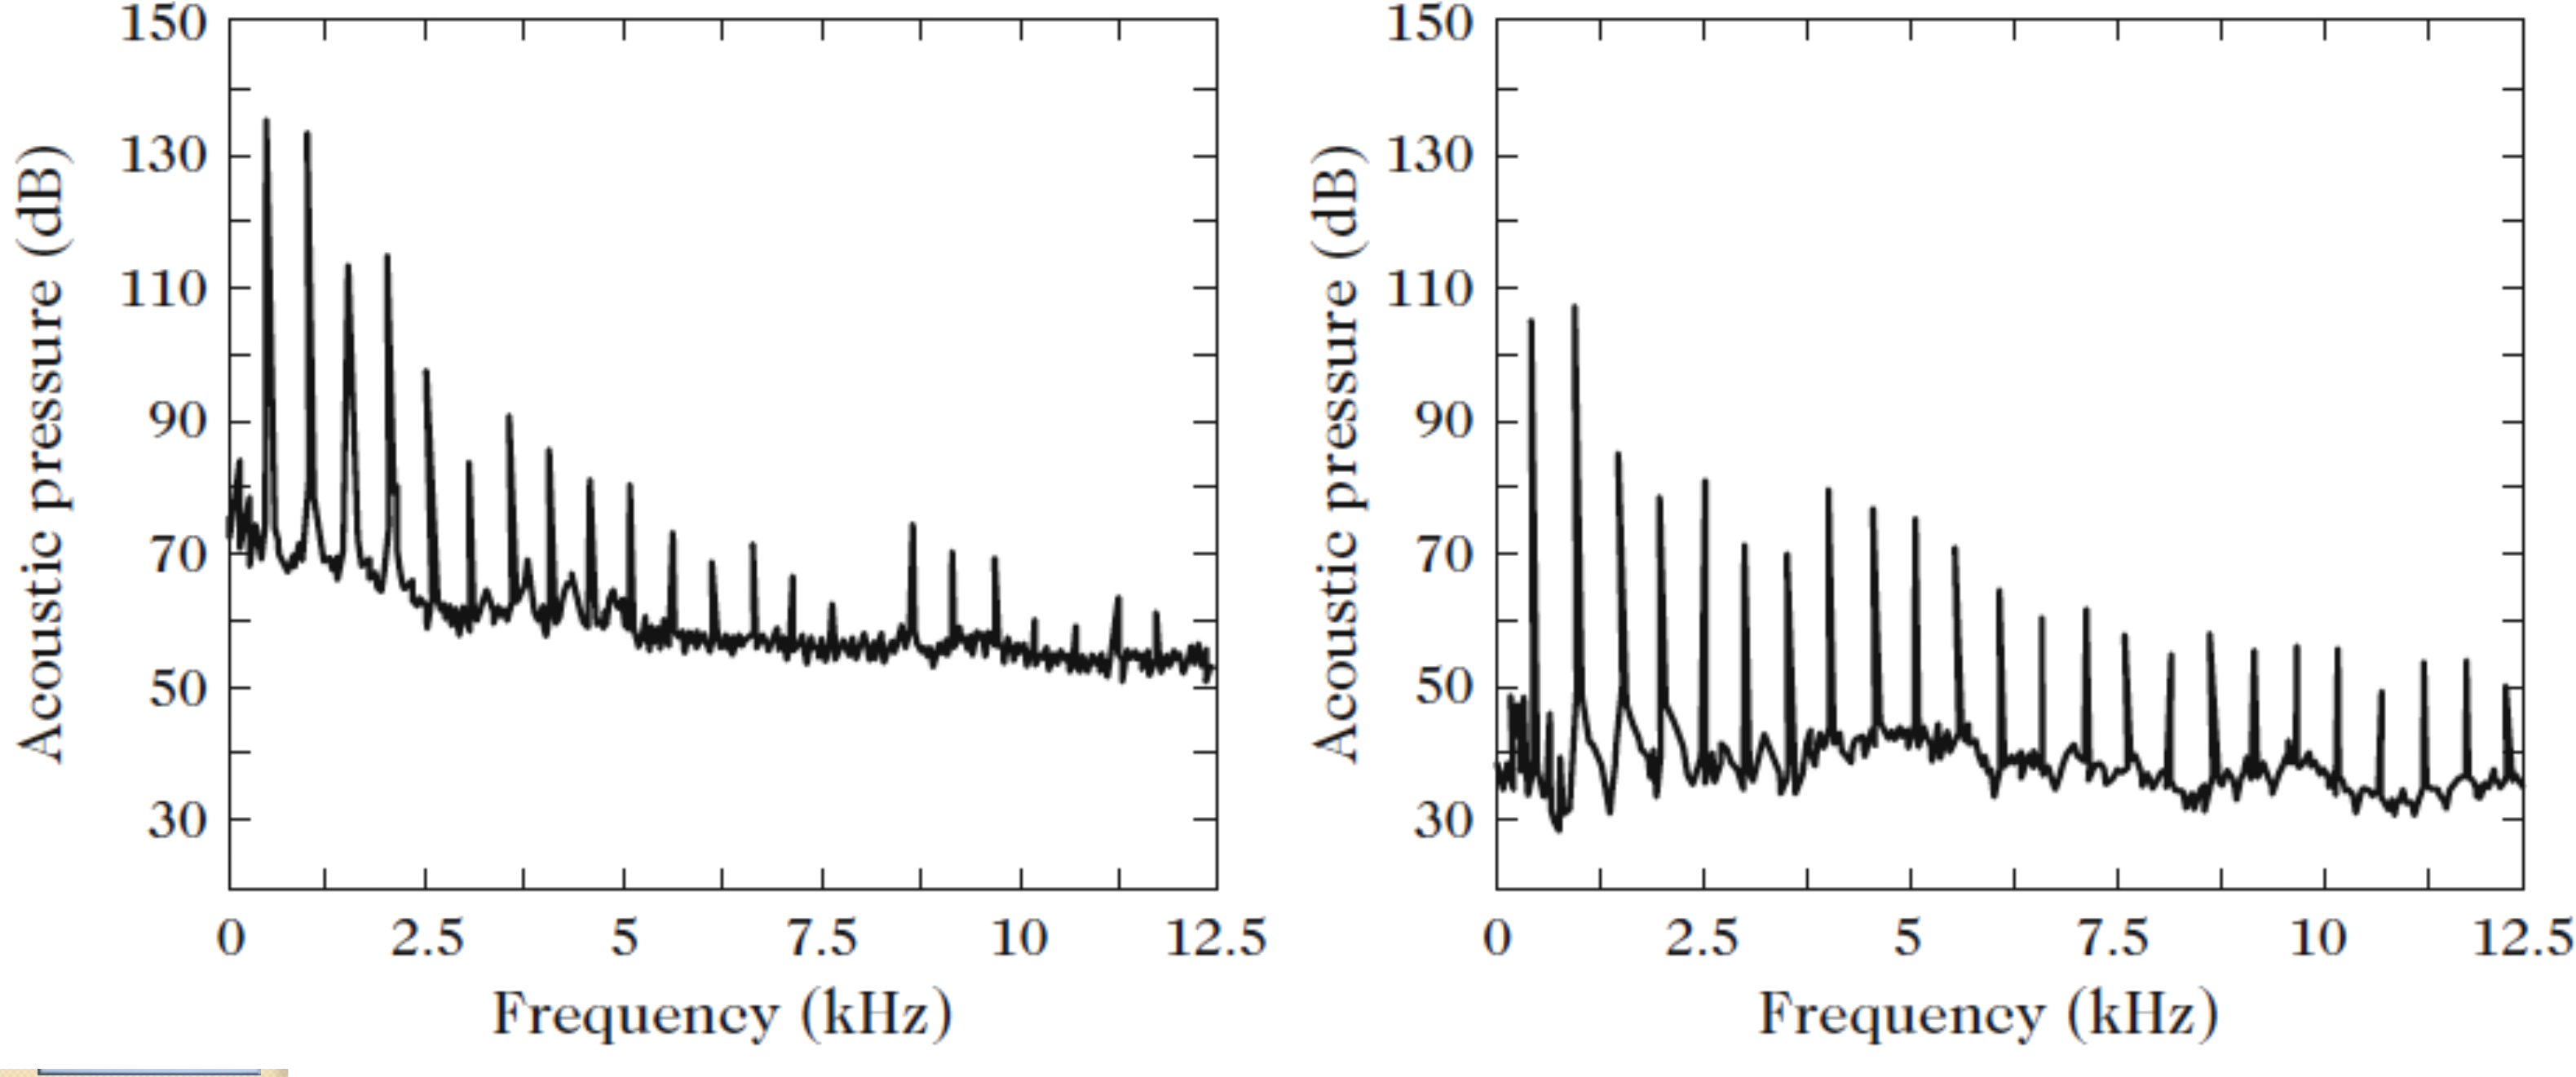
\includegraphics[height=0.17\textheight]{00_Images/07_chapter/05.png}}
    \subfloat[Time evolution]{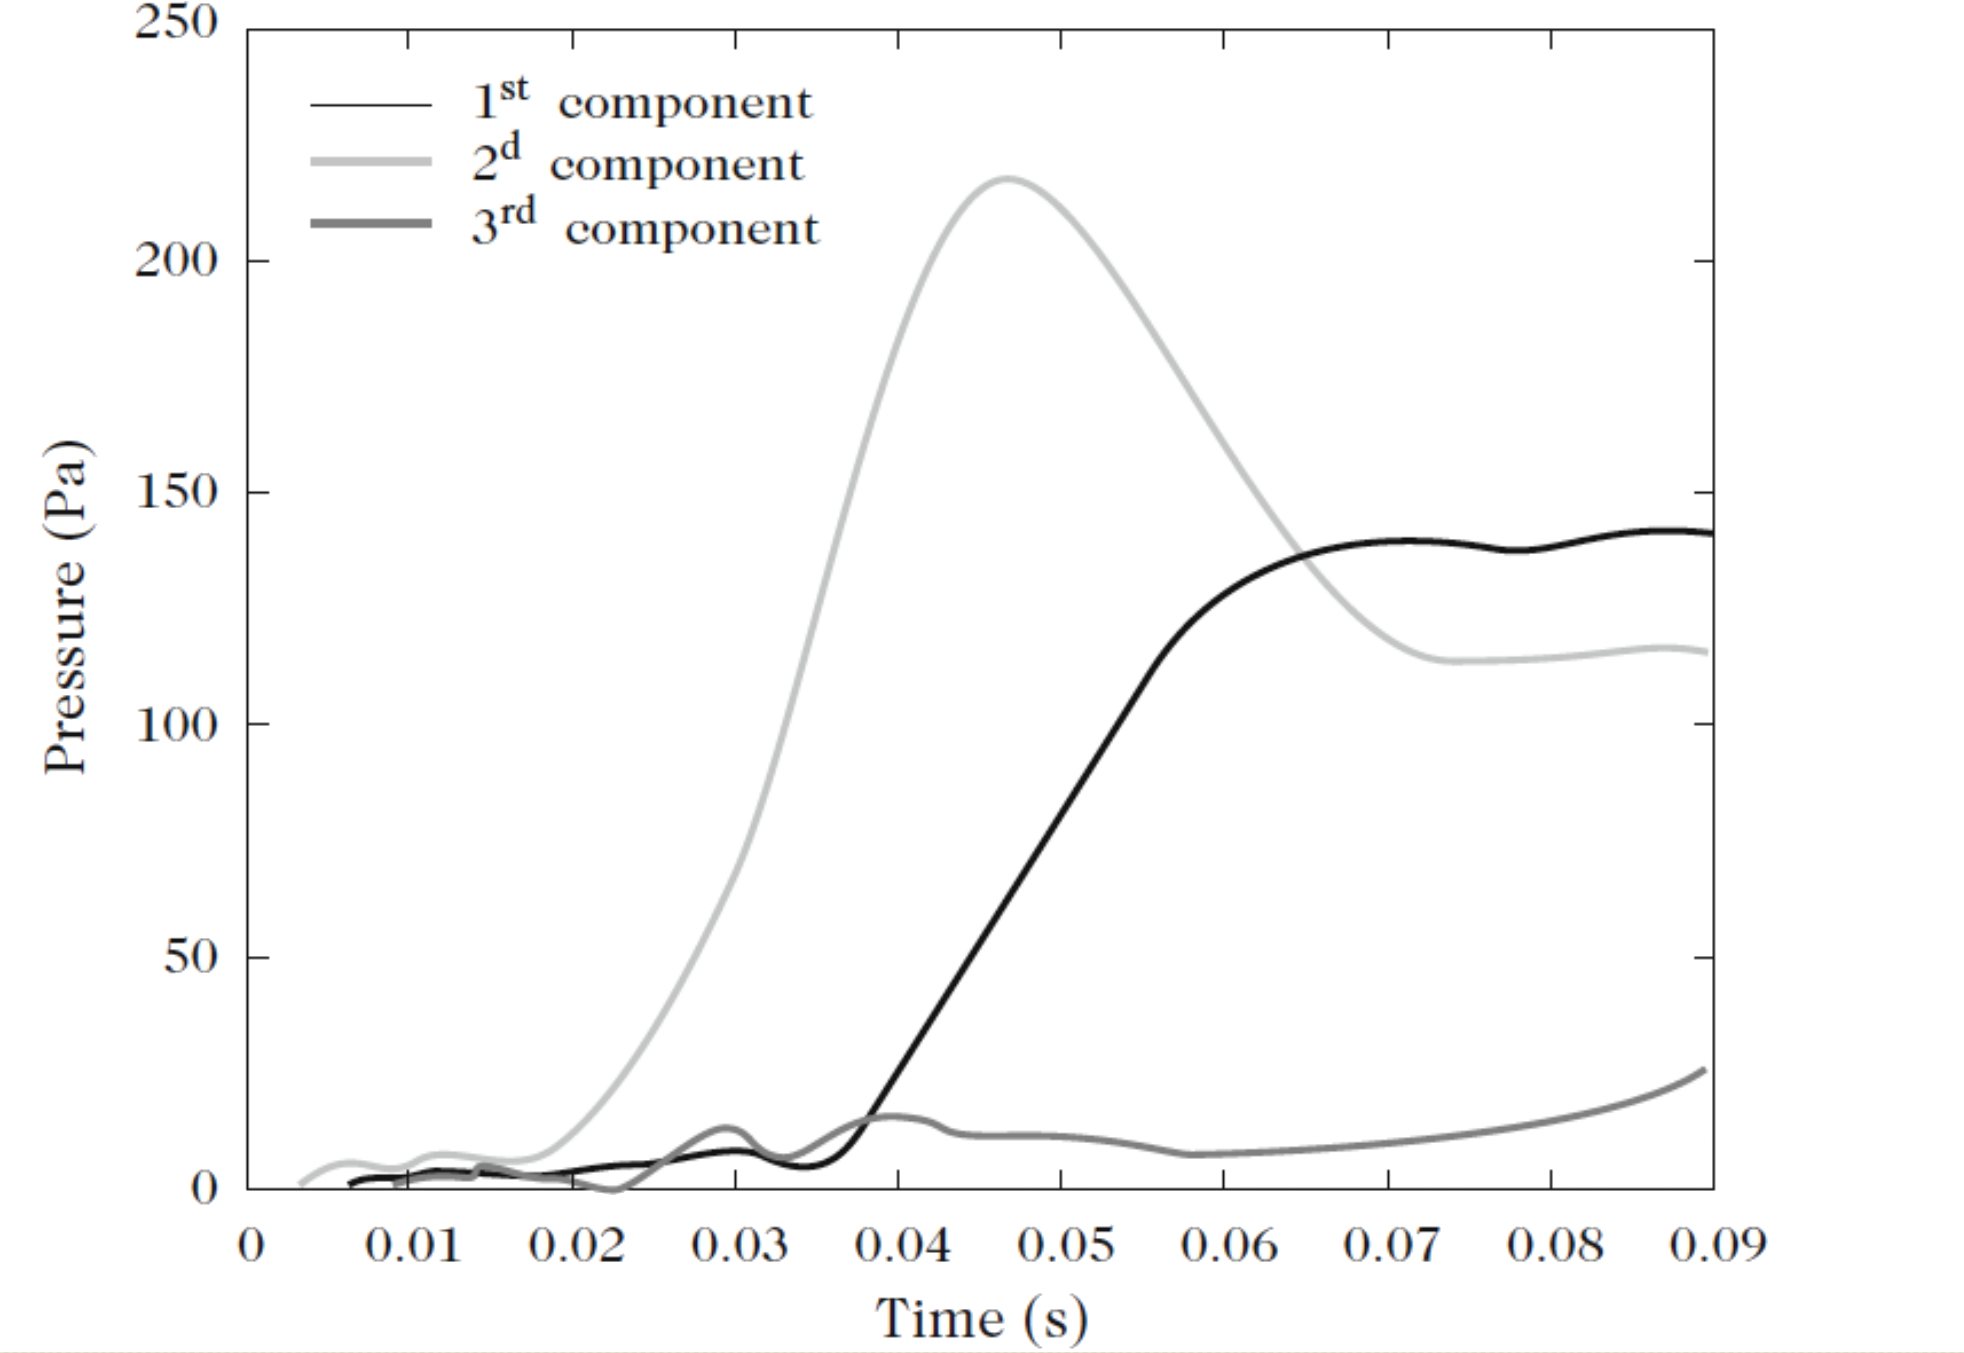
\includegraphics[height=0.17\textheight]{00_Images/07_chapter/06.png}}
    \caption{Measured spectra and time evolution showing harmonic components and turbulence noise filtered by resonances}
    \label{fig:pipe_fft_deterministic_stochastic}
\end{figure}

\section{Jet-Resonator Interaction}

\subsection{A Global Model of the Instrument}

A global model is most straightforward for jet-driven instruments whose geometry remains essentially fixed during playing, such as flue organ pipes and recorders. In this case, the excitation system can be described by a small set of stable parameters (channel geometry, jet velocity, flue exit--labium distance) coupled to the passive acoustic response of the resonator. Transverse flutes are more complex because the jet is shaped by the player’s lips, so the effective geometry and jet parameters can vary continuously during performance and become part of the control strategy. 

\subsection{Parameters of the Model}

\begin{figure}[!htb]
    \centering
    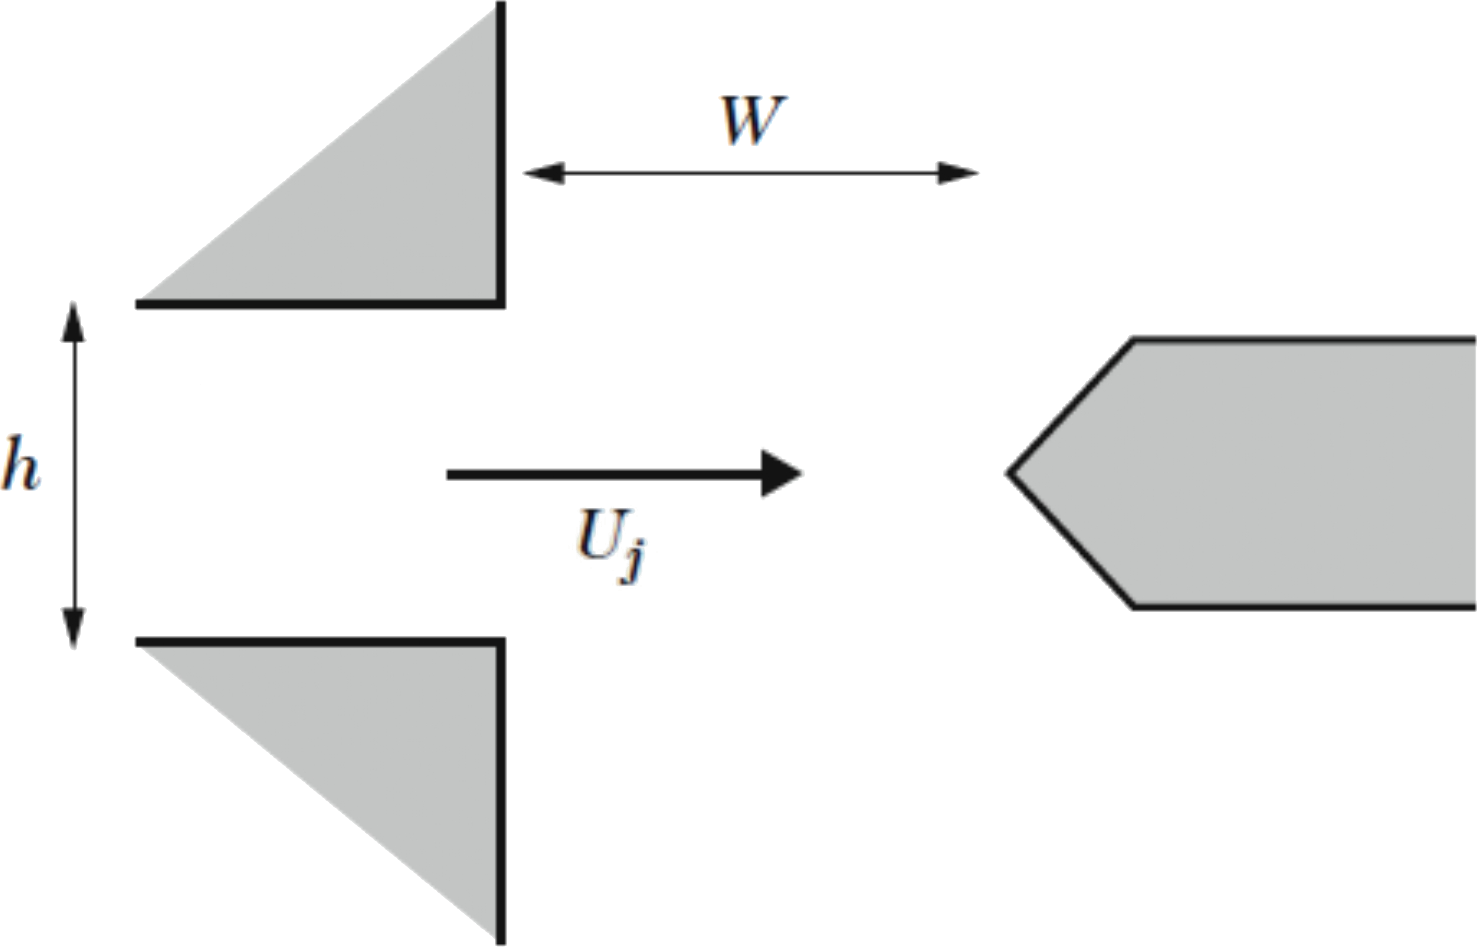
\includegraphics[width=0.5\linewidth]{00_Images/07_chapter/07.png}
    \caption{Simplified geometry}
    \label{fig:geom}
\end{figure}

A minimal geometric (reported in figure \ref{fig:geom}) and flow description introduces the channel thickness \( h \), the central jet velocity at the channel exit \( U_j \) and the flue exit--labium distance \( W \). The transverse jet displacement can be decomposed as
\[
y(x,t) = y_{0}(x,t) + y_{\mathrm{ac}}(x,t)
\]
and the corresponding transverse velocity as
\[
v(x,t) = v_{0}(x,t) + v_{\mathrm{ac}}(x,t)
\]
The jet regime is characterized by the Reynolds number
\[
\Re\{y\} = \frac{U_j h}{\nu}
\]
where \( \nu \) is the kinematic viscosity. Typical values range from a few hundreds (recorder) up to about \( 10^{4} \) in modern transverse flute playing, with
\[
500 < \Re\{y\} < 10000
\qquad
\nu = \SI{1.5e-5}{\meter\squared\per\second}
\]
Jet instability is characterized by a Strouhal number (inverse dimensionless frequency). Two common definitions are
\[
\frac{\omega W}{U_j}
\qquad
\frac{fh}{U_j}
\]
For normally blown flutes, one half hydrodynamic wavelength is observed between flue exit and labium, leading to
\[
\mathrm{St}_{W} = \frac{fW}{U_j} \approx 0.25
\]
A convenient measure of oscillation level is the ratio between the acoustic perturbation velocity in the mouth and the central jet velocity, typically
\[
\frac{V_{\mathrm{ac}}}{U_j} \approx 10^{-1}
\]

\subsection{The Flow in the Channel}

Knowing the overpressure \( \Delta p \) in the reservoir (player’s mouth) with respect to atmospheric pressure leads to an estimate of the central jet velocity,
\[
U_j = \sqrt{\frac{2\Delta p}{\rho_0}}
\]
The Bernoulli estimate holds at the center of the flow. Near the walls, viscosity produces boundary layers whose thickness at position \( x \) along the channel is approximated by
\[
\delta(x) \approx \sqrt{\frac{\nu x}{U}}
\]
In a short channel, boundary layers remain confined near the walls and the central part of the flow exhibits an approximately uniform velocity profile. In a long channel, the two boundary layers merge and a parabolic (Poiseuille) profile develops. In most flutes, the Bernoulli approximation (uniform velocity) is a reasonable working model. 

\subsection{The Jet Flowing out of the Channel}

At the channel inlet, the flow has an approximate top-hat velocity profile. As the fluid flows downstream, boundary layers thicken because of viscosity. If the channel outlet is rounded, the flow slows down, producing an increase of pressure. The change of sign of the pressure gradient in the diverging part at the channel exit is responsible for flow separation. Because of viscosity, the free jet entrains the surrounding fluid. This behavior is reported in figure \ref{fig:jetflowing}.

\begin{figure}[!htb]
    \centering
    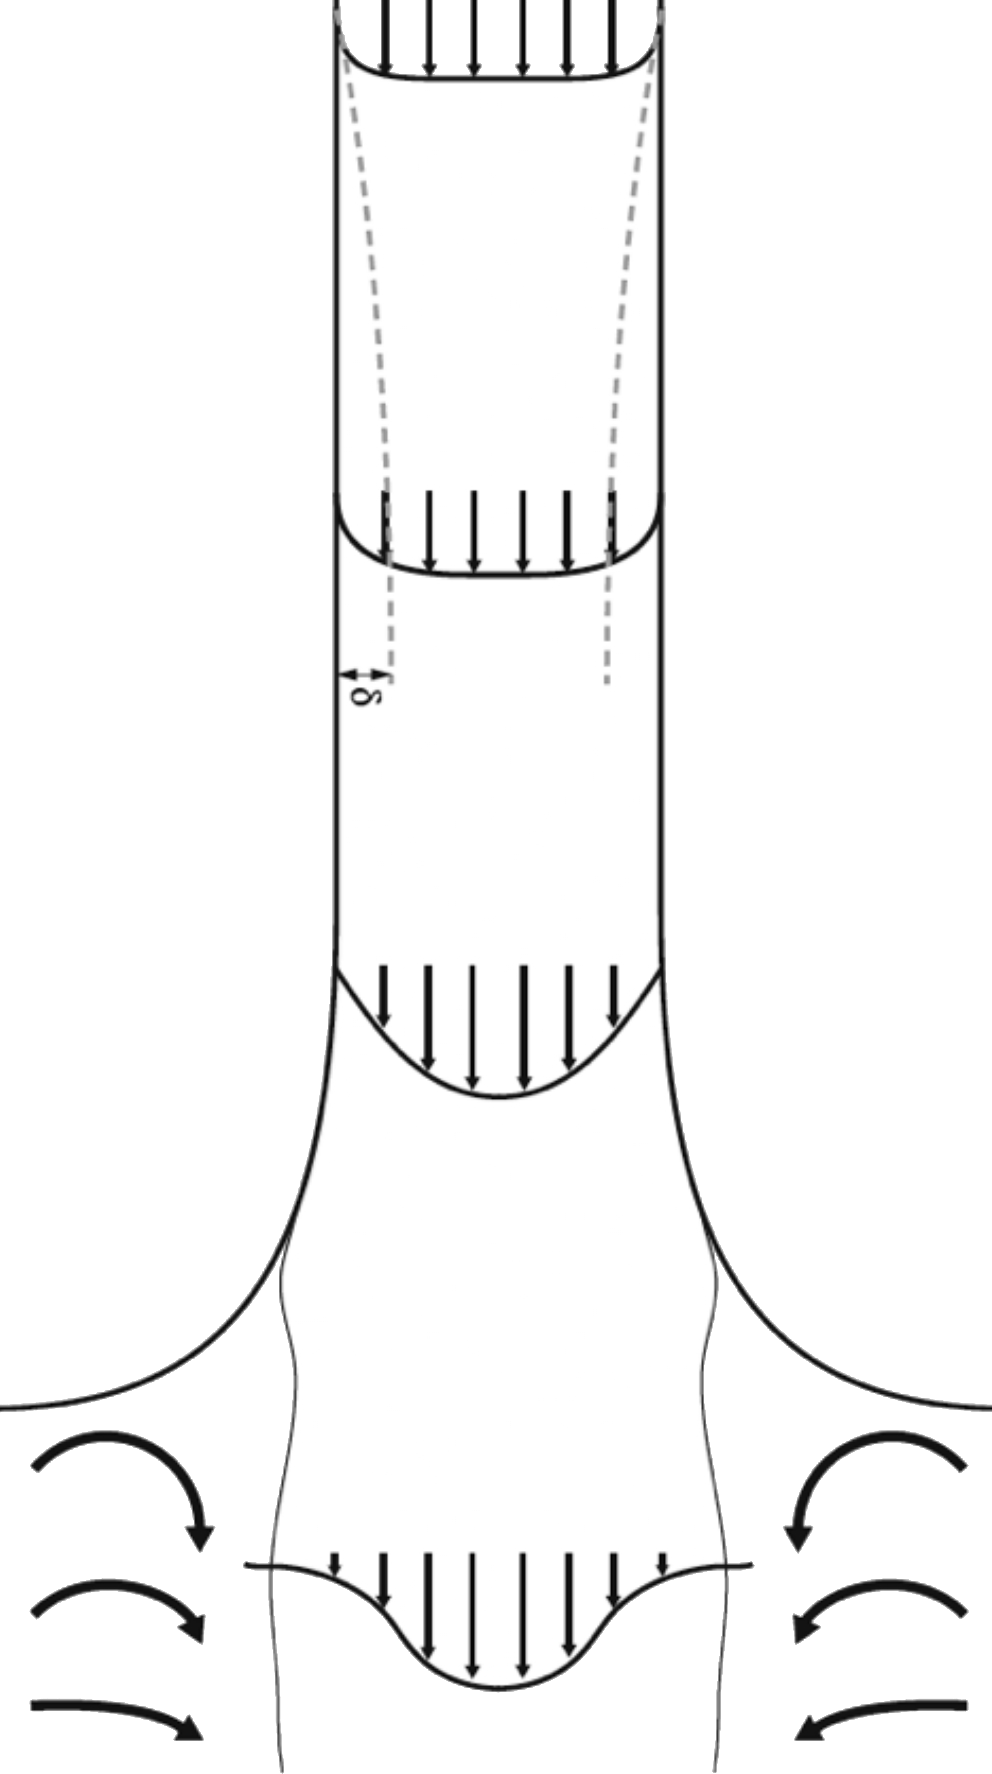
\includegraphics[height=0.7\linewidth,angle=90]{00_Images/07_chapter/10.png}
    \caption{Jet flowing out of the channel}
    \label{fig:jetflowing}
\end{figure}

\section{Jet Instability}

\subsection{Assumptions}

A first physical description of jet instability is introduced under the following assumptions:

\begin{itemize}
    \item inviscid fluid
    \item compressibility can be ignored, which is justified
    \begin{itemize}
        \item as long as the jet velocity \(U\) is kept small compared to the sound speed \(c\)
        \item as long as the dimensions of the jet and sound production region are small compared to the acoustic wavelength
    \end{itemize}
\end{itemize}

\subsection{Kelvin-Helmholtz Instability}

Let us start the physical analysis of the jet instability with a simple case: the flow at the planar interface between two areas of the fluid with different velocities. This is known as the Kelvin-Helmholtz instability. This flow can be described by the relative velocity \(U\) between the two areas,
\[
v_x = \frac{U}{2} \quad \text{if } y>0
\qquad
v_x = -\frac{U}{2} \quad \text{if } y<0
\qquad
v_y = 0
\]

\subsection{The Instability Mechanism}

The instability mechanism of a perturbed shear layer can be summarized as follows (and visualized in figure \ref{fig:instmech}):
\begin{itemize}
\item a perturbation of the interface induces local convection that concentrates the vorticity at points \(C\)
\item this concentration amplifies the initial perturbation, leading to the formation of rolled structures
\item vorticity accumulation induces asymmetrical velocities that further amplify the initial perturbation, up to the point where waves break
\end{itemize}

\begin{figure}[!htb]
    \centering
    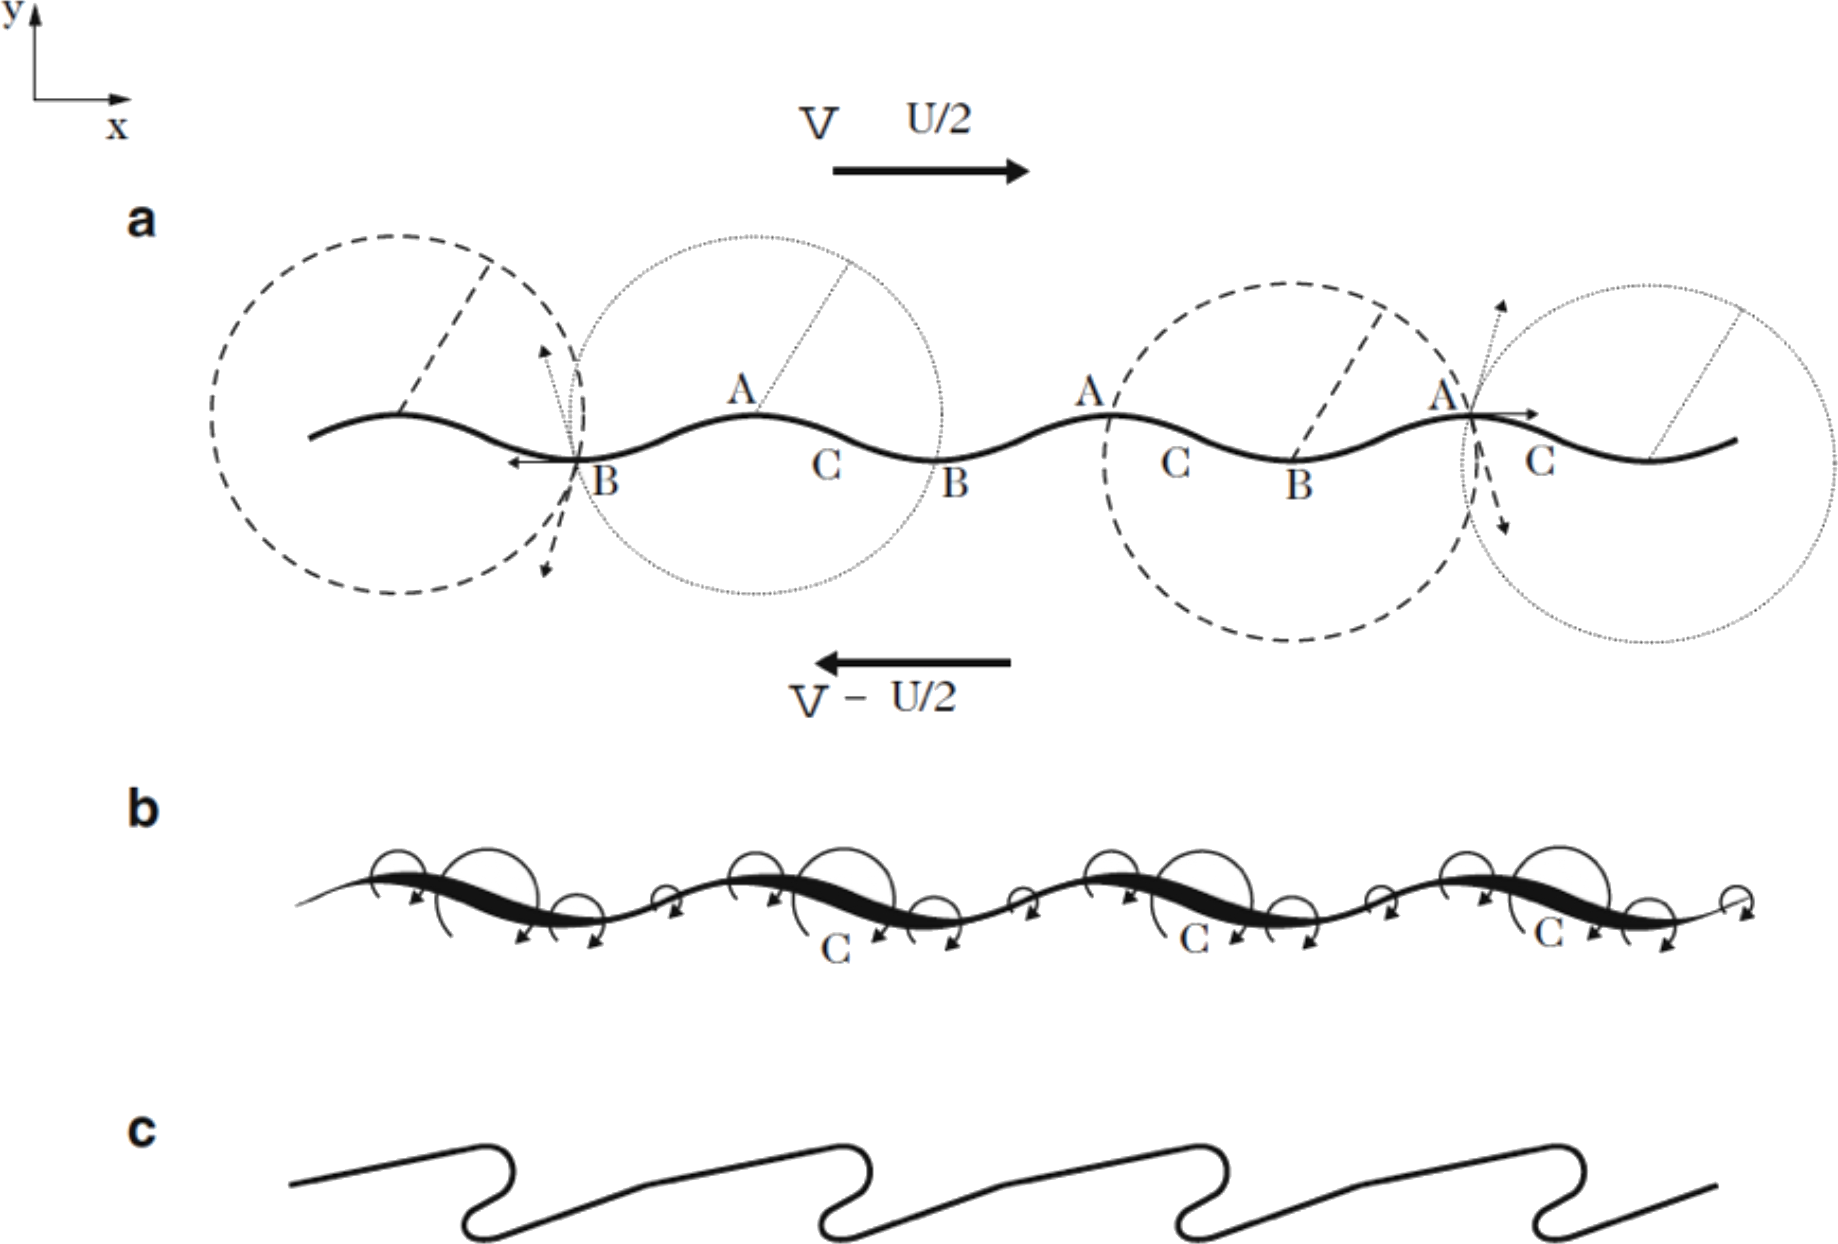
\includegraphics[width=0.7\linewidth]{00_Images/07_chapter/11.png}
    \caption{Instability mechanism}
    \label{fig:instmech}
\end{figure}

\subsection{Instability of an Infinite Jet}

If the jet velocity profile is symmetrical about \(y=0\), perturbations on both shear layers of the jet can be symmetrical or anti-symmetrical, depending on the symmetry properties of the initial perturbation of the jet.

\begin{itemize}
    \item Symmetrical perturbations induce the so-called varicose oscillations of the jet, associated with a modulation of the jet thickness.
    \item Anti-symmetrical perturbations correspond to sinuous oscillations of the jet. Sinuous oscillations have a stronger amplification than varicose oscillations.
\end{itemize}

Jet visualizations in various flute configurations indicate that the sinuous motion dominates under standard blowing conditions. The distinction between varicose and sinuous oscillations is summarized by the mode sketches in figure \ref{fig:varicose_sinuous_modes}.

\begin{figure}[!htb]
    \centering
    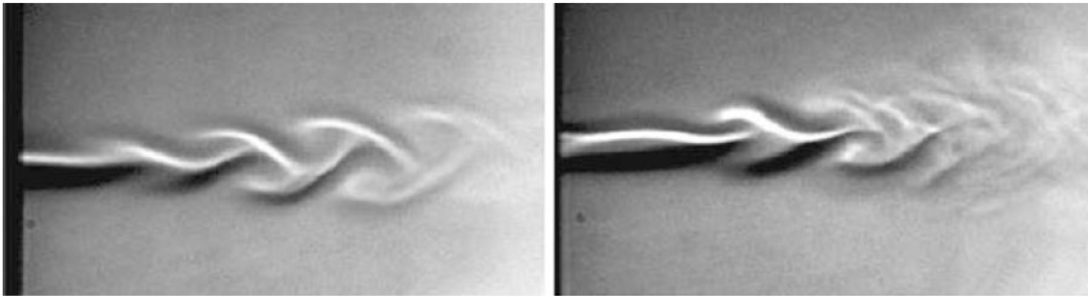
\includegraphics[width=0.7\linewidth]{00_Images/07_chapter/12.png}
    \caption{Varicose and sinuous jet oscillation modes}
    \label{fig:varicose_sinuous_modes}
\end{figure}

\subsection{Spatial Amplification}

It is of interest the study of the spatial amplification of the instability. Introducing a complex wavenumber,
\[
\alpha = \alpha_r + j\alpha_i
\]
the amplitude of the oscillation is proportional to
\[
e^{\alpha_i x}
\]
where \( \alpha_i \) is the spatial growth rate and \( \alpha_r \) controls the space periodicity. The amplification depends on the jet velocity profile and corresponds to anti-symmetrical jet oscillations (sinuous) or symmetrical oscillations (varicose), with sinuous oscillations being better amplified than varicose oscillations.

\section{Jet Receptivity}

\subsection{Localization of the Initial Perturbation}

The way the acoustic field produces the initial jet perturbation is called the receptivity. To a first approximation, the initial perturbation is assumed to be localized at the flue exit. In an incompressible inviscid flow approximation, this can be justified by vorticity conservation in the flow. The jet perturbation can be represented as a modulation of vorticity in the flow. Because of vorticity conservation, such a vorticity modulation can only be injected at the separation points of the flow, due to local viscous effects. The amplification that occurs downstream is only a consequence of the jet instability, in terms of redistribution of the initial vorticity.

\subsection{Influence of Geometry}

Details of the geometry and of the flow in the vicinity of the flow separation points can strongly affect the receptivity:

\begin{itemize}
    \item boundary layer thickness in the channel just upstream from the flue exit
    \item geometry of the channel exit
\end{itemize}

This is in line with recorder makers’ care in cutting chamfers at the end of the channel and with transverse flute players’ observation that small irregularities on the lips strongly affect tone quality.

\subsection{Semi-Infinite Jet Model}

The theory behind varicose and sinuous motions is valid for an infinite parallel flow. In flutes, the jet is formed at the flue exit and flows through a window where strong transverse acoustic flows can be experienced, due to the accumulation of acoustical energy in the pipe resonator. A first step is to consider a semi-infinite jet with negligible transverse displacement at the flue exit. The transverse displacement \( \eta(x,t) \) of the jet in the \(y\) direction can be calculated by integration of the transverse velocity from the flue exit to the current position \(x\) in the mouth. This transverse velocity is made of two components: a perturbation term \(v'_y\) exponentially growing with the distance from the flue exit and the air displacement due to the acoustic velocity \(v_{\mathrm{ac}}\),
\[
\eta(x,t)=\int_{t-x/U_0}^{t}\Bigl[v'_y(x',t')+v_{\mathrm{ac}}(x',t')\Bigr]dt'
\qquad
x' = x - (t-t')U_0
\]

\subsection{Exponential Growth}

For long enough distances from the flue exit, one can ignore the contribution of the acoustic displacement. The transverse jet displacement then writes
\[
\eta(x,t)\approx -\int_{t-x/U_0}^{t}\frac{\partial\psi'(x',t')}{\partial x}dt'
\]
where \( \psi' \) is the perturbation amplification function. This implies an exponential growth of the amplitude of the jet displacement.

\subsection{Experimental Model of Receptivity}

A good experimental model of the receptivity is given by
\[
\eta(x,t)\approx \eta_0e^{\alpha_i x}e^{j\omega\left(t-x/c_p\right)}
\qquad
x>h
\]
with
\[
\eta_0=\frac{V_{\mathrm{ac}}h\delta_j}{U_j\delta_{\mathrm{ac}}}
\qquad
\delta_j=\frac{L}{\sqrt{\Re\{y\}}}
\qquad
\delta_{\mathrm{ac}}=\sqrt{\frac{2\nu}{\omega}}
\]
where \(c_p\) is the velocity of convection of the perturbation and \(L\) is the flue channel length.

\section{Jet Roll Up and Vortex Formation}

For jet transversal displacement of the same order of magnitude as the jet thickness, the jet appears to roll up and break down into discrete vortices. The flow can then be described as an alternate vortex street, as described by Von K\'arm\'an. In order to be stable, the vortex street needs to follow the correct relation between the hydrodynamic wavelength \( \lambda_h \), the street width \( b \), the circulation \( \Gamma \) of vortices and the convection velocity \( c_{Vx} \) of the street:
\[
c_{Vx}=\frac{\Gamma}{\lambda_h}\pi\tanh\left(\frac{\pi b}{\lambda_h}\right)
\]
Visualization of a jet subject to a transverse acoustic field (figure \ref{fig:jettransverse}) shows that, as the excitation amplitude \(V_{\mathrm{ac}}\) increases (from \(0.5\%\) to \(6.5\%\) of \(U_j\)), the jet transverse displacement grows linearly up to the point where the jet breaks down into a row of alternate vortices, forming a vortex street. The formation of the vortex street occurs closer to the flue exit when the excitation amplitude is increased. 

\section{Turbulent Jet}

As the jet velocity increases, its structure becomes chaotic. For values higher than a threshold, the jet is disorganized and spreads rapidly with distance. This threshold depends on the geometry of the jet as well as on fluid viscosity and is expressed in terms of the Reynolds number. While turbulence develops sooner or later,

\begin{itemize}
    \item for \( \Re\{y\} < 2000 \), the jet remains laminar for a short distance
    \item for \( \Re\{y\} > 3000 \), the jet becomes turbulent immediately downstream the flue exit
\end{itemize}

Estimations under playing conditions for different recorders indicate that \( \Re\{y\} \) varies between 700 and 2000. In order to produce loud sounds with flutes, the instrument and blowing technique must allow large airflows. In most flutes intended for outdoor playing, high values of the Reynolds number are often found, sometimes exceeding \(10^{4}\). The jet then becomes rapidly turbulent, rendering the above description of jet instability inaccurate. A consequence of the turbulent structure of the jet is wideband noise production. In figure \ref{fig:turbolent}, three different situations with different Reynolds numbers are reported; respectively 200, 500 and 3000, from top to bottom.

\begin{figure}[!htb]
    \centering
    \subfloat[Jet and vortex formation]{
        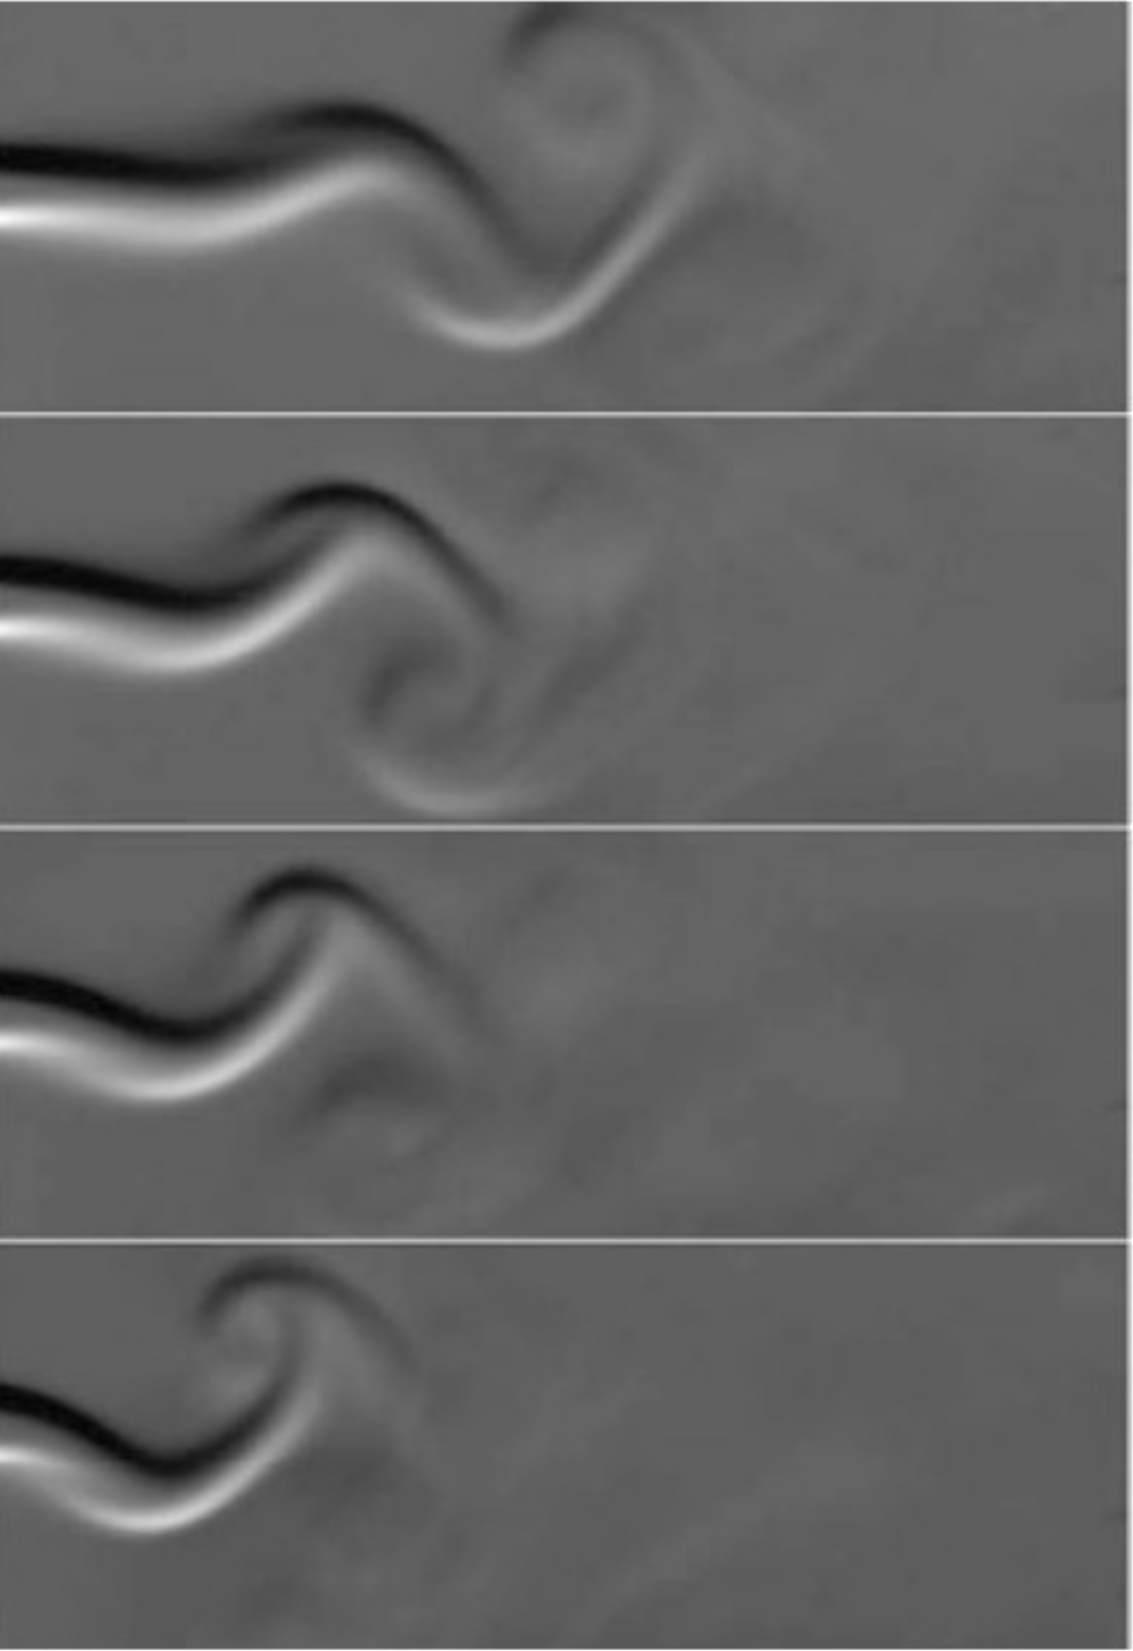
\includegraphics[height=0.3\textheight]{00_Images/07_chapter/14.png}
        \label{fig:jettransverse}
    } \hfill
    \subfloat[Turbulent Jet]{
        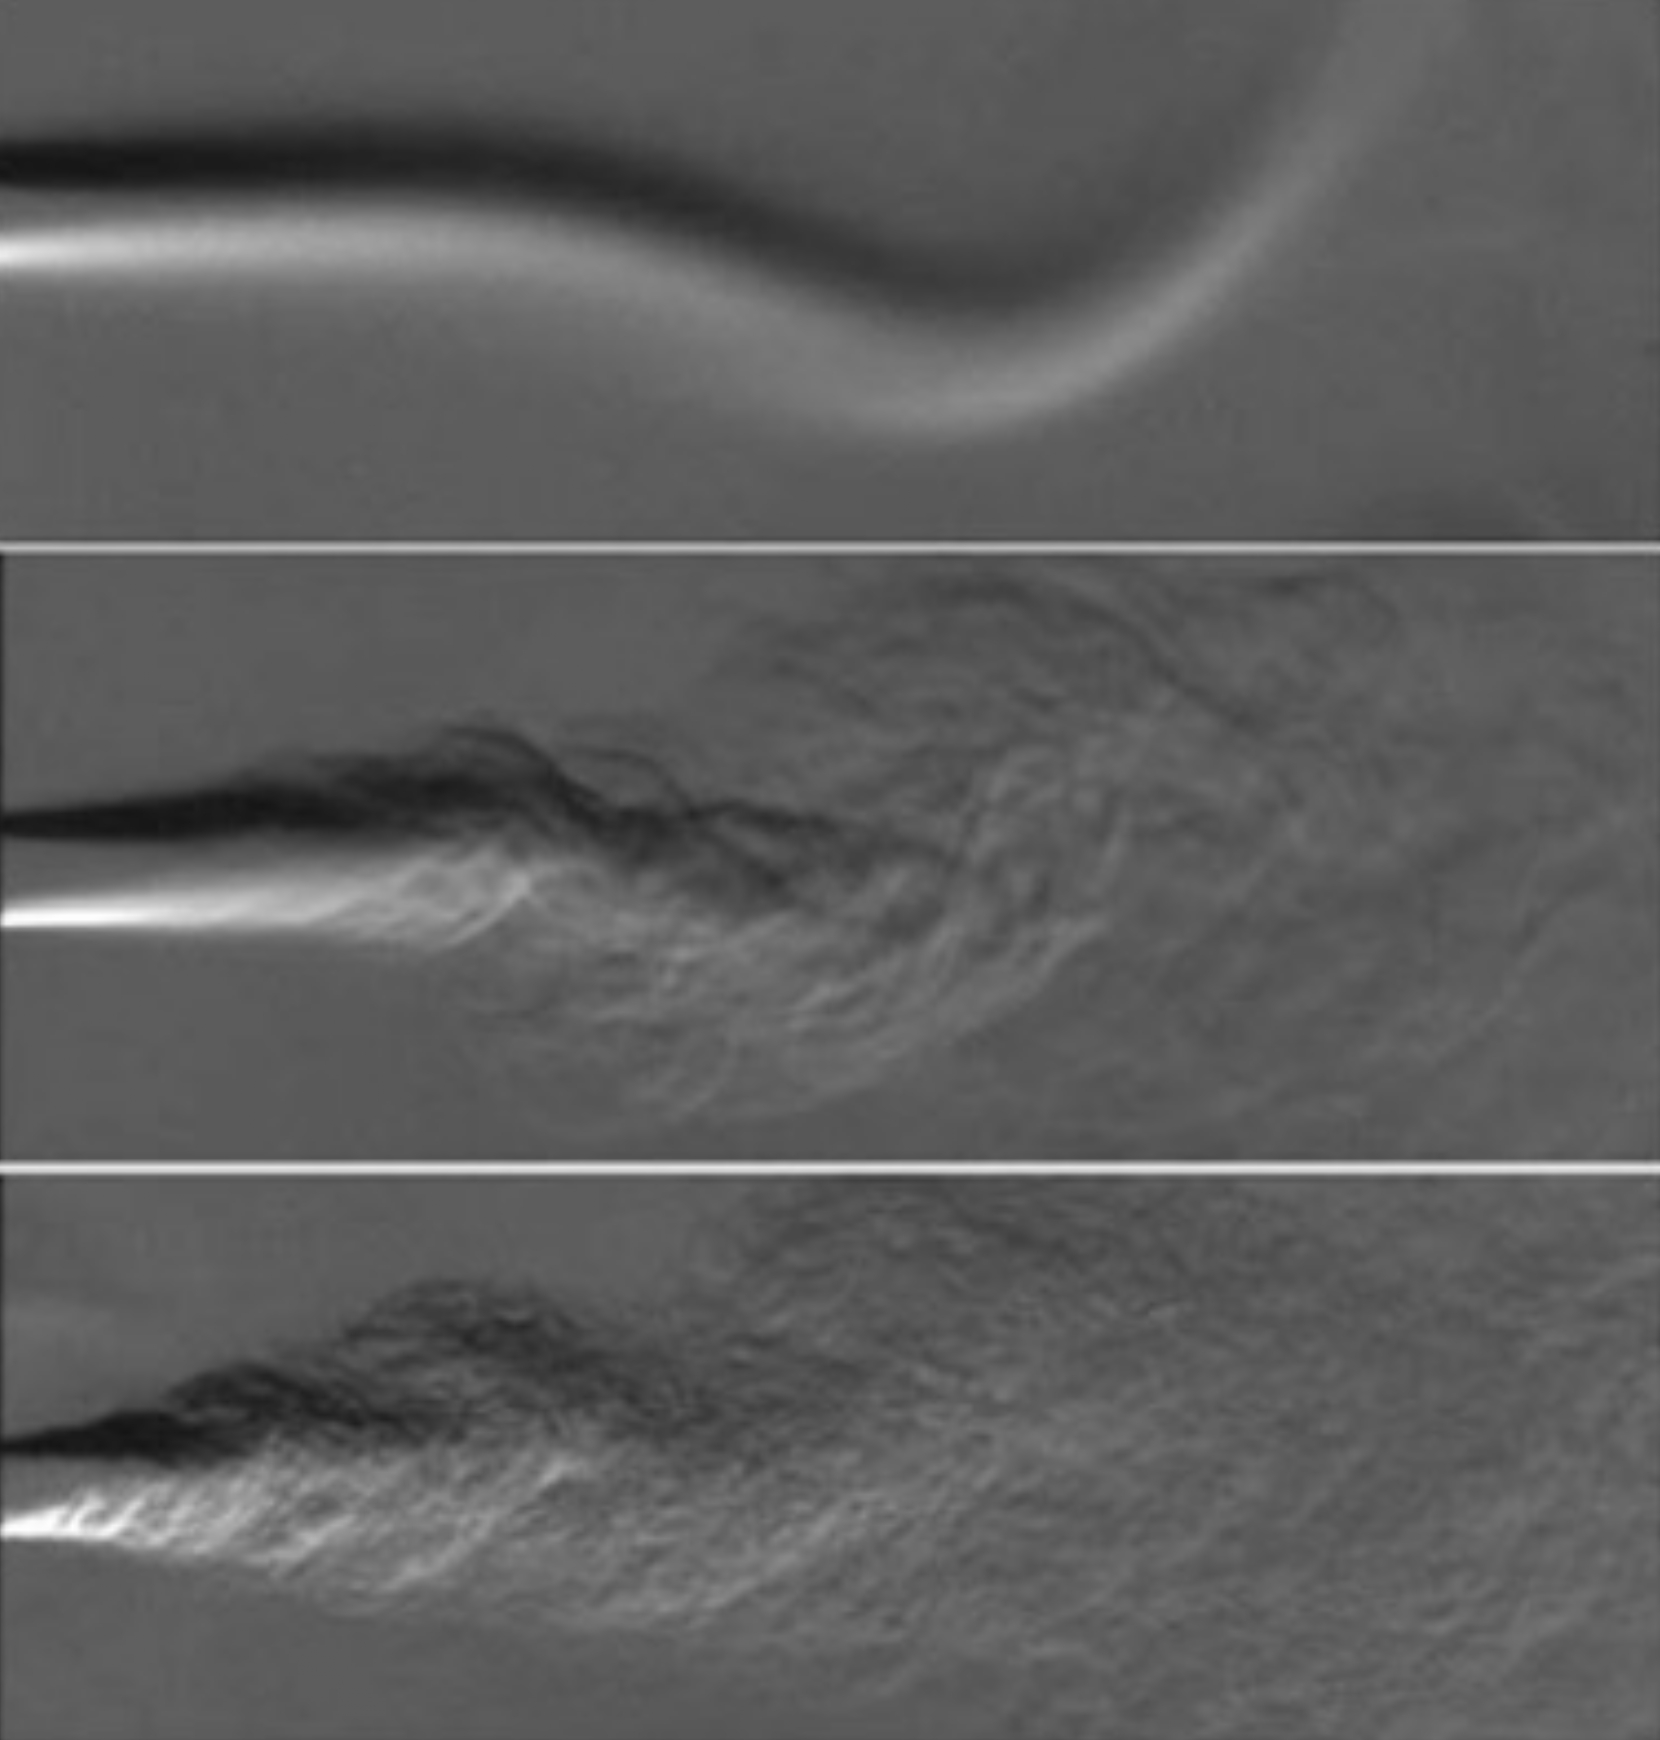
\includegraphics[height=0.3\textheight]{00_Images/07_chapter/15.png}
        \label{fig:turbolent}
    }
    \caption{Visualization of a jet subject to a transverse acoustic field and of a jet perturbed by an acoustic field}
\end{figure}

\section{The Aeroacoustic Source}

The interaction of the oscillating jet with the labium produces the acoustic energy that sustains the oscillation in the resonator. The largest jet oscillation takes place at a position where the resonator shows a strong reaction: the labium is an edge at an open pipe end, where the acoustic velocity is maximum. Furthermore, a sharp labium induces a local singularity in the acoustic field. The same jet oscillation in the free field or at a less reactive position in the resonator would not produce as much sound.

\section{The Jet-Drive Model}

\begin{figure}
    \centering
    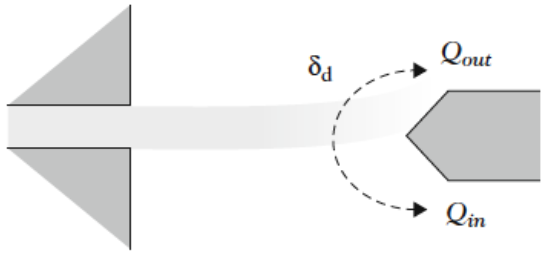
\includegraphics[width=0.7\linewidth]{00_Images/07_chapter/16.png}
    \caption{The jet-drive model}
    \label{fig:jetdrivemodel}
\end{figure}

\subsection{Dipole Source Representation}

This model is based on an idea by Helmholtz and Rayleigh. The model takes the two flow injections on both sides of the labium into account. The two sources (referencing to figure \ref{fig:jetdrivemodel}) \(Q_{\mathrm{in}}\) and \(Q_{\mathrm{out}}\) have fluctuating parts \(Q_1\) and \(Q_2\), placed a small distance \( \delta_d \) from each other, with opposite phases. They generate a pressure difference.

\subsection{Low-Frequency Approximation and Resonator as a Transmission Line}

The model is developed using a low-frequency approximation. Plane waves propagate in the resonator, which is therefore represented as a 1D transmission line. Assuming that the source dimensions are small compared to the acoustic wavelength, the resonator is described as the composition of a main pipe and a short, thinner pipe, since the open end in the mouthpiece always has a smaller cross-sectional area than the pipe.

\subsection{Force on the Acoustic Field}

The two sources with opposite phases \(Q_1\) and \(Q_2\) are placed in the thin short pipe at a short distance \( \delta_d \) from each other. They constitute a dipole confined in the small pipe of cross section \(S_m\) and produce an alternate motion of the air mass \( \rho\delta_d S_m \) between the two sources. The acceleration of this air mass generates the force acting on the acoustic field. This force can be expressed in terms of a pressure difference acting across the mouth of the pipe using the Euler equation.
\[
\frac{\partial p}{\partial x}=-\rho\frac{du}{dt} 
\quad \Rightarrow \quad
\frac{\Delta p}{\delta_d} \approx - \frac{\rho}{S_m} \frac{d Q_1}{dt}
\]

\subsection{Low Jet Velocity Relations}

For low jet velocities (Reynolds number below several hundred), it can be stated that
\[
\delta_d \approx \frac{\lambda_h}{2}
\qquad
\lambda_h=\frac{2\pi c_p}{\omega}
\qquad
c_p=\frac{\omega}{\alpha_r}
\]
In many cases,
\[
c_p=0.4U_j
\]
Defining \( \eta \) as the jet transverse displacement at the labium,
\[
Q_1 = H\int_{y_0}^{\infty}U(y-\eta)dy
\]
where \(H\) is the width of the jet at the labium. In many cases, \(H=h\) (flue channel thickness) and \(y_0\) is the transverse position of the labium. The displacement at the labium can be written as
\[
\eta(W,t)=\frac{h}{U_j}v_{\mathrm{ac}}\left(t-\frac{W}{c_p}\right)e^{\alpha_i W}
\]

\subsection{High Jet Velocity Scaling}

For high jet velocities, the acoustic power varies as the fourth power of the jet velocity, i.e., the Mach number,
\[
P_{\mathrm{ac}}\propto M^{4}
\qquad
M=\frac{U_0}{c}
\]
In sound synthesis by physical modeling, adding a broadband noise that follows this power law to the source terms improves the realism of the synthesis.

\subsection{Flow-Driven Excitation}

Since the deflection of the jet is the acoustic driving mechanism and since this is driven by the acoustic flow out of the mouth of the resonator, the system will work best when this flow is a maximum and therefore at an acoustic admittance maximum. This corresponds to a flow-driven excitation mechanism. This is in contrast with pressure-driven reed generators, which operate at an impedance maximum of the resonator.

\section{Nonlinearity and Harmonic Generation}

\subsection{Jet Velocity Profile}

Let us analyze what happens when there is an offset between the labium position and the flue channel exit. The velocity profile of the jet tends toward a smooth, bell-shaped form described by
\[
U(y) = U_0 \sech^{2}\left(\frac{y}{b}\right)
\]
where \(U_0\) and \(b\) vary along the jet.

\subsection{Flow into the Resonator with Labium Offset}

Consider the flow into the resonator when the jet tip is displaced by an amount \(h\) and the labium is displaced by \(h_0\) from the center of the jet. The corresponding flow is
\[
U_j
= W\int_{-\infty}^{h_0} U_0 \sech^{2}\left(\frac{y-h}{b}\right)dy
= W b U_0\left[\tanh\left(\frac{h_0-h}{b}\right) + 1\right]
\]
A jet with a top-hat velocity profile would yield a similar characteristic but with a sharper change in slope. This behavior is reported in figure \ref{fig:resonatorflow}.

\begin{figure}[!htb]
    \centering
    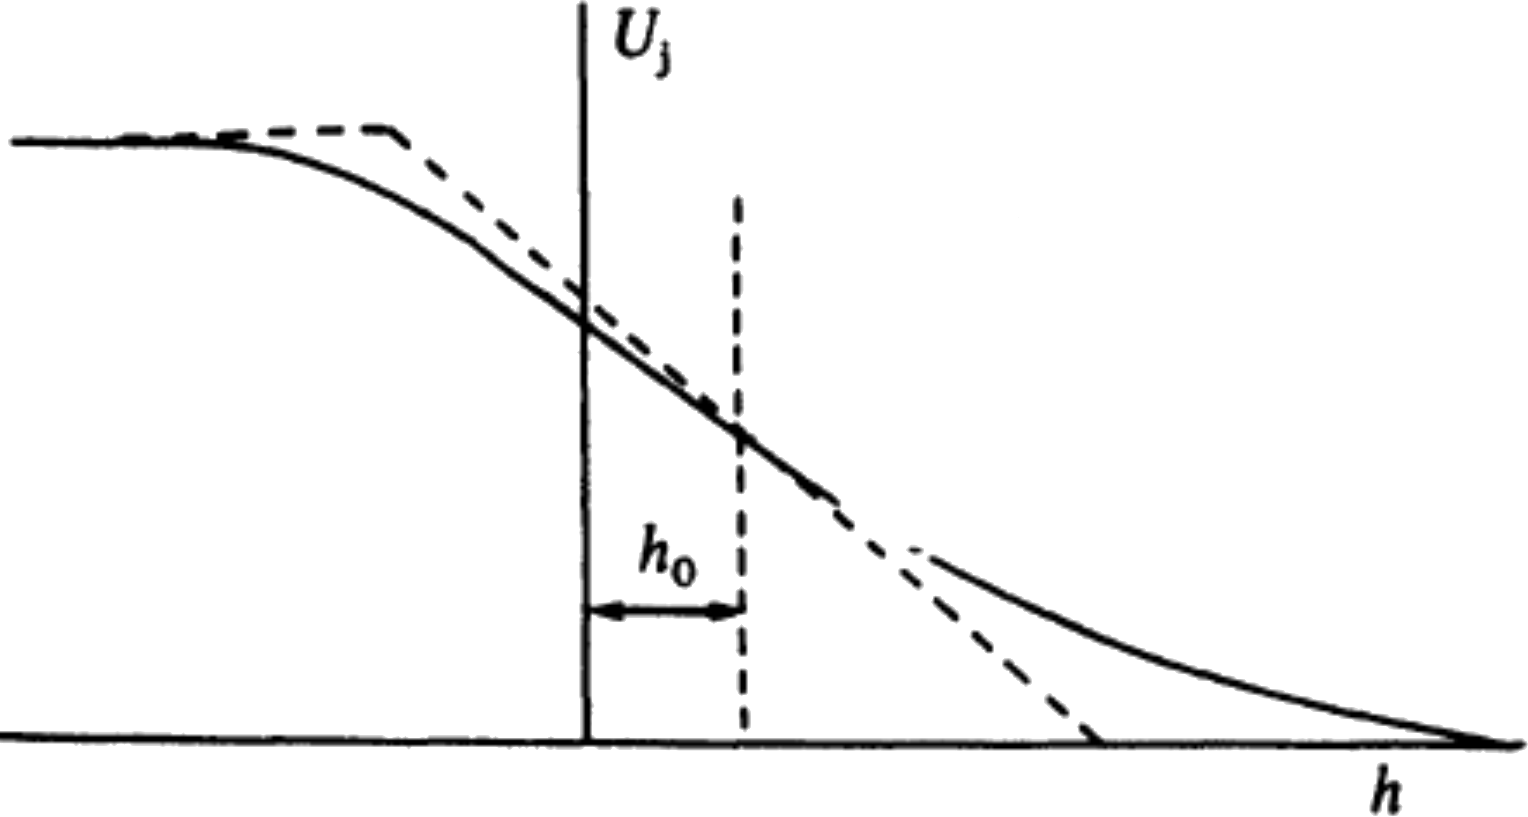
\includegraphics[width=0.7\linewidth]{00_Images/07_chapter/18.png}
    \caption{The flow into the resonator with labium offset}
    \label{fig:resonatorflow}
\end{figure}

\subsection{Sinusoidal Excitation and Harmonics}

Assume that the excitation is sinusoidal,
\[
h = a\cos\omega t
\]
If \(a<b\), the amplitude of the \(n\)-th harmonic varies approximately as \((a/b)^n\) and there is also a dependence on \(h_0/b\). If \(h_0=0\) the jet strikes the labium symmetrically and there are no even harmonics. If \(h_0 = 1.1b\), there is no third harmonic, but the first and second are strong. As an example, relative levels of the first four harmonics of the jet drive of an organ pipe as a function of the ratio of the offset \( h_0 \) of the jet relative to the jet half-width b are reported in figure \ref{fig:organflow}.

\begin{figure}[!htb]
    \centering
    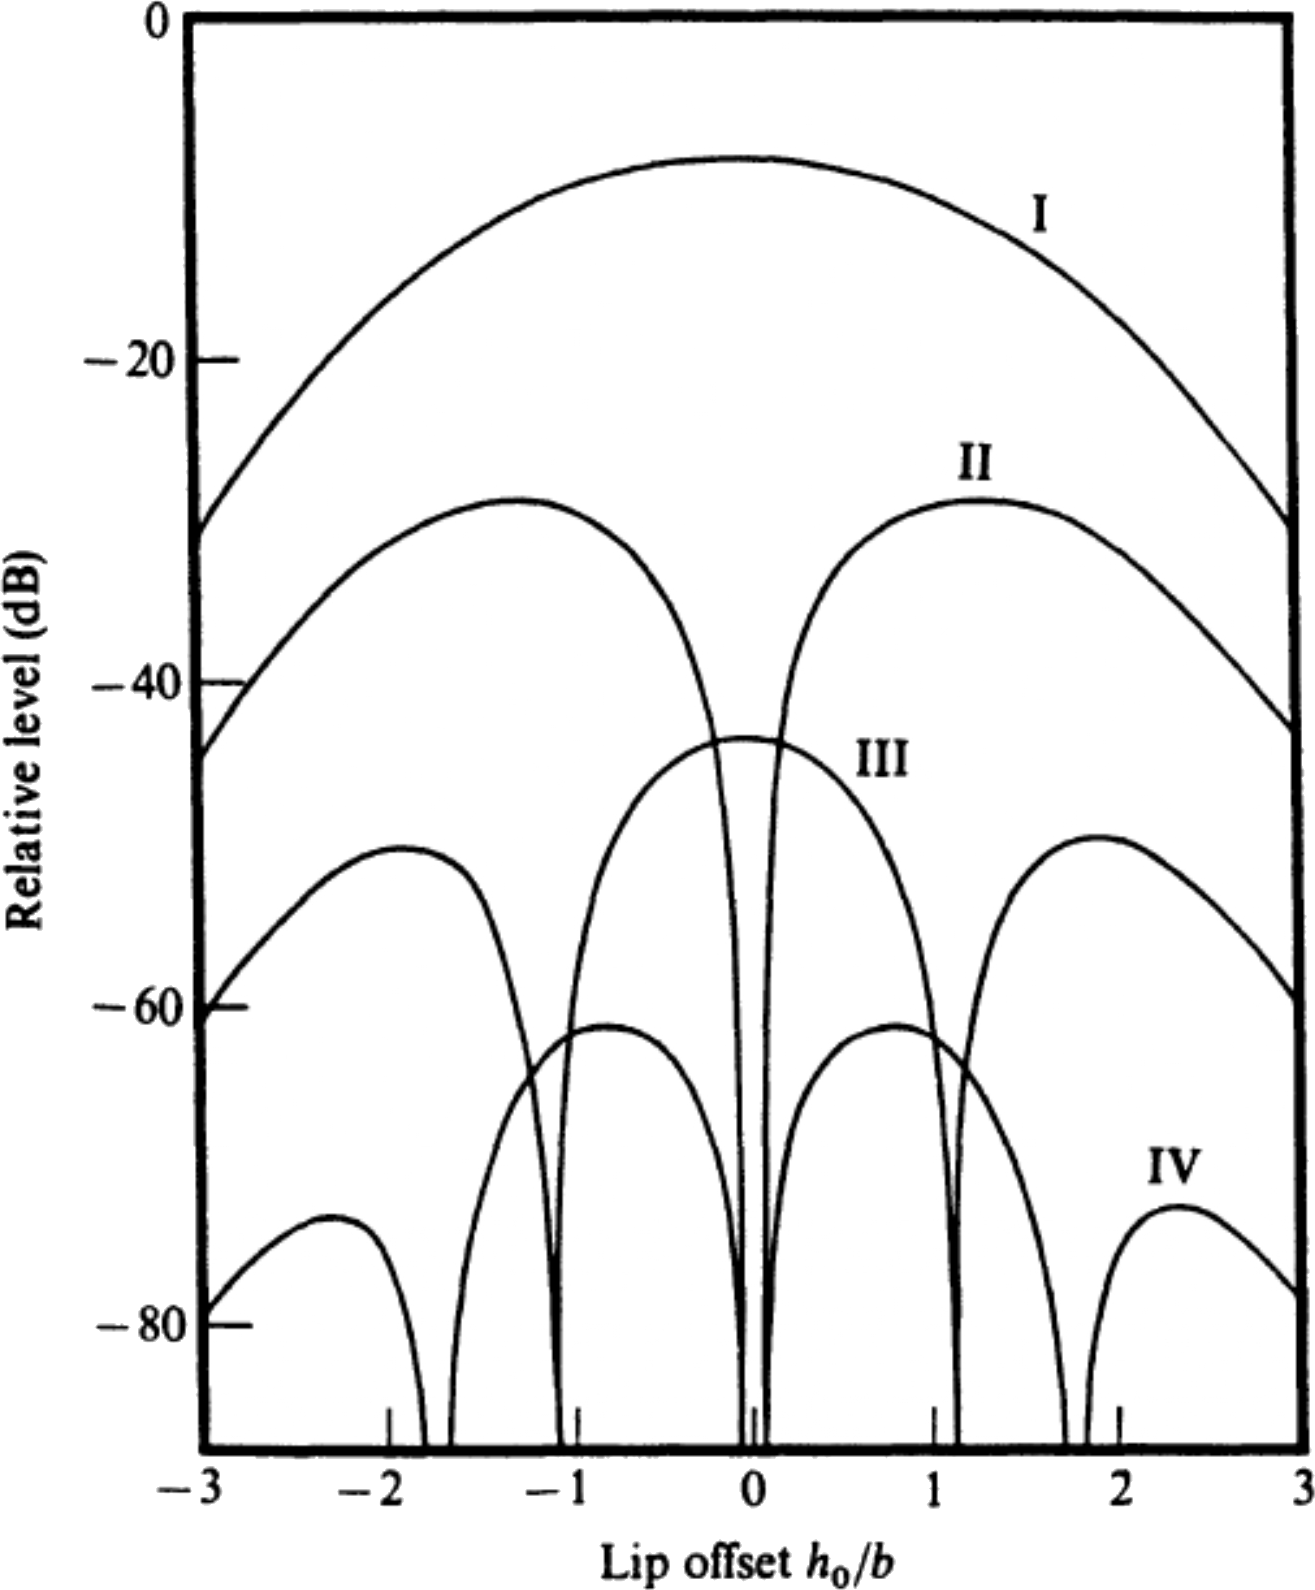
\includegraphics[height=0.3\textheight]{00_Images/07_chapter/19.png}
    \caption{Levels of the first four harmonics of the jet drive of an organ pipe}
    \label{fig:organflow}
\end{figure}

\subsection{Interaction With Pipe Resonances}

The presence of any upper harmonics in the pipe flow will be reflected in propagating waves of appropriate frequency on the jet and, consequently, in the further drive terms. The effect of this interaction is relatively small unless the jet length and velocity are such that it acts as a generator at the harmonic frequency. The relative level of upper harmonics in the sound is greatly influenced by the frequency alignment and \(Q\)-values of the upper pipe resonances.

\section{An Overview on Flute-Type Instruments}

\subsection{Panpipes and Shakuhachi}

The simplest type of flute-like instrument is the panpipes. There is a single pipe resonator for each note, made from bamboo cut so that its lower end is closed by a septum in the plant stem. The adjustment of the pipe length is then accomplished by pouring wax into the pipes. The instrument generally produces a simple diatonic major scale over a compass of about 1.5 to 2 octaves and is sounded by blowing across the top of each pipe, with the player's lower lip in contact with one edge of the pipe opening. The pipes are scaled so that their cross-sectional area is roughly proportional to length: long pipes are relatively narrower than short pipes. An incidental effect of the scaling of pipe diameter is a consequent scaling of jet length, which aids in the sounding of high notes. Since the jet length is decreased by a factor \(1/\sqrt{2}\) for an octave change in pitch, it is necessary to increase the jet speed by a factor \(\sqrt{2}\) or the blowing pressure by a factor \(2\) to maintain the appropriate phase relations. Since the pipe resonators are stopped at their lower ends, their resonance frequencies follow approximately an odd-harmonic series. Percussive breathy sounds can also be produced by deliberately failing to satisfy the normal regeneration conditions and blowing with a wide, turbulent jet; the acoustic spectrum then resembles the noise background. The shakuhachi is made from the root end of a bamboo plant and constitutes a nearly cylindrical, slightly curved, open tube. The mouth end has a bevel cut on one side that is fashioned to a sharp edge or may even have an ivory or agate wedge inserted. The player blows across the open end, but more into the instrument than for the panpipes. Since the tube is open, odd and even harmonics are comparably strong in the radiated sound. The shakuhachi has just five finger holes (two for the fingers of each hand and one for the left thumb) and is naturally adapted for traditional Japanese pentatonic music.

\subsection{The Recorder}

In the recorder family, the air jet is defined by an extended slit or windway; the shape of the mouth and labium is defined by the construction of the instrument and the notes of the scale are produced by opening finger holes. With the exception of the ocarina, the instruments of this family use a cylindrical or slightly tapering air column rather than a flaring one. Recorders have a very long history, but they are commonly divided into Renaissance recorders and Baroque recorders. Renaissance recorders have a nearly cylindrical bore and a simple outside form, while instruments of the Baroque style have a tapering conical bore, two or more separately jointed sections and decorative turning near the head and foot. Baroque recorders are made in a wide range of sizes.

\subsection{Recorder Bore and Resonance Conditions}

Neglecting the radiation load, an incomplete cone can be characterized through its input impedance \(Z_{\mathrm{in}}\), leading to the usual distinction between impedance zeros and impedance maxima. In particular, impedance maxima occur when \(\sin k(L+\theta_1)\) vanishes and relative to a cylindrical bore, the maxima are raised in frequency and do not lie midway between minima. The most relevant advantage of the conical bore with respect to the cylindrical one is constructional: careful tuning requires adjustments of the bore diameter at various places along its length, which can be built into a tapered reamer with consequent ease of adjustment and reproducibility. In a typical Baroque recorder, the main-bore taper corresponds to a conical semi-angle between \(0.5^\circ\) and \(1^\circ\) and the diameter at the foot end is typically \(0.5\) to \(0.7\) times that at the head. The resonance condition for the whole instrument is that the impedance of the air column in series with the impedance of the mouth window be a minimum. The mouth impedance \(Z_m\) is essentially an inertance \(j\omega M\). Equating the low-frequency form of a cylindrical-bore end correction to this inertance yields the constraint
\[
\Delta L = \frac{MS}{\rho}
\]
However, \(\Delta L\) decreases with frequency. This tends to stretch the intonation: high-note resonances are sharp and low-note resonances are flat. Players compensate by blowing low notes as strongly as possible to raise pitch and doing the opposite for high notes.

\subsection{The Flute}

With the term flute we refer typically to the transverse flute. Before Baroque times, flutes were generally cylindrical and this form was revised in the late seventeenth century. The Baroque flute, like the recorder, had a slightly tapered conical main bore and was divided into two or more sections, the head being nearly cylindrical. It had six main finger holes, an extra hole for the right-hand little finger and no thumb hole. Unlike the recorder, the flute continued to develop and progressively acquired keys between and below the six normal finger holes to allow accurate and even playing of chromatic semitones. The modern flute has a cylindrical bore about \SI{19}{\milli\meter} in diameter, except for the head joint, which contracts slightly to about \SI{17}{\milli\meter} toward the embouchure hole. It has 12 or 13 large holes and 3 small ones, all covered by padded keys and a unified mechanism that allows virtually any combination of holes to be closed without moving the fingers from their standard positions.

\subsection{Flute Head Joint: Cavity and Embouchure Hole}

\begin{figure}[!htb]
    \centering
    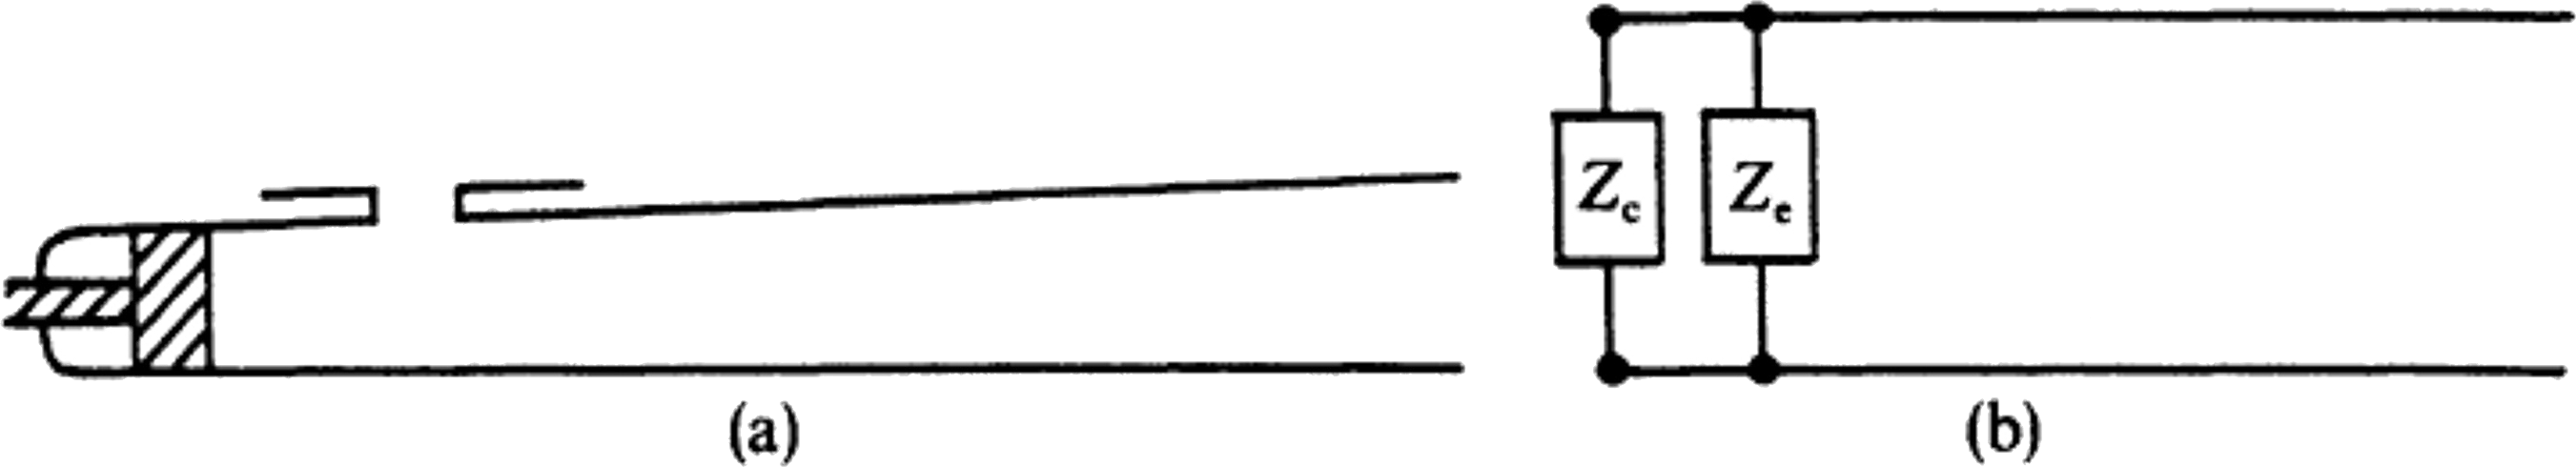
\includegraphics[width=0.7\linewidth]{00_Images/07_chapter/20.png}
    \caption{Tapered head joint of a modern flute and its equivalent network}
    \label{fig:flutescheme}
\end{figure}

Most important to the tuning and tonal quality of a flute are the bore profile of the head joint, the size of the cavity between the embouchure hole and the stopped end and the detailed shape of the embouchure hole. Of these, the most significant is the cavity above the embouchure hole: gross mispositioning of the stopper cork defining this cavity can mistune the two lower registers by as much as half a semitone relative to each other. Considering the scheme reported in figure \ref{fig:flutescheme}, the embouchure impedance \(Z_e\) is that of an inertance \(M\),
\[
Z_e = jM\omega = j\frac{\rho l_e \omega}{S_e}
\]
and the shading effect of the player’s lips must be taken into account in evaluating \(l_e\) and \(S_e\). The cavity impedance \(Z_c\) is that of an acoustic compliance \(C\),
\[
Z_c = \frac{1}{j\omega C} = -j\frac{\rho c^2}{\omega V}
\]
The characteristic impedance of the flute tube is
\[
Z_0 = \frac{\rho c}{S}
\]
and the impedance presented by embouchure hole and cavity in combination is equivalent to an end correction \(\Delta L\) defined by
\[
jZ_0\tan k\Delta L = (Z_e^{-1} + Z_c^{-1})^{-1}
\]
or
\[
\Delta L
= \frac{c}{\omega}\tan^{-1}\left[\frac{M\omega}{Z_0\bigl(1-MC\omega^2\bigr)}\right]
\]
In a normal head joint, \(\Delta L\) can be made nearly constant over the range \(0\)–\SI{2}{\kilo\hertz} if the stopper is set about \SI{17}{\milli\meter} from the center of the embouchure hole and \(\Delta L\) is then about \SI{42}{\milli\meter} with the player’s lips in normal position. Another important component is the embouchure hole itself. Early wooden flutes had a wall thickness at the head joint of about \SI{5}{\milli\meter} and almost any hole of reasonable size (e.g. \SIrange{7}{12}{\milli\meter} diameter) could function as an embouchure hole. For an average player, a hole about \SI{10}{\milli\meter} in diameter is best: a smaller one gives a soft, constricted sound, while a larger one is loud but less controlled. Boehm introduced a nearly rectangular hole, with dimensions close to \SI{10}{\milli\meter} by \SI{12}{\milli\meter}. In a metal flute the hole is built up using a chimney about \SI{5}{\milli\meter} in height, on top of which is the embouchure plate against which the player's lower lip rests.

    %! TEX rootmain.tex

\chapter{Drums}

Drums are percussion instruments in which vibrating membranes, often coupled to air volumes and supporting structures, generate sound after impulsive excitation. The perceived pitch, timbre, and decay depend on membrane modes, their coupling to enclosed air and shells, radiation efficiency, and playing technique. The discussion introduces common taxonomies for drums, then focuses on kettledrums, bass drums, snare drums, tom toms, drumhead construction variants, and selected Indian drums.

\section{Types of Percussions and Drums}

A practical distinction separates percussion instruments into pitched and unpitched families.

\begin{itemize}
    \item Pitched percussion instruments convey a strong sense of pitch; typical examples include kettledrums and tabla-type instruments.
    \item Non-pitched percussion instruments emphasize broadband or weakly tonal spectra; typical examples include snare drums, bass drums, tom toms, bongos, congas, and tambourines.
\end{itemize}

\section{Drum Categories}

A second categorization emphasizes how the membrane is coupled to an acoustic load and to structural elements.

\begin{itemize}
    \item Single membrane coupled to an enclosed air cavity, as in kettledrums.
    \item Single membrane mounted on resonant structures, as in congas or djemb\`e-type drums.
    \item Double membrane mounted on a shell, as in bass drums and snare drums.
\end{itemize}

This taxonomy highlights that the same vibrating element (a membrane) can lead to very different radiation and decay behaviors depending on the surrounding air volume and the mechanical boundary conditions set by the frame or shell.

\section{Kettledrums}

\subsection{Instrument Structure and Pitch Control}

Kettledrums (timpani) behave as pitched instruments. Pitch control is achieved through a pedal-operated mechanism that changes the membrane tension, hence shifting modal frequencies. The typical resonator is an approximately hemispherical bowl, often made of copper, and multiple timpani of different sizes are commonly used together in performance. 

\subsection{Harmonic Relationships and the Role of Air Loading}

An ideal membrane exhibits intrinsic inharmonicity, yet kettledrums can produce spectra with more nearly harmonic relationships. Several effects contribute to this partial regularization: 

\begin{itemize}
    \item air loading,
    \item coupling with shell resonances,
    \item air cavity resonances,
    \item membrane bending stiffness,
    \item membrane stiffness to shear.
\end{itemize}

Among these, air loading is the dominant factor in determining the pitched character. Air loading lowers the frequencies of low-order modes and adjusts their ratios toward more harmonic relationships, while the other effects mainly provide finer adjustments and strongly influence decay behavior. Air loading can be described by considering the pressure acting on both sides of the membrane. In a kettledrum, the internal pressure field is shaped by the enclosed cavity and by a small vent-hole placed at the bottom of the bowl, while external radiation provides a second pressure contribution on the outer side of the membrane. A representative comparison of modal ratios illustrates the trend. Modes \((1, 1)\), \((2, 1)\), \((3, 1)\), \((4, 1)\) that would appear at approximately \( 1.00 : 1.34 : 1.66 : 1.98 \) for an ideal membrane are shifted toward ratios close to \( 1.00 : 1.50 : 1.97 : 2.44 \) for a membrane mounted on a kettledrum-like structure. When air loading is present without hinging to a shell, ratios still remain relatively harmonic, around \( 1.00 : 1.47 : 1.91 : 2.36 \), indicating that the shell is less critical for harmonicity than the air loading itself. 

\paragraph{Remark on computed and measured frequencies} For a representative tension value \( T = \SI{3990}{\newton\per\meter} \), calculated modal frequencies can be compared with measured values, and the agreement supports the use of air-loading-based models as a primary explanation of timpani pitch behavior.

\subsection{Excitation, Spectrum Over Time, and Perceived Tone}

The standard striking position is approximately one quarter of the membrane radius inward from the edge. The striking position strongly influences the spectral balance: hitting at the center tends to produce a duller sound with reduced harmonic content, while off-center strikes excite a different mix of modes. Different partials exhibit different decay rates. Axisymmetric \((0, 1)\), \((0, 2)\), \((0, 3)\) modes damp out relatively quickly, whereas modes such as \((1, 1)\), \((2, 1)\), \((3, 1)\), \((4, 1)\) can persist longer and are excited by both central and standard strikes. The \((1, 1)\) mode is typically the longest-lasting and becomes central in determining the perceived tone. In this context, psychoacoustic reconstruction of a missing fundamental is not effective because the higher components required to imply the fundamental do not persist long enough. Therefore, the perceived tone is not governed by a true fundamental component but is strongly associated with the prominent and long-lasting \((1, 1)\) mode.

\subsection{Sound Radiation and Decay}

Modal decay times are closely linked to radiation efficiency. The kettledrum structure acts as a baffle for the membrane, and each membrane mode corresponds to a different multipole-like radiation pattern. The \((0, 1)\) mode behaves approximately like a monopole and radiates energy efficiently, leading to rapid energy loss and a short decay. The \((1, 1)\) mode behaves approximately like a dipole, radiating less efficiently and therefore persisting longer. As and example, in figure \ref{fig:timpanisoundspectra} different measured sound spectra are reported, respectively after \SI{0.03}{\second} for a and c and after \SI{1}{\second} for b and d.

\begin{figure}[!htb]
    \centering
    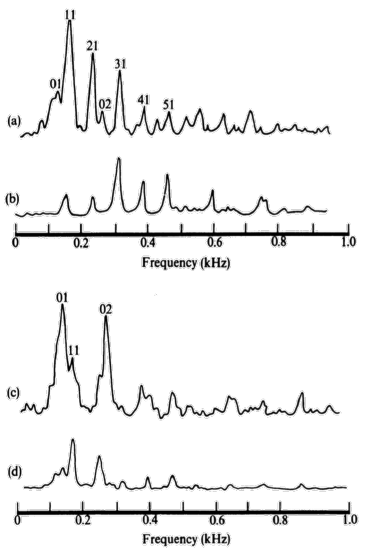
\includegraphics[height=0.3\textheight]{00_Images/08,09,10_chapter/01.png}
    \caption{Different sound spectra of a timpani}
    \label{fig:timpanisoundspectra}
\end{figure}

\section{Bass Drums}

\subsection{General Structure}

A bass drum typically mounts two membranes on opposite sides of a shell: a batter head and a resonant head. The tension relationship between these heads strongly influences timbre and partial decay times; commonly, the batter head is tuned to a higher tension than the resonant head. Bass drums are used as standalone orchestral instruments and as part of drum kits. 

\subsection{Modal Frequencies and Coupling of the Two Heads}

When the batter and resonant heads have the same tension, the coupled \((0, 1)\) behavior can be approximated by a two-mass oscillator. If \( f_0 \) denotes the frequency of either uncoupled head and \( f_a \) is a coupling frequency determined by the enclosed air stiffness and membrane masses, the normal modes occur at
\[
f_- = f_0
\]
and
\[
f_+ = \sqrt{ f_0^2 + 2 f_a^2 }
\]
In practice, the same mode index pair can appear at more than one frequency due to coupling effects, as illustrated by cases where a \((0, 1)\) pair is observed near both \SI{44}{\hertz} and \SI{104}{\hertz}. 

\subsection{Tension Relationship and Decay Rates}

When the batter head is overtensioned relative to the resonant head, modal decay rates are typically in the range \SIrange{3}{9}{\decibel\per\second}. In this configuration, removing the resonant head does not substantially change these decay rates. When both heads are tuned to the same tension, modes tend to decay faster, with rates around \SIrange{6}{11}{\decibel\per\second}. For lower-frequency modes with long wavelengths, decay also depends on interaction with the surrounding acoustic environment.

\subsection{Transient Tension Increase and Pitch Fall}

Immediately after a strong impact, the average membrane surface tension increases, producing an instantaneous rise in modal frequencies. As the tension relaxes back to its nominal value, modal frequencies decrease. This mechanism contributes to the characteristic pitch fall that can be heard in long-resonating bass drums struck with high force. 

\section{Snare Drums}

\subsection{General Structure and Materials}

A snare drum mounts two heads on the two sides of the shell. A set of snares (wires) is tightened against the resonant head, producing the characteristic buzzing component of the sound. Shells are commonly made of wood, such as maple, birch, or bubinga, or of metals, such as copper, brass, and steel. Marching-band snare drums differ markedly from typical drum-kit snares in construction and use.

\subsection{Lower-Mode Coupling as a Two-Mass Model}

The coupling of the first low-order modes of the two drumheads can be represented by a two-mass model in which the heads have different effective masses and spring constants. The coupled system is described by:

\begin{itemize}
    \item batter head mass \( m_b \) and spring constant \( K_b \),
    \item resonant head mass \( m_s \) and spring constant \( K_s \),
    \item coupling spring \( K_c \) associated with the enclosed air volume.
\end{itemize}

Introducing the angular-frequency parameters
\[
\omega_b^2 = \frac{K_b}{m_b} , \quad \omega_s^2 = \frac{K_s}{m_s} , \quad \omega_{cb}^2 = \frac{K_c}{m_b} , \quad \omega_{cs}^2 = \frac{K_c}{m_s}
\]
the two normal-mode angular frequencies satisfy
\[
\omega_{\pm}^2 = \frac{1}{2}\left( \omega_b^2 + \omega_s^2 + \omega_{cb}^2 + \omega_{cs}^2 \pm \sqrt{\left( \omega_b^2 + \omega_{cb}^2 - \omega_s^2 - \omega_{cs}^2 \right)^2 + 4 \omega_{cb}^2 \omega_{cs}^2} \right)
\]
These two normal modes combine on the two heads in a similar way and can be associated with the \((0, 1)\) behavior of the individual membranes. 

\subsection{Shell Modes and Possible Interactions}

The shell itself exhibits structural modal shapes even when drumheads are not mounted. These shell vibrations can contribute additional resonant features and participate in coupling mechanisms when heads are present, especially through the mechanical boundary conditions at the rims.

\begin{figure}[!htb]
    \centering
    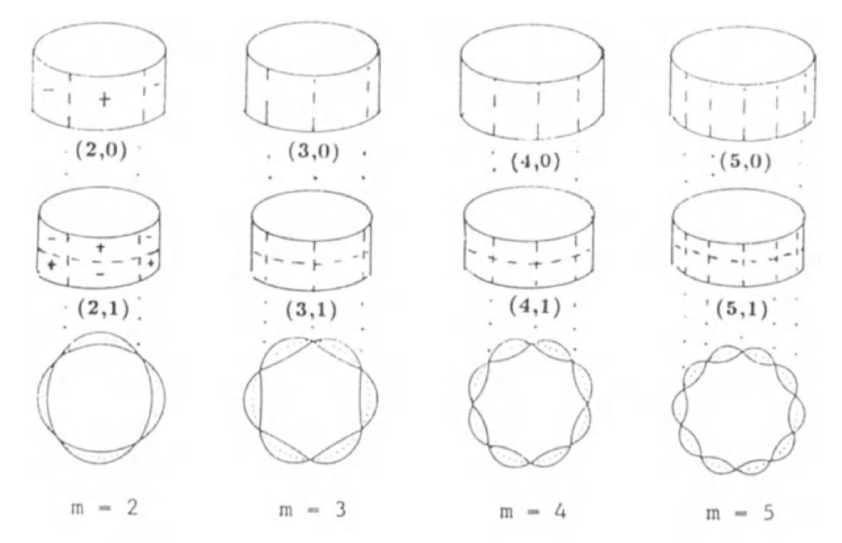
\includegraphics[width=0.7\linewidth]{00_Images/08,09,10_chapter/02.png}
    \caption{Snare shell modal shapes}
    \label{fig:snaremodal}
\end{figure}

\subsection{Snares Action}

Snares detach from the vibrating head and strike back against it, injecting high-frequency components into both the head motion and the snares themselves. Snare velocity depends on stroke intensity and snare tension, while low-tension snares produce greater damping of the resonant head. 

\section{Tom Toms}

Tom toms are used both as standalone instruments and as components of drum kits. Rack toms are typically mounted through suspension systems, while floor toms use legs to elevate the shell from the floor. The resonant head may be omitted in some designs, and open (single-head) toms tend to exhibit a clearer pitch character.

\section{Drumhead Types}

A wide variety of drumheads exists, and several construction features are commonly varied:

\begin{itemize}
    \item central reinforcement such as a power-dot,
    \item number of plies, including single-ply and double-ply heads,
    \item hydraulic film layers within double-ply heads,
    \item reinforcement rings,
    \item clear versus coated surfaces.
\end{itemize}

All these characteristics influence drum tone, harmonicity, and decay time by modifying the local mass, stiffness, and damping distributions on the membrane.

\section{Indian Drums}

\subsection{Tabla}

Tabla is typically played together with a larger bass companion instrument, often referred to as banya. A strong harmonic character is obtained by applying a central reinforcement to the drumhead. The head is commonly described as a multi-ply animal skin, and the central reinforcement can be produced by a paste made from boiled rice mixed with heavy metal particles. Tuning is achieved through the positioning of wooden cylinders within the leather thongs that tighten the head.

\paragraph{Remark on demonstrations} Short sound demonstrations are often used to emphasize the distinct tonal outcome produced by the reinforced central region.

\subsection{Mrudanga}

Mrudanga is a two-headed drum originating from southern India. The smaller head emulates the tabla-like behavior, while the larger head provides a bass response analogous to the banya. Similar drumhead treatments are applied on both sides to shape harmonicity. 

\subsection{Common Characteristics of Reinforced Indian Drumheads}

Reinforced Indian drumheads exhibit strong harmonic content, with the first four overtones often aligned as harmonics of the fundamental. Harmonic components can arise from combinations of several modes with very close frequencies. The harmonicity properties are attributed to the head reinforcement, which can be realized through many thin stacked layers, sometimes exceeding 100 layers; increasing the number of layers tends to increase harmonicity.

    %! TEX rootmain.tex

\chapter{Mallet Percussion Instruments}

Mallet percussion instruments belong to the family of idiophones, where the sound is produced by the vibration of the instrument body itself. In the tuned members of this family, pitch perception is shaped by the inharmonic modal structure of bars or rods and, when present, by auxiliary resonators that increase radiation efficiency and loudness. The chapter introduces a basic taxonomy of idiophones and then focuses on bar-based mallet instruments, discussing typical construction choices, overtone-tuning strategies, and the role of the mallet in controlling excitation bandwidth. The discussion is organized as follows:

\begin{itemize}
  \item idiophones and a basic classification into tuned and untuned instruments
  \item general features of mallet percussion instruments based on free bars or rods
  \item selected tuned bar instruments: glockenspiel, marimba, xylophone, and vibraphone
  \item the role of mallets in controlling spectral content through contact mechanics
\end{itemize}

\section{Idiophones}

Idiophones are instruments in which the sound is generated by the vibration of the whole object, without relying on dedicated vibrating elements such as strings or membranes. Depending on the instrument, vibration may be initiated by plucking, rubbing, or striking. Idiophones are commonly subdivided into one-dimensional and two-dimensional families, according to whether the dominant vibrating element behaves mainly like a bar/rod or like a plate. A further practical distinction is between tuned and untuned idiophones. Typical examples include:

\begin{itemize}
  \item tuned idiophones, such as xylophones, marimbas, vibraphones, bells, agogo and handpans,
  \item untuned idiophones, such as cymbals, tam-tams, triangles, and woodblocks.
\end{itemize}

\section{Mallet Percussion Instrument Characteristics}

A mallet percussion instrument is typically built as a collection of thin bars or rods with free ends. Each bar or rod behaves as a one-dimensional idiophone and is set into vibration by striking it with dedicated sticks called mallets. Because the flexural modes of free bars are not harmonically related, such instruments naturally exhibit an inharmonic overtone progression. For this reason, overtone tuning is often used to reshape selected modal frequencies so that the radiated spectrum supports a clearer pitch impression. When bars share the same geometry and size, the material plays a primary role in setting modal frequencies. The relevant elastic properties, and therefore stiffness, influence the characteristic velocity of mechanical-wave propagation in the bar, which in turn affects the modal frequencies set.

\section{Glockenspiel}

The glockenspiel uses rectangular steel bars, typically \SIrange{2.5}{3.2}{\centi\meter} wide and \SIrange{6}{9}{\milli\meter} thick. Its common range spans from G5 (\SI{784}{\hertz}) up to C8 (\SI{4186}{\hertz}). It is played with brass or plastic mallets. In this instrument, higher partials decay quickly and lie in a very high-frequency region, where pitch discrimination is reduced. As a consequence, little or no overtone tuning is typically pursued, and the sound rapidly settles to a recognizable pitch impression.

\subsection{Main Vibrational Modes}

Mode-shape diagrams (reported in figure \ref{fig:glockenspielmode}) commonly highlight a longitudinal mode and transverse modes in the plane of the bar (often indicated as the first and second transverse families). These families coexist and may contribute differently depending on the excitation point and mallet characteristics. 

\begin{figure}[!htb]
    \centering
    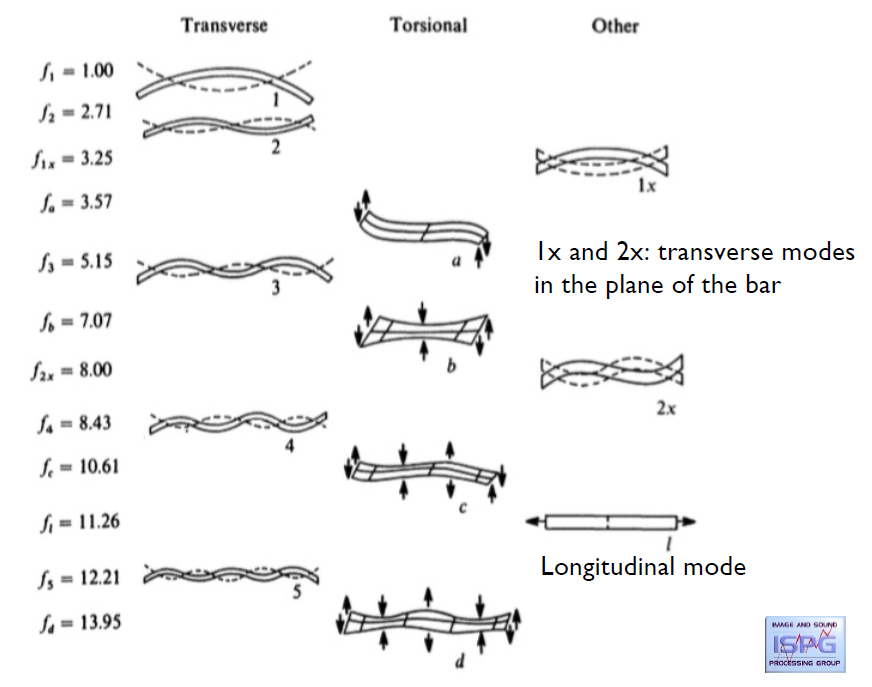
\includegraphics[width=0.7\linewidth]{00_Images/08,09,10_chapter/03.png}
    \caption{Glockenspiel main vibrational modes}
    \label{fig:glockenspielmode}
\end{figure}

\section{Marimba}

The marimba uses rectangular rosewood bars, typically \SIrange{4.5}{6.4}{\centi\meter} wide, arranged to cover about 3 to 4.5 octaves (often from A2 to C7, depending on the model). Under each bar, resonant tubes are positioned and tuned to the pitch of the corresponding bar. Unlike a simple rectangular section, marimba bars are shaped with an arched profile. This profile is a core design choice for both pitch range and spectral control.

\subsection{Marimba bars shape}

A section view of a marimba bar reveals the arched shape. This shaping serves two purposes: it allows lower pitches to be reached for a given bar length, and it enables overtone tuning. A common target is to tune the first overtone approximately two octaves above the fundamental, corresponding to a frequency ratio of about \( 4 \) relative to the fundamental. The associated mode-shape sketches typically show the transverse families for a tuned bar and the corresponding material-removal profile. A concise comparison between the modal shapes of standard rectangular bars and marimba bars is shown in figure \ref{fig:comparison}, highlighting how the location of displacement maxima shifts from the ends to the center and directly affects the optimal striking position for emphasizing specific overtones.

\begin{figure}[!htb]
    \centering
    \subfloat[Standard rectangula bar]{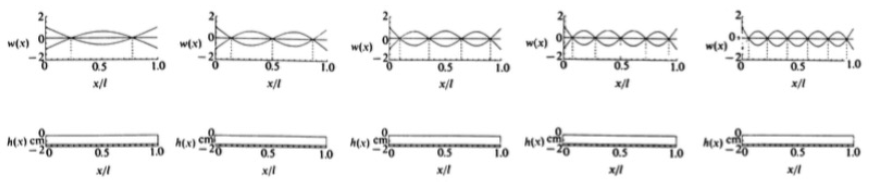
\includegraphics[width=0.7\linewidth]{00_Images/08,09,10_chapter/04_1.png}}\\
    \subfloat[Marimba bar]{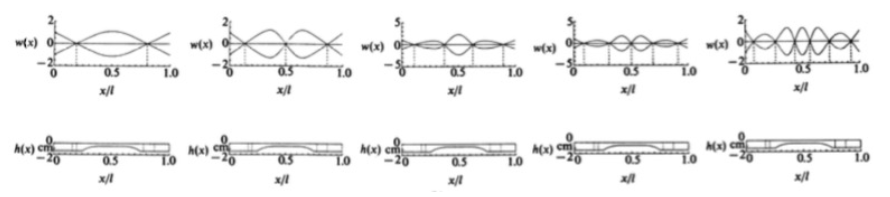
\includegraphics[width=0.7\linewidth]{00_Images/08,09,10_chapter/04_2.png}}\\
    \caption{Comparison between the modal shapes of standard rectangular bars and marimba bars}
    \label{fig:comparison}
\end{figure}

\paragraph{Where to Strike} A standard rectangular bar tends to have displacement maxima near the ends, whereas marimba bars are designed so that the displacement maximum occurs near the center. This matters for performance practice: the striking point can be chosen to emphasize or suppress specific overtones, depending on how strongly the impact couples into each modal shape.

\subsection{Tuning Procedures}

Material removal at selected points can be used to target individual modal frequencies. Removing material in regions where the bending moment of a given mode is large tends to lower the frequency of that mode significantly. Conversely, to raise the overall modal frequencies, material removal should be applied near the endpoints of the bar.

\subsection{Resonators}

Cylindrical pipe resonators, often closed at one end, are placed under each bar to emphasize the bar tone. The tube length is tuned to correspond to one quarter of the wavelength of the target bar tone, i.e., a quarter-wave relationship. The presence of resonators increases loudness while shortening decay time. In some listening conditions, this faster decay may still be perceived as a longer-lasting sound because the increased loudness remains above the ambient noise floor for longer. From a radiation viewpoint, the resonator increases acoustic efficiency by rephasing the field so that a dipole-like radiating bar behaves more like a monopole. This explains why the sound is louder and why energy is radiated away more efficiently, leading to faster decay. Closed-end resonators emphasize odd harmonics, so the resonator effect primarily influences the corresponding odd components of the bar spectrum. Even harmonics above the second are less affected. The distance between the bar and the resonator opening also matters because it affects the standing-wave pattern in the tube; in some designs, this distance can be adjusted to gently lower or raise tube resonances. A sketched representation of the sound decay with (line A) and without (line B) the resonators is reported in figure \ref{fig:decay}.

\begin{figure}[!htb]
    \centering
    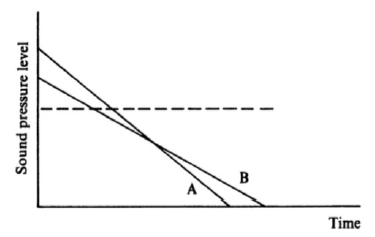
\includegraphics[width=0.5\linewidth]{00_Images/08,09,10_chapter/05.png}
    \caption{Sound decay with (line A) and without (line B) the resonators}
    \label{fig:decay}
\end{figure}

\section{Xylophone}

Modern xylophones are structurally similar to marimbas. A common difference is the absence of resonators, although some instruments may include them. The bars are often shaped underneath to manipulate overtone relationships. The overall sound character differs significantly: marimbas are typically duller and rounder, while xylophones are more brilliant and cutting. A typical tuning goal is to set the first overtone near three times the fundamental frequency, reinforcing a brighter, more incisive spectral profile.

\section{Vibraphone}

The vibraphone uses aluminum bars that are deeply arched, so the first harmonic occurs at approximately four times the fundamental frequency. Since aluminum decays more slowly than wood, a pedal-controlled damping mechanism is included, often implemented with a felt damper under the bars. A defining feature is the use of a mechanical motor to produce a vibrato-like effect, which motivates the instrument name.

\subsection{Motor-Driven Resonator Modulation}

Motor-driven disks on the resonators cyclically open and close the tubes. This periodic modulation produces an amplitude vibrato effect. Decay-rate plots typically show how the sustained tone is shaped over time in the presence of this modulation. A sketched representation of the sound decay is reported in figure \ref{fig:decayvibra}.

\begin{figure}[!htb]
    \centering
    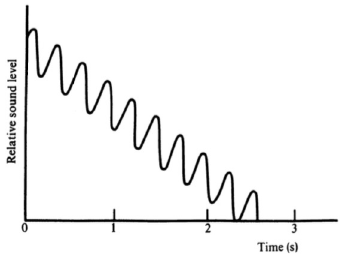
\includegraphics[width=0.5\linewidth]{00_Images/08,09,10_chapter/06.png}
    \caption{Sound decay of a vibraphone}
    \label{fig:decayvibra}
\end{figure}

\section{Mallets}

A wide variety of mallets exists, and mallet characteristics strongly influence the timbre by changing how energy is delivered to the bar and which frequency regions are excited. Three key parameters are typically emphasized:

\begin{itemize}
  \item hardness, since harder mallets more readily excite higher overtones, while softer mallets yield a rounder sound
  \item mass, which contributes to the energy transferred and, through inertia, affects contact time; longer contact times tend to damp higher partials more strongly
  \item impact velocity, which also affects contact time and mallet deformation; increased deformation can raise effective stiffness during contact and influence the highest harmonic efficiently excited
\end{itemize}

Figure \ref{fig:mallet} reports plots comparing different mallets report the maximum frequency effectively solicited as a function of impact velocity for mallets of different hardness, illustrating how the excitation bandwidth evolves with playing intensity.

\begin{figure}[!htb]
    \centering
    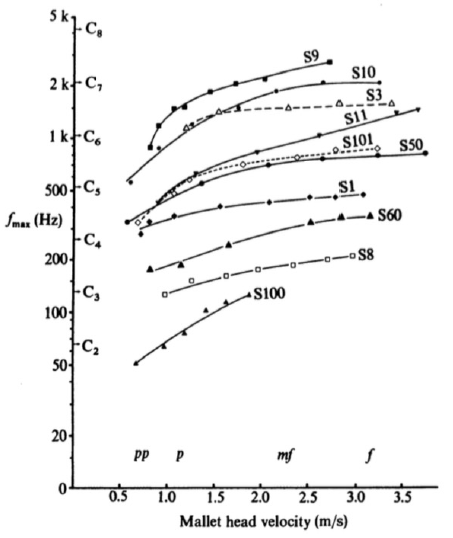
\includegraphics[height=0.3\textheight]{00_Images/08,09,10_chapter/07.png}
    \caption{Comparison between different mallets}
    \label{fig:mallet}
\end{figure}
    %! TEX rootmain.tex

\chapter{Cymbals, Tam-Tams, and Gongs}

This chapter focuses on two-dimensional metallic idiophones whose sound is dominated by a dense set of plate-like modes and strong nonlinear interactions. Cymbals, tam-tams, and gongs exhibit pronounced time-evolving spectra: an initially broadband transient response progressively organizes into recognizable modal patterns and, in some cases, an apparent pitch glide may occur. The chapter is organized as follows: 

\begin{itemize}
  \item modes of vibration of cymbals
  \item cymbals frequency spectrum
  \item transient and nonlinear behavior
  \item chaotic vibration
  \item tam-tams
  \item gongs
\end{itemize}

\section{Modes of Vibration of Cymbals}

Cymbals are almost always supported at their center, so the central region behaves as a node for essentially every vibration mode. For this reason, at low frequency the observable mode shapes are close to those of flat circular plates: modal frequencies are relatively well separated and individual patterns can be distinguished. Modes are conveniently indexed by \((m, n)\), where \(m\) is the number of nodal diameters and \(n\) the number of nodal circles, leading to Chladni-like figures with star-shaped nodal lines radiating from the center and, when \(n > 0\), one or more concentric nodal rings. At higher frequencies, the modal density increases, and modes may form nearly degenerate pairs and combine (for example, pairs such as \((13, 0)\) and \((2, 2)\) in a 15'' cymbal), so both visual identification and spectral attribution become progressively more difficult. A comparison between theoretical and measured modes of a cymbal is reported in figure \ref{fig:cymbalmode}.

\begin{figure}[!htb]
    \centering
    \subfloat[Theoretical mode shapes]{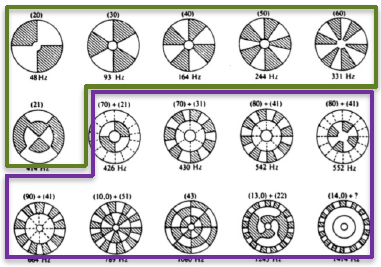
\includegraphics[height=0.2\textheight]{00_Images/08,09,10_chapter/08.png}} \hfill
    \subfloat[Measured mode shapes]{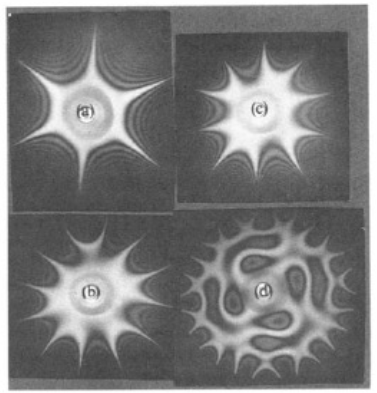
\includegraphics[height=0.2\textheight]{00_Images/08,09,10_chapter/09.png}}
    \caption{Comparison between theoretical and measured mode shapes}
    \label{fig:cymbalmode}
\end{figure}

\section{Cymbals Frequency Spectrum}

Modal frequencies are often approximated by a Chladni-like law in which the frequency depends on the nodal indices:
\[
f_{m,n} = c (m + 2n)^{p}
\]
Experiments indicate that a single slope does not fit the full modal set. Beyond a knee value \(m_c\), defined as a threshold in the number of nodal diameters, a different exponent and prefactor are required to follow the measured trend. This behavior is consistent with the fact that higher-order modes become more crowded and tend to exhibit stronger near-degeneracy and mixing, so the empirical scaling of \(f_{m,n}\) with \(m\) changes. A convenient representation is the piecewise model: 
\[
f_{m,n} =
\begin{cases}
c_1 (m + 2n)^{p_1}, & m \le m_c \\
c_2 (m + 2n)^{p_2}, & m > m_c
\end{cases}
\]

\section{Nonlinear and Transient Behavior}

\subsection{Spectral Evolution and Mode Coupling}

After a strike, cymbal sound evolves markedly over time. Nonlinear coupling among modes produces a large number of high-frequency partials, which are characteristic of cymbal timbre. Due to dispersion, high-frequency components can establish early, even before low-frequency standing-wave patterns become clearly recognizable. After an initial period that can be described as chaotic wave propagation, stable standing-wave patterns develop and correspond to the cymbal normal modes. Nonlinear phenomena may also favor the establishment of particular modal components, yielding an apparent pitch glide upward or downward, depending on the specific cymbal.

\subsection{Origin of the Nonlinearity}

A primary reason for strong nonlinear behavior is that the metal is thin, so tension and restoring forces are comparatively small. In this condition, the quadratic tension generated by modal displacements can have a large effect. Surface irregularities and hammering marks further facilitate coupling because abrupt spatial changes in displacement are known to ease energy exchange among modes.

\subsection{A Minimal Modal Picture}

A compact description treats each mode \(j\) as approximately sinusoidal with a slowly varying amplitude:
\[
y_j(t) = a_j(t) \sin(\omega_j t + \phi_j)
\]
For modes that are directly excited at the onset, a simple decay model is commonly assumed:
\[
a_i(t) = a_i \exp\left( - \frac{t}{\tau_i} \right)
\]
Upper modes may start with negligible energy and can grow through nonlinear coupling. In particular, energy transfer is emphasized when a near-integer relationship holds:
\[
\omega_j \approx n \omega_i
\]
In this picture, a coupled mode \(j\) may exhibit a delayed growth: its amplitude rises, reaches a maximum after a time \(t^\ast\), and then decays, consistent with the observed buildup and decay in different frequency bands:
\[
t^\ast = \frac{\tau_i \tau_j \ln\left( \tau_i / (n \tau_j) \right)}{\tau_i - n \tau_j}
\]
with the condition \( \tau_i > n \tau_j \). 

\section{Chaotic Vibration}

Cymbals behave as highly nonlinear systems: the fully developed sound after an arbitrary excitation depends strongly on chaotic behavior and cannot be easily described in detail. Even under sinusoidal excitation, a linear response is observed only for low amplitude forcing, whereas large amplitude forcing can suddenly establish additional frequencies associated with nonlinear interactions. Low-order modes can excite higher modes, which may combine and, in turn, drive further modes, yielding a cascade that sustains a chaotic regime before more stationary modal patterns become apparent.

\section{Tam-Tams}

Tam-tams can be regarded as oriental cymbals capable of producing very loud sounds. Their sound evolves strongly over time: it may begin with a very low-pitch impression and then nonlinearly build up higher and louder harmonics, raising the perceived pitch. Sustain can last for dozens of seconds. Higher harmonics vanish faster, and the late-time sound becomes dull again, similarly to the initial instants of vibration. A densely hammered surface enhances nonlinearities and contributes to this pronounced time evolution.

\section{Gongs}

Gongs share similarities with tam-tams but typically include a central dome. The dome strengthens tonal characteristics relative to tam-tams, and the first two axisymmetric modes often exhibit strong harmonic relationships. As for tam-tams, the spectrum becomes richer some time after the strike, consistent with the nonlinear buildup of additional components. The evolution can be described as a transition from a small number of prominent components at onset to a denser set of partials at intermediate times. 

    
\end{document}
